% UCL Thesis LaTeX Template
%  (c) Ian Kirker, 2014
% 
% This is a template/skeleton for PhD/MPhil/MRes theses.
%
% It uses a rather split-up file structure because this tends to
%  work well for large, complex documents.
% We suggest using one file per chapter, but you may wish to use more
%  or fewer separate files than that.
% We've also separated out various bits of configuration into their
%  own files, to keep everything neat.
% Note that the \input command just streams in whatever file you give
%  it, while the \include command adds a page break, and does some
%  extra organisation to make compilation faster. Note that you can't
%  use \include inside an \include-d file.
% We suggest using \input for settings and configuration files that
%  you always want to use, and \include for each section of content.
% If you do that, it also means you can use the \includeonly statement
%  to only compile up the section you're currently interested in.
% You might also want to put figures into their own files to be \input.

% For more information on \input and \include, see:
%  http://tex.stackexchange.com/questions/246/when-should-i-use-input-vs-include


% Formatting and binding rules for theses are here: 
%  https://www.ucl.ac.uk/students/exams-and-assessments/research-assessments/format-bind-and-submit-your-thesis-general-guidance

% This package goes first and foremost, because it checks all 
%  your syntax for mistakes and some old-fashioned LaTeX commands.
% Note that normally you should load your documentclass before 
%  packages, because some packages change behaviour based on
%  your document settings.
% Also, for those confused by the RequirePackage here vs usepackage
%  elsewhere, usepackage cannot be used before the documentclass
%  command, while RequirePackage can. That's the only functional
%  difference as far as I'm aware.
\RequirePackage[l2tabu, orthodox]{nag}


% ------ Main document class specification ------
% The draft option here prevents images being inserted,
%  and adds chunky black bars to boxes that are exceeding 
%  the page width (to show that they are).
% The oneside option can optionally be replaced by twoside if
%  you intend to print double-sided. Note that this is
%  *specifically permitted* by the UCL thesis formatting
%  guidelines.
%
% Valid options in terms of type are:
%  phd
%  mres
%  mphil
%\documentclass[12pt,phd,draft,a4paper,oneside]{ucl_thesis}
\documentclass[12pt,phd,a4paper,oneside]{ucl_thesis}


% Package configuration:
%  LaTeX uses "packages" to add extra commands and features.
%  There are quite a few useful ones, so we've put them in a 
%   separate file.
% -------- Packages --------

% This package just gives you a quick way to dump in some sample text.
% You can remove it -- it's just here for the examples.
\usepackage{blindtext}

% This package means empty pages (pages with no text) won't get stuff
%  like chapter names at the top of the page. It's mostly cosmetic.
\usepackage{emptypage}

% The graphicx package adds the \includegraphics command,
%  which is your basic command for adding a picture.
\usepackage{graphicx}

% The float package improves LaTeX's handling of floats,
%  and also adds the option to *force* LaTeX to put the float
%  HERE, with the [H] option to the float environment.
\usepackage{float}

% The amsmath package enhances the various ways of including
%  maths, including adding the align environment for aligned
%  equations.
\usepackage{amsmath}

% Use these two packages together -- they define symbols
%  for e.g. units that you can use in both text and math mode.
\usepackage{gensymb}
\usepackage{textcomp}
% You may also want the units package for making little
%  fractions for unit specifications.
%\usepackage{units}


% The setspace package lets you use 1.5-sized or double line spacing.
\usepackage{setspace}
\setstretch{1.5}

% That just does body text -- if you want to expand *everything*,
%  including footnotes and tables, use this instead:
%\renewcommand{\baselinestretch}{1.5}


% PGFPlots is either a really clunky or really good way to add graphs
%  into your document, depending on your point of view.
% There's waaaaay too much information on using this to cover here,
%  so, you might want to start here:
%   http://pgfplots.sourceforge.net/
%  or here:
%   http://pgfplots.sourceforge.net/pgfplots.pdf
%\usepackage{pgfplots}
%\pgfplotsset{compat=1.3} % <- this fixed axis labels in the version I was using

% PGFPlotsTable can help you make tables a little more easily than
%  usual in LaTeX.
% If you're going to have to paste data in a lot, I'd suggest using it.
%  You might want to start with the manual, here:
%  http://pgfplots.sourceforge.net/pgfplotstable.pdf
%\usepackage{pgfplotstable}

% These settings are also recommended for using with pgfplotstable.
%\pgfplotstableset{
%	% these columns/<colname>/.style={<options>} things define a style
%	% which applies to <colname> only.
%	empty cells with={--}, % replace empty cells with '--'
%	every head row/.style={before row=\toprule,after row=\midrule},
%	every last row/.style={after row=\bottomrule}
%}


% The mhchem package provides chemistry formula typesetting commands
%  e.g. \ce{H2O}
%\usepackage[version=3]{mhchem}

% And the chemfig package gives a weird command for adding Lewis 
%  diagrams, for e.g. organic molecules
%\usepackage{chemfig}

% The linenumbers command from the lineno package adds line numbers
%  alongside your text that can be useful for discussing edits 
%  in drafts.
% Remove or comment out the command for proper versions.
%\usepackage[modulo]{lineno}
% \linenumbers 


% Alternatively, you can use the ifdraft package to let you add
%  commands that will only be used in draft versions
%\usepackage{ifdraft}

% For example, the following adds a watermark if the draft mode is on.
%\ifdraft{
%  \usepackage{draftwatermark}
%  \SetWatermarkText{\shortstack{\textsc{Draft Mode}\\ \strut \\ \strut \\ \strut}}
%  \SetWatermarkScale{0.5}
%  \SetWatermarkAngle{90}
%}


% The multirow package adds the option to make cells span 
%  rows in tables.
\usepackage{multirow}
\usepackage{array} % For the tables in introduction

% Subfig allows you to create figures within figures, to, for example,
%  make a single figure with 4 individually labeled and referenceable
%  sub-figures.
% It's quite fiddly to use, so check the documentation.
%\usepackage{subfig}

% The natbib package allows book-type citations commonly used in
%  longer works, and less commonly in science articles (IME).
% e.g. (Saucer et al., 1993) rather than [1]
% More details are here: http://merkel.zoneo.net/Latex/natbib.php
%\usepackage{natbib}

% The bibentry package (along with the \nobibliography* command)
%  allows putting full reference lines inline.
%  See: 
%   http://tex.stackexchange.com/questions/2905/how-can-i-list-references-from-bibtex-file-in-line-with-commentary
\usepackage{bibentry} 

% The isorot package allows you to put things sideways 
%  (or indeed, at any angle) on a page.
% This can be useful for wide graphs or other figures.
%\usepackage{isorot}

% The caption package adds more options for caption formatting.
% This set-up makes hanging labels, makes the caption text smaller
%  than the body text, and makes the label bold.
% Highly recommended.
\usepackage[format=hang,font=small,labelfont=bf]{caption}

% If you're getting into defining your own commands, you might want
%  to check out the etoolbox package -- it defines a few commands
%  that can make it easier to make commands robust.
\usepackage{etoolbox}

% The microtype package adds `micro-typographic extensions' which
% generally makes text more readable and hyphenation less likely.
\usepackage{microtype}

% Packages for math typesetting
\usepackage{amsfonts}
\usepackage{amssymb}
\usepackage{amsthm}
\usepackage{mathpartir}
%\usepackage{palatino,mathpazo} % add possibly `sc` and `osf` options
\usepackage[T1]{fontenc}
\usepackage[utf8]{inputenc}
\usepackage[mathscr]{eucal}
%\usepackage{titlesec}
\usepackage{bm}
%\usepackage[svgnames]{xcolor}
\usepackage[all,cmtip,2cell]{xy}
\usepackage{enumerate}
\usepackage{graphicx}
\usepackage{stmaryrd}
\usepackage{rotating}
\usepackage{enumitem}
\usepackage{algorithm}
\usepackage{algorithmic}
\usepackage{interval}
%for convex algebra singature in chapter four
\usepackage{scalerel}
%for the xRightarrow
\usepackage{mathtools}
%for diagrams
\usepackage{quiver}
%For figure with axioms in chapter 4
\usepackage{multicol}
%For automata figures in chapter 4
\usepackage{cancel}
%For referencing one of the lemmas in the appendix
\usepackage{thm-restate}
%tikz setup for chapter three
\usepackage{tikz}
\usetikzlibrary{arrows,snakes,automata,backgrounds,petri, positioning,calc,cd, automata}
\usetikzlibrary{shapes.geometric,shapes.misc,matrix,arrows.meta,decorations.markings}
\tikzset{x=1em, y=1.5ex, baseline=-0.5ex}
\tikzset{ihbase/.style={inner sep=0,circle,draw,fill=lightgray,minimum size=0.4em,node contents={}}}
\tikzset{ihblack/.style={ihbase,fill=black}}
\tikzset{ihwhite/.style={ihbase,fill=white}}
\tikzset{mat/.style={draw,fill=white,rectangle,node font=\scriptsize}}
\tikzset{ha/.style={mat,rounded rectangle,rounded rectangle left arc=none}}
\tikzset{haop/.style={mat,rounded rectangle,rounded rectangle right arc=none}}
\tikzset{blackha/.style={mat,rounded rectangle,rounded rectangle left arc=none,font=\color{white},fill=black}}
\tikzset{blackhaop/.style={mat,rounded rectangle,rounded rectangle right arc=none,font=\color{white},fill=black}}
\tikzset{anti/.style={inner sep=0,isosceles triangle,fill=black,draw=black, minimum width=0.75em, node contents={}}}
\tikzset{antiop/.style={anti,shape border rotate=180}}
\tikzset{antisq/.style={inner sep=0,rectangle,fill=black, minimum height=1em, minimum width=0.6em, node contents={}}}
\tikzset{count/.style={above,inner ysep=0.15em,font=\scriptsize}}
\tikzset{axiom/.style={above,font=\small}}
\tikzset{dir/.style={-Latex}}
\tikzset{st/.style={decoration={markings,
    mark={at position 0.5 with {\draw (0, 2pt) to (0, -2pt);}}},
    postaction=decorate}}
% end of tikz setup


% Sets up links within your document, for e.g. contents page entries
%  and references, and also PDF metadata.
% You should edit this!
%%
%% This file uses the hyperref package to make your thesis have metadata embedded in the PDF, 
%%  and also adds links to be able to click on references and contents page entries to go to 
%%  the pages.
%%

% Some hacks are necessary to make bibentry and hyperref play nicely.
% See: http://tex.stackexchange.com/questions/65348/clash-between-bibentry-and-hyperref-with-bibstyle-elsart-harv
\usepackage{bibentry}
\makeatletter\let\saved@bibitem\@bibitem\makeatother
\usepackage[pdftex,hidelinks]{hyperref}
\usepackage{cleveref}
\makeatletter\let\@bibitem\saved@bibitem\makeatother
\makeatletter
\AtBeginDocument{
    \hypersetup{
        pdfsubject={Thesis Subject},
        pdfkeywords={Thesis Keywords},
        pdfauthor={Author},
        pdftitle={Title},
    }
}
\makeatother
    


% And then some settings in separate files.
\input{FloatSettings} % For things like figures and tables
\usepackage[
  backend=biber, 
  style=alphabetic,
  url = false,
  doi = false,
  maxbibnames = 10,
  backref = true
]{biblatex}   % For bibliographies
\addbibresource{example.bib}
% These control how many number sections your subsections will take
%    e.g. Section 2.3.1.5.6.3
%  and how many of those will get put into the contents pages.
\setcounter{secnumdepth}{3}
\setcounter{tocdepth}{3}

\newcommand{\printpublication}[1]{\AtNextCite{\defcounter{maxnames}{99}}\fullcite{#1}}

% Things shared between chapters
\newcommand{\alphabet}{\Sigma}
\newcommand{\seq}{\mathbin{;}} %Sequential composition of (probabilistic) regular expressions
\newcommand{\zero}{\mathsf{0}} %0 of a (probabilistic) regular expression
\newcommand{\one}{\mathsf{1}} %1 of a (probabilistic) regular expression
\newcommand{\sem}[1]{\left\llbracket{#1}\right\rrbracket}

% common behavioural distances stuff
\newcommand{\disteq}[1]{\equiv_{#1}} % rational-indexed equality
\newcommand{\e}{\varepsilon} % epsilon for distances
\newcommand{\PMet}{\mathsf{PMet}}

% chapter two only
\newcommand{\RExp}{\mathsf{RExp}}

\newcommand{\objr}{\blacktriangleright}
\newcommand{\objl}{\blacktriangleleft}
\newcommand{\arrowright}{\tikzfig{lr-order}}
\newcommand{\arrowleft}{\tikzfig{rl-order}}

%%%%%%%%%%%%%%%%%%%%%%%%%%%%%%%%%%%%%%%%%%%%%%%%%%%%%%%%%%%%%%%%%%%%%%%%%%%%%
%                          ROBIN'S TIKZ STUFF
%%%%%%%%%%%%%%%%%%%%%%%%%%%%%%%%%%%%%%%%%%%%%%%%%%%%%%%%%%%%%%%%%%%%%%%%%%%%%

\pgfdeclarelayer{edgelayer}
\pgfdeclarelayer{nodelayer}
\pgfsetlayers{edgelayer,nodelayer,main}

\definecolor{light-gray}{gray}{.5}
\tikzstyle{right arrow} = [->]
\tikzstyle{none}=[inner sep=0pt]
\tikzstyle{plain}=[inner sep=0pt]
\tikzstyle{black}=[circle, draw=black, fill=black, inner sep=0pt, minimum size=4pt]
\tikzstyle{black-faded}=[circle, draw=light-gray, fill=light-gray, inner sep=0pt, minimum size=4pt]
\tikzstyle{white}=[circle, draw=black, fill=white, inner sep=0pt, minimum size=4.5pt]
\tikzstyle{white-faded}=[circle, draw=light-gray, fill=white, inner sep=0pt, minimum size=4.5pt]
\tikzstyle{delay}=[fill=black, regular polygon, regular polygon sides=3,rotate=-90, scale=.55]
\tikzstyle{delay-op}=[fill=black, regular polygon, regular polygon sides=3,rotate=90, scale=.55]
\tikzstyle{reg}=[draw, fill=white, rounded rectangle, rounded rectangle left arc=none, minimum height=1.2em, minimum width=1.4em, node font={\scriptsize}]
\tikzstyle{coreg}=[draw, fill=white, rounded rectangle, rounded rectangle right arc=none, minimum height=1.2em, minimum width=1.4em, node font={\scriptsize}]
\tikzstyle{basicb}=[draw, fill=white, rectangle, rounded corners, minimum height=1.6em, minimum width=1.4em]
\tikzstyle{basic box}=[draw, fill=white, rectangle, rounded corners, minimum height=1.6em, minimum width=1.4em]
\tikzstyle{smallb}=[draw, fill=white, rectangle, rounded corners, minimum height=1.2em, minimum width=1.4em, node font={\scriptsize}]
\tikzstyle{rcoreg}=[draw=red, fill=white, rounded rectangle, rounded rectangle right arc=none, minimum height=1.2em, minimum width=1.4em, node font={\scriptsize}]
\tikzstyle{regb}=[draw, fill=black, rounded rectangle, rounded rectangle left arc=none, minimum height=1.2em, minimum width=1.4em, node font={\scriptsize}]
\tikzstyle{regbw}=[draw, left color=black, right color=white, middle color=white, rounded rectangle, rounded rectangle left arc=none, minimum height=1.2em, minimum width=1.4em, node font={\scriptsize}]
\tikzstyle{regwb}=[draw, left color=white, right color=black, middle color=white, rounded rectangle, rounded rectangle left arc=none, minimum height=1.2em, minimum width=1.4em, node font={\scriptsize}]
\tikzstyle{coregb}=[draw, fill=black, rounded rectangle, rounded rectangle right arc=none, minimum height=1.2em, minimum width=1.4em, node font={\scriptsize}]
\tikzstyle{coregbw}=[draw, left color=black, right color=white, middle color=white, rounded rectangle, rounded rectangle right arc=none, minimum height=1.2em, minimum width=1.4em, node font={\scriptsize}]
\tikzstyle{coregwb}=[draw, left color=white, right color=black, middle color=white, rounded rectangle, rounded rectangle right arc=none, minimum height=1.2em, minimum width=1.4em, node font={\scriptsize}]
\tikzstyle{rn}=[circle, draw=red, fill=red, inner sep=0pt, minimum size=4pt]
\tikzstyle{wrn}=[circle, draw=red, fill=white, inner sep=0pt, minimum size=4pt]
\tikzstyle{place}=[circle, draw=black, fill=white, inner sep=0pt, minimum size=9pt]
\tikzstyle{act}=[circle, draw=black, fill=white, inner sep=0pt, minimum size=4.5pt]
\tikzstyle{coact}=[draw, fill=white, rounded rectangle, rounded rectangle right arc=none, minimum height=.7em, minimum width=.9em, node font={\scriptsize}]
\tikzstyle{basic rounded box}=[draw, fill=white, rectangle, rounded corners, minimum height=1.6em, minimum width=1.4em]
\tikzstyle{small rounded box}=[draw, fill=white, rectangle, rounded corners, minimum height=1.2em, minimum width=1.4em, node font={\scriptsize}]
\tikzset{
BWmatrix/.pic={
    \coordinate (center) at (0,0);
    \filldraw[fill=white, draw=black, line width=1pt] (.5,0) 
        [rounded corners=14pt] -- (1,0) 
        [rounded corners=14pt] -- (1,1)
        [rounded corners=0pt] -- (.5,1) 
        [rounded corners=0pt] -- cycle;
    \filldraw[fill=black, draw=black, line width=1pt] (0,0) 
        -- (.5,0) 
        -- (.5,1)
        -- (0,1) 
        -- cycle;
   },
pics/BWmatrix/.default=0.2
}


% Petri net styles
\tikzstyle{pl}=[circle,thick,draw=black!75,fill=white,minimum size=17pt]
\tikzstyle{port}=[circle, fill,inner sep=1.2pt]
\tikzstyle{transition}=[rectangle,thick,draw=black!75,
  			  fill=black!20,minimum size=7pt]

\tikzstyle{arrow}=[->]

\newcommand{\tikzfig}[1]{
\tikzset{x=1em, y=2.1ex}
\InputIfFileExists{#1.tikz}{}{\input{./tikz/#1.tikz}}
\tikzset{x=1em, y=1.5ex}
}

\newcommand{\ctikzfig}[1]{%
\begin{center}
  \tikzfig{#1}
\end{center}}


\newcommand{\eqtikzfig}[1]{%
\begin{equation}
  \tikzfig{#1}
\end{equation}}

% Directed box
\newcommand{\dbox}[3]{
\begin{tikzpicture}
	\begin{pgfonlayer}{nodelayer}
		\node [style=none] (6) at (1.5, 0) {};
		\node [style=basicb] (10) at (0, 0) {$#1$};
		\node [style=none] (11) at (-1.25, 0) {};
		\node [style=none] (13) at (-2, 0) {};
		\node [style=none] (14) at (2, 0) {};
		\node [style=none] (15) at (1.75, 0.75) {\scriptsize $#3$};
		\node [style=none] (16) at (-1.75, 0.75) {\scriptsize $#2$};
	\end{pgfonlayer}
	\begin{pgfonlayer}{edgelayer}
		\draw [->] (13.center) to (11.center);
		\draw (6.center) to (14.center);
		\draw (11.center) to (10);
		\draw [->] (10) to (6.center);
	\end{pgfonlayer}
\end{tikzpicture}
}


% Trace with actions
\newcommand{\traceaction}[5]{
\begin{tikzpicture}
	\begin{pgfonlayer}{nodelayer}
		\node [style=none] (0) at (-0.75, 1.25) {};
		\node [style=none] (1) at (0.75, 1) {};
		\node [style=none] (2) at (-0.25, 1.75) {};
		\node [style=none] (3) at (-0.75, -0.25) {};
		\node [style=none] (4) at (0.75, -0.25) {};
		\node [style=none] (5) at (-0.25, -0.75) {};
		\node [style=none] (6) at (-0.75, 1) {};
		\node [style=none] (7) at (0.75, 1.25) {};
		\node [style=none] (8) at (2.5, 0) {};
		\node [style=none] (9) at (0.75, 0) {};
		\node [style=none] (10) at (0.25, -0.75) {};
		\node [style=none] (11) at (0.25, 1.75) {};
		\node [style=none] (12) at (0, 0.5) {$#1$};
		\node [style=none] (13) at (4, 0.5) {\scriptsize $#3$};
		\node [style=none] (14) at (2.5, 2.5) {};
		\node [style=none] (15) at (-1.5, 2.5) {};
		\node [style=none] (16) at (-2.75, 0.5) {\scriptsize $#2$};
		\node [style=none] (17) at (-1.75, 0) {};
		\node [style=none] (18) at (-0.75, 0) {};
		\node [style=none] (20) at (2.5, 1) {};
		\node [style=none] (21) at (3.5, 2.75) {\scriptsize $#4$};
		\node [style=none] (22) at (-1.5, 1) {};
		\node [style=reg] (23) at (1.75, 1) {$#5$};
		\node [style=none] (24) at (4.25, 0) {};
		\node [style=none] (25) at (-3, 0) {};
	\end{pgfonlayer}
	\begin{pgfonlayer}{edgelayer}
		\draw [semithick, in=0, out=-90] (4.center) to (10.center);
		\draw [semithick, in=-90, out=180] (5.center) to (3.center);
		\draw [semithick, in=180, out=90] (0.center) to (2.center);
		\draw [semithick, in=90, out=0] (11.center) to (7.center);
		\draw [semithick] (2.center) to (11.center);
		\draw [semithick] (7.center) to (4.center);
		\draw [semithick] (10.center) to (5.center);
		\draw [semithick] (3.center) to (0.center);
		\draw (15.center) to (14.center);
		\draw (6.center) to (22.center);
		\draw (1.center) to (20.center);
		\draw [->, bend right=90, looseness=2.25] (20.center) to (14.center);
		\draw [->, bend right=90, looseness=2.25] (15.center) to (22.center);
		\draw (8.center) to (24.center);
		\draw [->] (9.center) to (8.center);
		\draw (17.center) to (18.center);
		\draw [->] (25.center) to (17.center);
	\end{pgfonlayer}
\end{tikzpicture}}


\newcommand{\myeq}[1]{\mathrel{\overset{\makebox[0pt]{\mbox{\normalfont\tiny\sffamily (#1)}}}{=}}}
\newcommand{\myleq}[1]{\mathrel{\overset{\makebox[0pt]{\mbox{\normalfont\tiny\sffamily (#1)}}}{\leq}}}
\newcommand{\mygeq}[1]{\mathrel{\overset{\makebox[0pt]{\mbox{\normalfont\tiny\sffamily (#1)}}}{\geq}}}
%%%%%%%%%%%%%%%%%%%%%%%%%%%%%%%%%%%%%%%%%%%%%%%%%%%%%%%%%%%%%%%%%%%%%%%%%%%%%%%%

% chapter three only
\newcommand{\idright}{\tikzfig{lr-order}}
\newcommand\scalar[1]{
  \tikz {
    \node[ha] (ha) {$#1$};
    \draw (ha.west) -- ++(-0.75, 0);
    \draw (ha.east) -- ++(0.75, 0);
  }
}

% chapter four only
\newcommand{\PExp}{\mathsf{PExp}}
\allowdisplaybreaks
\begin{document}

% ^-- This is a dumb trick that works with the bibentry package to let
%  you put bibliography entries whereever you like.
% I used this to put references to papers a chapter's work was 
%  published in at the end of that chapter.
% For more information, see: http://stefaanlippens.net/bibentry

% If you haven't finished making your full BibTex file yet, you
%  might find this useful -- it'll just replace all your
%  citations with little superscript notes.
% Uncomment to use.
%\renewcommand{\cite}[1]{\emph{\textsuperscript{[#1]}}}

% At last, content! Remember filenames are case-sensitive and 
%  *must not* include spaces.
% I may change the way this is done in a future version, 
%  but given that some people needed it, if you need a different degree title 
%  (e.g. Master of Science, Master in Science, Master of Arts, etc)
%  uncomment the following 3 lines and set as appropriate (this *has* to be before \maketitle)
% \makeatletter
% \renewcommand {\@degree@string} {Master of Things}
% \makeatother

\title{Completeness Theorems for Behavioural Distances and Equivalences}
\author{Wojciech Krzysztof R\'{o}\.{z}owski}
\department{Department of Computer Science}

\maketitle
\makedeclaration

\begin{abstract} % 300 word limit
 In theoretical computer science it is customary to provide expression languages for representing the behaviour of transition systems and to study formal systems for reasoning about equivalence or similarity of behaviours represented by expressions of the interest. The key example of this approach are Kleene's regular expressions, a specification language for deterministic finite automata, as well as complete axiomatisations of language equivalence of regular expressions due to Salomaa and Kozen.

The first part of this thesis studies axiomatisations of behavioural distances. Originally considered for probabilistic and stochastic systems, behavioural distances provide a quantitative measure of the dissimilarity of behaviours that can be defined meaningfully for a variety of transition systems. As a first contribution, we consider deterministic automata and we provide a sound and complete quantitative inference system for reasoning about a shortest-distinguishing-word distance between languages represented by regular expressions. Then, we move on to more complicated case of behavioural distance of Milner's charts, which provide a compelling setting for studying behavioural distances because they shift the focus from language equivalence to bisimilarity. As a syntax of choice, we rely on string diagrams, which provide a rigorous formalism that enables compositional reasoning by supporting a variable-free representation where recursion naturally decomposes into simpler components.

The second part focuses on generative probabilistic transition systems and presents a sound and complete axiomatisation of language equivalence of behaviours specified through the syntax of probabilistic regular expressions (PRE), a probabilistic analogue of regular expressions denoting probabilistic languages in which every word is assigned a probability of being generated. The completeness proof makes use of technical tools from the recently developed theory of proper functors and convex algebra, arising from the rich structure of probabilistic languages. 


\end{abstract}

\begin{impactstatement}
\textbf{Outside academia:} The discipline of formal verification enables making precise logical statements about computer systems to guarantee their correctness. This relies on the study of models of computation, which are mathematical objects representing the semantics of systems of interest. In theoretical computer science, it is customary to model computations as transition systems. This thesis is part of a larger research programme aimed at providing specification languages. for representing transition systems and studying formal systems for reasoning about the equivalence or similarity of systems represented by the syntax. One of the central kind of problems attached to this field of research are completeness problems, that concern showing that every semantic equivalence or similarity of transition systems can be witnessed through the means of axiomatic manipulation. Having a complete axiomatisation allows one to fully resort to syntactic reasoning, which is particularly amenable to implementation and thus desirable from the automated reasoning point of view. 

Kleene algebra (KA)~\cite{Kozen:1994:Completeness} is a central example of such specification language. KA is a foundation of tools relevant to industry, such as NetKAT~\cite{Anderson:2014:NetKAT}, which enables reasoning about the behaviour of packet-passing Software-Defined Networks, or cf-GKAT~\cite{Zhang:2025:CFGKAT}, which can be used to certify the correctness of decompilation algorithms. This thesis particularly focuses on the semantic notions of behavioural distances and probabilistic language equivalence, where it makes its main contributions. Behavioural distances~\cite{Breugel:2001:Towards,Desharnais:2004:Metrics} replace the strict notion of equivalence of states with a more liberal quantitative measure of dissimilarity. This is particularly desirable for stochastic or probabilistic systems, where a tiny observed perturbation would lead to inequivalence of states. Behavioural distances have been successfully applied to Markov decision processes within reinforcement learning (RL), with the key example being MICo (matching under independent couplings) distance~\cite{Castro:2021:MICo}. Additionally, probabilistic language equivalence, axiomatised in Chapter 4 of this thesis, underpins Apex~\cite{Kiefer:2012:APEX}, an automated equivalence checker for probabilistic programs.

\textbf{Inside academia:} This thesis makes original contributions within the field of theoretical computer science. The results in \Cref{chapter2} are an adaptation of a concrete completeness result for behavioural distance of probabilistic transition systems to an instance of an abstract coalgebraic framework. Besides the basic examples provided recently by Lobbia et al~\cite{Lobbia:2024:Quantitative}, the content of \Cref{chapter3} is the first work to propose a complete axiomatisation of a quantitative calculus of string diagrams through a systematic axiomatic foundation. Finally, \Cref{chapter4} provides an alternative axiomatisation of language equivalence of generative probabilistic transition systems~\cite{Glabbeek:1995:Reactive} through a simple generalisation of Kleene’s regular expressions. The completeness result makes use of recently developed theory of proper functors~\cite{Milius:2018:Proper} and provides further evidence that the use of coalgebras for proper functors provides a good abstraction for completeness theorems.

The entire material presented in this thesis has been accepted or is under review for several highly-ranked conferences in theoretical computer science. The results of this thesis have been disseminated to the computer science community through a series of seminar talks across the United Kingdom, the United States, and Germany. 
\end{impactstatement}

%Here I need to put the inclusion of published work forms

%\begin{acknowledgements}
%
%\end{acknowledgements}

\setcounter{tocdepth}{2} 
% Setting this higher means you get contents entries for
%  more minor section headers.

\tableofcontents
\listoffigures
%\listoftables


\chapter{Introduction}
\label{chapter:introduction}
One of the motivations for the mathematical study of the models of computation stems from the desire for precise and formal reasoning about the correctness of computer systems. These theoretical foundations enable formal verification experts to prove that systems deployed in safety-critical areas, such as avionics or healthcare, behave as expected. In theoretical computer science it is customary to model computations as state transition systems, which are discrete models where a set of states is equipped with a notion of one-step observable behaviour, describing how the system evolves. Typical examples include finite automata, Kripke frames, and Markov chains among many others. 

	This central topic of this thesis are axiomatisations of behaviour of transition systems. By this we mean providing expression languages for representing the behaviour of transition systems and the study of formal systems for reasoning about equivalence or similarity of behaviours represented by expressions of the interest. 
	
	The interest in axiomatising behaviour of transition systems originates from the seminal work of Kleene on regular expressions~\cite{Kleene:1951:Representation}.  In his influential paper from 1951, Kleene introduced deterministic finite automata (DFAs), which are the fundamental model of sequential deterministic computations. Each state of a DFA can be associated with a formal language, a collection of strings that are accepted starting from a given state. This characterises an important class of formal languages, known as regular languages. Classically, two states are equivalent if they recognise the same language. In the same paper, Kleene proposed regular expressions, which are an algebraic specification language for DFAs and proved that both formalisms are equally expressive through a result known nowadays as Kleene’s theorem. As an open problem, he left a completeness question: are there a finite number of rules that enable reasoning about language equivalence of regular expressions? 

Shortly after Kleene's paper, Redko~\cite{Redko:1964:Defining} demonstrated that one cannot use a finite number of equational axioms to axiomatise the language equivalence. But the search for axiomatisation made of more expressive rules continued. The first answer came in 1966 from Salomaa~\cite{Salomaa:1966:Two}, who presented two axiom systems. One was infinitary, and the other used finite equations along with an implicational rule encoding Arden's lemma~\cite{Arden:1961:Delayed} for formal languages. While Salomaa's implicational axiomatisation later became a blueprint for inference systems for reasoning about semantic equivalence or similarity of transition systems, this formal system was not algebraic. Essentially, the implicational rule relied on the productivity side-condition called empty word property (EWP) that caused the resulting axiomatisation to be unsound under substitution of letters by arbitrary expressions. This problem has motivated several researchers including Conway~\cite{Conway:2012:Regular}, Krob~\cite{Krob:1990:Complete} and Boffa~\cite{Boffa:1990:Une} to pursue the problem of obtaining algebraic axiomatisation of language equivalence of DFAs, eventually leading to the celebrated completeness result of Kozen~\cite{Kozen:1994:Completeness}. The inference system of Kozen is known nowadays under the name Kleene Algebra (KA) and it forms a basis of several formal systems for equational reasoning about imperative programs~\cite{Kozen:1996:Kleene}, packet-passing software defined networks~\cite{Anderson:2014:NetKAT}, and concurrent programs~\cite{Kappe:2017:Concurrent,Wagemaker:2019:Completeness} among many others.

Besides DFAs, automata theorists have studied many variants of automata, including nondeterministic~\cite{Rabin:1959:Finite}, weighted~\cite{Schutzenberger:1961:Definition} and probabilistic~\cite{Rabin:1963:Probabilistic} ones, usually focusing on the notion of language equivalence or inclusion. At the advent of process algebra in the 1980s, Milner and Park brought the concept of bisimilarity~\cite{Park:1981:Concurrency}, a notion of equivalence finer than language equivalence, that was motivated by the needs of the study of concurrency theory and models such as labelled transition systems (LTSs). Essentially, language equivalence is a linear-time notion, as it hides the precise moment of resolving nondeterministic choice from the external observer. At the same time, bisimilarity allows for a more fine-grained comparison of behaviours by looking at the exact moment of resolving the nondeterministic choice. 

Milner~\cite{Milner:1984:Complete} considered a variant of LTSs that he called charts and studied the associated problem of axiomatising the bisimilarity of charts. Interestingly, while the syntax of regular expressions can be used to specify behaviours of charts, it is not expressive, that is there exist behaviours that cannot be specified using Kleene's syntax. Instead, Milner proposed a more general language called the algebra of regular behaviours (ARB) featuring binders, action prefixing, and a recursion operator. The paper introducing ARB also provided a suitable generalisation of Salomaa's non-algebraic axiomatisation and demonstrated its soundness and completeness with respect to the bisimilarity of charts.   

The completeness results of Salomaa, Kozen, and Milner mentioned above are prototypical instances of the vast strain of research that has been of particular interest to theoretical computer scientists for decades. Given a transition system model and an associated notion of semantic equivalence, having a complete axiomatisation allows one to reason about model behaviour through the syntactic manipulation of terms of the specification language, which is well-suited for implementation, automation, and formal reasoning. Each time when the needs of modelling computer systems result in a new transition system model or an associated notion of semantic equivalence, it is natural to ask about the complete axiomatisation. 

This thesis provides contributions to the above outlined field of axiomatisations of behaviours of transition systems in two orthogonal directions.
\begin{enumerate}
	\item The first part of the thesis is concerned with the study of formal systems for quantitative reasoning about behavioural distances, that replace conventional notions of behavioural equivalence with a quantitative measure of how close the behaviour of two states of transition systems is.
	\item The second part focuses on probabilistic transition systems and presents a sound and complete axiomatisation of language equivalence of behaviours specified through the syntax of Probabilistic Regular Expressions.
	\end{enumerate}	
We now provide a brief outline of each of these directions.
\section{Behavioural Distances}
In many contexts, especially when dealing with probabilistic or quantitative models, focusing on exact equivalence of behaviours such as language equivalence or bisimilarity is too restrictive. A tiny perturbation in observed probability or weights of transition can deem two states inequivalent.  Instead, it is often more meaningful to measure how far apart the behaviours of two states are. 

This has motivated the development of behavioural distances, which endow the state spaces of transition systems with (pseudo)metric spaces quantifying the dissimilarity of states. In such a setting, states at distance zero are not necessarily the same, but rather equivalent with respect to some classical notion of behavioural equivalence. In a nutshell, equipping transition systems with such a notion of distance crucially relies on the possibility of lifting the distance between the states to the distance on the one-step observable behaviour of the transition system.

Behavioural distances first appeared in the context of probabilistic transition systems~\cite{Desharnais:2004:Metrics,Breugel:2001:Towards}, where one-step observable behaviour forms a probability distribution. In such a setting, in order to lift distances from the state space to one-step observable behaviour, one can rely on the classic Kantorovich lifting from transportation theory~\cite{Villani:2009:Optimal}. 

More generally, behavioural distances are not limited to probabilistic or weighted systems; instead, they can be defined meaningfully for a variety of transition systems~\cite{Baldan:2018:Coalgebraic}. One of the simplest instances is deterministic finite automata, which can be equipped with a shortest-distinguishing-word distance~\cite{Bonchi:2018:UpTo}, where the longer the smallest word that can witness inequivalence of two states is, the closer the behaviour of compared states is. To illustrate that, given an alphabet $\alphabet = \{a\}$, we have that a state recognising the language $\{a,aa, aaa\}$ is closer to the one recognising $\{a,aa,aaa,aaa\}$ rather than $\{a\}$. 

The study of axiomatisations of behavioural distances have mainly focused on concrete probabilistic cases~\cite{Bacci:2018:Bisimilarity,Bacci:2018:TV,Bacci:2018:Algebraic}. Axiomatisations of other important instances of behavioural distances are still underexplored. The main goal of the first part of this thesis is to initiate the study of axiomatisations and completeness problems for behavioural distances beyond the concrete probabilistic instances. Our starting point is the work of Bacci, Bacci, Larsen and Mardare~\cite{Bacci:2018:Bisimilarity}, who gave a sound and complete axiomatisation of branching-time behavioural distance of terms of a probabilistic process calculus.

\section{Probabilistic Language Equivalence}
In 1963, Rabin introduced probabilistic automata~\cite{Rabin:1963:Probabilistic}. This model captures the simple notion of randomised computation and acts as an acceptor for probabilistic languages. Under such semantics, each word over some fixed alphabet is associated with a weight from the unit interval capturing how likely the word is to be accepted. Throughout the years, Probabilistic Automata were deeply studied from an algorithmic point of view~\cite{Kiefer:2011:Language} that eventually enabled the development of practical verification tools for randomised programs~\cite{Kiefer:2012:APEX}. 

In the process algebra community, Larsen and Skou~\cite{Larsen:1991:Bisimulation} devised a notion of probabilistic bisimilarity, while Stark and Smolka~\cite{Stark:2000:Complete} provided a probabilistic process calculus featuring binders and a recursion operator and gave a sound and complete axiomatisation of probabilistic bisimilarity of terms of their calculus. The later work of Silva and Sokolova~\cite{Silva:2011:Sound} showed that one can extend Stark and Smolka's system with additional axioms characterising probabilistic language equivalence to obtain a complete axiomatisation of language equivalence.

While the result of Silva and Sokolova enables the use of the process algebraic syntax of Stark and Smolka for reasoning about probabilistic language equivalence, it is natural to ask if one could devise a simpler, binder-free specification language in the style of Kleene's Regular Expressions and provide a more streamlined axiomatisation in the style of Salomaa.
	
	This problem is the central motivation for the second part of this thesis. One of the main inspirations for that comes from the probabilistic pattern matching community, where researchers already considered Regular Expression-like operations to specify probabilistic languages~\cite{Ross:2000:Probabilistic}. They did so by replacing the union of languages and Kleene's star from the usual Regular Expression with their probabilistic counterparts, which respectively can be seen as a convex combination and a form of the Bernoulli process. At the same time, the precise connection of such syntaxes to the transition systems model was under-explored~\cite{Beeh:2017:Transformations} and the topic of axiomatisation was not tackled at all. 


\section{Coalgebra}
Both behavioural distances and probabilistic language equivalence can be studied abstractly through the unifying framework of the universal coalgebra~\cite{Gumm:2000:Elements,Rutten:2000:Universal}. Coalgebras provide an abstract and uniform treatment of transition systems through the language of category theory. Generally speaking, transition systems can be seen as pairs consisting of a set of states and a transition function, mapping each state to its one-step behaviour. The coalgebraic outlook allows abstracting away the features of the one-step behaviour of the transition system, such as inputs, labels, nondeterminism, probability, and the like through the notion of a type, formally modelled as an endofunctor on the category of sets and functions. Given a type functor, one can uniformly instantiate abstract results concerning the transition systems of the interest. 

In particular, each type of functor canonically determines a notion of behavioural equivalence of states. Under mild set-theoretic size constraints on the type functor, one can construct a final coalgebra, which provides a universal domain of behaviours of transition systems of interest. For example, the final coalgebra for the functor describing deterministic automata is isomorphic to the set of all formal languages over some alphabet~\cite{Rutten:2000:Universal}. Concrete instances of coalgebraic behavioural equivalence usually capture variants of bisimilarity and coincide with the notions known for the literature such as bisimilarity of LTSs or probabilistic bisimilarity of Larsen and Skou~\cite{Vink:1999:Bisimulation}.  
		
	Modelling finer notions of semantic equivalence can be phrased by changing the base category over which the type functor is defined to a more structured setting than sets and functions. For example, one of the ways to model probabilistic language equivalence in the language of coalgebra is to work with coalgebras for an appropriate type functor over the category of positive convex algebras~\cite{Silva:2010:Generalizing,Silva:2011:Sound}. In this category, the final coalgebra is precisely carried by the set of all probabilistic languages over some alphabet. 	 

At the same time, the recent work on coalgebraic behavioural distances~\cite{Baldan:2018:Coalgebraic} provided a categorical generalisation of Kantorovich lifting to lifting endofunctors over the category of sets to the category of pseudometric spaces and nonexpansive maps between them. Final coalgebras for type functors obtained through such liftings come equipped with a pseudometric between behaviours. Such a coalgebraic outlook enables generalising the notions of behavioural distances beyond probabilistic transition systems and is extensively used in the first part of the thesis.

Using the theory of universal coalgebra for axiomatisation problems allows abstracting away the generic steps of completeness theorems and instantiating abstract categorical results to obtain concrete properties of transition systems of interest. For example, the recently developed theory of rational fixpoints~\cite{Milius:2010:Sound} for coalgebras for proper functors~\cite{Milius:2018:Proper} provides a useful generalisation of the notion of regular languages to coalgebraic generality. One of the concrete instances of such a theory enables characterising the analogue of regular languages in the case of probabilistic languages~\cite{Sokolova:2018:Proper} and underpins key results in the second part of the thesis.


\section{Overview of the thesis}
Having outlined the scope and the main aims of this thesis, we summarise below the content of each chapter of the thesis and provide references to the main technical results. The description of each content chapter contains a table providing a high-level overview of the studied axiomatisation problem.
\subparagraph{Chapter 2} presents a sound and complete axiomatisation of \emph{shortest-distinguishing-word} distance between formal languages represented by regular expressions.
 The axiomatisation relies on a recently developed quantitative analogue of equational logic~\cite{Mardare:2016:Quantitative}, allowing manipulation of rational-indexed judgements of the form $e \disteq{\e} f$ meaning the distance between terms $e$ and $f$ is less or equal to $\e$. The technical core of the chapter is dedicated to the completeness argument that draws techniques from order theory and Banach spaces to simplify the calculation of the behavioural distance to the point it can be then mimicked by axiomatic reasoning. 
 
\begin{center}

\begin{tabular}{ m{3cm}|m{10cm}}
  \hline
  \multicolumn{2}{c}{Summary of \Cref{chapter2}}\\
  \hline
  Model & deterministic finite automata (DFA)\\
  Syntax & $e,f \in \RExp ::= \zero \mid \one \mid a \in \alphabet \mid e + f \mid e \seq f \mid e^\ast$ \\
  Semantics & shortest-distinguishing-word distance of languages \\
  Example fact & $a^\ast \disteq{1/4}a + 1 $\\
  Soundness & Theorem \Cref{c2:soundness} \\
  Completeness	& Theorem \Cref{c2:completeness} \\
  \hline
\end{tabular}
\end{center}
This chapter incorporates results from the following paper:

\begin{quote}
\printpublication{Rozowski:2024:Complete}
\end{quote}

\subparagraph{Chapter 3} describes a sound and complete axiomatisation of a behavioural metric for nondeterministic processes using Milner's charts~\cite{Milner:1984:Complete}---a model that generalises finite-state automata by incorporating variable outputs. Charts provide a compelling setting for studying behavioural distances because they shift the focus from language equivalence to bisimilarity.

To formalise this approach, we adopt string diagrams~\cite{Selinger_2010,piedeleu2023introduction} as our syntax of choice. String diagrams closely mirror the graphical structure of charts, while providing a rigorous formalism that supports inductive reasoning and compositional semantics. Unlike traditional algebraic syntaxes, which require additional mechanisms such as binders and substitution, string diagrams offer a variable-free representation where recursion naturally decomposes into simpler components. This makes them well-suited for reasoning about behavioural distances and aligns with broader efforts to axiomatise automata-theoretic equivalences through a unified diagrammatic framework~\cite{piedeleu2023finite,antoinecsl2025}.
\begin{figure}
	
\end{figure}
\begin{center}
\begin{tabular}{ m{3cm}|m{10cm}}
  \hline
  \multicolumn{2}{c}{Summary of \Cref{chapter3}}\\
  \hline
  Model & Milner's charts~\cite{Milner:1984:Complete}\\
  Syntax & $\tikzfig{lr-copy}\quad\tikzfig{lr-delete}\quad\tikzfig{lr-merge}\quad\tikzfig{lr-generate} \quad\tikzfig{cap-down} \quad\tikzfig{cup-down}\quad \scalar{a} \quad (a\in \alphabet)$ \\
  Semantics & bisimulation distance of regular behaviours\\
  Example fact & $\tikzfig{ex-diag-1-l} \disteq{1/4} \tikzfig{a-star-b}$\\
  Soundness & Theorem \Cref{c2:soundness} \\
  Completeness	& Theorem \Cref{c2:completeness} \\
  \hline
\end{tabular}
\end{center}
The findings presented in this chapter are the content of the following paper:

\begin{quote}
\printpublication{Rozowski:2025:Diagrammatic}
\end{quote}

\subparagraph{Chapter 4} introduces Probabilistic Regular Expressions (PRE), a probabilistic analogue of regular expressions denoting probabilistic languages in which every word is assigned a probability of being generated.  PRE are formed through constants from an alphabet and regular operations of probabilistic choice, sequential composition, probabilistic Kleene star, identity and emptiness.  We present and prove the completeness of an inference system for reasoning about probabilistic language equivalence of PRE based on Salomaa’s axiomatisation of language equivalence of regular expressions. The technical core of the chapter is devoted to the completeness proof, which relies on technical tools from the theory of convex algebra~\cite{Sokolova:2018:Proper}, arising from the rich structure of probabilistic languages. 
\begin{center}
\begin{tabular}{ m{3cm}|m{10cm}}
  \hline
  \multicolumn{2}{c}{Summary of \Cref{chapter4}}\\
  \hline
  Model & generative probabilistic transition systems~\cite{Glabbeek:1995:Reactive}\\
  Syntax & $e,f \in \PExp ::= \zero \mid \one \mid a \in \alphabet \mid e \oplus_p f \mid e \seq f \mid e^{\left[ p \right]}$ \\  Semantics & probabilistic language equivalence \\
  Example fact & $a \seq a^{\left[1/4\right]} \equiv a \oplus_{3/4} \left( a \seq a^{\left[1/4\right]}\seq a\right)$\\
  Soundness & Theorem \Cref{c2:soundness} \\
  Completeness 	& Theorem \Cref{c2:completeness} \\
  \hline
\end{tabular}
\end{center}
The results described in this chapter were published in the paper referenced below:

\begin{quote}
\printpublication{Rozowski:2024:Completeness}
\end{quote}
\noindent
\textbf{Chapter 5} sketches directions for the future work and concludes this thesis.

%This is prepared to be used in new variants of conclusion chapters
%\section{Related work}
%In this section, we survey the main strands of the related work, while we relegate the more detailed discussion to the respective content chapters. 
%\subparagraph{Axiomatisations of behavioural distances.} Early works on axiomatising behavioural distances relied on ad-hoc inference systems. An earliest example of such system was presented by Larsen, Fahrenberg and Thrane~\cite{Larsen:2011:Metrics}, who focused on directed simulation distance of streams of elements equipped with a metric space structure. Later work of D'Argenio, Gebler and Lee~\cite{Argenio:2014:Axiomatizing} studied systematic axiomatisations of behavioural between processes featuring both probability and nondeterminism definable through the PGSOS rule format. It is important to note that the inference system of D'Argenio et al contained a powerful rule internalising the definition of Kantorovich lifting as an inference rule.
%
%The introduction of quantitative equational theories~\cite{Mardare:2016:Quantitative} made more principled approaches possible. Bacci, Mardare, Panangaden and Plotkin~\cite{Bacci:2018:Algebraic} axiomatised bisimilarity metric of Markov processes~\cite{Desharnais:2004:Metrics} and in the later work similarly considered behavioural distance of Mealy machines and Markov decision processes~\cite{Bacci:2024:Sum}. Those results crucially hinged on the quantitative generalisations of results from universal algebra, such as the notion of the tensor of algebraic theories. It is worth noting that specification languages used in those axiomatisations did not feature separate primitives for introducing recursion.
%
%An alternative approach was proposed by Bacci, Bacci, Larsen and Mardare~\cite{Bacci:2018:Bisimilarity}, who used a mild relaxation of quantitative equational theories and gave a sound and complete axiomatisation of bisimulation distance between terms of probabilistic process calculus of Stark and Smolka~\cite{Stark:2000:Complete} and later adapted their results to a coarser notion of total variation distance between infinite traces~\cite{Bacci:2018:TV}. 
%
%\subparagraph{Coalgebraic completeness theorems.} The usage of coalgebra in axiomatising behavioural equivalences dates back to the paper of Jacobs~\cite{Jacobs:2006:Bialgebraic}, who rephrased the classical Kozen's completeness result for Kleene Algebra in a coalgebraic setting. Crucially, Jacobs showed that Kozen's argument is equivalent to establishing an appropriate universal property characterising behaviours of finite-state systems. Relying on the same pattern, Silva~\cite{Silva:2010:Kleene} introduced Kleene coalgebra, a modular framework for complete axiomatisations of the coalgebraic behavioural equivalence of coalgebras for Kripke polynomial functors and later extended the results to a wide class of weighted transition systems~\cite{Bonchi:2009:Deriving}. Shortly after that, Myers~\cite{Myers:09:Coalgebraic} described the connection between the process algebraic syntaxes used in the framework of Silva and the coalgebraic $\mu$-calculus~\cite{Cirstea:2009:Exptime} and provided a tableaux-based decision procedure. Within the same research tradition, the thesis of Schmid~\cite{Schmid:2024:Coalgebraic} studied axiomatisations of coalgebraic behavioural equivalence of effectful process algebra, a generalisation of Milner's algebra of regular behaviours, where the nondeterministic branching of charts is replaced with arbitrary algebraic theories. 
%
%	It is worth noting that all the works mentioned above axiomatise the canonical behavioural equivalence of coalgebras for type functors over the category of sets, which usually coincides with the variants of bisimilarity. In terms of axiomatising coarser notions than bisimilarity, Milius~\cite{Milius:2010:Sound} gave a complete axiomatisation of equivalence of finite dimensional linear systems that can be abstractly seen as a behavioural equivalence for coalgebras for an appropriate type functor over the category of vector spaces. Milius's completeness argument crucially relied on the theory of locally finite and accessible categories~\cite{Adamek:1994:Locally} to characterise the so-called rational fixpoint, an abstract domain for finite behaviour generalising regular languages. Later, Bonsangue, Milius and Silva~\cite{Bonsangue:2013:Sound} used an analogous strategy to obtain a modular axiomatisation of language equivalence of weighted automata over Noetherian semirings, by working with coalgebras for functors over the category of semiring semimodules. Through a similar blueprint, Silva and Sokolova~\cite{Silva:2011:Sound} gave a complete axiomatisation of probabilistic language equivalence, by working with coalgebras with an additional positive convex algebra structure.            




	
% This just dumps some pseudolatin in so you can see some text in place.


\part{Behavioural Distances}
%\chapter{A Complete Quantitative Axiomatisation of Behavioural Distance of Regular Expressions}
\label{chapter2}
Deterministic automata have been traditionally studied through the point of view of language equivalence. Another perspective is given by the notion of \emph{shortest-distinguishing-word} distance quantifying the dissimilarity of states. To illustrate that notion of distance, consider the following three deterministic finite automata:

\begin{figure*}[h!]
\[
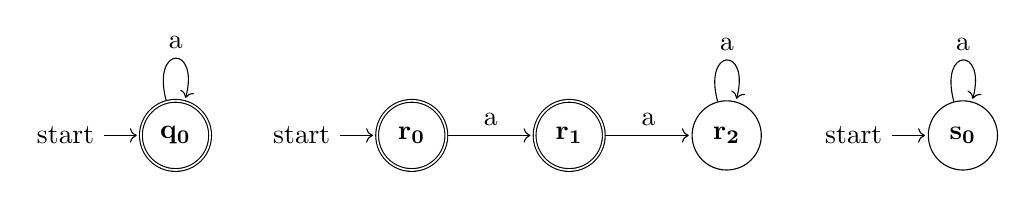
\begin{tikzpicture}[shorten >=1pt,node distance=2cm,on grid,auto,every node/.style={scale=1}]

  \node[initial,state,accepting]  (q_0)                      {$\mathbf{q_0}$};
  \path[->] (q_0) edge [loop above] node {a} ();
  \node [initial, state, accepting] (r_0) [right= 3 cm of q_0] {$\mathbf{r_0}$};
  \node [state,accepting] (r_1) [right= of r_0] {$\mathbf{r_1}$};
  \node [state] (r_2) [right= of r_1] {$\mathbf{r_2}$}; 
  \path[->] (r_0) edge node {a} (r_1);
  \path[->] (r_1) edge node {a} (r_2);
  \path[->] (r_2) edge [loop above] node {a} ();
  \node[initial, state] (s_0) [right= 3 cm of r_2] {$\mathbf{s_0}$};
  \path[->] (s_0) edge [loop above] node {a} ();
\end{tikzpicture}
\]
\caption{Three inequivalent DFAs}	
\label{c2:fig:dfas}
\end{figure*}

Neither of the above automata are language equivalent. Their languages are respectively: $\{\emptyword, a, aa, aaa, \dots\}$, $\{\emptyword, a\}$ and $\emptyset$ (we use $\emptyword$ to denote the empty word). However, one could argue that the behaviour of the middle automaton is closer to the one on the left rather than the one on the right. In particular, languages of the left and middle automaton agree on all words of length less than two, while the left and right one disagree on all words. 

One can make this idea precise, by providing \emph{shortest-distinguishing-word} metric $\langmetric \colon \pset (\alphabet^*) \times \pset (\alphabet^*) \to [0,1]$ on the set of all formal languages over some fixed alphabet $\alphabet$ given by the following formula, where $\lambda \in \interval[open]{0}{1}$ and $L, M \subseteq \alphabet^*$:
\begin{equation}\label{c2:eq:shortest_distinguishing_word}
	d_{\mathcal{L}}(L, M) = \begin{cases}
\lambda^{|w|} & w \text{ is the shortest word that belongs to only one of } L \text{ and } M\\
0 & \text{if } L = M
\end{cases}
\end{equation}

If we set $\lambda = \frac{1}{2}$, then
\begin{gather*}
	\langmetric(\{\emptyword, a, aa, aaa, \dots\}, \{\emptyword, a\}) = \frac{1}{4} \quad \text{ and } \quad \langmetric(\{\emptyword,a,aa,aaa, \dots\}, \emptyset)=1
\end{gather*}
This allows us to formally state that the behaviour of the middle automaton is a better approximation of the left one, rather than the right one. Observe, that we excluded $\lambda=0$ and $\lambda=1$, as in both cases $\langmetric$ would become a pseudometric setting all languages to be at distance zero or one, without providing any quantitative information. 

Rather than dealing with DFAs directly, it has been customary to represent them using the syntax of Kleene's regular expressions~\cite{Kleene:1951:Representation}. For example,  automata depicted in the \Cref{c2:fig:dfas} can be equivalently described using regular expressions $a^*$, $a + 1$ and $0$ respectively.  To determine the distance between arbitrary regular expressions $e$ and $f$ one would have to construct corresponding deterministic finite automata and calculate (or approximate) the distance between their languages. Instead, as a main contribution of this chapter, we present a sound and complete quantitative inference system for reasoning about the shortest-distinguishing-word distance of languages denoted by regular expressions in question.

Since we are dealing with distances, rather than strict equality, we cannot rely on the classical equational logic as a basis for our inference system. Instead, we rely on the quantitative analogue of equational logic~\cite{Mardare:2016:Quantitative}, which deals with the statements of the form $e \equiv_{\e} f$, intuitively meaning \emph{term $e$ is within the distance of at most $\e \in \Q$ from the term $f$}. While the existing work~\cite{Bacci:2018:Algebraic,Bacci:2018:Bisimilarity,Bacci:2018:TV} looked at quantitative axiomatisations of behavioural distance for probabilistic transition systems calculated through the Kantorovich lifting, which can be thought of as a special case of the abstract coalgebraic framework relying on lifting endofunctors to the category of pseudometric spaces~\cite{Baldan:2018:Coalgebraic}, axiomatising behavioural distances for other kinds of transition systems have received little to no attention.

It turns out that the approach to completeness used in~\cite{Bacci:2018:Bisimilarity} relies on properties which are not unique to distances obtained through the Kantorovich lifting and can be employed to give complete axiomatisations of behavioural distances for other kinds of transition systems obtained through the coalgebraic framework~\cite{Baldan:2018:Coalgebraic}. In this chapter, as a starting point, we look at one of the simplest instantiations of that abstract framework in the case of deterministic automata, yielding \emph{shortest-distinguishing-word} distance. 

Formally speaking, if $\sem{-}: \RExp \to \pset (\alphabet^*)$ is a function taking regular expressions to their languages, then our inference system satisfies the following:
$$
	\vdash e \equiv_\e f \iff \langmetric(\llbracket e \rrbracket, \llbracket f \rrbracket) \leq \e
$$ 

The rest of the chapter is organised is as follows:
\begin{itemize}
	\item In \Cref{c2:sec:preliminaries} we review basic definitions from the field of universal coalgebra~\cite{Rutten:2000:Universal,Gumm:2000:Elements} and automata theory. In particular, we recall the semantics of regular expressions through Brzozowski derivatives~\cite{Brzozowski:1964:Expressions}. Then, in order to talk about distances, we state basic definitions and properties surrounding (pseudo)metric spaces.
	\item In \Cref{c2:sec:behavioural_distance} we recall the central notions of the abstract framework of coalgebraic behavioural metrics~\cite{Baldan:2018:Coalgebraic} and discuss its concrete instatiation to the concrete case of deterministic automata that yields shortest-distinguishing-word distance.
	\item In \Cref{c2:sec:quantitative_axiomatisation} we introduce a quantitative inference system for reasoning about the shortest-distinguishing-word distance of regular expressions. We recall the definitions surrounding the quantitative equational theories~\cite{Mardare:2016:Quantitative} from the literature. We then present the rules of our inference system, give soundness result and provide a discussion about the axioms. The interesting insight is that when relying on quantitative equational theories which contain an infinitary rule capturing the notion of convergence, there is no need for any fixpoint introduction rule. We illustrate this by axiomatically deriving Salomaa's fixpoint rule for regular expressions~\cite{Salomaa:1966:Two}.
	\item The key result of our paper is contained in \Cref{c2:sec:completeness}, where we prove completeness of our inference system. The heart of the argument relies on showing that the behavioural distance of regular expressions can be approximated from above using Kleene's fixpoint theorem, which can be then mimicked through the means of axiomatic reasoning. This part of the paper makes heavy use of the order-theoretic and Banach space structures carried by the sets of pseudometrics over a given set.
	\item We conclude in \Cref{c2:sec:discussion}, review related literature, and sketch directions for future work.
\end{itemize}
\section{Preliminaries}\label{c2:sec:preliminaries}
In this section, we recall the main definitions and results from the literature that this and further chapters rely on. Throughout this thesis, we assume the familiarity of the reader with basic notions of category theory~\cite{Abramsky:2010:Introduction} and order theory~\cite{Davey:2002:Introduction}. Notation wise, given a category $\C$, we will write $\Obj(\C)$ for the collection of its objects. For $X,Y \in \Obj(\C)$, we will write $\C(X,Y)$ for the hom-object between objets $X$ and $Y$. We will write $f \colon X \to Y$, to denote that $f$ is a morphism from $X$ to $Y$.
\subsection{Coalgebra}\label{c2:subsec:coalgebra}

Let $\C$ be a category.  An $\funF$-coalgebra is a pair $(X, \alpha \colon X \to \funF X)$, where $X \in \Obj(\C)$ and $\funF \colon \C \to \C$ is an endofunctor on $\C$. We call $\funF$ a \emph{type functor} and refer to $X$ and $\alpha$ as \emph{state space} (or a \emph{carrier}) and \emph{transition structure} respectively. We will omit writing $\funF$ when it is obvious from the context. A homomorphism $f \colon (X, \alpha) \to (Y, \beta)$ of coalgebras is an arrow $f \colon X \to Y$ in $\C$ making the following diagram commute:

% https://q.uiver.app/#q=WzAsNCxbMCwwLCJYIl0sWzAsMSwiXFxmdW5GIFgiXSxbMiwwLCJZIl0sWzIsMSwiXFxmdW5GIFkiXSxbMCwyLCJmIl0sWzIsMywiXFxiZXRhIl0sWzAsMSwiXFxhbHBoYSIsMl0sWzEsMywiXFxmdW5GIGYiLDJdXQ==
\[\begin{tikzcd}
	X && Y \\
	{\funF X} && {\funF Y}
	\arrow["f", from=1-1, to=1-3]
	\arrow["\alpha"', from=1-1, to=2-1]
	\arrow["\beta", from=1-3, to=2-3]
	\arrow["{\funF f}"', from=2-1, to=2-3]
\end{tikzcd}\]
$\funF$-coalgebras and their homomorphisms form a category $\coa{\funF}$. 

\begin{definition}\label{c2:def:final_coalgebra}
We call a coalgebra $(\nu \funF, t)$ \emph{final} if for any coalgebra $(X, \alpha)$, there exists a unique homomorphism $\beh\alpha \colon (X, \alpha) \to (\nu \funF, t)$. A final coalgebra (if it exists) is precisely the final object in $\coa{\funF}$.	
\end{definition}

If $\C$ is a concrete category, that is equipped with a faithful functor $\forget \colon \C \to \Set$, one can define the notion of \emph{behavioural equivalence}. All coalgebras considered in this thesis are defined over concrete categories.
\begin{definition}\label{c2:def:behavioural_equivalence}
Given $\funF$-coalgebras $(X, \alpha)$ and $(Y, \beta)$, and elements $x \in \forget X$, $y \in \forget Y$, we say that $x$ is behaviourally equivalent to $y$ (written $x \beheq y$), if there exists a third coalgebra $(Z, \gamma)$ and $\funF$-coalgebra homomorphisms $f \colon (X, \alpha) \to (Z, \gamma)$ and $g \colon (Y, \beta) \to (Z, \gamma)$, such that $\forget f(x)=\forget g(x)$.	
\end{definition}


For the remainder of this subsection, we will focus on properties of coalgebras for endofunctors over $\Set$ by setting $\funF \colon \Set \to \Set$. For such coalgebras, one can phrase the notion of \emph{coalgebraic bisimulation}.
\begin{definition}\label{c2:def:bisimulation}
Let $(X, \alpha)$ and $(Y, \beta)$ be two coalgebras for the functor $\funF \colon \Set \to \Set$. We call a relation ${R} \subseteq {X \times Y}$ a bisimulation if there exists a transition function $R \to \funF R$ making the following diagram commute:
% https://q.uiver.app/#q=WzAsNixbMCwwLCJYIl0sWzIsMCwiUiJdLFs0LDAsIlkiXSxbMiwxLCJcXGZ1bkYgUiJdLFswLDEsIlxcZnVuRiBYIl0sWzQsMSwiXFxmdW5GIFkiXSxbMCw0LCJcXGFscGhhIl0sWzEsM10sWzIsNSwiXFxiZXRhIl0sWzEsMiwiXFxwaV8yIl0sWzMsNSwiXFxmdW5GIFxccGlfMiIsMl0sWzEsMCwiXFxwaV8xIiwyXSxbMyw0LCJcXGZ1bkYgXFxwaV8xIl1d
\[\begin{tikzcd}
	X && R && Y \\
	{\funF X} && {\funF R} && {\funF Y}
	\arrow["\alpha", from=1-1, to=2-1]
	\arrow["{\pi_1}"', from=1-3, to=1-1]
	\arrow["{\pi_2}", from=1-3, to=1-5]
	\arrow[from=1-3, to=2-3]
	\arrow["\beta", from=1-5, to=2-5]
	\arrow["{\funF \pi_1}", from=2-3, to=2-1]
	\arrow["{\funF \pi_2}"', from=2-3, to=2-5]
\end{tikzcd}\]	
\end{definition}

In the above, $\pi_1 \colon R \to X$ and $\pi_2 \colon R \to Y$ are the canonical projection maps given by the product structure on $X\times Y$. Given $\langle x,y \rangle \in X \times Y$, we write $x \sim y$ if there exists a bisimulation $R$ between $(X, \alpha)$ and $(Y, \gamma)$, such that $\langle x,y \rangle \in R$. Moreover, constructing bisimulations is a sound technique for proving behavioural equivalence. It is also complete upon imposing a mild restriction on $\funF$.
\begin{lemma}[{\cite[Theorem~9.3]{Rutten:2000:Universal}}]\label{c2:lem:behavioural_equivalence}
We have that
$
x \sim y \implies x \beheq y
$. The converse is true if $\funF$ preserves weak pullbacks.	
\end{lemma}
Bisimulations and homomorphisms are related via the following lemma:
\begin{lemma}[{\cite[Theorem~2.5]{Rutten:2000:Universal}}]\label{c2:lem:functional_bisimulation}
	Let $(X, \alpha)$ and $(Y, \beta)$ be two coalgebras. A function $f \colon X \to Y$ is a homomorphism if and only if $G(f) = \{\langle x, f(x) \rangle \mid x \in X\} \subseteq X \times Y$ is a bisimulation.
\end{lemma}
We call a bisimulation that is an equivalence relation a bisimulation equivalence. Forming a quotient using bisimulation equivalences can be used to construct quotient coalgebras.
\begin{lemma}[{\cite[Proposition~5.8]{Rutten:2000:Universal}}]\label{c2:lem:quotient_coalgebra}
	Let $R \subseteq {X \times X}$ be a bisimulation equivalence on a coalgebra $(X, \alpha)$. Let $[-]_{R} \colon X \to {X}/{R}$, be the canonical quotient map of $R$. Then, there is a unique transition structure $\overline{\alpha} \colon {X}/{R} \to \funF {X}/{R}$ on ${X}/{R}$, that makes $[-]_R$ into a coalgebra homomorphism, thus making the following diagram commute:
	 % https://q.uiver.app/#q=WzAsNCxbMCwwLCJYIl0sWzIsMCwie1h9L3tSfSJdLFsyLDEsIlxcZnVuRiB7WH0ve1J9Il0sWzAsMSwiXFxmdW5GIFgiXSxbMCwzLCJcXGFscGhhIl0sWzEsMiwiXFxvdmVybGluZVxcYWxwaGEiXSxbMCwxLCJbLV1fUiJdLFszLDIsIlxcZnVuRiBbLV1fUiIsMl1d
\[\begin{tikzcd}
	X && {{X}/{R}} \\
	{\funF X} && {\funF {X}/{R}}
	\arrow["{[-]_R}", from=1-1, to=1-3]
	\arrow["\alpha", from=1-1, to=2-1]
	\arrow["{\overline\alpha}", from=1-3, to=2-3]
	\arrow["{\funF [-]_R}"', from=2-1, to=2-3]
\end{tikzcd}\]
\end{lemma}
Moreover, one can phrase the dual notion of subalgebras.
\begin{definition}\label{c2:def:subcoalgebra}
A coalgebra $(X, \alpha)$ is called a subcoalgebra of $(Y, \beta)$, if $X \subseteq Y$ and the canonical inclusion map $i \colon X \subto Y$ is a coalgebra homomorphism.	
\end{definition}
Upon imposing a mild restriction on $\funF$, subcoalgebras carry a lattice structure.
\begin{lemma}[{\cite[Theorem~6.4.]{Rutten:2000:Universal}}]\label{c2:lem:subcoalgebras_lattice}
If $\funF$ preserves weak pullbacks, then the collection of all subcoalgebras of a system $(Y, \beta)$ is a complete lattice. Least upper bounds and greatest lower bounds are respectively given by union and intersection of sets. 
\end{lemma}
Given a set $X \subseteq Y$, we will write $\gen{X}{(Y, \beta)}$ for the least subcoalgebra of $(Y, \beta)$ containing $X$.	
In the case when $X$ is a singleton or a two-element set, we will lighten up the notation and respectively write $\gen{x}{(Y, \beta)}$ and $\gen{x,y}{(Y, \beta)}$ instead. Least subcoalgebras allow to characterise an important subcategory of coalgebras.
\begin{definition}\label{c2:def:locally_finite}
We call a coalgebra $(X, \alpha)$ locally finite if for all $x \in X$, we have that $\langle x \rangle_{(X, \alpha)}$ is finite.		
\end{definition}
We will write $\coalf{\funF}$ for the full subcategory of $\coa{\funF}$ consisting only of locally finite coalgebras.
\subsection{Deterministic automata}\label{c2:subsec:deterministic_automata}
A deterministic automaton $\mathcal{M}$ with inputs in a finite alphabet $\alphabet$ is a pair $(M, \langle o_M , t_M \rangle)$ consisting of a set of states $M$ and a pair of functions $\langle o_M, t_M \rangle$, where $o_M \colon M \to \{0,1\}$ is the \emph{output} function which determines whether a state $m$ is final ($o_M(m)=1$) or not ($o_M(m)=0$), and $t :M \to M^\alphabet$ is the \emph{transition} function, which, given an input letter $a$ determines the next state. If the set $M$ of states is finite, then we call an automaton $\mathcal{M}$ a deterministic finite automaton (DFA). We will frequently write $m_a$ to denote $t_M(m)(a)$ and refer to $m_a$ as the derivative of $m$ for the input $a$. Definition of derivatives can be inductively extended to words $w \in \alphabet^{\ast}$. We will write $\emptyword$ to denote an empty word. We set $m_{\emptyword} = m$ and $m_{aw'} = (m_a)_{w'}$ for $a \in \alphabet, w' \in \alphabet^\ast$.
\begin{remark}\label{c2:rem:automata_as_coalgebras}
Note that our definition of deterministic automaton slightly differs from the most common one in the literature, by not explicitly including the initial state. Instead of talking about the language of the automaton, we will talk about the languages of particular states of the automaton. 	
\end{remark}


Given a state $m \in M$, we write $L_{\mathcal{M}} (m) \subseteq {\alphabet^{\ast}}$ for its language, which is formally defined by $L_{\mathcal{M}}(m) = \{w \in \alphabet^\ast \mid o(m_w) = 1\}$. 
Given two deterministic automata $(M, \langle o_M, t_M \rangle)$ and $(N, \langle o_N, t_N \rangle)$, a function $h \colon M \to N$ is a homomorphism if it preserves outputs and input derivatives, that is $o_N(h(m))=o_M(m)$ and $h(m)_a = h(m_a)$. The set of all languages $\pset(\alphabet^{\ast})$ over an alphabet $\alphabet$ can be made into a deterministic automaton $(\pset(\alphabet^\ast), \langle o_L, t_L\rangle)$, where for $l \in \pset (\Sigma^{\ast})$ the output function is given by $o_L(l)=[\emptyword \in l]$ and for all $a \in \alphabet$ the input derivative is defined to be $l_a = \{w \mid aw \in l\}$. This automaton is \emph{final}, that is for any other automaton $\mathcal{M} = (M, \langle o_M, t_M \rangle)$ there exists a unique homomorphism from $M$ to $\pset(\alphabet^{\ast})$, which is given by the map $L_{\mathcal{M}} \colon M \to \pset(\alphabet^\ast)$ taking each state $m \in M$ to its language.
\begin{remark}
	Deterministic automata are precisely coalgebras for the functor $\funDFA \colon \Set \to \Set$ given by $\funDFA = \{0,1\} \times (-)^\alphabet \colon \Set \to \Set$. The coalgebraic definition of homomorphism coincides with the definition of an automaton homomorphism stated above. The final coalgebra for that functor corresponds to the final automaton defined on the set $\pset(\alphabet^\ast)$.
\end{remark}
\subsection{Regular expressions}\label{c2:subsec:regular_expressions}
We let $e, f$ range over \emph{regular expressions over $\alphabet$} generated by the following grammar:
$$e , f \in \RExp ::= \zero \mid \one \mid a \in \alphabet \mid e + f \mid e \seq f \mid e^{\ast}$$
The standard interpretation of regular expressions $\sem{-} \colon \RExp \to \pset(\alphabet^\ast)$ is inductively defined by the following:
\begin{gather*}
	\sem{\zero} = \emptyset \quad \sem{\one} = \{\emptyword\} \quad \sem{a} = \{ a \} \quad \sem{e + f} =  \sem{e}  \cup \sem{f} \\ \sem{e \seq f}  = \sem{e}  \diamond \sem{f} \quad \sem{e^\ast} = \sem{e}^\ast
\end{gather*}
Given $L, M \subseteq A^\ast$, we define $L \diamond M = \{lm \mid l \in L, m \in M\}$, where mere juxtaposition denotes concatenation of words. $L^\ast$ denotes the \emph{asterate} of the language $L$ defined as $L^\ast = \bigcup_{i \in \N} L^i$ with $L^0 = \{\emptyword\}$ and $L^{n + 1} = L \diamond L^{n}$.
\subsection{Brzozowski derivatives}\label{c2:subsec:brzozowski_derivatives}
The famous Kleene's theorem states that the formal languages accepted by DFA are in one-to-one correspondence with formal languages definable by regular expressions. One direction of this theorem involves constructing a \textsf{DFA} for an arbitrary regular expression. The most common way is via Thompson construction, $\emptyword$-transition removal and determinisation. Instead, we recall a direct construction due to Brzozowski~\cite{Brzozowski:1964:Expressions}, in which the set $\RExp$ of regular expressions is equipped with a structure of deterministic automaton $\mathcal{R} = (\RExp, \langle o_{\mathcal{R}}, t_{\mathcal{R}} \rangle)$ through so-called Brzozowski derivatives~\cite{Brzozowski:1964:Expressions}. The output derivative $o_{\mathcal{R}} \colon \RExp \to \{0, 1\}$ is defined inductively by the following 
\begin{gather*}
    o_{\mathcal{R}}(0) = 0 \quad o_{\mathcal{R}}(1) = 1 \quad o_{\mathcal{R}}(a) = 0 \\ o_{\mathcal{R}}(e + f) = o_{\mathcal{R}}(e) \vee o_{\mathcal{R}}(f) \quad
    o_{\mathcal{R}}(e \seq f) = o_{\mathcal{R}}(e) \wedge o_{\mathcal{R}}(f) \quad o_{\mathcal{R}}(e^{\ast}) = 1
\end{gather*}
for $a \in \alphabet$ and $e,f \in \RExp$. Similarly, the transition derivative $t_{\mathcal{R}} \colon \RExp \to \alphabet \to \RExp$ denoted $t_{\mathcal{R}} (e)(a) = (e)_a$ is defined by
\begin{gather*}
    (\zero)_a = 0 \quad (\one)_a = 0 \quad (a')_a = \begin{cases}
        1 & a = a'\\ 0 & a \neq a'  \end{cases}\\
    (e + f)_a = (e)_a + (f)_a \quad
    (e \seq f)_a = (e_a) \seq f + o_{\mathcal{R}}(e) \seq f \quad (e^{\ast}) = (e)_a \seq e^{\ast}
\end{gather*}
Semantics of regular expressions is well-behaved, that is the standard interpretation $\sem{-}$ assigning a language to each regular expression concides with the canonical language-assigning homomorphism from $\mathcal{R}$ to $\mathcal{L}$.
\begin{lemma}[{\cite[Theorem~3.1.4]{Silva:2010:Kleene}}]\label{c2:lem:adequacy}
    For all $e \in \RExp$, $\sem{e} = L_{\mathcal{R}}(e)$
\end{lemma}
Instead of looking at infinite-state automaton defined on the state-space of all regular expressions, we can restrict ourselves to the subautomaton $\gen{e}{\mathcal{R}}$ of $\mathcal{R}$ while obtaining the semantics of $e$.
\begin{lemma}\label{c2:lem:adequacy2}
    For all $e \in \RExp$, $\sem{e} = L_{\gen{e}{\mathcal{R}}}(e)$
\end{lemma}
\begin{proof}
    Let $i \colon \gen{e}{\mathcal{R}} \subto \RExp$ be the canonical inclusion homomorphism. Composing it with $L_{\mathcal{R}}$ a unique homomorphism from $\mathcal{R}$ into the final automaton $\mathcal{L}$ yields a homomorphism $L_{\mathcal{R}} \circ i$ from $\gen{e}{\mathcal{R}}$ to the final automaton, which by finality is the same as $L_{\gen{e}{\mathcal{R}}}$. Using \Cref{c2:lem:adequacy} we can show the following: 
    \[
        \sem{e} = L_{\mathcal{R}}(e)=  L_{\mathcal{R}}(i(e)) = L_{\gen{e}{\mathcal{R}}}(e)
    \]
\end{proof}
Unfortunately, for an arbitrary regular expression $e \in \RExp$, the automaton $\gen{e}{\mathcal{R}}$ is not guaranteed to have a finite set of states. 
However, simplifying the transition derivatives by removing duplicates in the expressions in the form $e_1 + \dots + e_n$, guarantees a finite number of reachable states from any expression. Formally speaking, let ${\acirel} \subseteq {\RExp \times \RExp}$ be the least congruence relation closed under
\begin{enumerate}
	\item $ {{(e + f) + g} {~\acirel~} {e + (f+g)}}$ (Associativity)
	\item ${e + f} {~\acirel~} {f + e}$ (Commutativity)
	\item ${e} {~\acirel~} {e + e}$ (Idempotence) 
\end{enumerate}
	 for all $e,f,g \in \RExp$. 
We will write ${\aciq}$ for the quotient of $\RExp$ by the relation $\acirel$ and $[-]_{\acirel} \colon \RExp \to \aciq$ for the canonical map taking each expression $e \in \RExp$ into its equivalence class $[e]_{\acirel}$ modulo $\acirel$. It can be easily verified that $\acirel$ is a bisimulation and hence using \Cref{c2:lem:quotient_coalgebra}, one can equip $\aciq$ with a structure of deterministic automaton $\mathcal{Q} = (\aciq, \langle o_{\mathcal{Q}}, t_{\mathcal{Q}} \rangle)$, where for all $e \in \RExp, a \in \alphabet$, $o_{\mathcal{Q}}([e]_{\acirel})=o_{\mathcal{R}}(e)$ and $([e]_{\acirel})_a = [e_a]_{\acirel}$, which makes the quotient map $[-]_{\acirel} \colon \RExp 
\to \aciq$ into an automaton homomorphism from the Brzozowski automaton $\mathcal{R}$ into $\mathcal{Q}$. This automaton enjoys the following property:
\begin{lemma}[{\cite[Theorem~4.3]{Brzozowski:1964:Expressions}}]\label{c2:lem:locally_finite}
    For any $e \in \RExp$, the set $\gen{e}{\mathcal{Q}} \subseteq \aciq$ is finite.
\end{lemma}
Through the identical line of reasoning to \Cref{c2:lem:adequacy}, we can show that:
\begin{lemma}
	For all $e \in \RExp$, $L_{\gen{[e]_{\acirel}}{\mathcal{Q}}}([e]_{\acirel}) = \sem{e}$
\end{lemma}
\subsection{Pseudometric spaces}\label{c2:subsec:pseudometric_spaces}
A $1$-bounded \emph{pseudometric} on a set $X$ (or equivalently just a \emph{pseudometric}) is a function $d \colon X \times X \to \interval{0}{1}$ satisfying
\begin{enumerate}
	\item  $d(x,x)=0$ (Reflexivity)
	\item  $d(x,y)=d(y,x)$ ({Symmetry})
	\item  $d(x,z) \leq d(x, y) + d(y,z)$ (Triangle inequality)
\end{enumerate}
for all $x,y,z \in X$. If additionally $d(x,y)=0$ implies $x=y$, $d$ is called a ($1$-bounded) \emph{metric}. 
\begin{definition}
	A pseudometric space is a pair $(X, d)$, where $X$ is a set and $d$ is a pseudometric on $X$. We call a function $f \colon X \to Y$ between pseudometric spaces $(X,d_1)$ and $(Y,d_2)$ nonexpansive, if $d_2(f(x),f(y))\leq d_1(x,y)$ for all $x,y \in X$. It is called isometry if it satisfies $d_Y(f(x),f(y))=d_X(x,y)$. 	
\end{definition}
Pseudometrics and nonexpansive functions form a category $\PMet$. This category is bicomplete, i.e. has all limits and colimits~\cite[Theorem~3.8]{Baldan:2018:Coalgebraic}. The categorical product in $\PMet$ is defined via the following:
\begin{definition}
Let $(X,d_1)$ and $(Y, d_2)$ be pseudometrics. We define $(X, d_1) \times (Y, d_2) = (X \times Y, d_{X \times Y})$, where $d_{X \times Y}(\langle x,y \rangle,\langle x',y' \rangle ) = \max \{d_1(x,x'), d_2(y,y')\}$ for all $x,x' \in X$ and $y,y' \in Y$.
\end{definition}
This can be easily extended to any $n$-tuple. We define $0$-tuples to be given by $1_{\bullet} = (\{\bullet\}, d_{\bullet})$, the unique single point pseudometric space, where $d_{\bullet}(\bullet,\bullet)=0$. Given a function of multiple arguments, i.e. $X_1 \to X_2 \to Y$, we will call it nonexpansive, if it is nonexpansive as a function $f \colon (X_1, d_{1}) \times (X_2, d_{2}) \to (Y, d_Y)$. 	


Given a set $X$, we write $D_X$ for the set of all pseudometrics on the set $X$. This set carries a partial order structure, given by
$$d_1 \sqsubseteq d_2 \iff \forall x,y \in X \ldotp d_1(x,y) \leq d_2(x,y)$$  
\begin{lemma}[{\cite[Lemma~3.2]{Baldan:2018:Coalgebraic}}]\label{c2:lem:pseudometrics_complete_lattice}
    $(D_X, \sqsubseteq )$ is a complete lattice. The join of an arbitrary set of pseudometrics $D \subseteq D_X$ is taken pointwise, ie. $\left(\sup D \right)(x,y) = \sup \{ d(x,y) \mid d \in D\}$ for $x, y \in X$. The meet of $D$ is defined to be $\inf D = \sup \{ d \mid d \in D_X , \forall {d' \in D}, d \sqsubseteq d'\}$.
\end{lemma}
The top element of that lattice is given by the discrete pseudometric $\top \colon X \times X \to [0,1]$ such that $\top(x,y) = 0$ if $x=y$, or $\top(x,y)=1$ otherwise.

Crucially for our completeness proof, if we are dealing with descending chains, that is sequences $\{d_i\}_{i \in \N}$, such that $d_i \sqsupseteq d_{i+1}$ for all $i \in \N$, then we can also calculate infima in the pointwise way.
\begin{lemma}\label{c2:lem:chain_pointwise_inf}
    Let $\{d_i\}_{i \in \N}$ be an infinite descending chain in the lattice $(D_X, \sqsubseteq)$ of pseudometrics over some fixed set $X$. Then $(\inf\{d_i \mid i \in \N\})(x,y) = \inf \{d_i(x,y) \mid i \in \N \}$ for any $x,y \in X$.
\end{lemma}
\begin{proof}
    It suffices to argue that $d(x,y) = \inf \{d_i(x,y) \mid i \in \N \}$ is a pseudometric. For reflexivity, observe that $d(x,x) = \inf \{d_i(x,x) \mid i \in \N \} = \inf \{ 0 \} = 0 $ for all $x \in X$. 
    
    For symmetry, we have that $d(x,y) = \inf \{d_i(x,y) \mid i \in \N \} =  \inf \{d_i(y,x) \mid i \in \N \}=d(y,x)$ for any $x, y \in X$. 
    
    The only difficult case is triangle inequality. First, let $i, j \in \N$ and define $k = \max(i,j)$. Since $d_k \sqsubseteq d_i$ and $d_k \sqsubseteq d_j$, we have that $d_k(x,y) + d_k(y,z) \leq d_i(x,y) + d_j(y,z)$.
    Therefore $\inf \{d_l(x,y) + d_l(y,z) \mid l \in \N\}$ is a lower bound of $d_i(x,y) + d_j(y,z)$ for any $i, j \in \N$ and hence it is below the greatest lower bound, that is $\inf \{d_l(x,y) + d_l(y,z) \mid l \in \N\} \leq \inf \{d_i(x,y) + d_j(y,z) \mid i,j \in \N\}$. We can use that property to show that
    \begin{align*}
    	d(x,y) &= \inf \{d_i(z,y) \mid i \in \N\} \\
    	&\leq \inf \{d_i(x,y) + d_i(y,z) \mid i \in \N\}\\
    	&\leq \inf \{d_i(x,y) + d_j(y,z) \mid i,j \in \N\}\\
    	&= \inf \{d_i(x,y) \mid i \in \N\} + \inf \{d_j(y,z) \mid j \in \N\}\\
    	&= d(x,y) + d(y,z)
    \end{align*}
	which completes the proof.
\end{proof}
Additionally, the set of pseudometrics can be equipped with a norm. We write $\eR = [-\infty, \infty]$ for the set of extended reals. For any set $X$, the set of functions $\eR^{X \times X }$, which is a superset of $D_X$, can be seen as a Banach space~\cite{Rudin:1990:Functional} (complete normed vector space) by means of the sup-norm $\|d\| = \sup_{x,y \in X} |d(x,y)|$. This structure will implicitly underly some of the claims used as intermediate steps in the proof of completeness in this and next chapter.
\section{Behavioural distance}\label{c2:sec:behavioural_distance}
We now move on to defining behavioural distance for deterministic automata through the abstract framework of coalgebraic behavioural distances~\cite{Baldan:2018:Coalgebraic}. We first recall the main definitions and then concretise the abstract results to the case of our interest.
\subsection{Coalgebraic behavioural distances}\label{c2:subsec:coalgebraic_behavioural_distances}
In order to define a behavioural distance for $\funF$-coalgebras for a functor $\funF \colon \Set \to \Set$, we need to be able to \emph{lift} the functor $\funF$ describing the one-step dynamics of transition systems of interest to the category $\PMet$ of pseudometric spaces and nonexpansive functions. In terms of notation, we will write $\forget \colon \PMet \to \Set$ for the canonical faithful functor taking each pseudometric space $(X, d_X)$ to its underlying set $X$.
\begin{definition}\label{c2:def:lifting}
	Let $\funF \colon \Set \to \Set$ be a functor. We call a functor $\overline{\funF} \colon \PMet \to \PMet$ a lifting of $\funF$ if makes the following diagram commute:
	% https://q.uiver.app/#q=WzAsNCxbMCwwLCJcXFBNZXQiXSxbMSwwLCJcXFBNZXQiXSxbMCwxLCJcXFNldCJdLFsxLDEsIlxcU2V0Il0sWzAsMSwiXFxvdmVybGluZXtcXGZ1bkZ9Il0sWzIsMywiXFxmdW5GIl0sWzEsMywiXFxmb3JnZXQiXSxbMCwyLCJcXGZvcmdldCIsMl1d
\[\begin{tikzcd}
	\PMet & \PMet \\
	\Set & \Set
	\arrow["{\overline{\funF}}", from=1-1, to=1-2]
	\arrow["\forget"', from=1-1, to=2-1]
	\arrow["\forget", from=1-2, to=2-2]
	\arrow["\funF", from=2-1, to=2-2]
\end{tikzcd}\]
Given a pseudometric space $(X, d)$, we will write $d^{\funF}$ for the pseudometric $d^{\funF} \colon \funF X \times \funF X \to \interval{0}{1}$ obtained by applying $\overline{\funF}$ to $(X,d)$.
\end{definition}
We can use liftings to equip coalgebras with a notion of behavioural distance, through the following construction:
\begin{lemma}[{\cite[Lemma~6.1]{Baldan:2018:Coalgebraic}}]\label{c2:lem:behavioural_distances}
	Let $\overline{\funF} \colon \PMet \to \PMet$ be a lifting of a functor $\funF \colon \Set \to \Set$ and let $(X, \alpha)$ be a $\funF$-coalgebra. The mapping associating each pseudometric $d \colon X \times X \to [0,\top]$ with $d^{\funF} \circ (\alpha \times \alpha)$ is a monotone mapping on the complete lattice $(D_X, \sqsubseteq)$ of pseudometrics over set $X$. By Knaster-Tarski fixpoint theorem, this mapping has a least fixpoint, that we will refer to as $d_\alpha \colon X \times X \to \interval{0}{1}$. Given a coalgebra $(Y, \beta)$ and a homomorphism $f \colon (X, \alpha) \to (Y, \beta)$, we have that $f \colon (X, d_\alpha) \to (Y, d_\beta)$ is nonexpansive. If $\overline{\funF}$ preserves isometries, then $f$ is an isometry.
\end{lemma}
If $\funF \colon \Set \to \Set$ admits a final coalgebra $(\nu \funF, t)$, then we can define behavioural distance on a  coalgebra $(X, \alpha)$ to be the pseudometric space $\bd_\alpha \colon X\times X \to \interval{0}{1}$ given by $\bd_\alpha(x,y) = d_{t}(\beh{\alpha}(x), \beh{\alpha}(y))$ for all $x, y \in X$. Behavioural distances satisfy several desirable properties:
\begin{lemma}\label{c2:lem:behavioural_distances_properties}
	Let $\overline{\funF} \colon \PMet \to \PMet$ be a lifting of a functor $\funF \colon \Set \to \Set$ that admits a final coalgebra $(\nu \funF, t)$. Given a coalgebra $(X, \alpha)$ and $x,y \in X$, the following facts hold:
	\begin{enumerate}
		\item $x \beheq y \implies \bd_\alpha(x,y)=0$
		\item If $\overline\funF$ preserves metrics and $\funF$ is finitary, then $\bd_\alpha(x,y)=0 \implies x \beheq y$
		\item If $\overline{\funF}$ preserves isometries, then $d_\alpha(x,y) = \bd(x,y)$
	\end{enumerate}
\end{lemma}
\begin{proof}
	\circlednum{1} follows from \cite[Lemma~6.6]{Baldan:2018:Coalgebraic}. For \circlednum{2}, we have that if $\funF$ is finitary, then $(\nu \funF,t)$ can be obtained via the Adamek fixpoint theorem~\cite{Adamek:1995:Greatest} and hence one can apply \cite[Theorem~6.10]{Baldan:2018:Coalgebraic}. Finally, \circlednum{3} follows from \cite[Theorem~6.7]{Baldan:2018:Coalgebraic}.
\end{proof}
\subsection{Behavioural distance of deterministic automata via functor lifting}	
It turns out that shortest-distinguishing-word distance can be obtained as an instance of the coalgebraic framework of behavioural distances~\cite[Example~6.5]{Baldan:2018:Coalgebraic} using an appropriate lifting of the functor $\funDFA = \{0,1\} \times (-)^\alphabet$ describing one-step behaviour of finite automata~\cite[Example~6.3]{Baldan:2018:Coalgebraic}. That lifting is defined as follows; let $d \colon M \times M \to [0,1]$ be a pseudometric and let $\lambda \in \interval[open]{0}{1}$ be a fixed \emph{discount factor}. We can equip the set $\funDFA X$ with a distance function given by
\[
	d^{\funDFA}(\langle o_1, g_1 \rangle, \langle o_2, g_2 \rangle) = \max\{d_{\{0,1\}}(o_1, o_2), \lambda \cdot \max_{a \in \alphabet} d(g_1(a), g_2(a))\} 
\]   
for all $\langle o_1, g_1 \rangle, \langle o_2, g_2 \rangle \in \funDFA X$. The definition above involves $d_{\{0,1\}}$, the discrete metric on the set $\{0,1\}$. Intuitively, two one-step behaviours $\langle o_1, g_1\rangle, \langle o_2, g_2 \rangle \in \{0,1\} \times M^\alphabet$ of a deterministic automaton with the set of states $M$ are maximally apart if $o_1 \neq o_2$, that is, they disagree in their output behaviour. Otherwise, the distance is equal to a maximal distance $d(g_1(a), g_2(a))$ between reachable states for all letters $a \in \alphabet$ of the alphabet, discounted by the factor of $\lambda$.

The lifting defined above is particularly well-behaved, as it satisfies the following:

\begin{proposition}
	$d^{\funDFA}$ preserves isometries and metrics.
\end{proposition}
\begin{proof}
	Preservation of isometries follows from \cite[Theorem 5.23]{Baldan:2018:Coalgebraic} and preservation of metrics follows from~\cite[Theorem~5.24]{Baldan:2018:Coalgebraic}.
\end{proof}
Combining the statement above with \Cref{c2:lem:behavioural_distances} and \Cref{c2:lem:behavioural_distances_properties} yields that for any deterministic automaton $\mathcal{M} := (M, \langle o_M, t_M \rangle)$, its behavioural distance $\bd_{\langle o_M, t_M \rangle}$ is a metric space, whose values can be calculated as the least fixpoint of the monotone map $\Phi_{\langle o_M, t_M\rangle} \colon D_M \to D_M$ defined as
$$
\Phi_{\langle o_M, t_M\rangle}(m_1, m_2) = d^{\funDFA}(\langle o_M(m_1), t_{M}(m_1) \rangle, \langle o_M(m_2), t_{M}(m_2) \rangle)
$$
for all $m_1, m_2 \in M$.

\section{Quantitative Axiomatisation}\label{c2:sec:quantitative_axiomatisation}
In order to provide a quantitative inference system for reasoning about the behavioural distance of languages denoted by regular expressions, we first recall the definition of quantitative equational theories from the existing literature~\cite{Mardare:2016:Quantitative,Bacci:2018:Bisimilarity} following the notational conventions from~\cite{Bacci:2018:Bisimilarity}. We then present our axiomatisation and demonstrate its soundness. The interesting thing about our axiomatisation is the lack of any fixpoint introduction rule. We show that in the case of quantitative analogue of equational logic~\cite{Mardare:2016:Quantitative} containing the infinitary rule capturing the notion of convergence, we can use our axioms to derive Salomaa's fixpoint rule from his axiomatisation of language equivalence of regular expressions~\cite{Salomaa:1966:Two}.

\subsection{Quantitative equational theories}\label{c2:subsec:quantitative_equational_theories} 
Let $\Sigma$ be an algebraic signature (in the sense of universal algebra~\cite{Burris:1981:Course}) consisting of operation symbols $f_n \in \Sigma$ of arity $n \in \N$. If we write $X$ for the countable set of \emph{metavariables}, then $\TT[\Sigma]{X}$ denotes a set of freely generated terms over $X$ built from the signature $\Sigma$. As a notational convention, we will use letters $t,s,u, \ldots \in \TT[\Sigma]{X}$ to denote terms. 
By a \emph{substitution} we mean a function of the type $\sigma\colon X \to \TT[\Sigma]{X}$ allowing to replace metavariables with terms. Each substitution can be inductively extended to terms in a unique way by setting $\sigma(f(t_1, \dots, t_n)) = f(\sigma(t_1), \dots, \sigma(t_n))$ for each operation symbol $f_n \in \Sigma$ from the signature. We will write $\Sub[\Sigma]$ for the set of all substitutions. Given two terms $t,s \in \TT[\Sigma]{X}$ and a nonnegative rational number $\e \in \Q$ denoting the distance between the terms, we call $t \equiv_\e s$ a \emph{quantitative equation (of type $\Sigma$)}. Notation-wise, we will write $\E[\Sigma]$ to denote the set of all quantitative equations (of type $\Sigma$) and we will use the capital Greek letters $\Gamma, \Theta, \ldots \subseteq \E[\Sigma]$ to denote the subsets of $\E[\Sigma]$. By a \emph{deducibility relation} we mean a binary relation denoted  ${\vdash} \subseteq \pset ({\E[\Sigma]}) \times \E[\Sigma]$.  Similarly, to the classical equational logic, we will use the following notational shorthands:
\begin{gather*} 
	\Gamma \vdash t \equiv_\e s \iff (\Gamma,t \equiv_\e s) \in {\vdash} \qquad \text{ and } \qquad \vdash t \equiv_\e s \iff \emptyset \vdash t \equiv_\e s
\end{gather*}
Furthermore, following the usual notational conventions, we will write $\Gamma \vdash \Theta$ as a shorthand for the situation when $\Gamma \vdash t \equiv_\e s$ holds for all $t \equiv_\e s \in \Theta$. To call $\vdash$ a \emph{quantitative deduction 
system (of type $\Sigma$)} it needs to satisfy the following rules of inference: 
\begin{align*} 
(\Top) \quad 
& \vdash t \equiv_1 t \,, \\
(\Refl) \quad 
& \vdash t \equiv_0 t \,, \\
(\Symm) \quad 
& \{t\equiv_\e s\} \vdash s\equiv_\e t \,, \\
(\Triang) \quad 
& \{t \equiv_\e u, u \equiv_{\e'} s \} \vdash t \equiv_{\e+\e'} s \,, \\
(\Max) \quad 
& \{t\equiv_\e s\} \vdash t\equiv_{\e+\e'}s \,, \text{ for all $\e'>0$} \,, \\ 
(\Cont) \quad 
& \{t\equiv_{\e'}s\mid \e'>\e\} \vdash t\equiv_\e s \,, \\
(\Nexp) \quad
& \{t_1\equiv_\e s_1,\ldots,t_n \equiv_\e s_n\} \vdash f(t_1,\dots, t_n) \equiv_\e f(s_1,\dots, s_n) \,, 
\text{ for all $f_n \in \Sigma$} \,, \\
(\Subst) \quad
& \text{If $\Gamma \vdash t \equiv_\e s$, then $\sigma(\Gamma) \vdash \sigma(t) \equiv_\e \sigma(s)$, 
for all $\sigma \in \Sub[\Sigma]$} \,, \\
(\Cut) \quad 
& \text{If $\Gamma \vdash \Theta$ and $\Theta \vdash t \equiv_\e s$, then $\Gamma \vdash t \equiv_\e s$} \,, \\
(\Assum) \quad
& \text{If $t \equiv_\e s \in\Gamma$, then $\Gamma \vdash t \equiv_\e s$} \,.
\end{align*}
where $\sigma(\Gamma) = \set{\sigma(t) \equiv_\e \sigma(s)}{ t \equiv_\e s \in \Gamma}$.
Finally, by a \emph{quantitative equational theory} we mean a set $\U$ of universally quantified \emph{quantitative inferences} 
$
\{t_1 \equiv_{\e_1} s_1, \dots, t_n \equiv_{\e_n} s_n\} \vdash t \equiv_\e s \,,
$ with \emph{finitely many premises}, closed under $\vdash$-derivability.

\subsection{Quantitative algebras}\label{s2:subsec:quantitative_algebras} 

Quantitative equational theories lie on the syntactic part of the picture. On the semantic side, we have their models called \emph{quantitative algebras}, defined as follows. 

\begin{definition}[{\cite[Definition~3.1]{Mardare:2016:Quantitative}}]
    A quantitative algebra is a tuple $\qalgA = (A, \Sigma^{\qalgA}, d^{\qalgA})$, such that $(A, \Sigma^{\qalgA})$ is an algebra for the signature $\Sigma$ and $(A, d^{\qalgA})$ is a pseudometric such that for all operation symbols $f_n \in \Sigma$, for all $1 \leq i \leq n$, $a_i, b_i \in \alphabet$, $d^{\qalgA}(a_i,b_i)\leq \e$ implies $d^{\qalgA}(f^{\qalgA}(a_1, \dots, a_n), f^{\qalgA}(b_1, \dots, b_n)) \leq \e$.
\end{definition}

Consider a quantitative algebra $\qalgA = (A,\Sigma^\qalgA,d^\qalgA)$. Given an assignment  $\iota \colon X \to A$ of meta-variables from $X$ to elements of carrier $A$, one can inductively extend it to $\Sigma$-terms $t \in \TT[\Sigma]{X}$ in a unique way. We will abuse the notation and just write $\iota(t)$ for the interpretation of the term $t$ in quantitative algebra $\qalgA$. We will say that $\qalgA$ \emph{satisfies} the quantitative inference $\Gamma \vdash t \equiv_\e s$, written $\Gamma \models_\qalgA t \equiv_\e s$, if for any assignment of the meta-variables $\iota \colon X \to A$ it is the case that for all $t' \equiv_{\e'} s' \in \Gamma$ we have that $d^\qalgA(\iota(t'),\iota(s')) \leq \e'$ implies $d^\qalgA(\iota(t),\iota(s)) \leq \e $. Finally, we say that a quantitative algebra $\qalgA$ \emph{satisfies} (or is a \emph{model} of) the quantitative theory $\U[]$, 
if whenever $\Gamma \vdash t \equiv_\e s \in \U[]$, then $\Gamma \models_\qalgA t \equiv_\e s$. 

\subsection{Quantitative algebra of regular expressions}\label{c2:subsec:quantitative_algebra_of_regular_expressions}

From now on, let's focus on the signature $\Sigma^{\qalgB} = \{\zero_0, \one_0, +_2, \seq_2, {(-)^\ast}_1\} \cup \{a_0 \mid a \in \alphabet\}$, where $\alphabet$ is a finite alphabet. This signature consists of all operations of regular expressions. We can easily interpret all those operations in the set $\RExp$ of all regular expressions, using trivial interpretation functions eg. $+^{\qalgB}(e,f) = e + f$, which interpret the operations by simply constructing the appropriate terms. Formally speaking, we can do this because the set $\RExp$ is the carrier of initial algebra~\cite{Burris:1981:Course} (free algebra over the empty set of generators) for the signature $\Sigma$. 

To make this algebra into a quantitative algebra, we first equip the set $\RExp$ with a pseudometric, given by $
d^{\qalgB}(e,f) = \langmetric(\sem{e}, \sem{f})$ for all $e, f \in \RExp$. 

Recall that $\langmetric$ used in the definition above is a behavioural pseudometric on the final deterministic automaton carried by the set $\pset (\alphabet^{\ast})$ of all formal languages over an alphabet $\alphabet$. In other words, we define the distance between arbitrary expressions $e$ and $f$ to be the distance between formal languages $\sem{e}$ and $\sem{f}$ calculated through the shortest-distinguishing-word metric. 
It turns out, that in such a situation all the interpretation functions of $\Sigma$-algebra structure on $\RExp$ are nonexpansive with respect to the pseudometric defined above. In other words, we have that: 

\begin{lemma}\label{c2:lem:quantitative_algebra}
    $\qalgB = (\RExp, \Sigma^{\qalgB}, d^{\qalgB})$ is a quantitative algebra.
\end{lemma}
\begin{proof}
Since $\langmetric$ is a pseudometric, then so is $d^{\qalgB} = \langmetric \circ (\sem{-}\times\sem{-})$. We now verify the nonexpansivity of interpretations of operations with non-zero arity. Let $e,f,g,h \in \RExp$, $d^{\qalgB}(e,g) \leq \e$ and $d^{\qalgB}(f,h) \leq \e$. 

\begin{enumerate}
    \item We show that $d^{\qalgB}(e + f, g + h) \leq \e$. In the case when $\e = 0$, the proof simplifies to showing that if $\sem{e} = \sem{g}$ and $\sem{f} = \sem{h}$ then $\sem{e + g} = \sem{g + h}$, which holds immediately. 
    For the remaining case, when $\e > 0$, let $n = \lceil \log_{\lambda} \e \rceil$. 
    
    Observe that in such a case, we have that $d^{\qalgB}(e,g) \leq \lambda^n$ and $d^{\qalgB}(f,h) \leq \lambda^n$. Using it, we can deduce that $\sem{e}$ and $\sem{g}$ (and similarly $\sem{f}$ and $\sem{h}$) agree on all words of length strictly below $n$ (because the shortest word for which they disagree is at least of length $n$). To put that formally:
    $$\forall w \in \alphabet^{\ast} \ldotp |w| < n \implies \left(w \in \sem{e} \iff w \in \sem{g} \right) \wedge  \left(w \in \sem{f} \iff w \in \sem{h} \right) $$
    Let $w \in \alphabet^\ast$, such that $|w|<n$. We have that 
    \begin{align*}
        w \in \sem{e + f} &\iff w \in \sem{e} \cup \sem{f} \iff \left(w \in \sem {e}\right) \vee \left(w \in \sem{f}\right) \\
        &\iff \left(w \in \sem{g}\right) \vee \left(w \in \sem{h}\right) \tag{$|w| < n$} \\
        &\iff w \in \sem{g + h}
    \end{align*}
    And thus $\sem{e + f}$ and $\sem{g + h}$ agree on all words of the length below $n$ and therefore $d^{\qalgB}(e + f, g + h) \leq \lambda^{n} \leq \e$.
    
    \item The case for $\e = 0$ holds immediately through the same line of reasoning as before, relying on well-definedness of $\diamond$ (concatenation) operation on formal languages. We focus on the remaining case, making the same simplification as before, that is we assume that $\sem{e}$ and $\sem{g}$ (as well as $\sem{f}$ and $\sem{h}$) agree on all word of length strictly below $n$). We show that $\sem{e \seq f}$ and $\sem{g \seq h}$ also agree on all words of the length strictly less than $n$. Let $w \in \alphabet^{\ast}$, such that $|w|<n$. We have that: 
    \begin{align*}
        w \in \sem{e \seq f} &\iff w \in \sem{e} \diamond \sem{f}\\ &\iff
        \left(\exists u,v \in \alphabet^\ast \ldotp w=uv \wedge w \in \sem{e} \wedge v \in \sem{f}\right)\\
        &\iff  \left(\exists u,v \in \alphabet^\ast \ldotp w=uv \wedge w \in \sem{g} \wedge v \in \sem{h}\right) \tag{ $|u|< n$ and $|v| < n$} \\
        &\iff w \in \sem{g} \diamond \sem{h} \iff w \in \sem {g \seq h}
    \end{align*}
    \item We use the same line of reasoning as before. Assume that $\sem{e}$ and $\sem{g}$ agree on all words of length below $n$. Let $w \in \alphabet^\ast$, such that $|w| < n$. We have the following:
    \begin{align*}
        w \in \sem{e^\ast} &\iff w \in \sem{e}^\ast\\ 
        &\iff w = \e \vee \left(\exists k \geq 1 \ldotp \exists u_1, \dots, u_k \in \alphabet^\ast \ldotp w = u_1\dots u_k \right.\\&\left. \qquad\qquad\wedge u_1 \in \sem{e} \wedge \dots \wedge u_k \in \sem{e}\right) \\
        &\iff w = \e \vee \left(\exists k \geq 1 \ldotp \exists u_1, \dots, u_k \in \alphabet^\ast\ldotp w = u_1\dots u_k \right.\\&\left. \qquad\qquad\wedge u_1 \in \sem{g} \wedge \dots \wedge u_k \in \sem{g}\right) \tag{$|u_1| < n, \dots, |u_k| < n$ }\\
        &\iff w \in \sem{g}^\ast \iff w \in \sem{g^*}
    \end{align*}
\end{enumerate}
\end{proof}
In order to talk about the quantitative algebra $\qalgB$ of the behavioural distance of regular expressions in an axiomatic way, we introduce the quantitative equational theory \textsf{REG} (\Cref{c2:fig:axioms}).

\begin{figure}[h]
	
{
\small
\begin{tabular}{l@{\quad}l}
\(
\begin{array}{ll}
&\textbf{Nondeterministic choice}\\
(\mathsf{SL1})\;\; 
& \vdash e + e \equiv_0 e \,, \\
(\mathsf{SL2})\;\; 
& \vdash e + f \equiv_0 f + e \,, \\
(\mathsf{SL3})\;\; 
& \vdash (e + f) + g\equiv_0 e + (f + g) \,, \\
(\mathsf{SL4})\;\; 
& \vdash e + \zero\equiv_0 e \,, \\
(\mathsf{SL5})\;\; & \{ e \equiv_\e g , f \equiv_{\e'} h\} \\ & \quad\vdash e + f \equiv_{\max(\e, \e')} g + h \,, \\\\\\
%% recursion
&\textbf{Loops} \\
(\mathsf{Unroll})\;\; & \vdash e^\ast \equiv_0 e \seq e^{\ast} + 1 \,, \\
(\mathsf{Tight})\;\; & \vdash (e + \one)^\ast \equiv_0 e^\ast \,, \\[1.2ex]
%%(\Fix)\;\; & \{ s \equiv_0 t[s / X] \} \vdash s \equiv_0 \rec{X}{t} \,, \text{ for $X$ guarded in $t$} \,, \\
%% distance
\end{array}
\)&
\(
\begin{array}{ll}
&\textbf{Sequential composition}\\
	(\mathsf{1S})\;\; 
& \vdash \one \seq e \equiv_0 e \,, \\
(\mathsf{S})\;\; 
& \vdash e \seq (f \seq g) \equiv_0 (e \seq f) \seq g \,, \\
(\mathsf{S1})\;\; 
& \vdash e \seq \one \equiv_0 e \,, \\
(\mathsf{0S})\;\; 
& \vdash \zero \seq e \equiv_0 \zero \,, \\
(\mathsf{S0})\;\; 
& \vdash e \seq \zero \equiv_0 \zero \,, \\
(\mathsf{D1})\;\; 
& \vdash e \seq (f + g) \equiv_0 e \seq f + e \seq g \,, \\
(\mathsf{D2})\;\; 
& \vdash (e + f) \seq g \equiv_0 e \seq g + f \seq g \,, \\\\
&\textbf{Behavioural pseudometric}\\
(\dPref)\;\; & \{ e \equiv_\e f \} \vdash a \seq e \equiv_{\e'} a \seq f \,,\\&\qquad \text{for $\e'\geq \lambda \cdot \e$} \\[1.2ex]
\end{array}
\)
\end{tabular}
}	
\caption{Axioms of the quantitative equational theory \textsf{REG} for $e,f,g \in \RExp$ and $a \in \alphabet$.}
\label{c2:fig:axioms}
\end{figure}

The first group of axioms capture properties of the nondeterministic choice operator $+$ \textsf{(SL1-SL5)}. The first four axioms \textsf{(SL1-SL4)} are the usual laws of semilattices with bottom element $\zero$. (\textsf{SL5}) is a quantitative axiom allowing one to reason about distances between sums of expressions in terms of distances between expressions being summed. Moreover, \textsf{(SL1-SL5)} are axioms of so-called \emph{Quantitative Semilattices with zero}, which have been shown to axiomatise the Hausdorff metric~\cite{Mardare:2016:Quantitative}. 

The sequencing axioms \textsf{(1S), (S1), (S)} state that the set $\RExp$ of regular expressions has the structure of a monoid (with neutral element $\one$) with absorbent element $0$ \textsf{(0S), (S0)}. Additionally, \textsf{(D1-D2)} talk about interaction of the nondeterministic choice operator $+$ with sequential composition. 

The loop axioms \textsf{(Unroll)} and \textsf{(Tight)} are directly inherited from Salomaa's axiomatisation of language equivalence of regular expressions~\cite{Salomaa:1966:Two}. \textsf{(Unroll)} axiom associates loops with their intuitive behaviour of choosing, at each step, between successful termination and executing the loop body once. \textsf{(Tight)} states that the loop whose body might instantly terminate, causing the next loop iteration to be executed immediately is provably equivalent to a different loop, whose body does not contain immediate termination. 
%Contrary to Salomaa~\cite{Salomaa:1966:Two} and Kozen~\cite{Kozen:1994:Completeness} we do not include any fixpoint rule allowing the introduction of loops. We will elaborate on this in the next section, showing that in the presence of infinitary \textsf{(Cont)} rule of the quantitative deduction systems, Salomaa's rule for introducing loops is derivable from other axioms of \textsf{REG}. 
Finally, \textsf{(\dPref)} captures the fact that prepending the same letter to arbitrary expressions shrinks the distance between them by the factor of $\lambda \in \interval[open]{0}{1}$ (used in the definition of $d^{\qalgB}$). This axiom is adapted from the axiomatisation of discounted probabilistic bisimilarity distance~\cite{Bacci:2018:Bisimilarity}.
Through a simple induction on the length of derivation, one can verify that indeed $\qalgB$ is a model of the quantitative theory \textsf{REG}. 
\begin{theorem}[Soundness]\label{c2:thm:soundness}
    The quantitative algebra $\qalgB = (\RExp, \Sigma^{\qalgB}, d^\qalgB)$ is a model of the quantitative theory $\mathsf{REG}$. In other words, for any $e, f \in \RExp$ and $\e \in \Q$, if $\Gamma \vdash e \equiv_\e f \in \mathsf{REG}$, then $\Gamma \models_\qalgB e \equiv_\e f$
\end{theorem}
\begin{proof}
By the structural induction on the judgement $\Gamma \vdash e \equiv_{\e} f \in \mathsf{REG}$. $(\Subst)$, $(\Cut)$ and $(\Assum)$ deduction rules from classical logic hold immediately. The soundness of $(\Top)$, $(\Refl)$, $(\Symm)$, $(\Triang)$, $(\Cont)$ and $(\Max)$ follows from the fact that $d^{\qalgB}$ is a pseudometric. $(\Nexp)$ follows from the fact that interpretations of symbols from the algebraic signature are nonexpansive (\cref{c2:lem:quantitative_algebra}). Recall that $d^{\qalgB} = \langmetric \circ (\sem{-} \times \sem {-})$. 

 Additionally, for all axioms in the form $\vdash e \equiv_0 f$ it suffices to show that $\sem{e} = \sem{f}$. \textsf{(SL1-SL4)}, \textsf{(1S)}, \textsf{(S)}, \textsf{(S1)}, \textsf{(0S)}, \textsf{(S0)}, \textsf{(D1-D2)}, \textsf{(Unroll)} and \textsf{(Tight)} are taken from Salomaa's axiomatisation of language equivalence of regular expressions~\cite{Salomaa:1966:Two} and thus both sides of those equations denote the same formal languages~\cite[Theorem~5.2]{Wagemaker:2019:Completeness}. For $(\dPref)$ assume that the premise is satisfied in the model, that is $\langmetric(\sem{e},\sem{f}) \leq \e$. Let $\e' \geq \lambda \cdot \e$. We show the following:
\begin{align*}
    d^{\qalgB}(a \seq e, a \seq f) &= \langmetric(\sem{a \seq e}, \sem{a \seq f}) \tag{Def. of $d^{\qalgB}$}\\
    & = \Phi_{\langle o_L, t_L \rangle}(\langmetric)(\sem{a \seq e}, \sem{a \seq f}) \tag{$\langmetric$ is a fixpoint of $\Phi_{\langle o_L, t_L \rangle}$}\\
    &= \max\{d_{\{0,1\}}(o_L(a \seq e), o_L(a \seq e')) \lambda \cdot \max_{a' \in \alphabet}  \langmetric(\sem{a \seq e}_{a'}, \sem{a \seq f}_{a'} )\}\\
    &= \lambda \cdot \langmetric(\sem{e}, \sem{f}) \tag{Def. of final automaton} \\
    & \leq \lambda \cdot \e \leq \e' \tag{Assumptions} \\
\end{align*}
Finally, \textsf{(SL5)} is derivable from other axioms; we included \textsf{(SL5)} as an axiom to highlight the similarity of our inference system with axiomatisations of language equivalence of regular expressions~\cite{Salomaa:1966:Two,Kozen:1994:Completeness} containing the axioms of semilattices with bottom. In the previous work~\cite{Mardare:2016:Quantitative}, \textsf{(SL1-SL5)} are precisely the axioms of \emph{Quantitative Semilattices with zero} axiomatising the Hausdorff distance.  If $\e = \max(\e, \e')$ then $\{e \equiv_\e g \} \vdash e \equiv_{\max(\e, \e')} g$ holds by $(\Assum)$. If $\e < \max(\e, \e')$, then we can derive the quantitative judgement above using $(\Max)$. By a similar line of reasoning, we can show that $\{f \equiv_{\e'} h \} \vdash f \equiv_{\max(\e, \e')} h$. Finally, using $(\Cut)$ and $(\Nexp)$, we can show that $\{e \equiv_{\e} g, f \equiv_{\e'} h\} \vdash e + f \equiv_{\max(\e,\e')} g + h$ as desired.
\end{proof}
We now revisit the example from \Cref{c2:sec:introduction}. Recall that states marked as initial of the left and middle automata can be respectively represented as $a^\ast$ and $a + \one$. The shortest word distinguishing languages representing those expressions is $aa$. If we fix $\lambda = \frac{1}{2}$, then $\langmetric(\sem{a^\ast}, \sem{a+ \one}) = \frac{1}{4}=\left(\frac{1}{2}\right)^{|aa|}$. We can derive this distance through the means of axiomatic reasoning using the quantitative equational theory \textsf{REG} in the following way: 
\begin{example}
 	\begin{align*}
		\vdash a^* &\equiv_1 \zero \tag{$\Top$} \\
		\vdash a \seq a^{\ast} &\equiv_{\frac{1}{2}} a \seq \zero\tag{$\dPref$}\\
		\vdash a \seq a^\ast + 1&\equiv_{\frac{1}{2}} a \seq \zero + \one  \tag{$\vdash \one \equiv_0 \one$ and \textsf{SL5}}\\
		\vdash a^{\ast} &\equiv_{\frac{1}{2}} \one \tag{$\Triang$, \textsf{Unroll}, \textsf{S0} and \textsf{SL4}}\\
		\vdash a \seq a^\ast &\equiv_{\frac{1}{4}} a \seq 1 \tag{$\dPref$}\\
		\vdash a \seq a^\ast + 1 &\equiv_{\frac{1}{4}} a \seq \one + \one  \tag{$\vdash \one \equiv_0 \one$ and \textsf{SL5}}\\
		\vdash a^\ast &\equiv_{\frac{1}{4}} a + \one \tag{$\Triang$, \textsf{Unroll} and \textsf{S1}}\\
	\end{align*}
\end{example}
\subsection{(The lack of) the fixpoint axiom}\label{c2:subsec:fixpoint_axiom}

 Traditionally, completeness of inference systems for behavioural equivalence of languages of expressions featuring recursive constructs such as Kleene star or $\mu$-recursion~\cite{Milner:1984:Complete} rely crucially on fixpoint introduction rules. Those allow showing that an expression is provably equivalent to a looping construct if it exhibits some form of self-similarity, typically subject to productivity constraints. As an illustration, Salomaa's axiomatisation of language equivalence of regular expressions incorporates the following inference rule:
\begin{equation}\label{c2:eq:salomaa}
	\inferrule{g \equiv e \seq g + f \qquad \emptyword \notin \sem{e}}{g \equiv e^\ast \seq f}
\end{equation}
The side condition on the right states that the loop body is \emph{productive}, that is a deterministic automaton corresponding to an expression $e$ cannot immediately reach acceptance without performing any transitions. This is simply equivalent to the language $\sem{e}$ not containing the empty word. It would be reasonable for one to expect \textsf{REG} to contain a similar rule to be complete, especially since it should be able to prove language equivalence of regular expressions (by proving that they are in distance zero from each other). Furthermore, all axioms of Salomaa except \Cref{c2:eq:salomaa} are contained in \textsf{REG} as rules for distance zero.

It turns out that in the presence of the infinitary continuity $(\Cont)$ rule of quantitative deduction systems and the $(\dPref)$ rule of \textsf{REG}, the Salomaa's inference rule (\Cref{c2:eq:salomaa}) becomes a derivable fact for distance zero. First of all, one can show that $(\dPref)$ can be generalised from prepending single letters to prepending any regular expression satisfying the side condition from \Cref{c2:eq:salomaa}.

\begin{lemma}\label{c2:lem:generalised_pref}
	Let $e,f,g \in \RExp$, such that $\emptyword \notin \sem{e}$. Then, 	$
		 \{ f \equiv_\e g \} \vdash e \seq f \equiv_{\e'} e \seq g 
	$ is derivable  using the axioms of \textsf{REG}
 for all $\e'\geq \lambda \cdot \e$.
\end{lemma}
\begin{proof}
	By induction on $e \in \RExp$. The cases when $e = \one$ and $e = (e_1)^\ast$ are not possible, because of the assumption that $\emptyword \notin \sem{e}$. 
	
	\fbox{$e = \zero$} 
	Because of the \textsf{(0S)} axiom, we can derive that $e \seq f \equiv_0 \zero \equiv_0 \zero \seq g \equiv_0 e \seq g$. We can show the desired conclusion, using $(\Max)$ axiom.
	
	\fbox{$e = a$} Holds immediately, because of $(\dPref)$ axiom.
	
	\fbox{$e = e_1 + e_2$} Because of the assumption, both $ \emptyword \notin \sem{e_1}$ and $ \emptyword \notin \sem{e_2}$. Using the induction hypothesis, we can derive that $\vdash e_1 \seq f \equiv_{\e'} e_1 \seq g$ and $e_2 \seq f \equiv_{\e'} e_2 \seq g$. We can apply the \textsf{(SL5)} axiom to derive that $\vdash e_1 \seq f + e_2 \seq f \equiv_{\e'} e_1 \seq g + s_2 \seq g$. Finally, we can apply the \textsf{(D2)} axiom to both sides through \textsf{(Triang)} and derive $\vdash (e_1 + e_2) \seq f \equiv_{\e'} (e_1 + e_2) \seq g$ as desired.
	
	\fbox{$e = e_1 \seq e_2$} Because of the assumption, $\emptyword \notin \sem{e_1}$ or $\emptyword \notin \sem{e_2}$. First, let's consider the subcase when both $\emptyword \notin \sem{e_1}$ and $\emptyword \notin \sem{e_2}$. By induction hypothesis, we have that $\vdash e_2 \seq f \equiv_{\e'} e_2 \seq g$. Since $\lambda \in \interval[open]{0}{1}$, we have that $\lambda \cdot \e' < \e'$. Because of that, we can apply induction hypothesis again and obtain $\vdash  e_1 \seq e_2 \seq f \equiv_{\e'} e_1 \seq e_2 \seq g$. Now, let's consider the subcase when $\emptyword \notin \sem{e_1}$, but $\emptyword \in \sem{e_2}$. Using $(\Nexp)$, we can obtain $\vdash e_2 \seq f \equiv_{\e} e_2 \seq g $. Then, since $\emptyword \notin \sem{e_1}$, we can apply the induction hypothesis and obtain $\vdash e_1 \seq e_2 \seq f \equiv_{\e'} e_1 \seq e_2 \seq g$ as desired. The remaining subcase, when  $\emptyword \notin \sem{e_2}$ but $\emptyword \in \sem{e_1}$ is symmetric and therefore omitted. 
	 

\end{proof}

With the above lemma in hand, one can inductively show that if $g \equiv_0 e \seq g + f$ and $\emptyword \notin \sem{e}$, then $g$ gets arbitrarily close to $e^\ast \seq f$. Intuitively, the more we unroll the loop in $e^\ast \seq f$ using \textsf{(Unroll)} and the more we unroll the definition of $g$, then the closer both expressions become.
\begin{lemma}\label{c2:lem:star_lemma}
Let $e,f,g \in \RExp$, such that $\emptyword \notin \sem{e}$ and let $n \in \N$. Then, $ \{g \equiv_0 e \seq g  + f\} \vdash g \equiv_{\e} e^{\ast} \seq f$ is derivable using the axioms of $\mathsf{REG}$ for all $\e \geq \lambda^n $.
\end{lemma}
\begin{proof}
	By induction. If $n = 0$, then using $(\Top)$, we can immediately conclude that $\vdash g \equiv_1 e^{\ast} \seq f$. Since by the assumption $\e \geq \lambda^0 = 1$, we can apply $(\Max)$ and obtain $\vdash g \equiv_{\e} e^\ast \seq f $. 
	
	For the inductive cases, we have that $\e \geq \lambda^{n+1}$ and hence $\e \cdot \lambda^{-1} \geq \lambda^n $. We cannot instantly apply the induction hypothesis, as $\e \cdot \lambda^{-1}$ is not guaranteed to be rational. Instead, we will use $(\Cont)$ of quantitative deduction systems. Let $\e'$ be an arbitrary rational number strictly greater than $\e$ and let $\{r_n\}_{n \in \N}$ be any decreasing sequence of rationals that converges to $\lambda^{-1}$. Pick element $r_N$ of that sequence that satisfies that $\e' \geq \e \cdot \lambda \cdot r_N$. We can always pick such an element, as $\{r_n\}_{n \in \N}$ gets arbitrarily close to $\lambda^{-1}$, so $\{\lambda \cdot r_n\}_{n \in \N}$ is a decreasing sequence that converges to $1$ and additionally we have that $\e' > \e$, so $\frac{\e'}{\e} >1$.	From the definition of the limit, we know that there exists large enough $N \in \N$, such that $|\lambda \cdot r_{N}-1| \leq \frac{\e'}{\e} - 1$. We can simplify the above relying on the fact that $\lambda \cdot r_n \geq 1$ for all $n \in \N$ and obtain that indeed $\e' \geq \e \cdot \lambda \cdot r_N$ as desired. 
	
		Since $\e \cdot r_N \geq \e \cdot \lambda^{-1} \geq \lambda^{n}$, we can apply induction hypothesis and obtain that $\vdash e \equiv_{\e \cdot r_N} g^* \seq f$. Since $\emptyword \notin \sem{e}$, we can now use \Cref{c2:lem:generalised_pref} to derive that $e \seq g \equiv_{\e'} e \seq e^{\ast} \seq f$. Since we have shown it for arbitrary $\e' > \e$, we can use $(\Cont)$ rule of the quantitative deduction systems and conclude that $\vdash e \seq g \equiv_{\e} e \seq e^* \seq f$, as desired. 
		
		
		Then, because of $(\Refl)$, we have that $\vdash f \equiv_0 f$. We can combine those two quantitative inferences using \textsf{(SL5)} axiom in order to get $\vdash e \seq g + f \equiv_{\e} e \seq e^\ast \seq f  + f $. By assumption, the left hand side satisfies that $\vdash g \equiv_0 e \seq g + f$. Now, consider the right hand side of that quantitative inference:
	\begin{align*}
		\vdash e \seq e^{\ast} \seq f + f &\equiv_0 e \seq e^\ast \seq f + \one \seq f \tag{\textsf{1S}} \\
		&\equiv_0 (e \seq e^* + \one) \seq f \tag{\textsf{D2}} \\
		&\equiv_0 e^{*} \seq f \tag{\textsf{Unroll}}
	\end{align*}
	We can combine the reasoning above and conclude (using $(\Triang)$) that $\vdash g \equiv_{\e} e^\ast \seq f$.
\end{proof}
Having the result above, we can now use the infinitary $(\Cont)$ rule capturing the limiting property of decreasing chain of overapproximations to the distance and show the derivability of Salomaa's inference rule.
\begin{lemma}
	Let $e,f,g \in \RExp$, such that $\emptyword \notin \sem{e}$. Then, $\{g \equiv_0 e \seq g + f\} \vdash g \equiv_{0} e^{\ast} \seq f$ is derivable using the axioms of \textsf{REG}.

\end{lemma}
\begin{proof}
To deduce that $\vdash g \equiv_0 e^{\ast} \seq f$ using $(\Cont)$ it suffices to show that $\vdash g \equiv_{\e} e^{\ast} \seq f$ for all $\e > 0$.  To do so, pick an arbitrary $\e > 0$ and let $N = \lceil \log_{\lambda} \e \rceil$. Observe that $\lambda^N = \lambda^{\lceil \log_{\lambda} \e \rceil} \leq \lambda^{\log_{\lambda} \e} = \e$. Because of \Cref{c2:lem:star_lemma} we have that $\vdash g \equiv_{\e} e^{\ast} \seq f$, which completes the proof.
\end{proof}
\section{Completeness}\label{c2:sec:completeness}
We now move on to the central result of this paper, which is the completeness of \textsf{REG} with respect to the shortest-distinguishing-word metric on languages denoting regular expressions. We use the strategy from the proof of completeness of quantitative axiomatisation of probabilistic bisimilarity distance~\cite{Bacci:2018:Bisimilarity}. It turns out that the results from~\cite{Bacci:2018:Bisimilarity} rely on properties that are not unique to the Kantorovich/Wassertstein lifting and can be also established for instances of the abstract coalgebraic framework~\cite{Baldan:2018:Coalgebraic}.

The heart of our argument relies on the fact that the distance between languages denoting regular expressions can be calculated in a simpler way than applying the Knaster-Tarski fixpoint theorem while looking at the infinite-state final automaton of all formal languages over some fixed alphabet. 

In particular, regular expressions denote the behaviour of finite-state deterministic automata. Since automata homomorphisms are nonexpansive mappings, the distance between languages $\sem{e}$ and $\sem{f}$ of some arbitrary regular expressions $e, f \in \RExp$ is the same as the distance between states in some DFA whose languages corresponds to $\sem{e}$ and $\sem{f}$. To be precise, we will look at the finite subautomaton $\gen{[e]_{\acirel}, [f]_{\acirel}}{\mathcal{Q}}$ of the $\acirel$ quotient of the Brzozowski automaton. The reason we care about deterministic finite automata is that it turns out that one can calculate the behavioural distance between two states through an iterative approximation from above, which can be also derived axiomatically using the $(\Cont)$ rule of quantitative deduction systems. We start by showing how this simplification works and then we move on to establishing completeness.
\subsection{Behavioural distance of finite-state automata}\label{c2:subsec:distance_finite_automata}
Consider a deterministic automaton $\mathcal{M} = (M, \langle o_M, t_M\rangle)$. The least fixpoint of a monotone endomap $\Phi_{\langle o_M, t_M\rangle} \colon D_{M} \to D_{M}$ on the complete lattice of pseudometrics on the set $M$ results in $d_{\langle o_M, t_M\rangle}$.
It is noteworthy that $\Phi_{\langle o_M, t_M\rangle}$ exhibits two generic properties. Firstly, $\Phi_{\langle o_M, t_M\rangle}$ behaves well within the Banach space structure defined by the supremum norm.
\begin{lemma}\label{c2:lem:operator_nonexpansive}
	For any deterministic automaton $\mathcal{M} = (M, \langle o_M, t_M\rangle)$,  $\Phi_{\langle o_M, t_M\rangle} \colon D_M \to D_M$ is contractive with respect to the supremum norm. In other words, for all $d, d' \in D_M$ we have that
    $$\|\Phi_{\langle o_M, t_M\rangle}(d') - \Phi_{\langle o_M, t_M\rangle}(d) \| \leq \lambda \cdot\|d' - d \|$$
\end{lemma}
\begin{proof}
    We can safely assume that $d \sqsubseteq d'$, as other case will be symmetric. It sufices to show that for all $m, m' \in M$, $\Phi_{\langle o_M, t_M\rangle}(d')(m,m') - \Phi_{\langle o_M, t_M\rangle}(d)(m,m') \leq \|d' - d \|$. First, let's consider the case when $o_M(m) \neq o_M(m')$ and hence $d_{\{0,1\}}(m,m')=1$. In such a scenario, it holds that $$\Phi_{\langle o_M, t_M\rangle}(d')(m,m') - \Phi_{\langle o_M, t_M\rangle}(d)(m,m') = 0 \leq \lambda \cdot \|d'-d \|$$ 
    
    From now on, we will assume that $o_M(m) = o_M(m)$ and hence $d_{\{0,1\}}(m,m')=0$. We have the following:
    \begin{align*}
        \Phi_{\langle o_M, t_M\rangle}(d')(m,m') - \Phi_{\langle o_M, t_M\rangle}(d)(m,m') &= \lambda \cdot \max_{a \in \alphabet} d'(m_a, m'_a) - \lambda \cdot \max_{a \in \alphabet} d(m_a, m'_a) \\
        &= \lambda \cdot \left( \max_{a \in \alphabet} d'(m_a, m'_a) - \max_{a \in \alphabet} d(m_a,  m'_a) \right) \\
        &\leq \lambda \cdot \left(\max_{a \in \alphabet} \{d'(m_a, m'_a) - d(m_a, m'_a) \}\right) \\  
        &\leq \lambda \cdot \sup_{n,n' \in M} \{ d'(n,n') - d(n,n')\} \\
        &= \lambda \cdot \|d' - d \|
    \end{align*}
\end{proof}
Secondly, contractivity of $\Phi_{\langle o_M, t_M\rangle}$ implies the following:
\begin{corollary}\label{c2:lem:uniquefp}
    For any deterministic automaton $\mathcal{M} = (M, \langle o_M, t_M\rangle)$, $\Phi_{\langle o_M, t_M\rangle}$ has a unique fixed point.
\end{corollary}
This means that if we want to calculate $d_{\langle o_M, t_M\rangle}$ it suffices to look at any fixpoint of $\Phi_{\langle o_M, t_M\rangle}$. This will enable a simpler characterisation, than the one given by the Knaster-Tarski fixpoint theorem. In particular, we will rely on the characterisation given by the Kleene fixpoint theorem~\cite[Theorem~2.8.5]{Sangiorgi:2011:Coinduction}, which allows to obtain the greatest fixpoint of an endofunction on the lattice as the infimum of the decreasing sequence of finer approximations obtained by repeatedly applying the function to the top element of the lattice.

\begin{theorem}[Kleene fixpoint theorem]\label{c2:thm:kleene}
	Let $(X, \sqsubseteq)$ be a complete lattice with a top element $\top$ and $f \colon X \to X$ an endofunction that is $\omega$-cocontinuous or in other words for any decreasing chain $\{x_i\}_{i \in \N}$ it holds that $$\inf_{i \in \N} \{f(x_i)\} = f \left( \inf_{i \in \N} \{ x_i \} \right)$$  
	Then, $f$ possesses a greatest fixpoint, given by 
	$\operatorname{gfp}(f) = \inf_{i \in \N }\{f^{(i)}(\top)\}$
	where $f^{(n)}$ denotes $n$-fold self-composition of $f$ given inductively by $f^{(0)}(x)=x$ and $f^{(n+1)}(x) = f^{(n+1)}(f(x))$ for all $x \in X$.
\end{theorem} 
The theorem above requires the endomap to be $\omega$-cocontinuous. Luckily, it is the case for $\Phi_{\langle o_M, t_M\rangle}$ if we restrict our attention to \textsf{DFA}. To show that, we directly follow the line of reasoning from~\cite[Lemma~5.6]{Bacci:2018:Bisimilarity} generalising the similar line of reasoning for $\omega$-continuity from \cite[Theorem~1]{Breugel:2012:On}. First, using  \Cref{c2:lem:chain_pointwise_inf} we show that decreasing chains of pseudometrics over a finite set converge to their infimum. That result is a minor re-adaptation of~\cite[Theorem~1]{Breugel:2012:On} implicitly used in \cite[Lemma~5.6]{Bacci:2018:Bisimilarity}.
\begin{lemma}\label{c2:lem:chain_conv_to_inf}
    Let $\{d_i\}_{i \in \N}$ be an infinite descending chain in the lattice $(D_X, \sqsubseteq)$, where $X$ is a finite set. The sequence $\{d_i\}_{i \in \N}$ converges (in the sense of convergence in the Banach space) to $d(x,y) = \inf_{i \in \N} d_i(x,y)$.
\end{lemma}
\begin{proof}
     Let $\e > 0$ and let $x, y \in X$. Since $d(x,y) = \inf_{i \in \N} d_i(x,y)$ 
    there exists an index $m_{x,y} \in \N$ such that for all $n \geq m_{x,y}$, $|d_n(x,y) - d(x,y)| < \e$. Now, let $N = \max \{m_{x,y} \mid x, y \in X\}$. This is well-defined because $X$ is finite. Therefore, for all $n \geq N$ and $x,y \in X$, $| d_n(x,y) - d(x,y)|< \e$ and hence $\| d_n - d\| < \e$.
\end{proof}
We can now use the above to show the desired property, by re-adapting \cite[Theorem~1]{Breugel:2012:On}. 
\begin{lemma}\label{c2:lem:cocontinuous} If $\mathcal{M} = (M, \langle o_M, t_M\rangle) $ is a deterministic finite automaton, then $\Phi_{\langle o_M, t_M\rangle}$ is $\omega$-cocontinuous.\end{lemma} 
\begin{proof}
 By \Cref{c2:lem:chain_conv_to_inf}, the chain $\{d_i\}_{i \in \N}$ converges to $\inf_{i \in \N} d_i$. Since $\Phi_{\langle o_M, t_M\rangle}$ is contractive (\Cref{c2:lem:operator_nonexpansive}) it is also continuous (in the sense of the Banach space continuity) and therefore $\{\Phi_{\langle o_M, t_M\rangle}(d_i)\}_{i \in \N}$ converges to $\Phi_{\langle o_M, t_M\rangle} \left(\inf_{i \in \N} d_i\right)$. Recall that $\Phi_{\langle o_M, t_M\rangle}$ is monotone, which makes $\{\Phi_{\langle o_M, t_M\rangle}(d_i)\}_{i \in \N}$ into a chain, which by \Cref{c2:lem:chain_pointwise_inf} and \Cref{c2:lem:chain_conv_to_inf} converges to $\inf_{i \in \N} \{\Phi_{\langle o_M, t_M\rangle} (d_i)\}$. Since limit points are unique, $\inf_{i \in \N} \{\Phi_{\langle o_M, t_M\rangle} (d_i)\} = \Phi_{\langle o_M, t_M\rangle} \left(\inf_{i \in \N} d_i\right)$.
\end{proof}
We can combine the preceding results and provide a straightforward characterisation of the distance between languages represented by arbitrary regular expressions, denoted as $e, f \in \RExp$. Utilising a simple argument based on \Cref{c2:lem:behavioural_distances_properties}, which asserts that automata homomorphisms are isometries, one can demonstrate that the distance between $\sem{e}$ and $\sem{f}$ in the final automaton is equivalent to the distance between $[e]_{\acirel}$ and $[f]_{\acirel}$ in $\gen{[e]_{\acirel},[f]_{\acirel}}{\mathcal{Q}}$. This is, the least subautomaton of $\mathcal{Q}$ that contains the derivatives (modulo $\acirel$) reachable from $[e]_{\acirel}$ and $[f]_{\acirel}$. Importantly, this automaton is finite (\Cref{c2:lem:locally_finite}), allowing us to apply the Kleene fixpoint theorem to calculate the distance.

Let ${\Psi}_{e,f}^{(0)}$ denote the discrete metric on the set $\gen{[e]{\acirel},[f]{\acirel}}{\mathcal{Q}}$ (the top element of the lattice of pseudometrics over that set). Define ${\Psi}_{e,f}^{(n+1)} = \Phi_{\gen{[e]{\acirel},[f]{\acirel}}{\mathcal{Q}}} \left({\Psi}_{e,f}^{(n)}\right)$. Additionally, leveraging the fact that infima of decreasing chains are calculated pointwise (\Cref{c2:lem:chain_pointwise_inf}), we can conclude with the following:
\begin{lemma}\label{c2:lem:iterative_calculation}
For all $e,f \in \RExp$, the underlying pseudometric of the quantitative algebra $\qalgB$ can be given by $d^{\qalgB}(e,f) = \inf_{i \in \N} \left\{ {\Psi}_{e,f}^{(i)}\left([e]_{\acirel}, [f]_{\acirel}\right)\right\} $
\end{lemma}
\begin{proof}
    Recall that $d^{\qalgB} = \langmetric \circ (\sem{-} \times \sem{-})$. Moreover, the canonical quotient map $[-]_{\acirel} \colon \RExp \to \aciq$ is an automaton homomorphism from $\mathcal{R}$ to $\mathcal{Q}$. Composing it with a language assigning homomorphism $L_{\mathcal{Q}} \colon \aciq \to \pset(\alphabet^\ast)$ yields an automaton homomorphism $L_{\mathcal{Q}} \circ [-]_{\acirel} \colon \RExp \to \pset(\alphabet^\ast)$, which by finality must be the same as $L_{\mathcal{R}} \colon \RExp \to \pset(\alphabet^\ast)$, and thus (by \Cref{c2:lem:adequacy}) the same as $\sem{-}$. Using the fact that automata homomorphisms are isometries (\Cref{c2:lem:behavioural_distances_properties}), we can derive the following:
    \begin{align*}
    d^{\qalgB} &= \langmetric \circ (\sem{-} \times \sem{-})\\
    &= \langmetric \circ ((L_{\mathcal{Q}} \circ ([-]_{\acirel}) \times (L_{\mathcal{Q}} \circ ([-]_{\acirel}))\\
    &= \langmetric \circ (L_{\mathcal{Q}} \times L_{\mathcal{Q}}) \circ ([-]_{\acirel} \times [-]_{\acirel})\\
    &= d_{\langle o_{\mathcal{Q}}, t_{\mathcal{Q}} \rangle} \circ ([-]_{\acirel} \times [-]_{\acirel}) \tag{\Cref{c2:lem:behavioural_distances_properties}}
    \end{align*}
    Additionally, since $\gen{[e]_{\acirel},[f]_{\acirel}}{\mathcal{Q}}$ is the subautomaton of $\mathcal{Q}$ containing all the derivatives (modulo $\acirel$) of $e$ and $f$, the canonical inclusion map $\iota \colon \gen{[e]_{\acirel},[f]_{\acirel}}{\mathcal{Q}} \hookrightarrow \mathcal{Q}$ is an automaton homomorphism. Because $\iota([e]_{\acirel})=[e]_{\acirel}$ and $\iota([f]_{\acirel})=[f]_{\acirel}$, we can again use \cref{c2:lem:behavioural_distances_properties} to show that
    $$
    d^{\qalgB}(e,f) = d_{\langle o_{\mathcal{Q}}, t_{\mathcal{Q}} \rangle} = d_{\gen{[e]_{\acirel},[f]_{\acirel}}{\mathcal{Q}}}([e]_{\acirel}, [f]_{\acirel})
    $$
    Because of the fact that $([e]_{\acirel}, [f]_{\acirel})$ has finitely many states (\cref{c2:lem:locally_finite}) then by \Cref{c2:lem:uniquefp}, \Cref{c2:lem:cocontinuous} and \Cref{c2:thm:kleene} one can use the simplified iterative formula to calculate the behavioural pseudometric of $\gen{[e]_{\acirel},[f]_{\acirel}}{\mathcal{Q}}$.
\end{proof}

In simpler terms, we have demonstrated that the behavioural distance between a pair of arbitrary regular expressions can be calculated as the infimum of decreasing approximations of the actual distance from above. 

Alternatively, one could calculate the same distance as the supremum of increasing approximations from below using the Kleene fixpoint theorem for the least fixpoint. We chose the former approach because our proof of completeness relies on the $(\Cont)$ rule of quantitative deduction systems. This rule essentially states that to prove two terms are at a specific distance, we should be able to prove that for all approximations of that distance from above. This allows us to replicate the fixpoint calculation through axiomatic reasoning.
\subsection{Completeness result}\label{c2:subsec:completeness_result}

We start by recalling that regular expressions satisfy a certain decomposition property, stating that each expression can be reconstructed from its small-step semantics, up to $\equiv_0$. This property, often referred to as the fundamental theorem of Kleene Algebra/regular expressions (in analogy with the fundamental theorem of calculus and following the terminology of Rutten~\cite{Rutten:2000:Universal} and Silva~\cite{Silva:2010:Kleene}) is useful in further steps of the proof of completeness. We will make use of the $n$-ary generalised sum operator, which is well defined because of \textsf{(SL1-SL4)} axioms of \textsf{REG}.
\begin{theorem}{(Fundamental theorem)}\label{c2:thm:fundamental_theorem}
    For any $e \in \RExp$, $$
    \vdash e \equiv_0 \sum_{a \in \alphabet} a \seq (e)_a + o_{\mathcal{R}}(e)
    $$ is derivable using the axioms of \textsf{REG}.
\end{theorem}
\begin{proof}
We proceed by induction on $e \in \RExp$. The base cases are trivial, so we just demonstrate the case when $e = a$ for $a \in \alphabet$. 

    \fbox{$e = a$} 
    \begin{align*}
       \vdash a &\equiv_{0} a \seq \one \tag{$\mathsf{S1}$}\\
        &\equiv_0 a \seq 1 + \zero \tag{$\mathsf{SL4}$}\\
        &\equiv_0 a \seq (a)_a + o_{\mathcal{R}}(a) \tag{Def. of derivatives}
    \end{align*}
    Now, observe that for all $a' \in \alphabet \setminus \{a\}$, we have that $(a)_a' = 0$. Using axiom ($\mathsf{S0}$), $a' \seq (a)_{a'} \equiv_0 0$. Through induction on the size of $A \setminus \{a\}$, using axioms ($\mathsf{SL1}$) and ($\mathsf{SL4}$), one can show that $\sum_{a' \in \alphabet \setminus \{a \}} a' \seq (a)_{a'} \equiv_0 0$. We can now combine the intermediate results into the following:
    \begin{align*}
       \vdash a &\equiv_0 a \seq (a)_a + o_{\mathcal{R}}(a) \tag{Previous derivations} \\
        &\equiv_0  a \seq (a)_a + o_{\mathcal{R}}(a) + \zero \tag{$\mathsf{SL1}$} \\
        &\equiv_0 a \seq (a)_a + \zero + o_{\mathcal{R}}(a) \tag{$\mathsf{SL2}$} \\
        &\equiv_0 a \seq (a)_a + \sum_{a' \in \alphabet \setminus \{a\}} a' \seq (a)_{a'} + o_{\mathcal{R}}(a) \tag{Previous inductive argument} \\
        &\equiv_0 \sum_{a' \in \alphabet} a' \seq (a)_{a'} + o_{\mathcal{R}}(a) \tag{Def. of $n$-ary sum}
    \end{align*}

    \fbox{$e = f + g$}
    \begin{align*}
        \vdash f + g &\equiv_0 \left(\sum_{a \in \alphabet} a \seq (f)_a + o_{\mathcal{R}}(f)\right) + \left(\sum_{a \in \alphabet} a \seq (g)_a + o_{\mathcal{R}}(g)\right) \tag{Induction hypothesis} \\
        &\equiv_0 \sum_{a \in \alphabet}\left( a \seq (f)_a + a \seq (g)_a\right) + \left( o_{\mathcal{R}}(f) + o_{\mathcal{R}}(g)\right) \tag{$\mathsf{S3}$}\\
        &\equiv_0 \sum_{a \in \alphabet}\left( a \seq \left((f)_a + (g)_a\right)\right) + \left( o_{\mathcal{R}}(f) + o_{\mathcal{R}}(g)\right) \tag{$\mathsf{D1}$}\\
        &\equiv_0 \sum_{a \in \alphabet}\left( a \seq \left((f + g)_a\right)\right) + o_{\mathcal{R}}(f + g)  \tag{Def. of derivatives}\\
    \end{align*}

    \fbox{$e = f \seq g $}
    \begin{align*}
        \vdash f \seq g &\equiv_0 \left(\sum_{a \in \alphabet} a \seq (f)_a + o_{\mathcal{R}}(f)\right) \seq g \tag{Induction hypothesis} \\
        &\equiv_0 \sum_{a \in \alphabet} a \seq (f)_a \seq g  + o_{\mathcal{R}}(f) \seq g \tag{$\mathsf{D2}$} \\
        &\equiv_0 \sum_{a \in \alphabet} a \seq (f)_a \seq g  + o_{\mathcal{R}}(f) \seq \left(\sum_{a \in \alphabet} a \seq (g)_a + o_{\mathcal{R}}(g) \right) \tag{Induction hypothesis} \\
        &\equiv_0 \sum_{a \in \alphabet} a \seq (f)_a \seq g  +  \left(\sum_{a \in \alphabet}  o_{\mathcal{R}}(f) \seq a \seq (g)_a + o_{\mathcal{R}}(f) \seq o_{\mathcal{R}}(g) \right) \tag{$\mathsf{D1}$} \\
        &\equiv_0 \sum_{a \in \alphabet} a \seq (f)_a \seq g  +  \left(\sum_{a \in \alphabet} a \seq  o_{\mathcal{R}}(f) \seq (g)_a + o_{\mathcal{R}}(f) \seq o_{\mathcal{R}}(g) \right) \tag{($\mathsf{1S}$) and ($\mathsf{S1}$) if $o_{\mathcal{R}}(f)=1$ or ($\mathsf{0S}$) and ($\mathsf{S0}$) if $o_{\mathcal{R}}(f)=0$} \\
        &\equiv_0 \sum_{a \in \alphabet} \left(a \seq (f)_a \seq g  +  a \seq  o_{\mathcal{R}}(f) \seq (g)_a \right) + o_{\mathcal{R}}(f) \seq o_{\mathcal{R}}(g) \tag{$\mathsf{SL3}$}\\
        &\equiv_0 \sum_{a \in \alphabet} a \seq \left((f)_a \seq g  +  o_{\mathcal{R}}(f) \seq (g)_a \right) + o_{\mathcal{R}}(f) \seq o_{\mathcal{R}}(g) \tag{$\mathsf{D1}$}\\
        &\equiv_0 \sum_{a \in \alphabet} a \seq \left(f \seq g\right)_a + o_{\mathcal{R}}(f \seq g) \tag{Def. of derivatives}\\
    \end{align*}

    \fbox{$e = f^\ast$}
    \begin{align*}
        \vdash f^{\ast} &\equiv_0 \left( \sum_{a \in \alphabet} a \seq (f)_a + o_{\mathcal{R}}(f)\right)^{\ast} \tag{Induction hypothesis}\\
        &\equiv_0 \left(\sum_{a \in \alphabet} a \seq (f)_a\right)^{\ast} \tag{($\mathsf{Tight}$) if $o_{\mathcal{R}}=1$ or ($\mathsf{SL4}$) if $o_{\mathcal{R}}=0$} \\
        &\equiv_0  \left(\sum_{a \in \alphabet} a \seq (f)_a\right) \seq  \left(\sum_{a \in \alphabet} a \seq (f)_a\right)^{\ast} + \one \tag{$\mathsf{Unroll}$}\\
        &\equiv_0  \left(\sum_{a \in \alphabet} a \seq (f)_a\right) \seq  f^{\ast} + \one \tag{Steps 1-2 and $(\Nexp)$} \\
        &\equiv_0 \left(\sum_{a \in \alphabet} a \seq (f)_a \seq  f^{\ast} \right)  + \one \tag{$\mathsf{D2}$}\\
        &\equiv_0 \left(\sum_{a \in \alphabet} a \seq \left(f^{\ast}\right)_a \right)  + o_{\mathcal{R}}\left(f^{\ast}\right) \tag{Def. of derivatives}\\
    \end{align*}
    
\end{proof}
 Let's now say that we are interested in the distance between some expressions $e,f \in \RExp$. As mentioned before, we will rely on $\gen{[e]_{\acirel},[f]_{\acirel}}{\mathcal{Q}}$, the least subautomaton of the $\acirel$ quotient of the Brzozowski automaton containing states reachable from $[e]_{\acirel}$ and $[f]_{\acirel}$. Recall that by \Cref{c2:lem:locally_finite} its state space is finite. It turns out that the approximations from above (from \Cref{c2:lem:iterative_calculation}) to the distance between any pair of states in that automaton can be derived through the means of axiomatic reasoning.
\begin{lemma}\label{c2:lem:provability1}
	Let $e,f \in \RExp$ be arbitrary regular expressions and let $[g]_{\acirel}, [h]_{\acirel} \in \gen{[e]_{\acirel},[f]_{\acirel}}{\mathcal{Q}}$. 
       For all $i \in \N$, and $\e \geq {\Psi}_{e,f}^{(i)}\left([g]_{\acirel}, [h]_{\acirel}\right)$, one can derive $\vdash g \equiv_{\e} h$ using the axioms of \textsf{REG}.
\end{lemma}
\begin{proof}

We proceed by induction on $i$. 

For the base case, observe that ${\Psi}_{e,f}^{(0)}$ is the discrete pseudometric on the set $\gen{[e]_{\acirel},[f]_{\acirel}}{\mathcal{Q}}$ such that ${\Psi}_{e,f}^{(0)}([g]_{\acirel}, [h]_{\acirel})=0$ if and only if ${{g} \acirel {h}}$, or otherwise ${\Psi}_{e,f}^{(0)}([g]_{\acirel}, [h]_{\acirel})=1$. 

In the first case, we immediately have that $g \equiv_0 h$, because $\acirel$ is contained in distance zero axioms of \textsf{REG}. In the latter case, we can just use $(\Top)$, to show that $g \equiv_1 h $. Then, in both cases, we can apply $(\Max)$ to obtain $\vdash g \equiv_{\e} h$, since $\e \geq {\Psi}_{e,f}^{(0)}([g]_{\acirel}, [h]_{\acirel})$.
	
For the induction step, let $i = j + 1$ and derive the following:
\begin{align*}
    &\e \geq {\Psi}_{e,f}^{(j + 1)}([g]_{\acirel}, [h]_{\acirel})
    \iff \e \geq \Phi_{\gen{[e]_{\acirel},[f]_{\acirel}}{\mathcal{Q}}} \left( {\Psi}_{e,f}^{(j)} \right)\left([g]_{\acirel}, [h]_{\acirel}\right) \tag{Def. of ${\Psi}_{e,f}^{j+1}$}\\
    \iff &\e \geq \max\left\{ d_{\{0,1\}} (o_{\mathcal{Q}}({[g]}_{\acirel}), o_{\mathcal{Q}}([h]_{\acirel})), \lambda \cdot \max_{a \in \alphabet} \left\{ {\Psi}_{e,f}^{(j)}\left({[g]_{\acirel}}_a, {[h]_{\acirel}}_{a}\right) \right\}\right\} \tag{Def. of $\Phi$}\\
    \iff &\e \geq \max\left\{ d_{\{0,1\}} \left(o_{\mathcal{R}}(g), o_{\mathcal{R}}(h)\right), \lambda \cdot \max_{a \in \alphabet} \left\{ \Phi_{\gen{[e]_{\acirel},[f]_{\acirel}}{\mathcal{Q}}}^{(j)}\left({[{(g)}_{a}]_{\acirel}}, {[{(h)}_{a}]_{\acirel}}\right) \right\}\right\} \tag{Def. of $\mathcal{Q}$}\\
    \iff &{\e \geq d_{\{0,1\}} (o_{\mathcal{R}}(g), o_{\mathcal{R}}(h))} \text{ and for all $a \in \alphabet$},~\e \cdot \lambda^{-1} \geq {\Psi}_{e,f}^{(j)}\left({[{(g)}_{a}]_{\acirel}}, {[{(h)}_{a}]_{\acirel}}\right)
\end{align*}

Firstly, since $d_\{0,1\}$ is the discrete pseudometric on the set $\{0,1\}$, we can use $(\Refl)$ or $(\Top)$ depending on whether $o_{\mathcal{R}}(g) = o_{\mathcal{R}}(h)$ and then apply $(\Max)$ to derive $\vdash o_{\mathcal{R}}(g) \equiv_\e o_{\mathcal{R}}(h)$. 

Let $a \in \alphabet$. We will show that $\vdash a\seq (g)_a \equiv_{\e} a \seq (h)_a $. Since $\e \cdot \lambda^{-1}$ is not guaranteed to be rational, we cannot immediately apply the induction hypothesis. Instead, we rely on \textsf{(Cont)} rule. 

First, pick an arbitrary rational $\e'$ strictly greater than $\e$ and fix $\{r_n\}_{n \in \N}$ to be any decreasing sequence of rationals that converges to $\lambda^{-1}$. Let $r_N$ be an element of that sequence such that $\e' \geq \lambda \cdot \e \cdot r_N$. It is always possible to pick such element because $\{\lambda \cdot r_n\}_{n \in \N}$ is a decreasing sequence that converges to $1$ and $\e' > \e$. 

Since $\e \cdot r_N \geq \e \cdot \lambda^{-1}$ and $\e \cdot r_{N} \in \Q$, we can use the induction hypothesis and derive $\vdash (g)_a \equiv_{\e \cdot r_{N}} (h_a)$. Then, by $(\dPref)$ axiom we have that $\vdash a \seq (g)_a \equiv_{\e'} a \seq (h)_a$. Since we have shown it for arbitrary $\e' > \e$, by \textsf{(Cont)} rule we have that $\vdash a\seq (g)_a \equiv_{\e} a \seq (h)_a $. Using \textsf{(SL5)}, we can combine all subexpressions involving the output and transition derivatives into the following:
	$$
	\vdash \sum_{a \in \alphabet} a \seq (g)_a + o_{\mathcal{R}}(g) \equiv_{\e} \sum_{a \in \alphabet} a \seq (h)_a + o_{\mathcal{R}}(h)
	$$
	Since both sides are normal forms of $g$ and $h$ existing because of \Cref{c2:thm:fundamental_theorem}, we can apply \textsf{(Triang)} on both sides and obtain $\vdash g \equiv_{\e} h$ thus completing the proof.
\end{proof}
At this point, we have done all the hard work, and establishing completeness involves a straightforward argument that utilises the \textsf{(Cont)} rule and the lemma above.
\begin{theorem}[Completeness]\label{c2:completeness}
       For any $e, f \in \RExp$ and $\e \in \Q$, if $\models_\qalgB e \equiv_\e f$, then $\vdash e \equiv_\e f \in \mathsf{REG}$
\end{theorem}
\begin{proof}
    Assume that $ \models_\qalgB e \equiv_\e f $, which by the definition of $\models_{\qalgB}$ is equivalent to $d^{\qalgB}(e,f) \leq \e$. In order to use \textsf{(Cont)} axiom to derive $\vdash e \equiv_\e f$, we need to be able to show $\vdash e \equiv_{\e'} f$ for all $\e' > \e$. Because of iterative characterisation of $d^{\qalgB}$ from \Cref{c2:lem:iterative_calculation}, we have that $\inf_{i \in \N} \{{\Psi}_{e,f}^{(i)}([e]_{\acirel},[f]_{\acirel})\} < \e'$. Since $\e'$ is strictly above the infimum of the descending chain of approximants, there exists a point $i \in \N$, such that $\e' > {\Psi}_{e,f}^{(i)} \left([e]_{\acirel}, [f]_{\acirel}\right)$. We can show this by contradiction. 
    
    Assume that for all $i \in \N$, $\e' \leq {\Psi}_{e,f}^{(i)}\left([e]_{\acirel}, [f]_{\acirel}\right)$. 
     This would make $\e'$ into the lower bound of the chain $\left\{{\Psi}_{e,f}^{(i)}([e]_{\acirel}, [f]_{\acirel})\right\}_{i \in \N}$ and in such a case $\e'$ would be less than or equal to the infimum of that chain, which by assumption is less than or equal to $\e$. By transitivity, we could obtain $\e' \leq \e$. Since $\e' > \e$, by antisymmetry we could derive that $\e'= \e$, which would lead to the contradiction. 

    Using the fact shown above, we can use \Cref{c2:lem:provability1} to obtain $\vdash e \equiv_{\e'} f \in \mathsf{REG}$ for any $\e' > \e$, which completes the proof.
\end{proof}
\section{Discussion}\label{c2:sec:discussion}


%\chapter{Behavioural Distance of Nondeterministic Processes}
\label{chapter3}

In this chapter, we investigate axiomatisations of behavioural distance for a {\em nondeterministic} model of computation, known as \emph{charts}~\cite{Milner:1984:Complete}. Originally introduced by Milner, charts extend \emph{finite-state nondeterministic automata} (NFA) by replacing the notion of acceptance with variable outputs. Intuitively, the distance between two charts can be quantified by, roughly, the number of steps after which their behaviours disagree. This seemingly small generalisation from deterministic finite automata provides a range of challenges, stemming from the fact that the presence of non-determinism moves the semantics from language to bisimilarity, while at the same time representing a crucial step towards weighted transition systems~\cite{Larsen:2011:Metrics}, where the general theory of behavioral distances and axiomatisations thereof is relatively underexplored. 

%Despite their relative simplicity, behavioural distance of charts remained uncharted territory.

The central contribution of this chapter is an inference system for reasoning about behavioural distances of behaviours of Milner's charts. We demonstrate its \emph{soundness}~(\Cref{c3:thm:soundness}) and \emph{completeness}~(\Cref{thm:completeness}). On the way, we gather several contributions of independent interest. First, we instantiate the abstract framework of behavioural distances in the concrete case of charts. We organise such behaviours as a symmetric monoidal category, in which they may be composed \emph{sequentially} and \emph{in parallel}. We do so relying on rich structures associated with charts, such as Conway theories~\cite{Bloom:1993:Iteration,Esik:1999:Group}. Second, as one of the steps in the soundness argument, we give a concrete characterisation of behavioural distance between charts via Hennessy and Milner's stratification of bisimilarity~\cite{hennessy:1985:algebraic}. Finally, similarly to \Cref{chapter2}, the completeness argument makes use of tools from fixpoint theory and Banach spaces to simplify the calculation of behavioural distance to the point it can be mimicked via syntactic manipulation.

%\noindent
%\textbf{Diagrammatic calculi. } 
%On the syntax side, \emph{monoidal} equational theories extend classical universal algebra in a different direction.  Instead of relying on traditional variables and terms, these theories use \emph{string diagrams}. 
The syntax and equations of our complete axiomatic theory are given in terms of \emph{string diagrams}, the two-dimensional language of monoidal categories~\cite{Selinger_2010,piedeleu2023introduction}. The pictorial representation of string diagrams provides an intuitive understanding of how information flows and is exchanged between components within a system. For this reason, they have been increasingly popular as a formal language for computations and processes in areas such as quantum theory~\cite{Coecke:2008:Interacting}, concurrency~\cite{Bonchi:2019:Diagrammatic}, probabilistic programming~\cite{Piedeleu:2024:Complete}, and digital circuits~\cite{Ghica:2022:Full}.  
%Importantly, the diagrammatic syntax explicitly models the copying and discarding of resources (such as variables), making it particularly well-suited for capturing resource-sensitive processes in areas like quantum theory~\cite{Coecke:2008:Interacting}, concurrency~\cite{Bonchi:2019:Diagrammatic}, probabilistic programming~\cite{Piedeleu:2024:Complete}, and digital circuits~\cite{Ghica:2022:Full}. %From an abstract perspective, this explicit handling of resources is formalised by the fact that the algebra of string diagrams operates within a (symmetric) monoidal category, rather than a Cartesian one.
\begin{figure}
\begin{align*}
{
\small
\tikzfig{ex-intro}
}
\end{align*}
\caption{Two charts at distance $\frac{1}{4}$ and their corresponding representations as string diagrams}
\label{fig:intro}	
\end{figure}
%\noindent
%\textbf{Methodology.} 
There are several reasons to favour string diagrams as our syntax of choice. 
First, they closely resemble the usual graphical representation of the transition structure of charts, while constituting a formal syntax that supports inductive reasoning and to which we can assign semantics formally.
Moreover, as Milner observed~\cite{Milner:1984:Complete}, the standard algebraic syntax of regular expressions is not expressive enough to capture all chart behaviour~\cite{Grabmayer:2022:Milner}. His solution introduced a more complex syntax with binders and names,  later studied in the process algebra community for various models, including probabilistic~\cite{Stark:2000:Complete} and quantitative~\cite{Jensen:2020:Complete} ones. In contrast, string diagrams offer a variable-free approach, eliminating the need to define substitution and recursion as a primitive operation (the latter is decomposed into simpler components). 
Finally, using string diagrams aligns our work with a broader research programme aimed at axiomatising various notions of equivalence in automata theory through a unified diagrammatic syntax~\cite{piedeleu2023finite,antoinecsl2025}. 

%Our axiomatization is also an example of a quantitative equational theory for string diagrams, building on recent theoretical developments~\cite{Lobbia:2024:Quantitative}, which generalise algebraic (\emph{i.e.} Cartesian) quantitative equational theories to the monoidal setting of string diagrams. While quantitative theories for term algebras have been studied extensively~\cite{Mardare:2016:Quantitative,Mio:2024:Universal,Rosicky2023,MiliusU19}, quantitative theories for string diagrams remain mostly unexplored.

%Whereas quantitative theories for term algebras have been studied extensively~\cite{Mardare:2016:Quantitative,Mio:2024:Universal,Rosicky2023,MiliusU19}, quantitative theories for string diagrams (which require working in a monoidal rather than cartesian category) have received far less attention,~\cite{Lobbia:2024:Quantitative} being a first systematic attempt at developing such framework. The axiomatic theory we develop in this paper is not quite BLABLA, but we plan to BLABLA


The rest of the chapter is organised is as follows.

In \Cref{c3:sec:preliminaries}, we introduce charts, as well as their associated notions of behavioural equivalence and distances. Then, in \Cref{c3:sec:monoidal}, we introduce the syntax of our diagrammatic calculus, for which we construct the semantics in \Cref{sec:semantics}. Next, in \Cref{sec:axioms} we present a (quantitative) equational inference system for reasoning about distances of the denotations of the terms of our calculus; we also prove its soundness and study one example in more detail. \Cref{sec:completeness} contains the main technical result of the chapter, namely completeness for the proposed behavioural distance between charts. We wrap up in \Cref{sec:discussion} where we review related literature, and sketch directions for future work.  

\section{Preliminaries}\label{c3:sec:preliminaries}
In this section, we provide the main technical preliminaries for the development of this chapter.
\subsection{Charts}
Fix a set $V=\{v_1, v_2, \dots\}$ of \emph{variables} and $\Sigma$ of \emph{letters} respectively. A prechart is a triple $(Q,E,D)$, where $Q$ is a set of states, $D \subseteq Q \times \Sigma \times Q$ a finite labelled transition relation and $E \subseteq Q \times V$ is a finite output relation. Precharts can be thought as a branching-time generalisation of nondeterministic automata, where instead of acceptance, we deal with the notion of outputs. Moreover, when $D$ and $E$ are clear from the context, we will write $q \tr{a} q' \iff (q,a,q') \in D$ and $q \rhd v \iff (q,v) \in E$. A chart $C$ is a quadruple $(Q, s, D, E)$, where $(Q,D,E)$ is a prechart and $s \in Q$ is a distinguished start node. We call a chart finite if $Q$ is finite.
\begin{remark}\label{c3:rem:kripke}
	Charts are closely related to other well-known transition system models in theoretical computer science. On one hand, they can be viewed as a slight variation of image-finite labelled transition systems (LTS), differing primarily in their use of explicit outputs besides just a labelled transition relation. This connection proves particularly useful when applying Henessy and Milner’s stratification of bisimilarity, later in this chapter. xOn the other hand, charts can also be seen as a variation of Kripke frames, where outputs serve as propositional atoms, but the standard accessibility relation between worlds is generalised to a labelled transition relation. While we do not explicitly pursue this perspective, we will hint at the connections between the results presented in this chapter and the field of modal logic.
\end{remark}
\begin{definition}[Strong Bisimulation]
	Let $C_i = (Q_i,D_i,E_i)$, $i \in \{1,2\}$ be precharts. A bisimulation between $C_1$ and $C_2$ is a relation ${R} \subseteq Q_1 \times Q_2$, such that \circlednum{1} if $(q_1,q_2)\in R$, then $E(q_1)=E(q_2)$, \circlednum{2} if $(q_1,q_2) \in R$ and $q_1 \tr{a} q'_1$, then there exists $q'_2 \in Q_2$, such that $q_2 \tr{a} q'_2$ and $(q'_1, q'_2) \in R$ and symmetrically. If $C_1$ and $C_2$ are charts, we say that they are bisimilar (denoted $C_1 \sim C_2$) if there exists a bisimulation between their underlying precharts that relates their start nodes.
\end{definition}
Using the above definition, we can also define the following:
\begin{definition}[Prechart homomorphism]
	 Let $C_i = (Q_i,D_i,E_i)$, $i \in \{1,2\}$ be precharts. We call a function $f \colon Q_1 \to Q_2$ a prechart homomorphism if the graph of $f$, given by $G(f) = \{(q,f(q)) \mid q \in Q_1\}$ is a bisimulation between $C_1$ and $C_2$.
\end{definition}
In other words, prechart homomorphisms preserve and reflect transitions. Given a chart $C=(Q,s,D,E)$ we say that a variable $v \in V$ is \emph{live} in $C$ if there exists a path of transitions $s \tr{a_1} \dots \tr{a_n} s' \rhd v$ or call it \emph{dead} otherwise. It can be easily observed that bisimulations and homomorphisms preserve the liveness of variables. Such a conclusion can be also obtained from the perspective of modal logic, where bisimulations of Kripke frames preserve the truth of modal propositions~\cite[Chapter~2]{Blackburn:2001:Modal}.

Later in this chapter, we will characterise the behavioural distance of precharts via Hennessy and Milner's \emph{stratification of bisimilarity}~\cite{hennessy:1985:algebraic} defined by the following:
	\begin{definition}[Stratification of bisimilarity]
	Let $C_i = (Q_i, D_i, E_i)$ for $i \in \{1,2\}$ be precharts. We can define a family $\{\sim^{(i)} \}_{i \in \N}$ of equivalence relations on $Q_1 \times Q_2$ given by the following. For all $(q_1,q_2) \in Q_1 \times Q_2$, we have that $q_1 \sim^{(0)} q_2$. Given $(q_1, q_2) \in Q_1 \times Q_2$, we have that $q_1 \sim ^{(n+1)} q_2$ if \circlednum{1} $E_1(q_1) = E_2(q_2)$, \circlednum{2} $q_1 \tr{a}_{C_1} q'_1$ implies that there exists $q'_2 \in Q_2$, such that $q_2 \tr{a} q'_2$ and $q'_1 \sim^{(n)} q'_2$.
\end{definition}

For precharts, which by definition are image-finite, we have the following relationship between bisimilarity and its stratification~\cite{hennessy:1985:algebraic}:
\begin{equation}\label{eqn:stratification}
	x \sim y \iff \forall k \in \N \ldotp~x\sim^{(k)} y
\end{equation}

Given a prechart $(Q, E, D)$, we can equivalently see it as a pair $(Q, \beta)$, where $\beta$ is a combined transition function $Q \to \powf (\Sigma \times Q + V)$, where $\powf$ denotes a finite powerset. Such transition function $\beta$ takes each state $q \in Q$, to the set $\beta(q) = D(q) \cup E(q)$ of possible successors, that include labelled transitions and variable outputs.

In other words, precharts are coalgebras for the functor $\funL \colon \Set \to \Set$, given by $\funL = \powf (\Sigma \times (-) + V)$. Bisimulations and homomorphisms of $\funL$-coalgebras are captured concretely by strong bisimulation of precharts and their homomorphisms. Because of this, we will interchangeably use terms prechart and $\funL$-coalgebra. Moreover, $\funL$ preserves weak pullbacks and hence $\sim$ is an equivalence relation that captures behavioural equivalence of $\funL$-coalgebras. For more details of coalgebraic treatment of precharts, we direct an interested reader to~\cite{Schmid:2021:Star}.
\subsection{Algebra of regular behaviours}
To define charts, Milner proposed a specification language called an \emph{algebra of regular behaviours} (ARB). The syntax of ARB is given by the following:
$$e,f \in \Expr ::= 0 \mid v \in V \mid a.e \mid e + f \mid \mu v. e \qquad\qquad\qquad (a \in \Sigma)$$
where $V=\{v_1, v_2, \dots\}$ and $\Sigma$ are sets of \emph{variables} and \emph{letters} respectively. Given an expression $f$ containing a variable $v$, we say that $v$ is \emph{free} in $f$, if it appears outside of the scope of the $\mu v.e$ operator or say that it is \emph{bound} otherwise. Given an expression $e \in \Expr$, we write $\fv(e) \subseteq V$ for the set of its free variables. 
\begin{definition}[{\cite{Milner:1984:Complete}}]\label{def:subset}
	Given vectors $\vec{v}$ of binders and $\vec{e}$ of expressions of the same size, we define a syntactic substitution operator $[\vec{e}/\vec{v}] \colon \Expr \to \Expr$ by the following:
	\begin{align*}
		v[\vec{e}/\vec{v}] &= \begin{cases}
			\vec{e}_i & \text{if }v=\vec{v}_i\\
			v & \text{otherwise}
		\end{cases}\\
		(a.e)[\vec{e}/\vec{v}] &= a.(e[\vec{e}/\vec{v}])\\
		(e + f)[\vec{e}/\vec{v}] &= e[\vec{e}/\vec{v}] + f[\vec{e}/\vec{v}]\\
		(\mu w.e)[\vec{e}/\vec{v}] &= \begin{cases}
			\mu w. (e[\vec{e}/\vec{v}]) & \text{if } w \text{ is not in } \vec{v} \text{ nor free in } \vec{e}\\
			\mu z. (e[z/w][\vec{e}/\vec{v}]) & \text{otherwise for some } z \text{ not in } \vec{v} \text{ nor free in } \vec{e}\\
		\end{cases}
	\end{align*}
\end{definition}
We can now define operational semantics of ARB, by equipping its syntax with a prechart structure.
\begin{definition}[{\cite{Milner:1984:Complete}}]\label{def:operational_semantics}
	Let $(\Expr, \partial)$ be a prechart whose transition function (called \emph{derivative}) is a least one satisfying the following inference rules
	\begin{gather*}
		\inferrule{e \tr{a} e' }{a.e \tr{a} e'} \qquad \inferrule{ }{v \rhd v} \qquad \inferrule{e \tr{a} e'}{e + f \tr{a} e'} \qquad \inferrule{f \tr{a} f'}{e + f \tr{a} f'}\\
		\inferrule {e \rhd v}{e + f \rhd v} \qquad \inferrule {f \rhd v}{e + f \rhd v} \qquad \inferrule{e \rhd v\quad v \neq w}{\mu w.e \rhd v } \qquad \inferrule{e \tr{a} e'}{\mu v. e \tr{a} e'[\mu v .e / v]}
	\end{gather*}
\end{definition}
\begin{remark}[{\cite{Sewell:1995:Algebra}}]
	The last rule (that defines the transition behaviour of the $\mu$ recursion operator) can be replaced by the following:
	\begin{gather*}
		\inferrule{e[\mu v. e / v] \tr{a} e'}{\mu v. e \tr{a} e'}
	\end{gather*}
\end{remark}

\begin{remark}[{\cite[Proposition~5.4.]{Milner:1984:Complete}}]\label{rem:semantic-substitution}
	Syntactic substitution can be described operationally using the following rules
	\begin{gather*}
		\inferrule{e \rhd v\quad f\tr{a} f'}{e[f / v] \tr{a} f'}\qquad \inferrule{e \tr{a} e'}{e[f / v] \tr{a} e'[f/v]}\qquad \inferrule{e \rhd w \quad w \neq v }{e[f/v] \rhd w} \qquad \inferrule{e \rhd v \quad f \rhd w}{e[f/v] \rhd w}
	\end{gather*}
\end{remark}
The syntactic prechart defined above is locally finite.
\begin{lemma}[{\cite[Proposition~5.1]{Milner:1984:Complete}}]
	For all $e \in \Expr$, $\langle e \rangle_\partial$ is finite.
\end{lemma}
We can use \Cref{c2:lem:quotient_coalgebra} and construct a following quotient $\funL$-coalgebra.
\begin{lemma}\label{lem:quotient_chart}	
	We can equip ${\Expr}/{\sim}$ with a transition function $\overline\partial$ given by
	$$
	\inferrule{e \tr{a}_\partial e'}{[e]_\sim \tr{a}_{\overline\partial} [e']_\sim} \qquad \inferrule{e \rhd_{\partial} v_i}{[e]_\sim \rhd_{\overline{\partial}} v_i}
	$$
	This map is a unique transition function on ${\Expr}/{\sim}$ that makes the quotient map $[-]_{\sim} \colon \Expr \to {\Expr}/{\sim}$ into prechart homomorphism.
\end{lemma}
We will refer to the elements of the set $\Expr/{\sim}$ as \emph{regular behaviours}.

It turns out that all operations from the syntax are compositional with respect to bisimilarity, and hence can be unambiguously lifted to the quotient prechart defined above.
\begin{lemma}[{\cite[Proposition~7]{Sewell:1995:Algebra}}]\label{lem:congruence}
	$\sim$ is a congruence on $\Expr$ with respect to all operations of the algebra of regular behaviours.
\end{lemma}
Using the definitions stated above, we can show the following technical lemma, that we will use when constructing a semantic category for our string diagrammatic syntax.
\begin{lemma}\label{lem:subst_lemma}
	For all $e, f_1, \dots, f_m, g_1, \dots, g_n \in \Expr$ and vectors $\vec{v}=(v_{i_1}, \dots, v_{i_m}), \vec{w}=(v_{j_1}, \dots, v_{j_n})$, such that all free variables of $e$ are contained in $\vec{v}$ and all free variables of $\vec{f}$ are contained in $\vec{w}$, we have that 
	$$
	(e[\vec{f}/ \vec{v}])[\vec{g}/\vec{w}] \sim e [(f_1[\vec{g}/\vec{w}], \dots, f_m[\vec{g}/\vec{w}])/\vec{v}] 
	$$
\end{lemma}
\begin{proof}
	Let $\Delta = \{(e,e) \in \Expr\}$ be the diagonal relation. We define a relation ${R} \subseteq {\Expr \times \Expr}$, given by the following:
	\begin{align*}
		R = \Delta \cup \{&((e[\vec{f}/ \vec{v}])[\vec{g}/\vec{w}], e [(f_1[\vec{g}/\vec{w}], \dots, f_m[\vec{g}/\vec{w}])/\vec{v}])\\ &\mid e, f_1, \dots, f_m, g_1, \dots, g_n \in \Expr, \vec{v}=(v_{i_1}, \dots, v_{i_m}), \vec{w}=(v_{j_1}, \dots, v_{j_n}),\\ &\fv(e) \subseteq 		\vec{v},  \fv(\vec{f}) \subseteq \vec{w}\}
	\end{align*}

	
	 We claim that $R$ is a bisimulation. For pairs $(e,e) \in \Delta$, the conditions of bisimulation are immediately satisfied. 
	
	For the remaining pairs, assume that $(e[\vec{f}/ \vec{v}])[\vec{g}/\vec{w}] \rhd u$. In such a case at least one of the following is true:
	\begin{itemize}
		\item $e[\vec{f}/ \vec{v}] \rhd u$
		\item $e[\vec{f}/\vec{v}] \rhd w_j$ for $w_j \in \vec{w}$ and $g_j \rhd u$
	\end{itemize}
	Since all free variables of $e$ are contained in $\vec{v}$ and all free variables of $\vec{f}$ are contained in $\vec{w}$, we have that all free variables of $e[\vec{f}/\vec{v}]$ are also contained in $\vec{w}$, which makes the first case impossible. Through a similar line of reasoning, we can deduce that $e \rhd v_i$ for some $v_i \in \vec{v}$ and $f_i \rhd w_j$. Since $g_j \rhd u$, we have that $f_i[\vec{g}/\vec{w}] \rhd u$. Finally, we have that $e[(f_1[\vec{g}/\vec{w}], \dots, f_n[\vec{g}/\vec{w}]), \vec{v}] \rhd u$.
	
	Assume that $(e[\vec{f}/ \vec{v}])[\vec{g}/\vec{w}] \tr{a} h$. Then, at least one of the following is true:
	\begin{itemize}
		\item $e[\vec{f}/\vec{v}] \rhd w_j$ and $g_j \tr{a} h$.
		\item $h = h'[\vec{g}/\vec{w}]$, such that $e[\vec{f}/\vec{v}] \tr{a} h'$ 
	\end{itemize}
	In the first case, through a similar line of reasoning as before, we can conclude that $e \rhd{ v_i}$ for some $v_i \in \vec{v}$ and $f_i \rhd w_j$. Hence, $f_i [\vec{g}/\vec{w}] \tr{a} h $. Finally, we can deduce that $e[(f_1[\vec{g}/\vec{w}], \dots, f_m[\vec{g}/\vec{w}])/\vec{v}] \tr{a} h$. Obviously, $(h,h) \in R$.
	
	In the second case, we have that $e[\vec{f}/\vec{v}] \tr{a} h'$. There are two subcases, that need to be considered
	\begin{itemize}
		\item $e \rhd v_i$ and $f_i \tr{a} h'$
		\item $h' = h''[\vec{f}/ \vec{w}]$ and $e \tr{a} h''$ 
	\end{itemize}
	In the first subcase, we have that $f_i[\vec{g}/ \vec{w}] \tr{a} h'[\vec{g}/\vec{w}]$ and hence $$e[(f_1[\vec{g}/ \vec{w}], \dots, f_m[\vec{g}/ \vec{w}])/\vec{v}] \tr{a} h'[\vec{g}/\vec{w}]$$ or equivalently $e[(f_1[\vec{g}/ \vec{w}], \dots, f_m[\vec{g}/ \vec{w}])/\vec{v}] \tr{a} h$. As before, of course $(h,h) \in R$. 
	
	Finally, moving on to the second subcase, we have that $e \tr{a} h''$ and hence $$e[(f_1[\vec{g}/ \vec{w}], \dots, f_m[\vec{g}/ \vec{w}])/\vec{v}] \tr{a} h''[(f_1[\vec{g}/ \vec{w}], \dots, f_m[\vec{g}/ \vec{w}])/\vec{v}]$$ Recall that $(e[\vec{f}/ \vec{v}])[\vec{g}/\vec{w}] \tr{a} h$ and $h = (h''[\vec{f}/\vec{v}])[\vec{g}/\vec{v}]$. Both of those reachable expressions are actually in the relation $R$. The remaining conditions of bisimulation, can be shown via a symmetric argument. 
\end{proof}
From now on, we will overload the notation and simply write $e$ for the equivalence class $[e]_{\sim}$. 
\subsection{Behavioural distance of precharts}
Given a pseudometric space defined on a state-space of a prechart, we can \emph{lift} it to the set of possible transitions through the following construction.
\begin{definition}[Transitions lifting]\label{def:edge}
	Let $(X,d)$ be a pseudometric space. We write $d^\uparrow$ for the pseudometric on $\Sigma \times X + V$ defined by $d^\uparrow(m, n) = \frac{1}{2} d(x,y)$ if $m = (a,x)$ and $n = (a,y)$, $d^\uparrow(m,n)=0$ if $m = n$ or $d^{\uparrow}(m,n)=1$ otherwise.
\end{definition}
\begin{remark}\label{c3:rem:discount}
	Unlike \Cref{chapter2}, for simplicity and clarity, we fix a discount factor of $\frac{1}{2}$ for transitions with identical labels, rather than allowing an arbitrary  $\lambda \in \interval[open]{0}{1}$. The results in this chapter can be readily generalised to any discount factor in the open unit interval, and we explicitly note this when introducing the axioms and proving completeness.
\end{remark}
The transitions lifting introduced above satisfies the following:
\begin{lemma}
	$(-)^\uparrow \colon D_X \to D_{\Sigma \times X + V}$, the lifitng for $\Sigma \times (-) + V$ is contractive with respect to the metric induced by the sup norm. Namely,
	$\|d^\uparrow - d'^\uparrow \| \leq \frac{1}{2} \|d - d' \|$ 
\end{lemma}
\begin{proof}
	For the sake of simplicity, assume that $d' \sqsubseteq d$, and hence $d'^\uparrow \sqsubseteq d^\uparrow$. It suffices that we show that for all $u,w \in \Sigma \times X + V$, we have that $ d^\uparrow(u,w) - d'^\uparrow(u,w) \leq \frac{1}{2}\|d-d'\|$. Recall that in all cases, except when $u=(a,x)$ and $w=(a,y)$ for some $a \in \Sigma$ and $x,y \in X$, $d^\uparrow(u,w)=d'^\uparrow(u,w)$ and hence  $d^\uparrow(u,w)-d'^\uparrow(u,w) = 0 \leq \frac{1}{2} \|d - d'\|$. In the remaining case, we have that
	\begin{align*}
		d^\uparrow((a,x),(a,y)) - d'^\uparrow((a,x),(a,y)) &= \frac{1}{2}d(x,y) - \frac{1}{2}d'(x,y) \\
		&\leq \frac{1}{2} \|d'-d\|
	\end{align*}
	which completes the proof.
\end{proof}
To lift the distances between elements of $X$ to distances finite subsets of $X$ (that is elements of $\powf (X))$, we will rely on the classic notion of Hausdorff distance (also known as Pompeiu-Hausdorff distance)~\cite{Birsan:2006:One}. The standard definition applies to non-empty compact subsets of a metric space, but we adapt it here to finite (and possibly empty) subsets of a pseudometric space, following~\cite{Baldan:2018:Coalgebraic}.
\begin{definition}[Hausdorff lifting]\label{def:hausdorff}
	Let $(X,d)$ be a pseudometric space. We can equip $\powf (X)$ with a distance function $$
	\mathcal{H}(d)(X,Y)= \max \{\sup_{x \in X} \inf_{y \in Y} d(x,y), \sup_{y \in Y} \inf_{x \in X} d(y,x) \}$$ making $(\powf(X), \mathcal{H}(d))$ into a pseudometric.
\end{definition}
Moreover, Hausdorff lifting can be equivalently characterised via the notion of \emph{relational couplings}.
\begin{remark}[{\cite[Example~5.31]{Baldan:2018:Coalgebraic}}]\label{rem:hausdorff_duality}
Let $(X, d)$ be a pseudometric space and let $A, B \in \powf(X)$. Let $\Gamma(A,B)$ denote the set of relational couplings of $A$ and $B$, namely elements $R \in \powf(A \times B)$, such that $\pi_1 (R)=A$ and $\pi_2(R)=B$. The Hausdorff distance between $A$ and $B$ can be alternatively presented as:
$$
	\mathcal{H}(d)(A,B) = \inf \left\{\sup_{(x,y) \in R} d(x,y) \mid R \in \Gamma(A,B) \right\}
$$
\end{remark}
Hausdorff lifting satisfies the following property:
\begin{lemma}[{\cite{Breugel:2012:Closure}}]
	Hausdorff lifting $\mathcal{H} \colon D_X \to D_{\powf(X)}$ is nonexpansive with respect to the metric induced by the sup norm. Namely,
	$$\|\mathcal{H}(d) - \mathcal{H}(d')\| \leq \|d - d' \|$$ 
\end{lemma}
Given a prechart $(Q, \beta)$, whose state-space is equipped with a pseudometric $d_Q$, we can define a new pseudometric $\Phi_{\beta}(d_Q)$ that calculates the distance between any pair $q_1, q_2 \in Q$ of states, by lifting $d_Q$ to the set $\powf(\Sigma \times Q + V)$ and comparing $\beta(q_1)$ with $\beta(q_2)$, namely 
	$
		\Phi_\beta(d_Q)(q_1,q_2) = \mathcal{H}\left(d_Q^\uparrow\right) (\beta(q_1), \beta(q_2))
	$. This is used to define the \emph{behavioural distance}.
	\begin{theorem}\label{thm:beh_dist}
		Let $(Q, \beta)$ be a prechart. Then, the following properties hold: \circlednum{1} $d_Q \mapsto \Phi_\beta(d_Q)$ is a monotone mapping on the lattice $D_Q$, \circlednum{2} $\Phi_\beta$ has a least fixpoint $\mathsf{bd}_\beta$, \circlednum{3} $x \sim y \implies \mathsf{bd}_\beta(x,y) = 0$ and \circlednum{4} a homomorphism $f \colon Q \to R$ between precharts $(Q, \beta)$ and $(R, \gamma)$ is an isometry between $(Q, \mathsf{bd}_\beta)$ and $(R, \mathsf{bd}_\gamma)$.
	\end{theorem}
	\begin{proof}
		$\mathcal{H}$ and $(-)^\uparrow$ are liftings for the functors $\powf$ and $\Sigma \times (-) + V$ respectively, that preserve isometries~\cite[Theorem~5.8]{Baldan:2018:Coalgebraic}. The rest follows from~\Cref{c2:lem:behavioural_distances} and \Cref{c2:lem:behavioural_distances_properties}
	\end{proof}
	The monotone map used to define the behavioural distance satisfies the following:
\begin{lemma}\label{c3:lem:contractive}
	$\Phi_\beta \colon D_X \to D_X$ is contractive with respect to the metric induced by the sup norm, namely $
	\|\Phi_\beta(d)-\Phi_\beta(d')\| \leq \frac{1}{2}\|d-d'\|
	$.
\end{lemma}
\begin{proof}
	For the sake of simplicity, assume that $d' \sqsubseteq d$ and hence $\Phi_\beta(d') \sqsubseteq \Phi_{\beta}(d)$. It suffices to show that for all $x,y \in X$, we have that $\mathcal{H}(d^\uparrow)(\beta(x), \beta(y)) -  \mathcal{H}(d'^\uparrow)(\beta(x), \beta(y))  \leq \frac{1}{2}\|d-d'\|$. We can combine the previous results and for arbitrary $x,y \in X$ obtain the following
	\begin{align*}
		\mathcal{H}(d^\uparrow)(\beta(x), \beta(y)) -  \mathcal{H}(d'^\uparrow)(\beta(x), \beta(y)) & \leq \|\mathcal{H}(d^\uparrow) - \mathcal{H}(d'^\uparrow)\| \\
		&\leq \|d^\uparrow - d'^\uparrow\|\\
		& \leq \frac{1}{2} \|d - d'\| \qedhere
	\end{align*}
\end{proof}
As a consequence, we have the following corollary:
\begin{corollary}
	$\Phi_\beta$ has a unique fixpoint.
\end{corollary}
Additionally, through an identical argument to \Cref{c2:lem:cocontinuous}, we can show the following:
\begin{lemma}\label{lem:cocontinuous}
	For a finite prechart $(X,\beta)$, $\Phi_\beta$ is cocontinuous.
\end{lemma}
\begin{proof}
	Since $X$ is finite and $\Phi_\beta$ is nonexpansive with respect to the metric induced by the sup-norm (by \Cref{c3:lem:contractive}), an application of \Cref{c2:lem:cocontinuous} yields the desired result.
\end{proof}
Since $\Phi_\beta$ has a unique fixpoint, we can use~\Cref{c2:thm:kleene} to calculate behavioural distance of states of finite precharts.
\begin{lemma}\label{lem:finite_dist}
	Let $(Q, \beta)$ be a finite prechart. The behavioural distance between any pair $q_1, q_2 \in Q$ of states can be calculated by $\mathsf{bd}_\beta(q_1,q_2) = \inf_{p \in \N} \left \{ \Phi^{(p)}_\beta(q_1, q_2) \right\}$, where $\Phi^{(0)}_\beta$ is a discrete pseudometric and for any $p \in \N$, we define $\Phi^{(p+1)}_\beta = \Phi_\beta \left( \Phi^{(p)}_\beta\right)$.
\end{lemma}
The characterisation described above can be extended to any locally finite prechart.
\begin{corollary}\label{cor:kleene_locally_finite}
	For any locally finite prechart $(X,\beta)$, the distance between $x, y \in X$, can be calculated by:
	\[
		\mathsf{bd}_\beta(x,y) = \inf_{i \in \N} \left(\Phi_\beta^{(i)}(x,y)\right)
	\]
\end{corollary}
\begin{proof}
Let $\beta'$ denote $\beta$ restricted to $\langle x , y \rangle_\beta$.
	Since $(X, \beta)$ is locally finite, then its subprechart $(\langle x , y \rangle_\beta, \beta')$ is finite. Since homomorphisms are isometries, calculating distance between $x$ and $y$ in $(X, \beta)$ is the same as calculating it in $(\langle x , y \rangle_\beta, \beta)$. Because of \Cref{lem:cocontinuous}, $\Phi_\beta$ is cocontinuous (when restricted to $\langle x , y \rangle_{\beta'}$) and hence we can employ \Cref{c2:thm:kleene}. Since the infima in the lattice of pseudometrics can be calculated pointwise (\Cref{c2:lem:chain_pointwise_inf}), we have that
	$$
	\mathsf{bd}_\beta(x,y) = \mathsf{bd}_{\beta'}(x,y) = \inf_{i \in I} \left( \Phi^{(i)}_{\beta'}(x,y)\right)
	$$
	Since $\beta'$ is a restriction of $\beta$ to ${\langle x , y \rangle_\beta}$ and each $\Phi^{(i)}_{\beta'}$ makes only use of the states in $\langle x , y \rangle_\beta$, we can rewrite the above as $
	\mathsf{bd}_\beta(x,y) = \inf_{i \in \N} \left(\Phi_\beta^{(i)}(x,y)\right)
	$ as desired.
\end{proof} 
The behavioural distance between any two states in locally finite precharts is always a power of two.
\begin{lemma}\label{lem:distance_power_of_two}
	Let $(X,\beta)$ be a locally finite prechart. For all $x,y \in X$, $i \in \N$, either $\Phi_\beta^{(i)}=0$ or there exists $k \in \N$, such that $\Phi_{\beta}^{(i)}(x,y)=2^{-k}$
\end{lemma}
\begin{proof}
	Let $x,y \in X$. We proceed by induction on $i$. 
	
	\begin{itemize}
		\item If $i = 0$, then $\Phi^{(0)}_\beta(x,y)=1=2^{0}$, if $x\not=0$ or $\Phi^{(0)}_\beta(x,y)=0$, otherwise. 
		\item If $i = j + 1$, then unrolling the definition of $\Phi_\beta^{(j+1)}$ yields the following:
			$$\Phi^{j + 1}_\beta(x,y) = \max \left\{\sup_{u \in \beta(x)} \inf_{w \in \beta(y)} {\Phi^{(j)}_\beta}^\uparrow(u,w), \sup_{w \in \beta(y)} \inf_{u \in \beta(x)}{\Phi^{(j)}_\beta}^\uparrow(w,u)\right\}$$
			For any two transitions $u = (a,x')$ and $w=(a,y')$ with the same prefix, the following holds:
			$${\Phi^{(j)}_\beta}^\uparrow(u,w)=\frac{1}{2} {\Phi^{(j)}_\beta}(x',y')$$
			We can apply the induction hypothesis, which states that one of the following is true:
			\begin{itemize}
				\item${\Phi^{(j)}_\beta}(x',y')=0$, which entails that ${\Phi^{(j)}_\beta}^\uparrow(u,w)=0$.
				\item There exists a $k \in N$, such that ${\Phi^{(j)}_\beta}(x',y')=2^{-k}$. This implies that ${\Phi^{(j)}_\beta}^\uparrow(u,w)=2^{-(k+1)}$.
			\end{itemize}
			Since the infima range over finite sets, their values are either $1=2^0$ if the sets are empty or are one of the values from the set, which we have shown to be of the desired form. Similarly, suprema range over finite sets and are either $0$ for empty sets or are on of the values from the set, which are in the desired form. Taking the maximum of values in the desired form, still results in a value in the desired form.\qedhere
	\end{itemize}
\end{proof}
If two states have a non-zero distance, then the chain of approximants from Kleene's fixpoint theorem stabilises.
\begin{lemma}\label{lem:chain_stabilises}
	Let $(X, \beta)$ be a locally finite prechart and let $x,y \in X$, such that $\mathsf{bd}_\beta(x,y)>0$. There exists $i \in \N$, such that $\Phi_\beta^{(i)}(x,y)=\Phi^{(i+1)}_\beta(x,y)$
\end{lemma}
\begin{proof}
	Assume that for all $i \in \N$, $\Phi_\beta^{(i)}(x,y)\neq\Phi^{(i+1)}_\beta(x,y)$. Essentially, that means we have an infinite, strictly decreasing $\omega$-cochain $\{\Phi^{(i)}_\beta(x,y)\}_{i \in I}$. By \Cref{lem:distance_power_of_two}, we know that the values of the chain are either $0$ or $2^{-k}$. Since all the values of the chain are nonegative, if any of it is equal to zero $0$, we reach a contradiction, as the chain would have to contain values strictly below $0$. Hence, we can safely assume that the chain is in the form $\{1,\frac{1}{2}, \frac{1}{4}, \dots\}$. But in such a case its infimum is $0$, contradicting the assumption.
\end{proof}
We can connect behavioural distances with stratified bisimulations via the following result:
\begin{lemma}\label{lem:bound_on_stratified_bisim}
	Let $(X, \beta)$ be a prechart. For any $x,y \in X$, we have that 
	$$
	x \sim^{(k)} y \iff \mathsf{bd}_{\beta}(x,y) \leq 2^{-k}
	$$
\end{lemma}
\begin{proof}
	By induction on $k$. The base case is trivial, as we immediately have that $x \sim^{(0)} y$ and $\mathsf{bd}_\beta(x,y) \leq 2^{0} = 1$.
	
	For the inductive step assume that for some $k' \in \N$, the induction hypothesis holds. First, assume that $x \sim^{(k'+1)} y$. Unrolling the definition of stratification of bisimilarity, we have that
	\begin{itemize}
		\item If $x \rhd v$, then $y \rhd v$
		\item If $x \tr{a} x'$, then there exists $y'$ such that $y \tr{a} y'$ and $x \sim^{(k')} y$.
	\end{itemize}
	and symmetrically.
	
	We want to show that $\mathsf{bd}_\beta(x,y) \leq 2^{-(k'+1)}$. We can unroll the definition of $\mathsf{bd}_\beta$ and rewrite the desired result as
	$$
	\sup_{u \in \beta(x)} \left( \inf_{w \in \beta(y)} \mathsf{bd}_\beta^\uparrow(u,w)\right)  \leq 2^{-(k'+1)}\quad \wedge \quad \sup_{w \in \beta(y)} \left( \inf_{u \in \beta(x)} \mathsf{bd}_\beta^\uparrow(w,u)  \right)\leq 2^{-(k'+1)}
	$$
	We focus on the left hand side of the conjunction above, as the right hand side is symmetric. We are aiming to show that
	$$
	\forall {u \in \beta(x)}\ldotp~\inf_{w \in \beta(y)} \mathsf{bd}_\beta^\uparrow(u,w)  \leq 2^{-(k'+1)} 
	$$
	Let $u \in V$. By the assumption, we know that also $u \in B(y)$, which means that $$\inf_{w \in \beta(y)} \mathsf{bd}_\beta^\uparrow(u,w) = 0 \leq 2^{-(k'+1)}$$
	
	Now, let $u \in \Sigma \times X$, i.e. $u = (a,x')$. By the assumption, we know that there exists $y' \in X$, such that $(a,y') \in \beta(y)$ and $x' \sim^{(k')} y'$. By induction hypothesis, we know that $\mathsf{bd}_{\beta}(x',y') \leq 2^{-k'}$. Hence, we have that $\mathsf{bd}_{\beta}^\uparrow((a,x'),(a,x')) \leq \frac{1}{2} \cdot  2^{-k'} = 2^{-(k'+1)}$. Hence, we again have that 
		$$
		\forall {u \in \beta(x)}\ldotp~\inf_{w \in \beta(y)} \mathsf{bd}_\beta^\uparrow(u,w)  \leq 2^{-(k'+1)} 
		$$
		
		Now, for the converse assume that $\mathsf{bd}_\beta(x,y) \leq 2^{-(k'+1)}$. Through a similar line of reasoning, as before, we have that
		$$
		\forall{u \in \beta(x)}\ldotp~\inf_{w \in \beta(y)} \mathsf{bd}_\beta^\uparrow(u,w) \leq 2^{-(k'+1)} 
		$$
		Assume that $x \rhd v$, i.e. $v \in \beta(x)$. Assume that $\neg (y \rhd v)$. That means that for all $w \in \beta(y)$, we have that $\mathsf{bd}_\beta^\uparrow(v,w) = 1$ and hence $\inf_{w \in \beta(y)} \mathsf{bd}_\beta^\uparrow(v,w)=1$, which contradicts the assumption as $1>2^{-{(k'+1)}}$. Hence, $y \rhd v$.
		
		Now, assume that $x \tr{a} x'$, i.e. $(a,x') \in \beta(y)$. Through a similar argument as before, we know that there must exist $(a,y')\in \beta(y)$, such that $\mathsf{bd}_\beta^\uparrow((a,x'),(a,y')) \leq 2^{-(k'+1)}$. Unrolling the definitions of $\mathsf{bd}_\beta^\uparrow$, we obtain $\frac{1}{2} \cdot \mathsf{bd}_{\beta}(x',y') \leq 2^{-(k'+1)}$ and hence $\mathsf{bd}_{\beta}(x',y') \leq 2^{-k'}$. Using the induction hypothesis, we get that $x' \sim^{(k')} y'$ as desired. The remaining part of the proof is symmetric and hence is omitted.
\end{proof}
We can now combine the above results and obtain the following concrete characterisation of behavioural distance of locally finite precharts.
\begin{theorem}\label{thm:concrete_distance}
Let $(X,\beta)$ be a locally finite prechart and let $x,y \in X$. The behavioural distance between $x$ and $y$ is given by:
	$$\mathsf{bd}_\beta(x,y) = \begin{cases}
		0 & \text{ if } x \sim y\\
		2^{-n} & \text{ if } n \in \N \text{ is the largest number such that } x\sim^{(n)} y
	\end{cases}$$
\end{theorem}
\begin{proof}
	For the first case, because of \Cref{thm:beh_dist}, if $x \sim y$, then $\mathsf{bd}_{\beta}(x,y)=0$. For the converse, if $\mathsf{bd}_{\beta}(x,y)=0$, we have that $x \sim^{(k)} y$ for all $k \in \N$ and hence by \Cref{eqn:stratification}, it holds that $x \sim y$.
	
	 In the second case, because of \Cref{lem:chain_stabilises}, we know that if $\mathsf{bd}_\beta(x,y) > 0$, then the behavioural distance is equal to some element of the chain of approximants. By \Cref{lem:distance_power_of_two}, we know that all non-zero elements of that chain are equal to $2^{-k}$, for some $k \in \N$. Combining it with \Cref{lem:bound_on_stratified_bisim} yields the desired result. 
	 For the converse, if $n \in N$ is the largest number such that $x \sim^{(n)} y$, then because of \Cref{lem:bound_on_stratified_bisim}, we have that $\mathsf{bd}_\beta(x,y)\leq 2^{-n}$. Assume that $\mathsf{bd}_\beta(x,y)=0$. In such a case, using \Cref{lem:bound_on_stratified_bisim}, we could conclude that $x \sim^{(n+1)} y$, which would lead to contradiction. Hence, $\mathsf{bd}_\beta(x,y)>0$. Because of \Cref{lem:chain_stabilises}, we have that $\mathsf{bd}_\beta(x,y)$ is equal to some power of two. Combining that with \Cref{lem:bound_on_stratified_bisim} again yields the desired result.\qedhere
\end{proof}
\begin{remark}
If the discount factor $\frac{1}{2}$ in the definition of transition lifting were replaced with an arbitrary $\lambda \in \interval[open]{0}{1}$ (as discussed in \Cref{c3:rem:discount}), then \Cref{c3:lem:contractive}, \Cref{lem:distance_power_of_two}, \Cref{lem:bound_on_stratified_bisim} and \Cref{thm:concrete_distance} would need to be adjusted accordingly to mention (powers of) $\lambda$, but otherwise would remain unchanged.
\end{remark}
\subsection{Monoidal categories}\label{c3:subsec:monoidal}
Throughout this thesis, we assume the reader is familiar with basic concepts of monoidal categories~\cite{Selinger_2010,piedeleu2023introduction}, traced monoidal categories~\cite{Joyal:1996:Traced}, and compact closed categories~\cite{kellylaplaza}. Nevertheless, we recall the definitions of (symmetric) monoidal categories to establish notation for the remainder of the chapter.
\begin{definition}
A monoidal category is a tuple $(\mathcal{C}, \otimes, I, \alpha, \lambda, \rho)$ consisting of:
\begin{itemize}
    \item A category $\mathcal{C}$,
    \item A bifunctor $\otimes \colon \mathcal{C} \times \mathcal{C} \to \mathcal{C}$ (monoidal product),
    \item An object $I \in\ObjC(\C)$ (monoidal unit),
    \item A natural isomorphism $\alpha_{A,B,C} \colon (A \otimes B) \otimes C \xrightarrow{\sim} A \otimes (B \otimes C)$ (associator),
    \item Natural isomorphisms $\lambda_A \colon I \otimes A \xrightarrow{\sim} A$ and $\rho_A \colon A \otimes I \xrightarrow{\sim} A$ (left and right unitors),
\end{itemize}
satisfying the following coherence conditions:
\begin{enumerate}
    \item {Pentagon identity}: For all $A,B,C,D \in \ObjC(\C)$, the diagram
    \[\begin{tikzcd}
        & ((A \otimes B) \otimes C) \otimes D \arrow[dr, "\alpha_{A\otimes B,C,D}"] \arrow[dl, "\alpha_{A,B,C} \otimes \id_D"'] \\
        (A \otimes (B \otimes C)) \otimes D \arrow[d, "\alpha_{A,B\otimes C,D}"] & & (A \otimes B) \otimes (C \otimes D) \arrow[d, "\alpha_{A,B,C\otimes D}"] \\
        A \otimes ((B \otimes C) \otimes D) \arrow[rr, "\id_A \otimes \alpha_{B,C,D}"'] & & A \otimes (B \otimes (C \otimes D))
    \end{tikzcd}\]
    commutes.
    
    \item {Triangle identity}: For all $A,B \in\ObjC(\C)$, the diagram
    \[\begin{tikzcd}
        (A \otimes I) \otimes B \arrow[rr, "\alpha_{A,I,B}"] \arrow[dr, "\rho_A \otimes \id_B"'] & & A \otimes (I \otimes B) \arrow[dl, "\id_A \otimes \lambda_B"] \\
        & A \otimes B &
    \end{tikzcd}\]
    commutes.
\end{enumerate}
A monoidal category is called {strict} if $\alpha$, $\lambda$, and $\rho$ are identity morphisms.
\end{definition}
We often abuse notation by referring to the monoidal category as $(\mathcal{C}, \otimes, I)$, by omitting associator and unitors. 
\begin{definition}
A {symmetric monoidal category} is a monoidal category $(\mathcal{C}, \otimes, I, \alpha, \lambda, \rho)$ equipped with a natural isomorphism $\sigma_{A,B} \colon A \otimes B \xrightarrow{\sim} B \otimes A$, called symmetry, satisfying the following additional coherence conditions:  
\begin{enumerate}  
    \item {Involutivity}: For all $A,B \in \ObjC(\C)$, the composite  
    \[  
    A \otimes B \xrightarrow{\sigma_{A,B}} B \otimes A \xrightarrow{\sigma_{B,A}} A \otimes B  
    \]  
    equals $\id_{A \otimes B}$.  

    \item {Hexagon identity}: For all $A,B,C \in\ObjC(\C)$, the diagram  
    \[\begin{tikzcd}  
        & (A \otimes B) \otimes C \arrow[dl, "\alpha_{A,B,C}"'] \arrow[dr, "\sigma_{A,B} \otimes \id_C"] \\  
        A \otimes (B \otimes C) \arrow[d, "\sigma_{A,B \otimes C}"'] & & (B \otimes A) \otimes C \arrow[d, "\alpha_{B,A,C}"] \\  
        (B \otimes C) \otimes A \arrow[dr, "\alpha_{B,C,A}"'] & & B \otimes (A \otimes C) \arrow[dl, "\id_B \otimes \sigma_{A,C}"] \\  
        & B \otimes (C \otimes A) &  
    \end{tikzcd}\]  
    commutes.  

    \item {Unitor compatibility}: For all $A \in\ObjC(\C)$, the diagram  
    \[\begin{tikzcd}  
        A \otimes I \arrow[rr, "\sigma_{A,I}"] \arrow[dr, "\rho_A"'] & & I \otimes A \arrow[dl, "\lambda_A"] \\  
        & A &  
    \end{tikzcd}\]  
    commutes.  
\end{enumerate}   
\end{definition}
%Examples of monoidal categories include:
%\begin{itemize}
%    \item $(\mathsf{Set}, \times, \{\bullet\})$ - The category of sets forms a symmetric monoidal category, where the tensor product $\times$ is the Cartesian product of sets and the monoidal unit $\{\bullet\}$ is the singleton set.
%    \item $(\mathsf{PMet}, \times, I_\otimes)$ - The category of pseudometric spaces and nonexpansive maps forms a symmetric monoidal category where the tensor product is the product space with the $\sup$-metric and the unit $I_\otimes$ is a singleton space $\{\bullet\}$ with the (unique) discrete pseudometric $d_\bullet(\bullet, \bullet)=0$.
%    \item For any semiring $\mathbb{S}$, $(\mathsf{Mat}(\mathbb{S}), \oplus, [])$ - The category of $\mathbb{S}$-valued matrices forms a strict symmetric monoidal category where objects are natural numbers $\mathbb{N}$, morphisms $n \to m$ are $n \times m$ matrices over $\mathbb{S}$, and composition is given by matrix multiplication. The tensor product $\oplus$ is the direct sum (block diagonal) of matrices, while the unit is the empty matrix $[]$
%\end{itemize}
\subsection{Conway theories}\label{c3:subsec:conway}
Let $\cat{C}$ be a category, whose objects are natural numbers and $0$ is the initial object. We will write $0_n$ for the unique map $0_n \colon 0 \to n$. Additionally, we assume that $\cat{C}$ is equipped with all finite coproducts, where the binary coproduct is given by addition, i.e. $n \oplus m := n + m$. Given $f \colon k \to m$ and $g \colon l \to m$, we will write $\lc f,g \rc \colon k +l \to m$ for the mediating map from the universal property of the coproduct that makes the following diagram commute:
\begin{equation}\label{eqn:mediating}
% https://q.uiver.app/#q=WzAsNCxbMSwwLCJrK2wiXSxbMiwwLCJsIl0sWzAsMCwiayJdLFsxLDIsIm0iXSxbMiwwLCJcXGlubF97ayArIGx9Il0sWzEsMCwiXFxpbnJfe2sgKyBsfSIsMl0sWzIsMywiZiIsMl0sWzEsMywiZyJdLFswLDMsIltmLGddIiwxLHsic3R5bGUiOnsiYm9keSI6eyJuYW1lIjoiZGFzaGVkIn19fV1d
\begin{tikzcd}
	k & {k+l} & l \\
	\\
	& m
	\arrow["{\inl_{k + l}}", from=1-1, to=1-2]
	\arrow["f"', from=1-1, to=3-2]
	\arrow["{[f,g]}"{description}, dashed, from=1-2, to=3-2]
	\arrow["{\inr_{k + l}}"', from=1-3, to=1-2]
	\arrow["g", from=1-3, to=3-2]
\end{tikzcd}
\end{equation}
For every $n \in N$, we can define a codiagonal $\nabla_{n} \colon n + n \to n$, given by $\nabla_n := \lc\id_n,\id_n\rc$.

Given $f \colon k \to l$ and $g \colon m \to n$, we can define their \emph{separated sum} $f \oplus g \colon k + m \to l + n $, given by the unique mediating arrow in the following diagram
% https://q.uiver.app/#q=WzAsNixbMCwwLCJrIl0sWzIsMCwiayArIG4iXSxbMCwyLCJsIl0sWzQsMCwibSJdLFs0LDIsIm4iXSxbMiwyLCJsICsgbiJdLFswLDEsIlxcaW5sIl0sWzMsMSwiXFxpbnIiLDJdLFsyLDUsIlxcaW5sIiwyXSxbNCw1LCJcXGluciJdLFsxLDUsImYgXFxvcGx1cyBnIiwxLHsic3R5bGUiOnsiYm9keSI6eyJuYW1lIjoiZGFzaGVkIn19fV0sWzAsMiwiZiIsMl0sWzMsNCwiZyJdXQ==
% https://q.uiver.app/#q=WzAsNixbMCwwLCJrIl0sWzIsMCwiayArIG0iXSxbMCwyLCJsIl0sWzQsMCwibSJdLFs0LDIsIm4iXSxbMiwyLCJsICsgbiJdLFswLDEsIlxcaW5sIl0sWzMsMSwiXFxpbnIiLDJdLFsyLDUsIlxcaW5sIiwyXSxbNCw1LCJcXGluciJdLFsxLDUsImYgXFxvcGx1cyBnIiwxLHsic3R5bGUiOnsiYm9keSI6eyJuYW1lIjoiZGFzaGVkIn19fV0sWzAsMiwiZiIsMl0sWzMsNCwiZyJdXQ==
\begin{equation}\begin{tikzcd}\label{eqn:monoidal}
	k && {k + m} && m \\
	\\
	l && {l + n} && n
	\arrow["\inl_{k,m}", from=1-1, to=1-3]
	\arrow["f"', from=1-1, to=3-1]
	\arrow["{f \oplus g}"{description}, dashed, from=1-3, to=3-3]
	\arrow["\inr_{k,m}"', from=1-5, to=1-3]
	\arrow["g", from=1-5, to=3-5]
	\arrow["\inl_{l,n}"', from=3-1, to=3-3]
	\arrow["\inr_{l,n}", from=3-5, to=3-3]
\end{tikzcd}\end{equation}
Observe that under the assumptions listed above $\cat{C}$ is equipped with all finite coproducts (since it has an initial object and binary coproducts), and hence $(\cat{C}, \oplus , 0 )$ is a cocartesian symmetric monoidal category. 

We follow the terminology of Esik, and we call $\cat{C}$ a \emph{preiteration theory}~\cite{Esik:1999:Group} if for every morphism $f \colon n \to p + n$, there exists a morphism $f^\dagger_{n,p} \colon n \to p$ called \emph{dagger}. We will often omit the subscripts and write $f^\dagger$, when $n$ and $m$ are clear from the context. Note that the definition does not impose any conditions on the dagger. However, for $f \colon 0 \to p$, when always we have that $f_{0,p}^\dagger = 0_p$.
 
 
\begin{definition}[{\cite[Definition~3.1]{Esik:1999:Group}}]\label{def:conway_theory}
	A Conway theory is a preiteration theory, in which the following conditions are satisfied:
	\begin{itemize}
		\item[] \textbf{(Scalar parameter identity)} $$(f ; (g \oplus \id_1))^\dagger = f^\dagger ; g$$ for all $f \colon 1 \to p + 1$, $g \colon p \to q$.
		\item[] \textbf{(Scalar composition identity)} 
		$$
		(f ; \lc \id_p\oplus0_1, g \rc)^\dagger = f ; \lc \id_p,  (g ;  \lc \id_p \oplus 0_1 , f\rc)^\dagger\rc
		$$ for all $f,g \colon 1 \to p + 1$.
		\item[] \textbf{(Scalar double dagger identity)} 
		$$f^{\dagger\dagger} = (f ; (\id_p \oplus \nabla_1))^\dagger$$
		for all $f \colon 1 \to p + 2$.
		\item[] \textbf{(Scalar pairing identity)}
		$$\lc f ,g \rc^\dagger = \lc f^\dagger ; \lc \id_p, h^\dagger \rc, h^\dagger \rc$$ for all $f \colon n \to p + 1 + n $, $g \colon 1 \to p + 1 + n$ where 
		$$
		h = g ; \lc \id_{p + 1}, f^\dagger\rc \colon 1 \to p + 1
		$$
	\end{itemize}
\end{definition}
\begin{remark}[{\cite[Remark~3.2]{Esik:1999:Group}}]\label{rem:defining_dagger}
	Note that in order to define a Conway theory it suffices to define $f^\dagger \colon 1 \to p$ for all $f \colon 1 \to p + 1$ that satisfies first three axioms of \Cref{def:conway_theory} and use \textbf{scalar pairing identity} to inductively define $(-)^\dagger$.
\end{remark}

\subsection{Trace-fixpoint correspondence}
It turns out that Conway theories can be seen as a special case of traced symmetric monoidal categories. This is captured by the following theorem that was independently proved by Hasegawa~\cite{Hasegawa:1997:Models} and Haghverdi~\cite{Haghverdi:2000:Categorical}. The formulation of Hasegawa is phrased dually via the setting of products and cartesian categories.
\begin{theorem}[{\cite[Proposition~3.1.9]{Haghverdi:2000:Categorical}}]\label{thm:trace}
For any category with finite coproducts, to give a Conway operator is to give a trace (where finite coproducts are taken as the monoidal structure). 
\end{theorem}
That bijective correspondence is concretely given by the following:
\begin{gather*}
	\inferrule{f \colon  n \to p + n}{f^\dagger = \Tr^n_{n,p} (\nabla_n ; f) \colon n \to p} 
	\qquad
	\inferrule{g \colon p + n \to q + n}{\Tr^{n}_{p,q}(g) = \inl_{p,n} ; (g; \lc\id_q, \inr_{q +p,n} \rc)^\dagger  \colon p \to q}
\end{gather*}	

\subsection{Int construction}\label{c3:subsec:int}
Given a traced symmetric monoidal category $(\cat{C}, \otimes, I)$, we can construct a compact closed category $\Int{\cat{C}}$~\cite{Joyal:1996:Traced}. The objects of $\Int{\cat{C}}$ are the pairs $(A^+,A^-)$ of objects of $\cat{C}$. Morphisms $f$ from $(A^+, A^-)$ to $(B^+, B^-)$ are the morphisms $f \colon A^+ \otimes B^- \to A^- \otimes B^+$ of $\cat{C}$. The identity of any object $(A^+, A^-)$ is given by the symmetry of $\cat{C}$, namely $\id_{(A^ +, A^-)} = \sigma_{A^+, A^-}$. The composition $f ; g \colon (A^+, A^-) \to (C^+, C^-)$ of morphisms $f \colon (A^+, A^-) \to (B^{+}, B^-)$ and $g \colon (B^+, B^-) \to (C^+,C^-)$ is defined as
	$
		\Tr^{B^- \otimes B^+}_{A^+ \otimes C^-, A^- \otimes C^+} (\alpha ; (f \otimes g) ; \beta)
	$, where \begin{gather*}\alpha = (\id_{A^+} \otimes \sigma_{C^-, B^-} \otimes \id_{B^+});(\id_{A^+} \otimes \id_{B^-} \otimes \sigma_{C^-, B^+})\\\beta = (\id_{A^-} \otimes \id_{B^+} \otimes \sigma_{B^-, C^+}); (\id_{A^-} \otimes \sigma_{B^+, C^+} \otimes \id_{B^-});(\id_{A^-} \otimes \id_{C^+} \otimes \sigma_{B^+, B^-})\end{gather*}
	
	$\Int{\cat{C}}$ is equipped with the monoidal structure. The tensor product of $(A^+, A^-)$ and $(B^+, B^-)$ is given by taking the tensor product of $\cat{C}$ pointwise, namely $(A^+ \otimes B^+, A^- \otimes B^-)$. The unit of that monoidal product is given by $(I, I)$, where $I$ is the unit of the monoidal product on $\cat{C}$. The tensor product $f \otimes g \colon (A^+ \otimes C^+, B^- \otimes D^-) \to (A^- \otimes C^-, B^+ \otimes D^+)$ of $f \colon (A^+, A^-) \to (B^+, B^-)$ and $g \colon (C^+, C^-) \to (C^+, C^-) \to (D^+, D^-)$ is given by the following:
	$$
	f \otimes g = (\id_{A^+} \otimes \sigma_{C^+, B^-} \otimes \id_{D^-});(f \otimes g);(\id_{A^-} \otimes \sigma_{B^+, C^-} \otimes \id_{D^+})
	$$
	
	The dual $(A^+, A^-)^{\ast}$ of $(A^+, A^-)$ is given by exchanging the components, that is by $(A^-, A^+)$. Then, the unit $\eta_{(A^+, A^-)} \colon (I,I) \to (A^+, A^-) \otimes (A^+, A^-)^{\ast}$ is a morphism $\sigma_{A^-, A^+} \colon A^- \otimes A^+ \to A^+ \otimes A^-$. The counit $\epsilon_{(A^+, A^-)} \colon (A^+, A^-)^\ast \otimes (A^+, A^-) \to (I,I)$ can be similarly given by $\sigma_{A^-, A^+} \colon A^- \otimes A^+ \to A^+ \otimes A^-$ in $\cat{C}$.
	
	$\Int{\cat{C}}$ is equipped with a canonical trace, which takes a morphism $$f \colon (A^+, A^-) \otimes (U^+, U^-) \to (B^+, B^-) \otimes (U^+, U^-)$$ to the map given by the following:
	\[
	\left(\id_{(A^+, A-)} \otimes \eta_{(U^+, U^-)}\right) ;\left(f \otimes \id_{{(U^+, U^-)}^\ast}\right); \left(\id_{(B^+, B^-)} \otimes \epsilon_{(U^+, U^-)}  \right)
	\]
	
	\section{Monoidal Syntax}\label{c3:sec:monoidal}
We adopt the diagrammatic syntax for NFA that has appeared in a number of previous papers~\cite{piedeleu2023finite,antoinecsl2025}. 
We refer the reader to Selinger's classic survey~\cite{Selinger_2010}, or to Piedeleu and Zanasi's recent text for a more gentle introduction to the language of string diagrams~\cite{piedeleu2023introduction}.

This syntax is formalised as a product and permutation category, or prop, a structure which generalises algebraic theories. Formally, a \emph{prop} is a strict symmetric monoidal category (SMC) whose objects are words over a set of generators and whose monoidal product $\proptimes$ is given by concatenation. 
More specifically, our syntax is the free prop $\freeP{\Signature}$ over the signature $\Signature = (\Obj,\Morph)$, given by a set $\Obj$ of generating objects and a set $\Morph$  of generating morphisms $g\from v\to w$, with $v,w\in \Obj^*$ (we use $\epsilon$ to denote the empty word). Morphisms of  $\freeP{\Signature}$ can be combined in two different ways, using the composition operation $(-);(-)\from \freeP{\Signature}(u,v)\times \freeP{\Signature}(v,w)\to \freeP{\Signature}(u,w)$ or the monoidal product $(-)\proptimes(-)\from \freeP{\Signature}(v_1,w_1)\times \freeP{\Signature}(v_2,w_2)\to \freeP{\Signature}(v_1 v_2,w_1 w_2)$. We also have distinguished constants: identities $\id_w\from w\to w$, which are the unit for composition, and symmetries $\sigma^v_w\from vw\to wv$, to reorder the letters of a given object. In summary, morphisms of $\freeP{\Signature}$ can be described as terms of the $(\Obj^*,\Obj^*)$-sorted syntax generated from the constants $\Morph + \{\id_w : w\in \Obj^*\}+ \{\sigma^v_w : v,w\in \Obj^*\}$ using the operations $;$ and $\proptimes$, \emph{quotiented} by the axioms of SMCs. However, the terms of this syntax are very cumbersome to work with and hence we adopt a more convenient way to represent morphisms of $\freeP{\Signature}$, using the graphical notation of \emph{string diagrams}. 

In this view, a morphism $f\from v\to w$ of $\freeP{\Signature}$ is depicted as a $f$-labelled box with a $v$-labelled on the left and a $w$-labelled wire on the right. The operations of composition and monoidal product are represented by connecting two boxes horizontally and juxtaposing two boxes vertically, respectively:
\begin{equation*}\label{eq:composition-monoidal-product}
\tikzfig{comp-sequential-fg}\qquad \quad \tikzfig{comp-parallel-fg}
\end{equation*}
Wires $\tikzfig{id-w}$ represent identities, the wire crossing $\tikzfig{sym-vxw}$ represents the symmetry $\sigma^v_w$, and the empty diagram $\idzero$ the identity $\id_\epsilon\from \epsilon\to \epsilon$.
\begin{definition}\label{c3:def:syntax}
	 We call $\Syn$ the free prop over the signature given by
	\begin{itemize}
		\item two generating objects $\objl$ ("left") and $\objr$ ("right"), with their identity morphisms depicted respectively as $\arrowleft$ and $\arrowright$;
 		\item generating morphisms $
 		\tikzfig{lr-copy}\quad\tikzfig{lr-delete}\quad\tikzfig{lr-merge}\quad\tikzfig{lr-generate} \quad\tikzfig{cap-down} \quad\tikzfig{cup-down}\quad \scalar{a} \quad (a\in \Sigma)$.
 	\end{itemize}
 \end{definition}
Morphisms of $\Syn$ are thus vertical and horizontal composites of the generators above, potentially including wire crossings and identity wires, \emph{up to} the laws of symmetric monoidal categories, listed below:

\begin{equation*}
\begin{gathered}
{\tikzfig{smc/sequential-associativity} \SMCeq \tikzfig{smc/sequential-associativity-1}} \qquad {\tikzfig{smc/parallel-associativity} \SMCeq \tikzfig{smc/parallel-associativity-1}}\\  
{\tikzfig{smc/interchange-law}\SMCeq\tikzfig{smc/interchange-law-1} }
 \qquad
{\tikzfig{smc/unit-right} \SMCeq \diagbox{c}{}{} \SMCeq \tikzfig{smc/unit-left}}
\\
{ \tikzfig{smc/parallel-unit-above} \SMCeq \diagbox{c}{}{} \SMCeq  \tikzfig{smc/parallel-unit-below}}
\qquad
{\tikzfig{smc/sym-natural} \SMCeq \tikzfig{smc/sym-natural-1}}
\\		
{\tikzfig{smc/sym-iso} \SMCeq \tikzfig{id2}}
\end{gathered}
\end{equation*}


 The direction of the arrows on the wires denotes the corresponding object: for example, $\tikzfig{lr-copy}$ represents an operation of type $\objr\to \objr\objr$, while $\tikzfig{cap-down}$ has type $\objl\objr\to \epsilon$. Note that, when we have $n$ parallel wires of the same type, say $\objr$, we depict them as a single directed wire labelled by a natural number label, as $\idright^{\!\!\!\!\!\! n}$. We call \emph{inputs} the incoming wires of a diagram, and \emph{outputs} its outgoing wires; formally, the inputs (resp. outputs) of $f\from v\to w$ are the set of positions of the word $v$ which are $\objr$ (resp. $\objl$) and the position of $w$ which are $\objl$ (resp. $\objr$).
	
	
	\section{Monoidal semantics}\label{sec:semantics}
	
	In order to interpret the string diagrams described in \Cref{c3:sec:monoidal}, we construct an appropriate semantic universe out of regular behaviours. As much as the technical development makes use of category theory, we will keep the description of the formalism high-level. We will write $V_n$ for the set $V_n = \{v_1, \dots, v_n\}\subseteq V$ and $(\Expr/{\sim})(n)$ for the set of all regular behaviours whose live variables are contained in the set $V_n$. For any $m,n \in \N$, we will write $\RegBeh(m,n)$ for the set of $m$-tuples of elements of $(\Expr/{\sim})(n)$. 
	
	For every $n \in N$, we define an identity map $\id_n \in \RegBeh(n,n)$ as $\id_n=\vec{v}_n=(v_1, \dots, v_n)$. When $n$ is clear from the context, we will abuse the notation and simply write $\vec{v}$ instead.

	Given $f \in \RegBeh(m,n)$ and $g \in \RegBeh(n,p)$, we can define their sequential composition $f;g \in \RegBeh(m,p)$ to be given by $(f_1[\vec{g} / \vec{v}], \dots, f_m[\vec{g}/ \vec{v}])$, where $\vec{v}=(v_1, \dots, v_n)$. It turns out that sequential composition is associative, with identity being a neutral element when composed both on the left and right.
 \begin{restatable}{lemma}{regbehcategory}\label{lem:comp_associative}
	Let $f \colon m \to n$, $g \colon n \to p$, $h \colon p \to q$. We have that: 
	\begin{enumerate}
		\item $(f;g);h = f;(g;h)$
		\item $\id_m ; f = f$
		\item $f ; \id_n = f$
	\end{enumerate}	
\end{restatable}
\begin{proof}
	We respectively prove each of the properties. For \circlednum{1} we have the following:
	\begin{align*}
			(f ; g) ; h &= (f_1[\vec{g}/\vec{v}], \dots, f_m[\vec{g}/\vec{v}]);h \\
			&= \left((f_1[\vec{g}/\vec{v}])[\vec{h}, \vec{v}], \dots, (f_m[\vec{g}/\vec{v}])[\vec{h}, \vec{v}]\right)\\
			&= \left(f_1[(g_1[\vec{h}/\vec{v}], \dots, g_n[\vec{h}/\vec{v}])/\vec{v}],\dots, f_m[(g_1[\vec{h}/\vec{v}], \dots, g_n[\vec{h}/\vec{v}])/\vec{v}]\right) \tag{\Cref{lem:subst_lemma}} \\
			&= \left(f_1 [\vec{(g;h)}/\vec{v}], \dots f_m [\vec{(g;h)}/\vec{v}] \right) \\
			&= f ; (g;h)
		\end{align*}
	For \circlednum{2}, we have the following:
	$$id_m ; f = (v_1[\vec{f}/\vec{v}], \dots, v_m[\vec{f}/\vec{v}])=(f_1, \dots, f_m) = f$$
	The proof of \circlednum{3} is similar, as we have the following: $$f ; id_n = (f_1[\vec{v}/\vec{v}], \dots, f_m[\vec{v}/\vec{v}]]) = (f_1, \dots, f_m) = f$$
\end{proof}

Because of the above, we can define a category $\RegBeh$, whose objects are natural numbers and morphisms $f \colon m \to n$ are elements $f \in \RegBeh(m,n)$. 

 For every $n \in \N$, there is a unique element $0_n \in \RegBeh(0,n)$ given by the empty tuple.
 \begin{lemma}
	$0$ is the initial object of $\RegBeh$.
\end{lemma}
\begin{proof}
For each $n \in \N$, there exists a unique empty tuple $0_m \colon 0 \to m$ satisfying that for any $f \colon m \to n$, we have that $0_m ; f = 0_n$.
\end{proof}
 Given $f \in \RegBeh(k,m)$ and $g \in \RegBeh(l,m)$, we define their pairing $\lc f , g \rc \in \RegBeh (k + l,m)$, by setting
 \begin{equation}\label{c3:eqn:mediating}
 	\lc f , g \rc = (f_1, \dots, f_k, g_1, \dots g_l)
 \end{equation} 
 
 $\RegBeh$ can be equipped with binary coproducts, which is defined on objects as addition and the mediating map is given by pairing.
\begin{lemma}
	$\RegBeh$ has binary coproducts. In particular, given $k, l \in \N$, the inclusions $\inl_{k,l} \colon k \to k +l$ and $\inr_{k,l} \colon l \to k + l$ are given by $\inl_{k,l} = (v_1, \dots, v_k)$ and $\inr_{k,l} = (v_{k+1}, \dots, v_{k+l})$ respectively, while the mediating map is given by pairing. 
% https://q.uiver.app/#q=WzAsNCxbMCwwLCJrIl0sWzIsMCwibCJdLFsxLDEsImsrbCJdLFsxLDMsIm0iXSxbMCwyLCJcXGlubCJdLFsxLDIsIlxcaW5yIiwyXSxbMCwzLCJmIiwyXSxbMSwzLCJnIl0sWzIsMywiXFxsYW5nbGUgZiAsIGcgXFxyYW5nbGUiLDEseyJzdHlsZSI6eyJib2R5Ijp7Im5hbWUiOiJkYXNoZWQifX19XV0=
\end{lemma}
\begin{proof}
	Let $f \colon k \to m$ and $g \colon l \to m$. We can safely assume that $f = (f_1, \dots, f_k)$ and $g = (g_1, \dots, g_l)$. Recall that $\inl_{k,l} = (v_1, \dots, v_k)$ and $\inr_{k,l} = (v_{k+1}, \dots, v_{k+l})$. For the existence proof, define $\lc f , g \rc \colon k + l \to m$ as a $k + l$-tuple $(f_1, \dots, f_k, g_1, \dots, g_l)$. We show that that the coproduct diagram from \Cref{eqn:mediating} commutes. We start from the left triangular subdiagram.
%	\[\begin{tikzcd}
%	k && l \\
%	& {k+l} \\
%	\\
%	& m
%	\arrow["\inl_{k + l}", from=1-1, to=2-2]
%	\arrow["f"', from=1-1, to=4-2]
%	\arrow["\inr_{k + l}"', from=1-3, to=2-2]
%	\arrow["g", from=1-3, to=4-2]
%	\arrow["{\lc f , g \rc}"{description}, dashed, from=2-2, to=4-2]
%\end{tikzcd}\]
	\begin{align*}
		\inl_{k,l} ; \lc f , g\rc &= (v_1, \dots, v_k) ; (f_1, \dots f_k, g_1, \dots, g_l) \tag{\Cref{c3:eqn:mediating}}\\
		&= (f_1, \dots, f_k) \\
		&= f
	\end{align*}
	Similarly, for the right subdiagram, we have that:
	\begin{align*}
		\inr_{k,l} ; \lc f , g\rc &= (v_{k +1}, \dots, v_{k + l}) ; (f_1, \dots f_k, g_1, \dots, g_l) \tag{\Cref{c3:eqn:mediating}} \\
		&= (g_1, \dots, g_l) \\
		&= g
	\end{align*}
	For the uniqueness proof, assume that there exists a map $h \colon k + l \to m$, which makes the coproduct diagram commute. We have that $h = (h_1, \dots, h_{k + l})$. 
	Since $\inl_{k,l} ; h = f$ and $\inr_{k,l} ; h = g$, we have that:
	\begin{align*}
		(f_1, \dots, f_k) &= f\\ 
		&= \inl_{k,l} ; h\\
		&= (v_1, \dots, v_k) ; (h_1, \dots, h_{k + l}) \\
		&= (h_1, \dots, h_k)
	\end{align*}
	Similarly, we have that:
	\begin{align*}
		(g_1, \dots, g_l) &= f\\ 
		&= \inr_{k,l} ; h\\
		&= (v_{k+1}, \dots, v_{}) ; (h_1, \dots, h_{k + l}) \\
		&= (h_{k+1}, \dots, h_{k + l})
	\end{align*}
	Hence, $h = (f_1, \dots, f_k, g_1, \dots, g_l) = \lc f , g \rc$ as desired. 
\end{proof}
Given $f \in \RegBeh(k,l)$ and $g \in \RegBeh(m,n)$, we can define their parallel composition $f \oplus g \in \RegBeh(k + m, l + n)$, by setting $$f \oplus g = (f_1, \dots, f_k, g_1[(v_{l + 1},\dots, v_{l + n})/\vec{v}], \dots, g_m[(v_{l + 1},\dots, v_{l + n})/\vec{v}])$$ 
This operation intuitively combines two tuples while systematically renaming variables in $g$ to prevent conflicts with those in $f$. The equation above precisely corresponds to the mapping defined in \Cref{eqn:monoidal} and thus $(\RegBeh, \oplus , 0 )$ is a co-cartesian symmetric monoidal category. Moreover, this monoidal category is strict.
\begin{proposition}
	$(\RegBeh, \oplus , 0 )$ is a strict monoidal category.
\end{proposition}
\begin{proof}
	We verify that associators and unitors are strict equalities. Let $f \in \RegBeh(k,l), g \in \RegBeh(m,n), h \in \RegBeh(o,p)$. For the left unitor, we have the following:
	\begin{align*}
		0 \oplus f &= () \oplus (f_1, \dots, f_k) \tag{def. of $0$ and $\oplus$}\\
		&= (f_1, \dots, f_k) = f
	\end{align*}
	Similarly, for the right unitor, we have that:
	\begin{align*}
		f \oplus 0 &= () \oplus (f_1, \dots, f_k) \tag{def. of $0$ and $\oplus$}\\
		&= (f_1, \dots, f_k) = f
	\end{align*}
	Finally, for the associator we have that:
	\begin{align*}
		 &(f \oplus g) \oplus h\\
		=& (f_1, \dots, f_k, g_1[(v_{l+1}, \dots, v_{l + n})/\vec{v}], \dots, g_m[(v_{l+1}, \dots, v_{l + n})/\vec{v}]) \oplus h \\
		=& (f_1, \dots, f_k, g_1[(v_{l+1}, \dots, v_{l + n})/\vec{v}], \dots, g_m[(v_{l+1}, \dots, v_{l + n})/\vec{v}], \\
		&\qquad\qquad h_1 [(v_{l + n +1}, \dots, v_{l + n + p})/\vec{v}], \dots, h_o [(v_{l + n + 1}, \dots, v_{l + n + p})/\vec{v}])\\
		=& f \oplus  (g_1[(v_{1}, \dots, v_{n})/\vec{v}], \dots, g_m[(v_{1}, \dots, v_{n})/\vec{v}], \\
		&\qquad\qquad h_1 [(v_{n +1}, \dots, v_{n + p})/\vec{v}], \dots, h_o [(v_{n +1}, \dots, v_{n + p})/\vec{v}])\\
		=& f \oplus  (g_1, \dots, g_m, \\
		&\qquad\qquad h_1 [(v_{n +1}, \dots, v_{n + p})/\vec{v}], \dots, h_o [(v_{n +1}, \dots, v_{n + p})/\vec{v}])\\
		=& f \oplus  (g \oplus h)
	\end{align*}
	The intermediate steps in the calculation above follow from the definition of $\oplus$.
\end{proof}



\subsection{$\RegBeh$ as a Conway theory}
We move on to showing that $\RegBeh$ is in fact a Conway theory. For any $f \in \RegBeh(1, p + 1)$, we can define $f^\dagger \in \RegBeh(1,p)$ to be given by $f^\dagger = \mu v_{p+1}.f$.
The dagger defined above satisfies \textbf{scalar parameter identity}.
\begin{lemma}\label{conway1}
	Let $f \colon 1 \to p + 1$, $g \colon p \to q$ be morphisms in $\RegBeh$. Then,
	$$
	(f ; (g\oplus \id_1))^\dagger = f^\dagger ; g
	$$
\end{lemma}
\begin{proof}
\begin{align*}
(f ; (g \oplus \id_1))^\dagger & = (f[(g_1, \dots, g_p, v_{q+1})/(v_1, \dots, v_{p}, v_{p+1})])^\dagger \tag{Def. of $\oplus$}\\
& = \mu v_{q+1}.\big(f[(g_1, \dots, g_p, v_{q+1})/(v_1, \dots, v_{p}, v_{p+1})]\big) \tag{Def. of $\dagger$}\\
& = \mu v_{q+1}.\big(f[v_{q+1}/v_{p+1}][\vec{g}/\vec{v}]\big) \tag{\cite[Lemma~5.6 2.]{Milner:1984:Complete}}\\
& = (\mu v_{q+1}.f[v_{q+1}/v_{p+1}])[\vec{g}/\vec{v}] \tag{\Cref{def:subset}}\\
& = (\mu v_{p+1}.f)[\vec{g}/\vec{v}] \tag{\cite[Proposition~4.6 5.]{Milner:1984:Complete}}\\
& = f^\dagger[\vec{g}/\vec{v}] \tag{Def. of $\dagger$}\\
& = f^\dagger ; g \tag{Def. of sequential composition\hfill\qedhere}
\end{align*}
\end{proof}
To show the remaining identities, we first recall the following lemma.
 \begin{lemma}[{\cite[Theorem~2]{Sewell:1995:Algebra}}]
\label{lem:recursion-substitution}
Terms of Milner's ARB (modulo bisimilarity) satisfy the following rules:
	\begin{enumerate}
		\item $\mu v_z. \left(e [(v_z, v_z) / (v_j, v_k)]\right) = \mu v_j. \mu v_k. e$ for any $v_z$ not free in $e$
		\item $ \mu v_j.\left(e[f/v_j]\right) = e[\mu v_x. \left(f[e/v_j]\right)/v_j]$
	\end{enumerate}
\end{lemma}
We can now establish the \textbf{scalar composition} indentity.
\begin{lemma}\label{conway2}
Let $f,g \colon 1 \to 1 + p$ be morphisms of $\RegBeh$. Then,
		$$
		(f ; \lc  \id_p \oplus 0_1 , g \rc)^\dagger = f ; \lc \id_p, (g ;  \lc  \id_p \oplus 0_1 , f\rc)^\dagger\rc
		$$ 
\end{lemma}
\begin{proof}
\begin{align*}
(f ; \lc  \id_p \oplus 0_1 , g \rc)^\dagger & = \big(f[v_1,\dots,v_p, g/\vec{v}]\big)^\dagger	
\\
& = \mu v_{p+1}.\big(f[v_1,\dots,v_p, g/\vec{v}]\big)
\\
& = \mu v_{p+1}.\big(f[g/v_{p+1}]\big)
\\
& = f[\mu v_{p+1}. \left(g[f/v_{p+1}]\right)/v_{p+1}] \tag{\Cref{lem:recursion-substitution}~2.}
\\
& = f[\mu v_{p+1}. \left(g[v_1,\dots,v_n,f/v_1,\dots,v_n,v_{p+1}]\right)/v_{p+1}]\\
& = f[\mu v_{p+1}. (g ;  \lc  \id_p \oplus 0_1 , f\rc)/v_{p+1}]
\\
& = f[(g ;  \lc  \id_p \oplus 0_1 , f\rc)^\dagger/v_{p+1}]
\\
& = f ; \lc \id_p, (g ;  \lc  \id_p \oplus 0_1 , f\rc)^\dagger\rc \qedhere
\end{align*}
\end{proof}
Similarly, we can show that dagger on $\RegBeh$ satisfies \textbf{scalar double dagger identity}. 
\begin{lemma}\label{conway3}
Let $f \colon 1 \to 2 + p$ be a morphism of $\RegBeh$. Then,
		$$
		f^{\dagger\dagger} = (f ; (\id_p\oplus \nabla_1))^\dagger
		$$
\end{lemma}
\begin{proof}
\begin{align*}
f^{\dagger\dagger} &= \mu v_{p+1}.(\mu v_{p+2}.f)
\\
& = \mu v_{p+1}. \left(f [v_{p+1}, v_{p+1} / v_{p+1}, v_{p+2}]\right) \tag{\Cref{lem:recursion-substitution}~ 1.}
\\
& = \mu v_{p+1}. \left(f;(\id_p\oplus \nabla_1)\right)
\\
& = (f ; (\id_p\oplus \nabla_1))^\dagger \tag{\hfill\qedhere}
\end{align*}
\end{proof}
Combining earlier results yields the following statement.
\begin{restatable}{lemma}{regbehconway}\label{lem:regbehconway}
$\RegBeh$ is a Conway Theory.	
\end{restatable}
\begin{proof}
	Follows from \Cref{conway1}, \Cref{conway2} and \Cref{conway3}.
\end{proof}
We can now combine all the intermediate results into the following statement.
\begin{theorem}
	The category $\RegBeh$ has the following properties:
	\begin{itemize}
		\item $\RegBeh$ has all finite coproducts. 
		\item $(\RegBeh, \oplus, 0)$ is a (co-Cartesian) strict symmetric monoidal category.
		\item $\RegBeh$ equipped with a dagger is a Conway theory~\cite{Esik:1999:Group}.
		\item Each morphism $g \colon p + n \to q + n$ has a trace $\Tr^{n}_{p,q}(g) \colon p \to q$ defined in terms of dagger. This equipment makes $\RegBeh$ into a traced monoidal category~\cite{Joyal:1996:Traced}. 
	\end{itemize}
\end{theorem} 
\subsection{Pseudometric structure on $\RegBeh$}
$\RegBeh$ additionally carries a well-behaved pseudometric structure. For all $m,n \in \N$ each set $\RegBeh(m,n)$ can be made into a pseudometric space by equipping it with a distance function, given by $$d^{m,n}((f_1, \dots, f_m), (g_1, \dots, g_m)) = \sup_{1 \leq i \leq m} \left\{ \mathsf{bd}_{\overline{\partial}}(f_i, g_i) \right\}$$
In the definition above, $\mathsf{bd}_{\overline{\partial}}$ is a behavioural distance associated with the quotient prechart $({\Expr}/{\sim}, \overline{\partial} )$.

Intuitively, we calculate the distance between $m$-tuples of regular behaviours, by taking the pointwise behavioural distance of elements of tuples and then taking the maximum. In the corner case, when both tuples are empty, then they are simply at distance zero. We will show that all categorical operations of $\RegBeh$ defined above are well-behaved with respect to that pseudometric equipment. To do so, we establish a series of technical lemmas. Many of these can be seen as quantitative analogues of congruence results for operations in the syntax of $\Expr$.

First, we show that substitution preserves indexes of relations forming the stratification of bisimilarity.

\begin{lemma}\label{lem:subst-stratified-bisim}
	Let $i_1, \dots, i_m \in \N$. For all $n \in \N$ and for all $e,f,g_1, \dots, g_m, h_1, \dots, h_m \in {\Expr}/{\sim}$, we have that
	\begin{align*}
	&e \sim^{(n)} f \wedge \bigwedge_{j=1}^{j\leq m} g_j \sim^{(n)} h_j\\& \qquad \implies e[(g_1, \dots, g_m)/ (v_{i_1}, \dots v_{i_m})] \sim^{(n)}  f[(h_1, \dots, h_m)/ (v_{i_1}, \dots v_{i_m})] 
	\end{align*}  
\end{lemma}
\begin{proof}


	Base case holds immediately, since we always have that 
	$$e[(g_1, \dots, g_m)/ (v_{i_1}, \dots v_{i_m})] \sim^{(0)}  f[(h_1, \dots, h_m)/ (v_{i_1}, \dots v_{i_m})] 
$$ for all $e,f,g_1, \dots, g_j, h_1, \dots, h_j \in {\Expr}/{\sim}$.
	
	Assume that $e \sim^{(n + 1)} f$, $g_j \sim^{(n + 1)} h_j$ for all $j \in \{1, \dots, m\}$. For the successor case assume that $e[(g_1, \dots, g_m)/ (v_{i_1}, \dots v_{i_m})] \sim^{(n)} f[(h_1, \dots, h_m)/ (v_{i_1}, \dots v_{i_m})]$. We will argue that $$e[(g_1, \dots, g_m)/ (v_{i_1}, \dots v_{i_m})] \sim^{(n + 1)}  f[(h_1, \dots, h_m)/ (v_{i_1}, \dots v_{i_m})]$$ To do so, we will study the operational semantics of both (equivalence classes of) expressions. 
	
		Assume that $e[(g_1, \dots, g_m)/ (v_{i_1}, \dots v_{i_m})] \rhd v_k$. Using \Cref{rem:semantic-substitution}, we can observe that it is the case if any of the following is true: 
		\begin{itemize}
			\item $e \rhd v_k$ and $v_k \notin \{v_{i_1}, \dots v_{i_{j}}\}$ 
			\item $e \rhd v_{i_l}$ for some $v_{i_l} \in \{v_{i_1}, \dots, v_{i_j}\}$ and $g_l \rhd {v_k}$
		\end{itemize}
		Consider the first subcase. Since $e \rhd v_k$ (for some $k \notin \{v_{i_1}, \dots, v_{i_j}\}$) and by assumption $e \sim^{n+1} f$, we have that $f \rhd {v_k}$ and hence $f[(h_1, \dots, h_j)/(v_{i_1}, \dots, v_{i_j})] \rhd v_k$. Now, consider the second subcase. By a similar line of reasoning, we can obtain $f \rhd v_l$ and $h_l \rhd v_k$. Hence, again we have that $f[(h_1, \dots, h_j)/(v_{i_1}, \dots, v_{i_j})] \rhd v_k$. In other words, we have shown that $e[(g_1, \dots, g_m)/ (v_{i_1}, \dots v_{i_m})] \rhd v_k$ implies $f[(h_1, \dots, h_j)/(v_{i_1}, \dots, v_{i_j})] \rhd v_k$. One can easily obtain a reverse implication through a symmetric proof.
		
		Now, assume that  $e[(g_1, \dots, g_m)/ (v_{i_1}, \dots v_{i_m})] \tr{a} s$. Using \Cref{rem:semantic-substitution}, we know that such transition can be made only if any of the following is true:
		\begin{itemize}
			\item $s = e'[(g_1, \dots, g_m)/ (v_{i_1}, \dots v_{i_m})]$, for some $e'$ such that $e \tr{a} e'$
			\item For some $v_{i_l}$, such that $v_{i_l} \in \{v_{i_1}, \dots, v_{i_m}\}$, we have that $e \rhd v_l$ and $g_l \tr{a} s$
		\end{itemize}
		Consider the first subcase. We know that $f \tr{a} f'$ and $e' \sim^{(n)} f'$. Using the induction hypothesis, we can conclude that 
		$$
			e[(g_1, \dots, g_m)/(v_{i_1}, \dots, v_{i_m})] \sim^{(n)} f[(h_1, \dots, h_m)/(v_{i_1}, \dots, v_{i_m})]
		$$
		Hence, there exists a $t$, such that $f[(h_1, \dots, h_m)/(v_{i_1}, \dots, v_{i_m})] \tr{a} t$, such that $s \sim^{(n)} t$.
		
		Now, consider the second subcase. We can easily conclude that $f \rhd v_l$ and $h_l \tr{a} t$, with $s \sim^{(n)} t$.
		
		In other words, we have show that $e[(g_1, \dots, g_m)/ (v_{i_1}, \dots, v_{i_m})] \tr{a} s$, then there exists $t$, such that $f[(h_1, \dots, h_m)/(v_{i_1}, \dots, v_{i_m})] \tr{a} t$, such that $s \sim^{(n)} t$. The reverse implication can be again shown via a symmetric argument. Combining all of the above, we can conclude that
		$$e[(g_1, \dots, g_m)/ (v_{i_1}, \dots, v_{i_m})] \sim^{(n+1)} f[(h_1, \dots, h_m)/(v_{i_1}, \dots, v_{i_m})] \tr{a} t\qedhere$$
\end{proof}
Using the result above, we can show that substitution is in fact nonexpansive.
\begin{corollary}\label{cor:seq_nexp}
	Let $e,f,g_1, \dots , g_m,h_1, \dots, g_m \in {\Expr}/{\sim}$. Then,
	\begin{align*}
		\mathsf{bd}_{\overline{\partial}}&\left(e[(g_1, \dots, g_m/(v_{i_1}, \dots v_{i_m})], f[(h_1, \dots, h_m/(v_{i_1}, \dots v_{i_m})]\right)\\& \leq \max\{\mathsf{bd}_{\overline{\partial}}(e,f),  \max_{j \in \{1, \dots, m\}} \{\mathsf{bd}_{\overline{\partial}}(g_j,h_j)\}\}
	\end{align*}

\end{corollary}
\begin{proof}
If the right hand side of the inequality is equal to zero, then we have that $e \sim f$ and $g_j \sim h_j$ for $j \in \{1, \dots, m\}$. We can use \Cref{lem:congruence}, to conclude that $e[(g_1, \dots, g_m/(v_{i_1}, \dots v_{i_m})] \sim f[(h_1, \dots, h_m/(v_{i_1}, \dots v_{i_m})]$ and hence $\mathsf{bd}_{\overline{\partial}}(e[(g_1, \dots, g_m/(v_{i_1}, \dots v_{i_m})], f[(h_1, \dots, h_m/(v_{i_1}, \dots v_{i_m})]) = 0$, which implies nonexpansivity.
	
If the right hand side is greater than zero, we can employ the characterisation of $\mathsf{bd}_{\overline{\partial}}$ from \Cref{thm:concrete_distance} and use \Cref{lem:subst-stratified-bisim} to conclude the desired result. 
\end{proof}
Finally, we can conclude the following:
\begin{restatable}{lemma}{seqnonexpansive}\label{lem:seq_nonexpansive}
	Sequential composition in $\RegBeh$ is nonexpansive.
\end{restatable}
\begin{proof}
	Let $f,h \in \RegBeh(m,n)$ and $g,i \in \RegBeh(n,k)$. 
	\begin{align*}
		&d^{n,k}(f ;g, h;i)\\
		=& \sup_{1 \leq j \leq n} \left\{ \mathsf{bd}_{\overline\partial} \left(  f_j[(g_1, \dots, g_m)/\vec{v}], h_j[(i_1, \dots, i_m)/\vec{v}] \right)\right\}\\
		\leq & \sup_{1 \leq j \leq n} \left\{\max \left\{\mathsf{bd}_{\overline\partial} (f_j,h_j), \sup_{ 1 \leq l \leq m} \{\mathsf{bd}_{\overline\partial} (g_l, i_l)\}\right\}\right\} \tag{\Cref{cor:seq_nexp}} \\
		=  & \max \{ \sup_{1 \leq j \leq n} \{\mathsf{bd}_{\overline\partial} (f_j,h_j)\}, \sup_{1 \leq j \leq n} \sup_{ 1 \leq l \leq m} \{\mathsf{bd}_{\overline\partial} (g_l, i_l)\}\}  \tag{Interchanging of supremas} \\
		= & \max \{ \sup_{1 \leq j \leq n} \{\mathsf{bd}_{\overline\partial} (f_j,h_j)\}, \sup_{ 1 \leq l \leq m} \{\mathsf{bd}_{\overline\partial} (g_l, i_l)\}\}  \tag{$j$ not mentioned in the second argument}\\
		= & \max \{d^{n,m}(f,h), d^{m,k}(g,i)\} \tag*{\hfill\qedhere}
	\end{align*}
\end{proof}
Similarly to \Cref{lem:subst-stratified-bisim}, $\mu$-recursion interacts well with the stratification of bisimilarity.
\begin{lemma}\label{lem:rec_startified_bisim}
	Let $e, f \in {\Expr}/{\sim_{\partial}}$. Then, for all $n \in \N$, we have that
	$$
	e \sim^{(n)} f \implies \mu v_x. e \sim^{(n)} \mu v_x.f
	$$
\end{lemma}
\begin{proof}
	Base case holds immediately, as $\mu v_x.e \sim^{(0)} \mu v_x.f$ for all $e, f \in {\Expr}/{\sim}$. 
	
	Assume that $e \sim^{(n+1)} f$. For the successor case assume that $\mu v_x . e \sim^{(n)} \mu v_x. f$. We will argue that $\mu v_x . e \sim^{(n+1)} \mu v_x. f$.
	
	Assume that $\mu v_x.e \rhd v_k$. It is only the case, when $e \rhd {v_k}$ and $v_k \neq v_x$. Since $e \sim^{(n+1)} f$, then $f \rhd {v_k}$ and hence $\mu v_x . f \rhd v_k$. In other words, $\mu v_x.e \rhd v_k$ implies $\mu v_x. f \rhd v_k$. The reverse implication can be easily obtained via a symmetric proof.
	
	Now, assume that $\mu v_x.e \tr{a} s$. It is the case, when $e \tr{a} e'$ and $s = e'[\mu v_x.e / v_x]$. Since $e \sim^{(n+1)} f$, then there exists $f'$, such that $f \tr{a} f'$ and $e \sim^{(n)} f$. We can now use induction hypothesis and \Cref{lem:subst-stratified-bisim} and conclude that $e'[\mu v_x. e / v_x] \sim^{(n)} f' [\mu v. f / v_x]$. Moreover, we have that $\mu v.x f \tr{a} f'[\mu v_x.f/v_x]$. Hence, if $\mu v_x.e \tr{a} s$, then there exists $t$, such that $\mu v_x.f \tr{a} t$ and $s \sim^{(n)} t$. A reverse implication can be obtained via a symmetric proof. 
	
	Combing the above, allows us to conclude that $\mu v_x. e \sim^{(n+1)} \mu v_x . f$.
\end{proof}
We can use the above and conclude $\mu$-recursion is nonexpansive.
\begin{corollary}\label{cor:rec_nexp}
	Let $e,f \in {\Expr}/{\sim}$. We have that
	$$
		\mathsf{bd}_{\overline\partial} (\mu v_x.e,\mu v_x.f)\leq \mathsf{bd}_{\overline\partial} (e,f)
	$$
\end{corollary}
\begin{proof}
	Analogous proof to \Cref{cor:seq_nexp}, but utilising \Cref{lem:rec_startified_bisim} instead.
\end{proof}
We now show the following result for the case of prefixing:
\begin{lemma}\label{lem:prefixing_step}
	Let $e,f \in {\Expr}/{\sim}$. Then for all $n \in \N$, $a \in \Sigma$, we have that
	$$
	e \sim^{(n)} f \implies a.e \sim^{(n+1)} a.f 
	$$
\end{lemma}
\begin{proof}
	Both $a.e$ and $a.f$ do not output anything. Now, assume that $a.e \tr{a} e'$. Then, the only possibility is that $e'=e$. We can match that transition with an expression $a.f$ that performs an $a$-labelled transition to $f$. Since $e \sim^{(n)} f$, then $a.e \sim^{(n+1)} a.f$. The remaining condition works through a symmetric line of reasoning. 
\end{proof}
Hence, we obtain that prefixing is contractive.
\begin{restatable}{corollary}{prefixingdiscounts}\label{cor:prefixing_discounts}
	Let $e,f \in {\Expr}/{\sim}$. Then for all $n \in \N$, $a \in \Sigma$, we have that
	$
		\mathsf{bd}_{\overline{\partial}}(a.e,a.f) \leq \frac{1}{2}\mathsf{bd}_{\overline{\partial}}(e,f)
	$
\end{restatable}
\begin{proof}
	We employ the characterisation from~\Cref{thm:concrete_distance}. If $e \sim f$, then by \Cref{lem:congruence} we are done. Otherwise, we have that $\mathsf{bd}_{\overline\partial}(e,f)=2^{-k}$ and $e \sim^{(k)}_{\overline\partial} f$ for some $k \in \N$. By applying~\Cref{cor:prefixing_discounts}, we get that $a.e \sim^{(k+1)} a.f$ and hence $\mathsf{bd}_{\overline\partial}(e,f)\leq 2^{-(k+1)} = \frac{1}{2} 2^{-k} = \frac{1}{2}\mathsf{bd}_{\overline\partial}(e,f)$, as desired. 
\end{proof}
The mediating map of the binary coproduct is also nonexpansive.
\begin{lemma}\label{lem:pairs_nonexpansive}
	Let $f,f' \colon m \to k$, $g,g' \colon n \to k$ be morphisms of $\RegBeh$. We have that $d^{m +n, k}(\lc f, g \rc, \lc f', g' \rc) \leq \max \{d^{m,k}(f,f'), d^{n,k}(g,g')\}$
\end{lemma}
\begin{proof}
	\begin{align*}
		d^{m +n, k}(\lc f, g \rc, \lc f', g' \rc) &= d^{m +n, k}((f_1, \dots, f_m, g_1, \dots, g_n), (f'_1, \dots, f'_m, g'_1, \dots, g'_n)) \\
		&=\max \left\{d^{m,k}((f_1, \dots, f_m), (f'_1, \dots, f'_m)),\right.\\&\qquad \qquad\left. d^{n,k}((g_1, \dots, g_m), (g'_1, \dots, g'_m)) \right\}\\
		&\leq \max \left\{d^{m,k}(f,f'),d^{n,k}(g,g') \right\} \tag*{\hfill\qedhere}
	\end{align*}
\end{proof}
The above allows us to conclude the following:
\begin{restatable}{lemma}{tensnonexpansive}\label{lem:tens_nonexpansive}
	The coproduct in $\RegBeh$ is nonexpansive.
\end{restatable}
\begin{proof}
	Let $f,h \in \RegBeh(k,m)$ and $g,i \in \RegBeh(l,n)$. Given $j \in \N$, such that $1 \leq j \leq l$, we define
	\begin{gather*}
	g'_j = g_j[(v_{m + 1}, \dots, v_{m + n})/(v_1, \dots, v_n)]\\
	i'_j = i_j[(v_{m + 1}, \dots, v_{m + n})/(v_1, \dots, v_n)]
	\end{gather*}
	Using \Cref{cor:seq_nexp} one can easily obtain that for all $j \in \N$, such that $1 \leq j \leq l$, we have that
	\begin{align*}
		\mathsf{bd}_{\overline\partial} (g'_j, i'_j) \leq \mathsf{bd}_{\overline\partial} (g_j, i_j)
	\end{align*}
	Using that fact, we can prove the following
	\begin{align*}
		d^{k + l, m + n}(f \oplus g, h \oplus i) &= d^{k + l, m + n}(\lc f_1, \dots, f_k, g'_1, \dots, g'_l\rc,\lc h_1, \dots, h_k, i'_1, \dots, i'_l\rc)\\
		&=\max \left\{\sup_{1 \leq p \leq k}\{\mathsf{bd}_{\overline\partial} (f_p, h_p)\}, \sup_{1 \leq j \leq l} \{\mathsf{bd}_{\overline\partial} (g'_j, i'_j)\} \right\}\\
		&\leq \max \left\{\sup_{1 \leq p \leq k}\{\mathsf{bd}_{\overline\partial} (f_p, h_p)\}, \sup_{1 \leq j \leq l} \{\mathsf{bd}_{\overline\partial} (g_j, i_j)\} \right\}\\
		&= \max \{d^{k,m}(f,g), d^{l,n}(h,i)\} \tag*{\hfill\qedhere}
	\end{align*}
\end{proof}
Through an inductive argument, we can show the following:
\begin{restatable}{lemma}{daggernexp}\label{lem:dagger_nonexpansive}
	The dagger on $\RegBeh$ is nonexpansive.
\end{restatable}
\begin{proof}
	Let $f,g \colon n \to p + n$ be morphisms in $\mathsf{RefBeh}$. We proceed by induction on $n$. If $n = 0$, then $f^\dagger = f = 0_p = g = g^\dagger$ and hence $d^{0, p}(f^\dagger, g^\dagger) \leq d^{0, p}(f, g)$.
	
	If $n = 1$, then we have the following
	\begin{align*}
		d^{1,p}(f^\dagger, g^\dagger) &= \mathsf{bd}_{\overline\partial} (\mu v_{p+1}.f, \mu v_{p+1}. g)\leq \mathsf{bd}_{\overline\partial} (f, g) \tag{\Cref{cor:rec_nexp}} 
	\end{align*}
	
	Let $n = n' + 1$. Recall, that we can represent $f$ and $g$ in the following way
	\begin{gather*}
		f = \lc f_1, \dots, f_{n'}, f_{n' + 1} \rc = \lc \lc f_1, \dots, f_{n'} \rc , f_{n' + 1}\rc\\
		g = \lc g_1, \dots, g_{n'}, f_{g' + 1} \rc = \lc \lc g_1, \dots, g_{n'} \rc , g_{n' + 1}\rc\qquad
	\end{gather*}
	We can apply the induction hypothesis and obtain the following:
	$$
	d^{n', p + 1}(\lc f_1, \dots, f_{n'}\rc^\dagger, \lc g_1, \dots, g_{n'}\rc^\dagger ) \leq d^{n', n' + p + 1}(\lc f_1, \dots, f_{n'}\rc, \lc g_1, \dots, g_{n'}\rc ) 
	$$
%	For simplicity we will write $m_j$ for the $j$-th component of $\lc f_1, \dots, f_{n'}\rc^\dagger$ and similarly $n_j$ for the $j$-th component of  $\lc g_1, \dots, g_{n'}\rc^\dagger$
	Using it, one can show that:
	\begin{align*}
	d^{p + 1 + n' , p + 1}&\left(\lc\id_{p + 1},\lc f_1, \dots, f_{n'}\rc^\dagger \rc,\lc\id_{p + 1},\lc g_1, \dots, g_{n'}\rc^\dagger\rc \right)\\ &=d^{n', p + 1}(\lc f_1, \dots, f_{n'}\rc^\dagger, \lc g_1, \dots, g_{n'}\rc^\dagger)\\
	&\leq  d^{n', p + 1 + n'}(\lc f_1, \dots, f_{n'}\rc, \lc g_1, \dots, g_{n'}\rc ) 
	\end{align*}
	For the sake of simplicity, define the following:
	\begin{gather*}
	k = f_{n' + 1};\lc\id_{p + 1} ,\lc f_1, \dots, f_{n'}\rc^\dagger\rc\\
	l = g_{n' + 1};\lc\id_{p + 1} ,\lc g_1, \dots, g_{n'}\rc^\dagger\rc
	\end{gather*}
	Using \Cref{cor:seq_nexp} we know that 
	\begin{align*}
	d^{1,p+1}(k,l)&\leq \max\left\{d^{1,p + 1}(f_{n' + 1},g_{n' + 1}),\right.\\&\qquad\qquad\left. d^{p + n', p + 1}\left(\lc\id_{p + 1} ,\lc f_1, \dots, f_{n'}\rc^\dagger\rc,\lc\id_{p + 1} ,\lc g_1, \dots, g_{n'}\rc^\dagger \rc \right) \right\}\\
	&\leq \max \{d^{1,p + 1}(f_{n' + 1},g_{n' + 1}), d^{n', p + 1 + n'}(\lc f_1, \dots, f_{n'}\rc, \lc g_1, \dots, g_{n'}\rc ) \} \\
	&\leq d^{n' + 1, p + 1 + n'}(f,g)
	\end{align*}
	Because of the above, we can use \Cref{cor:rec_nexp} and obtain
	\begin{align*}
		d^{1,p}(k^\dagger, l^\dagger) \leq 	d^{1,p + 1}(k,l) \leq d^{n', p + 1 + n'}(f,g)
	\end{align*}
	Recall the \textbf{scalar pairing identity}, which states that
	\begin{gather*}
	f^\dagger = \lc\lc f_1, \dots, f_{n'}\rc^\dagger ; \lc \id_p ,k^\dagger\rc , k^\dagger\rc \\
	g^\dagger = \lc\lc g_1, \dots, g_{n'}\rc^\dagger ; \lc \id_p, l^\dagger \rc  \rc, l^\dagger\rc
	\end{gather*}
	
	We have the following:
	\begin{align*}
		&d^{n' + 1, p}(f^\dagger, g^\dagger)\\
		\leq & \max \{d^{n', p + 1}(\lc f_1, \dots, f_{n'}\rc^\dagger; \lc \id_p,k^\dagger\rc,\\&\qquad\qquad  \lc g_1, \dots, g_{n'}\rc; \lc \id_p , l^\dagger\rc), d^{1,p}(k^\dagger, l^\dagger)\}\\
		\leq & \max \{d^{n', 1 + p}(\lc f_1, \dots, f_{n'}\rc^\dagger, \lc g_1, \dots, g_{n'}\rc^\dagger),\\&\qquad\qquad  d^{p + 1, p}(\lc id_p , k^\dagger\rc, \lc id_p ,l^\dagger\rc),  d^{1,p}(k^\dagger, l^\dagger) \tag{\Cref{cor:seq_nexp}}\\
		\leq & \max \{d^{n', p + 1}(\lc f_1, \dots, f_{n'}\rc^\dagger, \lc g_1, \dots, g_{n'}\rc^\dagger), d^{1,p}(k^\dagger, l^\dagger)\\
		\leq & \max \{d^{n', p + 1 + n'}(\lc f_1, \dots, f_{n'}\rc, \lc g_1, \dots, g_{n'}\rc ), d^{1,p}(k^\dagger, l^\dagger)\} \tag{Induction hypothesis}\\
		\leq & \max \{d^{n', p + 1 + n'}(\lc f_1, \dots, f_{n'}\rc, \lc g_1, \dots, g_{n'}\rc ),  d^{n' + 1, p + 1 + n'}(f,g)\} \\
		&=  d^{n' + 1, p + 1 + n'}(f,g)
	\end{align*}
	which completes the proof.
\end{proof}
Since the trace on $\RegBeh$ is defined in terms of operations that we have shown to be nonexpansive, we can easily obtain the following result:
\begin{corollary}\label{cor:trace_nonexpansive}
	The trace on $\RegBeh$ is nonexpansive.
\end{corollary}
\begin{proof}
	Immediate consequence of \Cref{thm:trace}, \Cref{lem:seq_nonexpansive} and \Cref{lem:dagger_nonexpansive}.
\end{proof}
\subsection{A category of bidirectional regular behaviours}
 Each morphism $f \colon m \to n$ of $\RegBeh$ can be informally thought of as a process that has \emph{directionality} to it, i.e. it takes $m$ inputs and produces $n$ outputs. Moreover, the trace operator defined on these processes allows to \emph{globally} introduce the notion of feedback. At the same time, the syntax of our diagrammatic language is \emph{bidirectional} and the notion of feedback is introduced \emph{locally} by bending the wires. To reconcile these points of view, we rely on the \textbf{Int} construction~\cite{Joyal:1996:Traced}, which takes a traced monoidal category $\cat{C}$ and completes it into a compact closed category $\Int{\cat{C}}$, a categorical structure with sequential and parallel composition equipped with duals (allowing to swap directionality) and adjoints (allowing to form local loops representing feedback)~\cite{kellylaplaza}. $\Int{\cat{C}}$ carries the same information as $\cat{C}$, but represents it in an alternative, bidirectional way. Furthermore, when looking at the undirected fragment of $\Int{\cat{C}}$, this is precisely the same as the original category $\cat{C}$ of \emph{directional} processes. We now briefly describe $\Int{\RegBeh}$ (see \Cref{c3:subsec:int} for more detail). 
	\begin{itemize}
		\item The objects of $\Int{\RegBeh}$ are pairs $(m,n)$ of natural numbers. 
		\item A morphism $f \colon (k,l) \to (m,n)$, representing a process with $k$ left inputs, $l$ left outputs, $m$ right outputs and $n$ right inputs is a map $f \colon k + m \to l + n$ in $\RegBeh$, i.e. we group inputs and outputs together. Composition of $f \colon (k,l) \to (m,n)$ and $g \colon (m,n) \to (p,q)$ is defined by forming a trace that resolves the feedback involving $m$ and $n$.
		\item The parallel composition of $f \colon (m,n) \to (p,q)$ and $g \colon (m',n') \to (p',q')$ is given by the map $f \otimes g \colon (m + m', n + n') \to (p + p', q + q')$ that is defined via parallel composition in $\RegBeh$ combined with an appropriate reordering of elements of tuples involved.
		\item A dual of the object $(m,n)$ of $\Int{\RegBeh}$ is given by $(n,m)$. Intuitively, inputs become swapped with outputs. For each object $(m,n)$ of $\Int{\RegBeh}$, there is a unit map $\eta_{(m,n)} \colon (0,0) \to (m+n, m+n)$ and counit $\epsilon_{(m,n)} \colon (m+n, m+n) \to (0,0)$. These represent the bending of the wires on the right and left respectively. Appropriate formation of loops using those operations defines a trace on $\Int{\RegBeh}$.
		\item $\Int{\RegBeh}$ inherits the pseudometric structure from $\RegBeh$, by setting $d^{(k,l),(m,n)}$ to be given by $d^{k + n, l +n}$ (defined before).
	\end{itemize}
	The connection between $\RegBeh$ and $\Int{\RegBeh}$ is an instance of the following theorem:
	\begin{theorem}[{\cite[Proposition~5.1]{Joyal:1996:Traced}}]\label{thm:trace_embeds_int}
		There is a full and faithful traced monoidal functor $N \colon \RegBeh \to \Int{\RegBeh}$ that takes each $f \colon n \to m$ in $\RegBeh$ to $f \colon (n,0) \to (m,0)$
	\end{theorem}
	Informally, the theorem above states that on \emph{directional} processes $\Int{\RegBeh}$ is exactly the same as $\RegBeh$. Moreover, the pseudometric structure interacts well with the operations of $\Int{\RegBeh}$.
	\begin{restatable}{proposition}{propnexpint}\label{cor:sem_enriched}
		The sequential and parallel composition in $\Int{\RegBeh}$ is nonexpansive. Moreover, the fully faithful functor $N \colon \RegBeh \to \Int{\RegBeh}$ is locally an isometry, i.e. for all $f,g \colon m \to n$, we have that $d^{m,n}(f,g)=d^{(m,0), (n,0)}(N(f),N(g))$.
	\end{restatable}
	\begin{proof}
		All operations that are used to defined sequential and parallel composition in $\Int{\RegBeh}$ have been shown above to be nonexansive in \Cref{lem:seq_nonexpansive}, \Cref{lem:tens_nonexpansive}, \Cref{cor:trace_nonexpansive}.
		
		For the remaining claim, let $f,g \in \RegBeh(m,n)$. From the definition of $N$, we immediately have that $
		d^{N(m), N(n)}(N(f),(N(g))=d^{m,n}(f,g) $. 
	\end{proof}
	\subsection{Functorial semantics}
	We are ready to state the semantics of our diagrammatic language $\sem{-} \colon \Syn \to \Int{\RegBeh}$ as a symmetric monoidal functor from $\Syn$ to $\Int{\RegBeh}$. Since the syntax is a freely generated prop, in order to interpret arbitrary string diagrams it is enough to just define the interpretation of the generating morphisms of $\Syn$. We have:
	\vspace{-1em}
	\begin{gather*}
	\sem{\tikzfig{lr-copy}}=  N(v_1 + v_2)  \qquad 
	\sem{\tikzfig{lr-delete}} =  N(0)  \qquad
	\sem{\tikzfig{lr-generate}} =  N(()) \\
	\sem{\tikzfig{lr-merge}} = N(\nabla_1) \qquad
	\sem{\scalar{a}} =  N(a.v_1)  \qquad 
	\sem{\tikzfig{cap-down}} = \epsilon_{(1, 0)} \qquad
	\sem{\tikzfig{cup-down}} = \eta_{(1, 0)} \qquad
\end{gather*}


We interpret $\tikzfig{lr-copy}$ as nondeterministic choice, $\tikzfig{lr-delete}$ as the behaviour of the empty chart, while $\tikzfig{lr-generate}$ and $\tikzfig{lr-merge}$ correspond to the empty tuple and joining the variables respectively. For each letter $a \in \Sigma$ of the alphabet, we view $\scalar{a}$ as the prefixing operation. Finally, $\tikzfig{cap-down}$ and $\tikzfig{cup-down}$ are interpreted using counit and unit of $\Int{\RegBeh}$ allowing one to create loops.
\section{Axiomatisation}
\label{sec:axioms}
Our main aim in this chapter is to find a set of (quantitative) equations to reason about semantic distance directly at the level of the diagrams themselves. To do so, we distinguish two different relations on diagrams of the same type:
\begin{itemize}
\item An equational theory intended to capture (strong) bisimilarity of regular behaviours, allowing us to simplify the diagrams whose distance is being compared.
\item A quantitative equational theory intended to capture the behavioural distance of ~\Cref{sec:semantics}, that is the subject of the completeness theorem (\Cref{thm:completeness}) described in \Cref{sec:completeness}. Note that this theory contains the equational axioms as rules for distance zero.
\end{itemize}
\noindent
\textbf{Equational theory. } Our equational theory is the smallest congruence (w.r.t to vertical and horizontal compositions) that includes the axioms of Fig.~\ref{fig:equational-axioms}. In practice, this means that, if we find a sub-diagram that matches one side of an axiom in a larger diagram, we can replace it with the other side of the axiom (the left and right-hand side of any axiom have the same type)~\cite[Section 2.1]{piedeleu2023introduction}. 
%
\begin{figure}[h!]
{ \scriptsize
\begin{gather*}
\begin{align*}
\tikzfig{yanking-bis}\;&\myeq{A1}\;\arrowright \qquad\qquad\tikzfig{yanking}\;\myeq{A2}\;\arrowleft\qquad \qquad
 \tikzfig{co-associativity} \; \myeq{B1} \; \tikzfig{co-associativity-1}\\
  \tikzfig{right-co-unitality} &\myeq{B2} \; \arrowright\qquad\qquad 
\tikzfig{co-commutativity}\; \myeq{B3}\; \tikzfig{large-copy}\qquad\qquad \tikzfig{associativity} \; \myeq{B4} \; \tikzfig{associativity-1}
\\
\tikzfig{right-unitality}\; &\myeq{B5} \; \arrowright \qquad \tikzfig{commutativity}\; \myeq{B6}\; \tikzfig{large-merge} \qquad
\tikzfig{bimonoid}\; \myeq{B7} \;\tikzfig{bimonoid-1}\qquad
\tikzfig{merge-delete}\; \myeq{B8} \;\tikzfig{merge-delete-1}
\\
\tikzfig{copy-co-delete}\; &\myeq{B9} \;\tikzfig{copy-co-delete-1}
\qquad
\tikzfig{idempotence}\; \myeq{B10} \;\arrowright \quad \tikzfig{feedback}\; \myeq{B11} \; \arrowright\quad {\small \tikzfig{co-copy-atom}} \myeq{C1}\: {\small \tikzfig{co-copy-atom-1}}
\end{align*}
\end{gather*}
}
\caption{Equational axioms for regular behaviours.}
\label{fig:equational-axioms}
\end{figure}
%

Axioms \textsf{A1}-\textsf{A2} are those of \emph{compact closed categories}~\cite{kellylaplaza} and allow us to bend and straighten wires at will, only keeping track of their directions. Crucially, they also allow us to manipulate feedback loops. \textsf{B1-B3} encode the fact that $\Bcomult$ and $\Bcounit$ form a \emph{cocommutative comonoid}. These guarantee that nondeterministic choice behaves like a commutative, associative and unital operation in our diagrammatic syntax. At the same time, \textsf{B4-B6} are the dual of the previous three, and make $\Bmult$ and $\Bunit$ into a \emph{commutative monoid}. These guarantee that output wires behave like the variables of our diagrammatic syntax. \textsf{B7}-\textsf{B9} make the previous monoid-comonoid pair into a \emph{bimonoid}, while \textsf{B10} makes nondeterministic choice an idempotent operation. Axiom \textsf{B11} allows us to remove unguarded loops, while \textsf{C1} encodes the fact that merging tuples of variables interacts as expected with prefixing: $(a.v_1, a.v_2);(v_1,v_1) = (a.v_1, a.v_1)$. Note that, if we replace the $\Bmult$ with $\Bcomult$, the resulting equality (prefixes distribute over nondeterministic sum) is not valid.
\begin{restatable}[Soundness]{lemma}{soundnessequality}
For any two diagrams $f,g\from v\to w$ of $\Syn$, if $f=g$ then $\sem{f}=\sem{g}$. 
\end{restatable}
\begin{proof}
	We verify that all equations defining $\Syn$ are satisfied. When dealing with left-to-right diagrams, we will make use of the fact that $\RegBeh$ fully faithfully embeds into $\Int{\RegBeh}$ (\Cref{thm:trace_embeds_int}) and hence it suffices to verify the axioms in $\RegBeh$, rather then in their completion to $\Int{\RegBeh}$. \textsf{(A1)} is satisfied because of the yanking property of trace operation defined on $\RegBeh$, while \textsf{(A2)} is its dual in $\Int{\RegBeh}$ and can be verified similarly. \textsf{(B1)}, \textsf{(B2)} and \textsf{(B3)} are satisfied because $+$ defined on ${\Expr}/{\sim}$ is a commutative monoid with $0$ being its identity. Similarly, \textsf{(B4)}, \textsf{(B5)} and \textsf{(B6)} are satisfied because of the universal property of coproduct on $\RegBeh$ and $\nabla_1$ being the codiagonal morphism. For \textsf{(B8)} we rely on the fact that $\nabla_1 ; \lc v_1 + v_2 \rc = \lc v_1, v_1\rc ; \lc v_1 + v_2 \rc = \lc v_1 + v_2, v_1 + v_2 \rc$. \textsf{(B8)} holds because $\nabla_1 ; \lc  0\rc= \lc v_1, v_1\rc ; \lc 0 \rc = \lc 0, 0 \rc $. 
	\textsf{(B9)} is satisfied because $+$ is idempotent. Finally, \textsf{(B10)} corresponds to taking the dagger of $\lc v_1 + v_2 \rc$ and captures the identity $\mu v_2.(v_1 + v_2) = v_1$ of Milner's Algebra of Regular Behaviours. Finally, \textsf{(C1)} holds, because $\nabla_1 ; \lc a . v_1 \rc = \lc v_1, v_1 \rc ; \lc a. v_1 \rc = \lc a. v_1, a.v_1\rc$.
\end{proof}
\noindent
\textbf{Quantitative theory. } We define $E_q$ as the set of triples of the form $(f, r, g)$, where $f,g$ are string diagrams of the same type and $r \in \Qp$, as the least set closed under the rules of Fig.~\ref{fig:quantitative-axioms}. We will call elements of that set \emph{derivable equations}. 
\begin{figure}[h!]
{
\mprset{vskip=1ex}
\footnotesize
\begin{equation*}
\inferrule{\dbox{f}{m}{n} \disteq{r} \dbox{g}{m}{n}\qquad \vec{a} \in\Sigma^m}{\tikzfig{prefix-f} \disteq{r/2} \tikzfig{prefix-g}}{\mathsf{(Pref)}} 
\qquad 	\inferrule{\diagbox{f}{v}{w} \disteq{r} \diagbox{g}{v}{w}\qquad s \geq r}{\diagbox{g}{v}{w} \disteq{s} \diagbox{f}{v}{w}}{\mathsf{(Max)}}
\end{equation*}
\vspace{1em}
\begin{equation*}
\inferrule{\diagbox{f}{v}{w} = \diagbox{g}{v}{w}}{\diagbox{f}{v}{w}\disteq{0} \diagbox{g}{v}{w}}{\mathsf{(Refl)}}
\qquad
	\inferrule{\diagbox{f}{v}{w} \disteq{r} \diagbox{g}{v}{w}\qquad \diagbox{g}{v}{w} \disteq{s} \diagbox{h}{v}{w}}{\diagbox{f}{v}{w} \disteq{r + s} \diagbox{h}{v}{w}}{\mathsf{(Triang)}}
\end{equation*}
\vspace{1em}
\begin{equation*}
	\inferrule{\left\{\diagbox{f}{v}{w} \disteq{s} \diagbox{g}{v}{w}\right\}_{s > r}}{\diagbox{f}{v}{w} \disteq{r} \diagbox{g}{v}{w}}{\mathsf{(Cont)}}
\qquad
	\inferrule{\diagbox{f}{v}{w} \disteq{r} \diagbox{g}{v}{w}}{\diagbox{g}{v}{w} \disteq{r} \diagbox{f}{v}{w}}{\mathsf{(Sym)}}
\end{equation*}
\vspace{1em}
\begin{equation*}
	\inferrule{\diagbox{f}{u}{v}\disteq{r} \diagbox{h}{u}{v}\qquad \diagbox{g}{v}{w} \disteq{s} \diagbox{i}{v}{w}}{\tikzfig{comp-sequential-fg}  \disteq{\max\{r,s\}} \tikzfig{comp-sequential-hi}}{\mathsf{(Seq)}}\qquad
	\inferrule*[width=20pt]{ }{\diagbox{f}{v}{w} \disteq{1} \diagbox{g}{v}{w}}{\mathsf{(Top)}}
\end{equation*}
\vspace{1em}
\begin{equation*}
	\inferrule{\diagbox{f_1}{v_1}{w_1} \disteq{r} \diagbox{g_1}{v_1}{w_1}\qquad \diagbox{f_2}{v_2}{w_2} \disteq{s} \diagbox{g_2}{v_2}{w_2}}{\tikzfig{comp-parallel-fg}  \disteq{\max\{r,s\}} \tikzfig{comp-parallel-hi}}{\mathsf{(Tens)}}
	\qquad
	\inferrule{\qquad}{\;\Bunitn{n} \;\disteq{0}\; \tikzfig{co-del-d}\;}{\mathsf{(Codel)}}
\end{equation*}
%\vspace{1em}
%\begin{equation*}
%\inferrule{\dbox{f}{m}{n} \disteq{\varepsilon} \dbox{g}{m}{n}\qquad \vec{a} \in\Sigma^m}{\tikzfig{prefix-f} \disteq{\epsilon/2} \tikzfig{prefix-g}}{\mathsf{(Pref)}} 
%\end{equation*}
}
\caption{Quantitative axioms for regular behaviours.}
\label{fig:quantitative-axioms}
\end{figure}
For any two diagrams $f,g\from v\to w$ of $\Syn$, we say a quantitative equation $f\disteq{r} g$ is \emph{valid} if $d^{\sem{v},\sem{w}}(\sem{f}, \sem{g}) \leq r$. Analogously, an inference rule is valid if, whenever all quantitative equations in the premise are valid, then the equation in the conclusion in the equation is also valid. We now briefly explain each of the rules of our inference system depicted on \Cref{fig:quantitative-axioms}. \textsf{(Refl)}, \textsf{(Sym)} and \textsf{(Triang)} respectively capture reflexivity, symmetry and triangle inequality of pseudometric spaces. Importantly, rule \textsf{(Refl)} allows one to state that equal diagrams (modulo strictly equational rules described above) are at distance zero of each other. \textsf{(Top)} allows us to state that any two diagrams are at most within distance $1$ of each other, while \textsf{(Max)} allows one to always weaken the bound on the distance at which two diagrams are.  \textsf{(Cont)} is the key analytic inference rule here: it allows us to conclude that two diagrams are within distance $r$, provided we can show that they are within all distances that are strictly greater than $r$, thereby passing to the limit. Next, \textsf{(Seq)} and \textsf{(Tens)} relate the horizontal and vertical compositions of diagrams to the distance. There are two domain-specific rules that we use. \textsf{(Pref)} witnesses the fact that prefixing by the same actions decreases the distance by half. Note that it applies to diagram $\objr^m\to\objr^n$ and that we use $\tikzfig{m-a-m}$ to denote the vertical composition of $m$ many $\scalar{a}$ generators, for any $m\in\mathbb{N}$. \textsf{(Codel)} axiom encodes that any diagram with no initial state has no behaviour and is therefore at distance zero of the empty chart.

Through a straightforward argument, one can show the soundness of the proposed quantitative rules.
\begin{lemma}\label{lem:soundness_sublemma}
		All the inference rules defining the distance on $\Syn$ are satisfied in $\Int{\RegBeh}$.
	\end{lemma}
	\begin{proof}
		For most of the rules, the proof is straightforward. The soundness of \textsf{(Top)} follows from the fact that the distance on morphisms of $\Int{\RegBeh}$ is $1$-bounded, while \textsf{(Max)} captures the transitivity of partial order on the rational numbers. \textsf{(Refl)}, \textsf{(Sym)} and \textsf{(Triang)} are satisfied because the distance function on each hom-set of $\Int{\RegBeh}$ is a pseudometric space. \textsf{(Cont)} captures the Cauchy completeness of reals, while \textsf{(Seq)} and \textsf{(Tens)} are immediate consquence of \Cref{cor:sem_enriched}. For the remaining two rules, we will make use of the fact that the fully faithful embedding $N \colon \RegBeh \to \Int{\RegBeh}$ is an isometry (\Cref{cor:sem_enriched}), hence for the left-to-right diagrams it suffices to check the rules in $\RegBeh$. The soundness of \textsf{(Pref)} is an immediate consequence of \Cref{cor:prefixing_discounts}. Finally, \textsf{(Codel)} follows from the uniqueness of maps from the initial object in $\RegBeh$.
		\end{proof}
		Through a simple inductive argument, we can extended the above to any derivable equation.
\begin{theorem}[Quantitative soundness]\label{c3:thm:soundness}
Every derivable equation $f \disteq{r} g$ is valid.
\end{theorem}
\begin{proof}
	Induction on the length of derivation and \Cref{lem:soundness_sublemma}.
\end{proof}
\begin{example}
We revisit the charts from \Cref{fig:intro} and axiomatically show that their distance is bounded by $\frac{1}{4}$. We use compositionality to our advantage and break them into two parts which we will compose later with the \textsf{(Comp)} rule. First, we have\\
	{
\circlednum{1}
\scalebox{0.58}{
\ensuremath{
\inferrule*[Right={\textsf{(Refl;Triang)}}]{
\inferrule*[Right={\textsf{(Comp)}}]{
\inferrule*[Right={\textsf{(Pref)}}]{
\inferrule*[Right={\textsf{(Refl;Triang)}}]{
\inferrule*[Right={\textsf{(Comp)}}]{
\inferrule*[Right={\textsf{(Pref)}}]{
\inferrule*[Right={\textsf{(Top)}}]{ }{
\tikzfig{delete-zero} \disteq{1} \tikzfig{a-star}}}
{\tikzfig{a-zero} \disteq{1/2} \tikzfig{a-a-star}}}
{\tikzfig{copy-a-delxid}\;\myeq{B6;B5}\;\tikzfig{copy-a-zeroxid-merge} \disteq{1/2} \tikzfig{a-star-unroll} \;\myeq{Unroll}\; \tikzfig{a-star} }}
{\tikzfig{copy-a-delxid} \disteq{1/2} \tikzfig{a-star}}}
{\tikzfig{a-copy-a-delxid} \disteq{1/4} \tikzfig{a-a-star}}}
{\tikzfig{ex-diag-1-l}\;\myeq{C1}\;\tikzfig{ex-diag-1-l-alt} \disteq{1/4} \tikzfig{a-star-unroll-b}\;\myeq{Unroll}\;\tikzfig{a-star-b} }}
{\tikzfig{ex-diag-1-l} \disteq{1/4} \tikzfig{a-star-b}}
}
}
}

In the rules labelled with $(\mathsf{Refl};\mathsf{Triang})$ we have used the strict equality of diagrams to simplify the quantitative equations. The equalities marked with \textsf{(Unroll)} follow from \Cref{lem:unroll}, which we state in the next section. Then, for the second part of our diagrams, we can show \circlednum{2}, as depicted below.\\
{
\begin{minipage}{.65\textwidth}
\circlednum{2}\\
	\scalebox{0.7}{
\ensuremath{
\inferrule*[Right={\textsf{(Refl;Triang)}}]{
\inferrule*[Right={\textsf{(Refl;Triang)}}]{
\inferrule*[Right={\textsf{(Pref)}}]{
\inferrule*[Right={\textsf{(Top)}}]{ }{
\tikzfig{ex-diag-1-r}\disteq{1} \tikzfig{ex-diag-2-r}}}
{\tikzfig{a-ex-diag-1-r}\disteq{1/2} \tikzfig{a-ex-diag-2-r}}}
{\tikzfig{ex-diag-1-r}\;\myeq{C1}\;\tikzfig{a-ex-diag-1-r-alt}\disteq{1/2} \tikzfig{a-ex-diag-2-r-alt}}}
{\tikzfig{ex-diag-1-r}\disteq{1/2} \tikzfig{ex-diag-2-r}}
}}
\end{minipage}
\begin{minipage}{.34\textwidth}
	\circlednum{3}\quad
	\scalebox{0.7}{\ensuremath{\tikzfig{ex-diag-1-r}\disteq{r} \tikzfig{ex-diag-2-r}}}\\
	\vspace{0.5em}
	\\
	\circlednum{4}\quad
	\scalebox{0.7}{\ensuremath{\tikzfig{ex-diag-1-r}\disteq{0} \tikzfig{ex-diag-2-r}}}\\
\end{minipage}
}

Then, using the same reasoning, we can show \circlednum{3} for $r = 1/2^n$ for any $n\in\mathbb{N}$, and thus for any $r>0$. Finally, the \textsf{(Cont)} rule allows us to conclude \circlednum{4}. Finally, combining \circlednum{1} and \circlednum{4} together with the \textsf{(Comp)} rule, allows us to recover the equality we wanted to show:
$$
\tikzfig{ex-diag-1}\disteq{1/4} \tikzfig{ex-diag-2}
$$
\end{example}
\section{Completeness}
\label{sec:completeness}
We finally arrive at the main technical section of the chapter, where we gradually present a sequence of results leading to the completeness of our axioms for the behavioural distance. First, we show that we can safely focus solely on $\objr^m \to \objr^n$ diagrams. Then, through an analytic proof relying on \textsf{(Cont)} rule, we show that each diagram can be \emph{co-copied}. Consequently, we can decompose any $\objr^m \to \objr^n$ diagram into a collection of $\objr \to \objr^n$ diagrams, which correspond to individual charts. We argue that each of those $\objr \to \objr^n$ diagrams has a normal form from which one can extract a finite prechart structure. It turns out that the distance between states of this prechart precisely captures the distance between the diagrams being related and very importantly, admits a simple characterisation that can be simulated through the inference rules of our system, eventually leading to the completeness result.
\subsection{Left-to-right diagrams} 
The following result allows us to turn any bidirectional diagram into a left-to-right one by appropriately \emph{bending} the the wires using $\tikzfig{cap-down}$ and $\tikzfig{cup-down}$. We will see later that this process does not change distances between diagrams. 
\begin{restatable}{lemma}{compact}\label{lem:compact}
There are bijections between the sets $\Syn(v_1\!\objl\! v_2,w)$ and $\Syn(v_1v_2,w\!\objr)$, and between $\Syn(v,w_1\!\objl\! w_2)$ and $\Syn(v\!\objr,w_1w_2)$, \emph{i.e.} between sets of string diagrams of the form
$$
\tikzfig{wrong-way-left}\;\text{ and }\; \tikzfig{right-way-right}$$
as well as between
$$ \tikzfig{wrong-way-right}\;\text{ and }\; \tikzfig{right-way-left} 
$$
where $v,w, v_i, w_i$ are words over $\{\objr,\objl\}$.
\end{restatable}
\begin{proof}
The lemma holds in any compact closed category and relies on the ability to bend wires using $\tikzfig{cap-down}$ and $\tikzfig{cup-down}$. Explicitly, given a diagram of the first form, we can obtain one of the second form as follows:
\begin{equation*}
\tikzfig{wrong-way-left}\quad \mapsto\quad \tikzfig{bent-wires}
\end{equation*}
The inverse mapping is given by the same wiring with the opposite direction. That they are inverse transformations follows immediately from the defining axioms of compact closed categories (A1-A2). 
\begin{equation*}
 \tikzfig{bent-wires} \quad\mapsto\quad  \tikzfig{unbent-wires} \myeq{A1} \tikzfig{wrong-way-left}
\end{equation*}
The other bijection is constructed analogously. 
\end{proof}
Intuitively, Lemma~\ref{lem:compact} tells us that we can always bend incoming wires to the left and outgoing wires to the right to obtain a $\objr^m\to\objr^n$ diagram from any given diagram.
Let $S(f)\from\objr^m\to\objr^n$ be the diagram obtained by applying the bijections of Lemma~\ref{lem:compact} to a diagram $f\from v\to w$ until all the objects occurring in its domain and codomain are $\objr$. 
\begin{lemma}\label{lem:right-to-right}
Given two diagrams $f,g\from v\to w$, $S(f)=S(g)$ iff $f=g$. 
\end{lemma}
\begin{proof}
The idea is that, if $S(f)=S(g)$, we can always show that $f=g$ using a similar derivation, by simply applying the transformation of Lemma~\ref{lem:compact} before using the derivation that $S(f)=S(g)$, and then recover the original orientation of the wires by bending them back into their original place afterwards; and the same idea applies to show that $f=g$ implies $S(f)=S(g)$. 
\end{proof}
A \emph{block} is simply a diagram freely composed from a restricted set of generators (possibly including identities and symmetries). In this chapter, we will make use of two special kinds of diagrams that can be factored into blocks:
\begin{itemize}
	\item A \emph{matrix-diagram} is a diagram $\objr^m\to\objr^n$ that factors as a composition of a block of $\tikzfig{lr-copy}, \tikzfig{lr-delete}$, another of $\scalar{a}$ for $a\in \Sigma$, and a last one of $\tikzfig{lr-merge}, \tikzfig{lr-generate}$. A matrix-diagram is \emph{guarded} when any path from left to right port encounters at least one $\scalar{a}$. 
	\item A \emph{relation-diagram} is a diagram $\objr^m\to\objr^n$ that factors as a composition of a block of $\tikzfig{lr-copy}, \tikzfig{lr-delete}$ followed by the block of $\tikzfig{lr-merge}, \tikzfig{lr-generate}$.
\end{itemize} 
\begin{lemma}\label{lem:matrix-cocopy}
For any matrix-diagram $d\from \objr^m\to \objr^n$, we have
\begin{align*}
\tikzfig{global-merge}\quad = \quad \tikzfig{global-merge-1}
\end{align*}
\end{lemma}
\begin{proof}
See~\cite[Lemma 4.9]{piedeleu2023finite} (\textsf{co-cpy}). It is a simple  structural induction. For the base cases, all the generators of matrix-diagrams satisfy the equality of the lemma, by axioms \textsf{(B5)}, \textsf{(B7)},\textsf{(B8)}, and \textsf{(C1)}. The inductive cases are straightforward.
\end{proof}
Now, we show that one can generalise \textsf{(Pref)} inference rule to arbitrary guarded matrix-diagrams, rather than just vectors of $\scalar{a}$. In other words, prepending a guarded matrix-diagram to any pair of diagrams contracts the distance between them. 
\begin{lemma}\label{lem:guarded-precompose}
For any guarded matrix-diagram $c\from \objr^\ell\to\objr^m$ and any two diagrams $d_1,d_2\from \objr^m\to\objr^n$ such that
\[\dbox{d_1}{m}{n}\disteq{r}\dbox{d_2}{m}{n}\]
we have
\[\tikzfig{c-d1}\disteq{r/2}\tikzfig{c-d2}\]
\end{lemma}
\begin{proof}
We rely on the definition of guarded matrix diagrams. Recall that since $c$ is guarded, we can factor it as
\[\dbox{c}{\ell}{m} = \tikzfig{matrix-diagram-blocks}\]
where $c_0$ is a diagram composed only of $\Bcomult,\Bcounit$, $\vec{a}$ is a vertical composite of $k$ $\scalar{a_i}$ generators, and $c_1$ is a diagram composed only of $\Bmult,\Bunit$. Hence,
{
\begin{equation*}
\scalebox{0.75}{
	\inferrule{
	\inferrule{
	\inferrule{
	\dbox{d_1}{m}{n}\disteq{r}\dbox{d_2}{m}{n}\\ \dbox{c_1}{k}{m}\disteq{0}\dbox{c_1}{k}{m}}{\tikzfig{c1-d1}\disteq{r} \tikzfig{c1-d2} \\ \vec{a}\in\Sigma^k}{\textsf{(Seq)}}}
	{\tikzfig{prefix-c1-d1}\disteq{r/2} \tikzfig{prefix-c1-d2} \qquad \dbox{c_0}{k}{m}\disteq{0}\dbox{c_0}{k}{m}}{\textsf{(Pref)}}}{\tikzfig{c0-prefix-c1-d1}\disteq{r/2} \tikzfig{c0-prefix-c1-d2}}{\textsf{(Seq)}}}
\end{equation*}
}
The last line is what we wanted to show.
\end{proof} 

Intuitively, matrix-diagrams are representations of labelled transition relations, while relation-transition diagrams are representations of the output relations. This idea can be captured formally through the notion of a \emph{representation}. For a diagram $d\from \objr^m\to \objr^n$, a \emph{representation} is a pair $(a,o)$ of a guarded matrix-diagram $c\from \objr^{\ell+m}\to \objr^{\ell+m}$ and a relation-diagram $o\from \objr^{\ell+m}\to \objr^n$, such that
\begin{equation}\label{eq:rep}
\scalebox{0.9}{
\dbox{d}{m}{n} \; = \; \tikzfig{automata-rep-star}\; := \;\tikzfig{automata-rep}
}
\end{equation} 
\noindent
Using the rules for strict equality, we can rearrange the any diagram into the form described above.
\begin{restatable}{theorem}{representation}
\label{thm:representation}
Any diagram $\objr^m\to \objr^n$ has a representation.
\end{restatable}
\begin{proof}
The proof is the same as~\cite[Proposition 4.7]{piedeleu2023finite}. All axioms used in that proof are in our theory.
\end{proof}
The matrix-diagram in the representation that is being fed through feedback, can be \emph{unrolled}.
\begin{restatable}{lemma}{unrolling}\label{lem:unroll}
For any matrix-diagram $d\from \objr^n\to \objr^n$, we have


\[\tikzfig{d-star} \;= \; \tikzfig{d-star-unroll}\]
\end{restatable}
\begin{proof}
\begin{align*}
\tikzfig{d-star} & \myeq{B7} \tikzfig{d-star-1}\\
&\myeq{A1} \tikzfig{d-star-2}\\
& \myeq{SMC} \tikzfig{d-star-3}\\
&\myeq{A1} \tikzfig{d-star-4}\\
&\myeq{Lemma~\ref{lem:matrix-cocopy}} \tikzfig{d-star-5}\\
& \myeq{A1} \tikzfig{d-star-unroll}
\end{align*}
\end{proof}
\subsection{Co-copying}
It turns out that bringing each diagram to a form corresponding to its representation, combined with the usage of unrolling (\Cref{lem:unroll}) and generalisation of \textsf{(Pref)} to guarded matrix-diagrams (\Cref{lem:guarded-precompose}) allows to show that the following two diagrams are arbitrarily close and hence by \textsf{(Cont)} are in zero distance
\begin{restatable}{theorem}{globalcocopy}
\label{thm:co-copy-delete}
For any diagram $d\from \objr^m\to \objr^n$, we have that 

\[
\tikzfig{global-merge}\quad \disteq{0} \quad \tikzfig{global-merge-1}
\]
\end{restatable}
\begin{proof}
First, by \Cref{thm:representation}, we can find a matrix-diagram, $a\from \objr^{\ell+m}\to \objr^{\ell+m}$ and a relation-diagram $o\from \objr^{\ell+m}\to \objr$ such that
\[\dbox{d}{m}{n} \; = \;\tikzfig{automata-rep}\] 
We will show that 
\[\tikzfig{c-star-o-merge}\quad\disteq{0}\quad\tikzfig{merge-c-star-o}\]
from which the statement of the lemma immediately follows, by pre-composing with $\tikzfig{lr-generate}$. Since $c\from m+\ell\to m+\ell$ is a guarded matrix-diagram, so is
\[\tikzfig{cxc}\]
Therefore, by Lemma~\ref{lem:guarded-precompose}, we get
{
\small
\[\tikzfig{prefix-c-star-o-merge} \quad\disteq{1/2}\quad\tikzfig{prefix-merge-c-star-o} \]
}
and thus, 
\begin{align*}
\tikzfig{unroll-c-star-o-merge}\\
\qquad \disteq{1/2}\;\quad\tikzfig{unroll-merge-c-star-o}
\end{align*}
We also have
\begin{align*}
&\qquad\tikzfig{unroll-merge-c-star-o}\\
&\disteq{0}\quad\tikzfig{unroll-merge-c-star-o-1}\\
&\disteq{0} \;\tikzfig{unroll-merge-c-star-o-2}\\
&\disteq{0} \;\tikzfig{unroll-merge-c-star-o-3}
\end{align*}
where the last step uses Lemma~\ref{lem:matrix-cocopy} and \textsf{(Refl)} to merge the two occurrences of the matrix-diagram $c$. Resuming, we get
\begin{align*}
&\qquad\tikzfig{unroll-merge-c-star-o-3}\\
& \disteq{0} \;\tikzfig{unroll-merge-c-star-o-4} \\
& \disteq{0} \;\tikzfig{unroll-merge-c-star-o-5}\\
&\disteq{0} \;\tikzfig{merge-c-star-o}
\end{align*}
We can show in the same way that
{
\footnotesize
\[\tikzfig{unroll-c-star-o-merge}\;\disteq{0}\;  \tikzfig{c-star-o-merge}\]
}
Thus, we have shown that 
\[\tikzfig{c-star-o-merge}\quad\disteq{1/2}\quad\tikzfig{merge-c-star-o}\]
In the same way, we can show that 
\[\tikzfig{c-star-o-merge}\quad\disteq{2^{-n}}\quad\tikzfig{merge-c-star-o}\]
for any $n\in\N$ and thus, by the continuity axiom \textsf{(Cont)}, we conclude that
\[\tikzfig{c-star-o-merge}\quad\disteq{0}\quad\tikzfig{merge-c-star-o}\]
as we wanted to show.
\end{proof}
A very important consequence of the above combined with the usage of \textsf{(Codel)} rule is the fact that each $\objr^m\to \objr^n$ diagram can be separated to a collection of $\objr\to \objr^n$ intuitively corresponding to individual entries of tuples being manipulated in $\RegBeh$.
\begin{lemma}
\label{lem:injections}
Let  $f\from \objr^m\to \objr^n$ and define $f_i$ to be the diagram $\objr\to \objr^n$ obtained by composing all but the $i$-th input of $f$ with $\Bunit$ (co-deleting all inputs except the $i$-th one). We have that
\[\dbox{f}{m}{n} \;\disteq{0} \;\tikzfig{d-decomposition}\]
\end{lemma}
The semantics of those diagrams is precisely given by pairing:
\begin{lemma}\label{lem:merge-repr}
	Let $e,f\from\objr\to\objr^n$, such that $\sem{e} = N(s)$ and $\sem{f} = N(d)$, where $s, t \in \RegBeh(1,n)$. We have that
	\begin{align*}
		\sem{\tikzfig{merge-cxd}} &= N \left( \lc s, t \rc\right )
	\end{align*}
\end{lemma}
\begin{proof}
	\begin{align*}
		\sem{\tikzfig{merge-cxd}} &=(N(s)\oplus N(f)); N(\nabla_1) \\
		&= N((s \oplus t) ; \nabla_1 ) \tag{Functoriality of $N$}\\
		&= N( \lc s,t[v_2/v_1] \rc ; \lc \id_1, \id_1\rc )\\
		&=N( \lc s , t \rc ) \qedhere
	\end{align*}
\end{proof}
Hence, behavioural distance between the denotations of arbitrary diagrams $f,g \colon \objr^m \to \objr^n$ is simply the maximum of the component-wise distances between each $f_i$ and $g_i$ for $i \in \{1, \dots, m\}$.
\begin{lemma}\label{lem:distance_on_merge}
	Let $e_1, e_2, f_1,f_2 \colon \objr \to \objr^n$. We have that
	\begin{align*}
		&d^{N(2),N(n)}\left(\sem{\tikzfig{merge-cxd-1}}, \sem{\tikzfig{merge-cxd-2}}\right)\\& \quad= \max \left\{d^{N(1),N(n)}\left(\sem{\dbox{e_1}{}{n}},\sem{\dbox{e_2}{}{n}} \right),\right.\\&\qquad\qquad\left. d^{N(1),N(n)} \left(\sem{\dbox{f_1}{}{n}}, \sem{\dbox{f_2}{}{n}} \right)\right\}
	\end{align*}
\end{lemma}
\begin{proof}
	Since $e_1, e_2, f_1,f_2$ are left-to-right diagrams, we can safely assume that there exist $s_1, s_2, t_1, t_2 \in \RegBeh(1,n)$ such that $\sem{c_1} = N(s_1)$,$\sem{c_2} = N(s_2)$,$\sem{d_1} = N(t_1)$. We have the following
	\begin{align*}
		&d^{N(2),N(n)}\left(\sem{\tikzfig{merge-cxd-1}}, \sem{\tikzfig{merge-cxd-2}}\right)\\
		&\qquad = d^{N(2),N(n)}(N(\lc e_1, f_1 \rc), N\lc e_2, f_2 \rc)\tag{\Cref{lem:merge-repr}}\\
		&\qquad = d^{2,n}(\lc e_1, f_1 \rc, \lc e_2, f_2 \rc)\tag{\Cref{cor:sem_enriched}}\\
		&\qquad= \max \{\mathsf{bd}_{\overline \partial} (e_1, e_2), \mathsf{bd}_{\overline \partial} (f_1, f_2)\}\tag{Def. in distance of $\RegBeh$}\\
		&\qquad = \max \{d^{1,n}(e_1, e_2), d^{1,n}(f_1, f_2)\}\\
		&\qquad = \max \{d^{N(1), N(n)}(N(e_1), N(e_2)), d^{N(1), N(n)}(N(f_1), N(f_2))\}\tag{\Cref{lem:merge-repr}}\\
		&\qquad = \max \left\{d^{N(1),N(n)}\left(\sem{\dbox{e_1}{}{n}},\sem{\dbox{e_2}{}{n}} \right),\right.\\&\qquad\qquad\qquad\left. d^{N(1),N(n)} \left(\sem{\dbox{f_1}{}{n}}, \sem{\dbox{f_2}{}{n}} \right)\right\}\
	\end{align*}
	This concludes the proof.
\end{proof}
From now on, we will temporarily shift focus to $\objr \to \objr^n$ diagrams.

\noindent
\subsection{One-to-n diagrams}
Each of the $\objr \to \objr^n$ diagrams represents a behaviour of the single state of the prechart structure on ${\Expr}/{\sim}$ or equivalently, defines a chart. Turns out that appropriately combining these diagrams corresponds to operations of ARB described in \Cref{c3:sec:preliminaries}.  
\begin{restatable}{lemma}{sumconvolutions}\label{lem:sum-convolution}
For any two $c,d\from\objr\to\objr^n$, we have that
\[
\sem{\tikzfig{convolution-cxd}} = \sem{e} + \sem{f}\]
\end{restatable}
\begin{proof}
First, since $c$ and $d$ are left-to-right, there exists expressions $s,t\in\RegBeh(1,n)$, such that $\sem{c} = N(s)$ and $\sem{d} = N(t)$. Then,
%TODO: Fix formatting, line break + qedhere
\begin{align*}
&\sem{\tikzfig{convolution-cxd}}\\ 
&\qquad = \sem{\Bcomult}; (\sem{c}\oplus \sem{d});\sem{\Bmult}
\\
&\qquad = N(v_1+v_2) ; (N(s)\oplus N(f)) ;  N(\nabla_1) & 
\\
&\qquad = N((v_1+v_2); (s\oplus f); \nabla_1) & (\text{Functoriality of $N$})
\\
&\qquad = N(s+f) & (\text{Definition of $N$})
\\
&\qquad = N(s) + N(t) = \sem{c} + \sem{d} \qedhere
\end{align*}

\end{proof}
This operation of combining two $\objr \to \objr^n$ string diagrams (that we call \emph{convolution}) can easily be extended to any finite collection of $\objr \to \objr^n$ diagrams. Let $F = \{f_i \colon \objr \to \objr^n\}_{i \in I}$ be an indexed collection of string diagrams. Given a finite indexed collection $A = \{f_{i_1}, \dots, f_{i_k}\}_{k \in K} \subseteq F$ of string diagrams from the set $F$, we define its convolution to be the string diagram $R_A \colon \objr \to \objr^n$ given by
	$$
	\tikzfig{set-repr}
	$$ 
	The above is well defined up to permutations and removing duplicates, while staying at distance zero. Hence, given a finite subset of $F$ we can unambiguously talk about its convolution.
\begin{lemma}
\label{lem:convolution-aci}
Any two finite indexed collections $A = \{f_{i_1}, \dots, f_{i_k}\}_{k \in K}$ and $B = \{g_{i_1}, \dots, g_{i_k}\}_{k \in K}$ that are equal as sets, then their convolution are at distance zero from each other.
\end{lemma}
\begin{proof}
It is enough to show that the convolution of two string diagrams is an associative, commutative and idempotent operation (up to $\disteq{0}$).
\begin{description}
\item[Associativity:] For any $f_1,f_2$, and $f_3$, we have
\begin{align*}
&\qquad\tikzfig{convolution-assoc}\\
&= \tikzfig{convolution-assoc-1}\\
& = \tikzfig{convolution-assoc-2}
\end{align*}
\item[Commutativity:]
\begin{align*}
\tikzfig{convolution-commut} &= \tikzfig{convolution-commut-1}
\\
& = \tikzfig{convolution-commut-2}
\\
& = \tikzfig{convolution-commut-3}
\end{align*}
\item[Idempotence:]
\begin{align*}
\tikzfig{convolution-idemp} &\disteq{0} \tikzfig{convolution-idemp-1} \tag{\Cref{thm:co-copy-delete}}
\\
& = \dbox{f_1}{}{n} \tag*{\hfill\qedhere}
\end{align*}
\end{description}
\end{proof}
\sumconvolutions*
\begin{proof}
First, since $c$ and $d$ are left-to-right, there exists expressions $s,t\in\RegBeh(1,n)$, such that $\sem{c} = N(s)$ and $\sem{d} = N(t)$. Then,
\begin{align*}
\sem{\tikzfig{convolution-cxd}} & = \sem{\Bcomult}; (\sem{c}\oplus \sem{d});\sem{\Bmult}
\\
& = N(v_1+v_2) ; (N(s)\oplus N(f)) ;  N(\nabla_1) & 
\\
& = N((v_1+v_2); (s\oplus f); \nabla_1) \tag{{Functoriality of $N$}}
\\
& = N(s+f) \tag{{Definition of $N$}}
\\
& = N(s) + N(t) = \sem{c} + \sem{d} \tag*{\hfill\qedhere}
\end{align*}

\end{proof}
If a diagram is in the representation normal form we can express each the subdiagrams $f_i \colon \objr \to \objr^n$ from \Cref{lem:injections} as a certain convolution.
\begin{lemma}
\label{lem:diagram-to-eq-system}
For any diagram $f\from \objr^m\to \objr^n$, if
$$
\dbox{f}{m}{n} \; \disteq{0} \;\tikzfig{automata-rep-all-states}
$$ 
for some guarded matrix-diagram $c\from \objr^{\ell+m}\to \objr^{\ell+m}$ and a relation-diagram $o\from \objr^{\ell+m}\to \objr^n$,
then, for all $i\in\{1,\dots,m\}$ we can find $\{a_j, f_{i_j}\}_{1\leq j\leq k}$, and $\{v_{q_j}\}_{1\leq j\leq \ell}$ such that
$$
\dbox{f_i}{}{n} \;\disteq{0} \tikzfig{state-eq}
$$
where $f_i$, $1\leq i\leq m$ and $v_{q_j}$, $1\leq i\leq \ell$  are defined as above.
\end{lemma}
\begin{proof}
First,  by unrolling (Lemma~\ref{lem:unroll}),we have
\begin{align*}
\dbox{f}{m}{n} \; \disteq{0} \;\tikzfig{automata-rep-all-states}\;\disteq{0}  \;\tikzfig{automata-rep-all-states-1}
\end{align*}
Thus, for any $i\in\{1,\dots,m\}$, say $i=m$ for simplicity, we get
\begin{align*}
\dbox{f_m}{}{n} \;&\disteq{0} \;\tikzfig{automata-rep-last-state-1}  \;\disteq{0} \;\tikzfig{automata-rep-last-state-2}\\
& \disteq{0} \;\tikzfig{automata-rep-last-state-3}
\\
& \disteq{0} \;\tikzfig{automata-rep-last-state-4}
\\
& \disteq{0} \;\tikzfig{automata-rep-last-state-5}
\\
& \disteq{0} \;\tikzfig{automata-rep-last-state-6}
\end{align*}
where $c^i_m$ is either $\scalar{a}$ for some $a\in \Sigma$, when there is an $a$-transition connecting its only input wire to some $f_j$, or $\Bcounit \;\;\Bunit$ otherwise (recall that $c$ is guarded), and $o^i_m$ is either an identity, when the only input of $o_m$ is connected to some output wire, or $\Bcounit \;\;\Bunit$ otherwise. Since all $f_j$ connected to some $\Bcounit \;\;\Bunit$ can be removed (using co-deleting), we get the equality we wanted.
\end{proof}
Since every diagram can be brought to the representation normal form, we can easily obtain the following result.
\begin{restatable}{lemma}{fundamental}\label{lem:fundamental}
	For any diagram $f \colon \objr^m \to \objr^n$ and $f_i$, $1 \leq i \leq m$ defined as above, for all $i \in \{1, \dots,m\}$, we can derive 
	

	\[
	\dbox{f_i}{}{n} \;\disteq{0} \tikzfig{state-eq}
	\]
	
	\noindent
	where, for $1\leq j\leq \ell$, each $v_{q_j}\from \objr\to \objr^n$ is a diagram encoding the output variables to which the $i$-th input wire of $f$ is directly connected, that is, without going through any $\scalar{a}$ generator (in particular, each $v_{q_j}$ is a monoidal product of a single identity with $n-1$ $\Bunit$ generators).
\end{restatable}
\begin{proof}
	Follows from \Cref{thm:representation} and \Cref{lem:diagram-to-eq-system}.
\end{proof}
The informal intuition is that each of the $f_i \colon \objr \to \objr^n$ diagrams represents a state of a prechart and the behaviour of each such state is the union of all possible labelled transitions to other states and variable outputs. To make this formal, we first establish the lemma below.
\begin{lemma}
\label{lem:fixpoint}
For any $f\from \objr^m\to \objr^n$ and $f_i$, $1\leq i\leq m$ defined as above, for all $i\in\{1,\dots,m\}$, we have that
{
\small
\[\sem{f_i}= \sum_{j=1}^k a_{j}.\sem{f_{i_j}} + \sum_{j=1}^{\ell} \sem{v_{q_k}} \quad \text{ if }\quad \dbox{f_i}{}{n} \;\disteq{0} \tikzfig{state-eq}\]
}
where, for $1\leq j\leq \ell$,
each $v_{q_j}\from \objr\to \objr^n$ is a diagram encoding the output variables, as defined in \Cref{lem:fundamental}.
\end{lemma}
\begin{proof}
This is a consequence of Lemma~\ref{lem:sum-convolution} and the semantics of composition and prefixing.
% For the `only if' direction, assume that $\sem{f_i}= \sum_{j=1}^k a_{j}.\sem{f_{i_j}} + \sum_{j=1}^{\ell} \sem{v_{q_j}} $ as in the statement of the lemma. Then, by ????,
%$$\sem{f_i} = \mu x_{i_1}.\dots\mu x_{i_\ell}.\left(\sum_{j=1}^k a_{j}.x_{i_j}\right) + \sum_{j=1}^{\ell} v_{q_k}$$
%where we have substituted each $f_{i_j}$ with a corresponding variable $x_{i_j}$ bound by some $\mu$. By the definition of the dagger (Definition~\ref{def:dagger}) and the trace operator (Definition~\ref{def:trace}), we have
%$$\sem{f_i} = \left(\sum_{j=1}^k a_{j}.x_{i_j}\right)^{\dagger\dots\dagger} + \sum_{j=1}^{\ell} v_{q_k} = \Tr^k_{k,n}\left(\nabla_n \,; \left(\sum_{j=1}^k a_{j}.x_{i_j}\right)\right) + \sum_{j=1}^{\ell} v_{q_k}$$ 
\end{proof}
It turns out that we can make the intuition about each diagram corresponding to state of a prechart formal, by extracting a prechart over the set $Q_f = \{f_1, \dots, f_m\}$, whose transition function $\beta$ is given by the following; we define $f_i \tr{a} f_{j}$ iff $\dbox{f_i}{}{n}$ contains $\tikzfig{prefix-transition}$ and similarly $f_i \rhd v_s$ iff $\dbox{f_i}{}{n}$ contains $\dbox{v_s}{}{n}$. The behavioural distance between states of this prechart, precisely captures the behavioural distance between each of the $f_i$ diagrams.
\begin{restatable}{lemma}{extracteddist}\label{cor:dist-chart-diag}
	For all $f_i, f_j \in Q_f$, we have that $\mathsf{bd}_{\beta}(f_i,f_j) = \mathsf{bd}(\sem{f_i}, \sem{f_j})$
\end{restatable}
\begin{proof}
First, we observe that a function mapping each state $f_i \in Q_f$ to $\sem{f_i}$ is a prechart homomorphism from $(Q_f, \beta)$ to ${\Expr}/{\sim}$. This immediately follows from \Cref{lem:fixpoint} and the definition on transition structure on ${\Expr}/{\sim}$ (given by \Cref{lem:quotient_chart}). Essentially, homomorphisms are maps that preserve and reflect prechart transitions~\cite[Example~2.1]{Rutten:2000:Universal} and $(Q_f, \beta)$ is precisely defined to satisfy this. Since homomorphisms are isometries (\Cref{thm:beh_dist}), we obtain the desired result.
\end{proof}
\subsection{Completeness result}
Recall that a prechart $(Q_f, \beta)$ is finite and hence we can employ an iterative characterisation of behavioural distance from \Cref{lem:finite_dist}. The completeness argument relies on showing that we can axiomatically derive each of the approximants from \Cref{c2:thm:kleene}. First, we observe the following:
\begin{remark}\label{rem:repr_transitions}
	Let $F$ be a set of string diagrams of the type $\objr \to \objr^n$. The set $\Sigma \times F + V_n$ is isomorphic to the set
	$$
	G = \left\{\tikzfig{prefix-transition} \mid a \in \Sigma, f_j \in F \right\} \cup \left\{\dbox{v_s}{}{n} \mid 1 \leq s \leq n\right\}
	$$
\end{remark}
Then, we show that we can axiomatically simulate the behaviour of lifting for the functor $\Sigma \times (-) + V$.
\begin{lemma}\label{lem:transition_approximation}
	Let $F$ be a set of string diagrams of the type $\objr \to \objr^n$ that is equipped with a $1$-bounded pseudometric $d_F \colon F \times F \to [0,1]$. Assume that for all $f_i, f_k \in F$, $r \in \Qp$, such that $d_F(f_i, f_k)\leq r$, we have that $\dbox{f_i}{}{n} \disteq{r} \dbox{f_k}{}{n}$ is derivable. For all $g_u, g_v \in G$, with $G$ defined as above and all $r \in \Qp$, such that $d_F^\uparrow(g_u, g_v) \leq r$, we have that $\dbox{g_u}{}{n} \disteq{r} \dbox{g_v}{}{n}$ is derivable.
\end{lemma}
\begin{proof}
Let $r \geq d_F^\uparrow(g_u, g_v)$. First, consider the case, when $\dbox{g_u}{}{n} = \tikzfig{prefix-transition-1}$ and $\dbox{g_v}{}{n} = \tikzfig{prefix-transition-2}$. We have that $d_F^\uparrow(g_u, g_v)= \frac{1}{2} d_F(f_i, f_k)$ and hence $2 r \geq d_F(f_i, f_k)$. By the assumption, we know that $\dbox{f_i}{}{n} \disteq{2r} \dbox{f_k}{}{n}$ is derivable. 

Using \textsf{(Pref)}, we can derive $\tikzfig{prefix-transition-1} \disteq{r} \tikzfig{prefix-transition-2}$, which is the same as $\dbox{g_u}{}{n} \disteq{r} \dbox{g_v}{}{n}$. In all the remaining cases, $d_F^\uparrow$ behaves like a discrete pseudometric, hence there are two remaining subcases. In the situation when $\dbox{g_u}{}{n} = \dbox{g_v}{}{n}$, we have that $d_F^\uparrow(g_u, g_v)=0$ and hence we can derive $\dbox{g_u}{}{n} \disteq{r} \dbox{g_v}{}{n}$ by first applying \textsf{(Refl)} and then \textsf{(Max)}. Othwerise, when $\dbox{g_u}{}{n} \neq \dbox{g_v}{}{n}$, we have that $d_F^\uparrow(g_u, g_v)=1$ and hence we can derive $\dbox{g_u}{}{n} \disteq{r} \dbox{g_v}{}{n}$ by first applying \textsf{(Top)} and then \textsf{(Max)}.
\end{proof}
Then, we establish a similar result for Hausdorff lifting. Crucially, we make use of the alternative characterisation of Hausdorff distance via couplings.
\begin{lemma}\label{lem:hausdorff_approx}
	Let $F$ be a finite set of string diagrams of the type $\objr \to \objr^n$ that is equipped with a $1$-bounded pseudometric $d_F \colon F \times F \to [0,1]$. Assume that for all $f_i, f_k \in F$, $r \in \Qp$, such that $d_F(f_i, f_k)\leq r$, we have that $\dbox{f_i}{}{n} \disteq{r} \dbox{f_k}{}{n}$ is derivable. Then, for all $A,B \subseteq F$ and all $r \in \Qp$, such that $\mathcal{H}(d_F)(A,B) \leq r$, we have that $\dbox{R_A}{}{n} \disteq{r} \dbox{R_B}{}{n}$ is also derivable.
\end{lemma}
\begin{proof} Pick an arbitrary $r \in \Qp$, such that $\mathcal{H}(d_F)(A,B) \leq r$.
	If $A=B=\emptyset$, then by the usage of \textsf{(Refl)} and \textsf{(Max)} we are done. Similarly, when only one of $A$ and $B$ is empty, that we can immediately obtain the desired result using \textsf{(Top)} and \textsf{(Max)} rules. From now on, we can safely assume that $A$ and $B$ are nonempty. Recall the characterisation of Hausdorff distance from \Cref{rem:hausdorff_duality}. One can easily observe that in the case when $A$ and $B$ are nonempty, the set $\Gamma(A,B)$ of relational couplings between $A$ and $B$ is nonempty and hence 
	$$
	\mathcal{H}(d_F)(A,B) = \min \left\{\sup_{(f_i,f_k) \in R} d_F(f_i,f_k) \mid R \in \Gamma(A,B)\right\} \leq r
	$$
	There must exist some optimal coupling $R_{\min} \in \Gamma(A,B)$, which witnesses the above minimum. Hence, we have that $
	\sup_{(f_i, f_k) \in R_{\min}} d_F(f_i, f_k) \leq r
	$, which in turn implies that $d_F(f_i, f_k) \leq r$ for all $(f_i, f_k) \in R_{\min}$. Using the assumption, we know that for all pairs $(f_i, f_k) \in R_{\min}$, we have that
	$$
	\dbox{f_i}{1}{n} \disteq{r} \dbox{f_k}{1}{n}
	$$
	For the sake of simplicity, assume that $R_{\min} = \{(f_{i_1}, f_{k_1}), \dots, (f_{i_j}, f_{k_j})\}$. Using the $\mathsf{(Tens)}$ rule we can stack in parallel all these pairs and obtain:
	$$
	\tikzfig{par-stack-hausdorff-l} \disteq{r} \tikzfig{par-stack-hausdorff-r} 
	$$
	Using the \textsf{(Seq)} rule, we can derive that
	$$
	\tikzfig{repr-hausdorff-l} \disteq{r} \tikzfig{repr-hausdorff-r} 
	$$
	From the definition of relational couplings, we have that $\pi_1(R_{\min}) = A$ and $\pi_2(R_{\min}) = B$ and hence the diagrams above are convolutions of the sets $A$ and $B$ respectively. This allows us to conclude that $\dbox{R_A}{1}{n} \disteq{r} \dbox{R_B}{1}{n}$ is derivable.
\end{proof}
We can now combine the above results and show that upper bounds on each of the approximants can be derived syntactically through the means of axiomatic manipulation.
\begin{restatable}{lemma}{approximation}\label{lem:approximation}
	Let $f\from \objr^m\to \objr^n$, $f_i$, $1\leq i \leq m$ and $(Q_f, \beta)$ be defined as above. For all $f_g, f_h \in Q_f$, all $p \in \N$ and any $r \geq \Phi^{(p)}_\beta({f_g}, {f_h})$, we have that
	$\dbox{f_g}{}{n} \disteq{r} \dbox{f_h}{}{n} $ is derivable.
\end{restatable}
\begin{proof}
	Pick an arbitrary $f_g,f_h \in Q_f$.
	By induction on $p$. When $p=0$, $\Phi_{\beta}^{(p)}$ is a discrete pseudometric on the set $Q_f$ and hence for all $r \geq \Phi_{\beta}^{(p)}(f_g, f_h)$, we can derive $\dbox{f_g}{}{n} \disteq{r} \dbox{f_h}{}{n}$ using \textsf{(Refl)}, \textsf{(Top)} and \textsf{(Max)} rules, similarly to the proof of \Cref{lem:transition_approximation}.	
	For the induction step, when $p = p' + 1$. Recall that $\Phi_\beta^{p'+1}(f_g, f_h) = \mathcal{H}\left({\Phi_\beta^{(p')}}^\uparrow\right)(\beta(f_g), \beta(f_h))$. Pick an arbitrary $r \geq \mathcal{H}\left({\Phi_\beta^{(p')}}^\uparrow\right)(\beta(f_g), \beta(f_h))$. In order to derive that $\dbox{f_g}{}{n} \disteq{r} \dbox{f_h}{}{n}$, we will rely on \Cref{lem:hausdorff_approx}. In order to use it, we need to be able to derive approximations to the distance given by ${\Phi_\beta^{(p')}}^\uparrow$ on the string diagrams representing the elements of the set $\Sigma \times Q_f + V_n$ (see \Cref{rem:repr_transitions}). For this we will use \Cref{lem:transition_approximation}, which requires that for all $f_{g'}, f_{h'} \in Q_f$, $r' \geq \Phi^{(p')}_\beta$ one can derive that $\dbox{f_{g'} }{}{n} \disteq{r'}\dbox{f_{h'}}{}{n}$. This in turn is guaranteed by the induction hypothesis, which completes the proof.
\end{proof}
 Using \textsf{(Cont)} rule and characterisation from \Cref{lem:finite_dist}, we obtain a completeness result for distances between $f_i \colon \objr \to \objr^n$ components of $f \colon \objr^m \to \objr^n$.
\begin{restatable}{lemma}{onemcompleteness}\label{lem:one-to-m-completeness}
	Let $f\from \objr^m\to \objr^n$ and $f_i$, $1\leq i \leq m$ be defined as above. For all $g,h\in\{1,\dots,m\}$, any valid equation $\dbox{f_g}{}{n} \disteq{r} \dbox{f_h}{}{n}$ is derivable.
\end{restatable}
\begin{proof}
	Let $\dbox{f_g}{}{n} \disteq{r} \dbox{f_h}{}{n}$ be valid, that is $\mathsf{bd}_{\overline \partial}(\sem{f_g}, \sem{f_h}) \leq r$.
	We will rely on \textsf{(Cont)} rule. In order to deduce that $\dbox{f_g}{}{n} \disteq{r} \dbox{f_h}{}{n}$ we need to show that for all $r' > r$, we have that $\dbox{f_g}{}{n} \disteq{r'} \dbox{f_h}{}{n}$ is derivable. Since $r' > r$, we have that $\mathsf{bd}_{\overline \partial}(\sem{f_g}, \sem{f_h}) < r'$. Because of \Cref{cor:dist-chart-diag} and \Cref{cor:kleene_locally_finite}, we have that
	$$
		\inf_{p \in \N}\left\{\Phi^{(p)}_\beta(f_g, f_h)\right\} < r'
	$$
	We will argue that there exists $p \in \N$, such that $\Phi^{(p)}_\beta(f_g,f_h) < r'$. Assume that for all $p \in \N$, we have that $\Phi^{(p)}_\beta(f_g,f_h) \geq r'$. This would make $r'$ into the lower bound of the $\omega$-cochain $\left\{\Phi^{(p)}_\beta(f_g, f_h)\right\}_{p \in \N}$ and hence $r' \leq 	\inf_{p \in \N}\left\{\Phi^{(p)}_\beta(f_g, f_h)\right\} < r'$, which leads to contradiction. Combining that argument with \Cref{lem:approximation} allows us to conclude that $\dbox{f_g}{}{n} \disteq{r'} \dbox{f_h}{}{n}$ is derivable, which completes the proof. 
\end{proof}
Relying on \Cref{lem:injections}, we can reduce the problem of deriving distance between arbitrary $\objr^m \to \objr^n$ diagrams, to the case of $\objr \to \objr^n$ solved above. This yields completeness result for left-to-right diagrams. 
\begin{restatable}{theorem}{completeness}\label{lem:mncompleteness}
Let $f,g \colon \objr^m \to \objr^n$. Any valid equation $\dbox{f}{m}{n} \disteq{r} \dbox{g}{m}{n}$ is derivable.
\end{restatable}
\begin{proof}
	Assume that $\dbox{f}{m}{n} \disteq{r} \dbox{g}{m}{n}$ is valid.
	Recall that because of \Cref{lem:injections}, we have that
	\begin{gather*}
		\dbox{f}{m}{n} \disteq{0} \tikzfig{d-decomposition} \qquad \text{and}\qquad \dbox{g}{m}{n} \disteq{0} \tikzfig{d-decomposition-r}  
	\end{gather*}
	Assume that $\sem{f_i} = N(s_i)$ and $\sem{g_i}=N(t_i)$ for $1 \leq i \leq m$. Because of \Cref{lem:distance_on_merge}, we have that $d^{1,n}(s_i, t_i) \leq r$.
	We will consider the following diagram
	$$\tikzfig{comp-par-lr} \disteq{0} \tikzfig{comp-par-states}$$
	Using \Cref{lem:fundamental}, we can show that each of the $\objr \to \objr^{m}$ subdiagrams is in the form allowing to use \Cref{lem:one-to-m-completeness}. In turn, that lemma allows to derive any valid equations between the subdiagrams mentioned above. In particular, we can derive that $\diagbox{f_i}{}{m} \disteq{r} \diagbox{g_i}{}{m}$ for all $1 \leq i \leq m$. We can use \textsf{(Tens)} rule to derive
	$$
		\tikzfig{par-stack-completeness-l} \disteq{r} \tikzfig{par-stack-completeness-r}
	$$
	We can then apply \textsf{(Seq)} to postcompose co-copying to the diagrams above to obtain
	$$
	 \tikzfig{d-decomposition} \disteq{r}  \tikzfig{d-decomposition-r}
	$$
	By previous reasoning and \textsf{(Triang)} rule this is the same as
	$$
	\diagbox{f}{m}{n} \disteq{r} \diagbox{g}{m}{n}
	$$
	which completes the proof.
\end{proof}
Since arbitrary diagrams can be turned into $\objr^m \to \objr^n$ diagrams by appropriately composing $\tikzfig{cup-down}$ and $\tikzfig{cap-down}$, which happens to preserve distances between diagrams, we arrive at the desired completeness result.
\begin{restatable}[Quantitative completeness]{theorem}{generalcompleteness}\label{thm:completeness}
	Let $f,g \colon v \to w$ be two arbitrary diagrams. Any valid equation  $\diagbox{f}{v}{w} \disteq{r} \diagbox{g}{v}{w}$ is derivable.
\end{restatable}
\begin{proof}
	Observe that, given a pair $f,g \colon v \to w$ we obtain $S(f)$ and $S(g)$ by postcomposing \tikzfig{cap-down} (or precomposing \tikzfig{cup-down}). Since composition is nonexpansive (\Cref{cor:sem_enriched}), if $\diagbox{f}{v}{w} \disteq{r} \diagbox{g}{v}{w}$ is valid, so is $\dbox{S(f)}{m}{n} \disteq{r} \dbox{S(g)}{m}{n}$. The rest follows as a consequence of \Cref{lem:mncompleteness}.
\end{proof}
\section{Discussion}
\label{sec:discussion}

In this chapter, we presented a sound and complete quantitative axiomatisation of the behavioural distance of Milner's charts~\cite{Milner:1984:Complete}. We have relied on a compositional, string diagrammatic syntax~\cite{piedeleu2023finite,antoinecsl2025} and equipped it with a quantitative inference system for reasoning about bounds on behavioural distance, inspired by recent advances in metric universal algebra~\cite{Mardare:2016:Quantitative,MiliusU19,Mio:2024:Universal}.

Originally introduced for probabilistic systems~\cite{Breugel:2001:Towards,Desharnais:2004:Metrics}, behavioural distances have recently been generalised to a broad range of systems modelled via the abstract framework of universal coalgebra~\cite{Rutten:2000:Universal}, leveraging pseudometric liftings of functors~\cite{Baldan:2018:Coalgebraic}. The notion of behavioural distance for charts used in this chapter is an instance of this coalgebraic framework. Our concrete characterisation closely resembles the metric on trees studied by Nivat~\cite{Nivat:1979:Infinite}. A similar characterisation was studied by Golson and Rounds~\cite{Golson:1984:Connections}, who instead examined de Bakker and Zucker's metric domain for nondeterministic processes~\cite{Bakker:1982:Processes}, also derived via a fixpoint construction involving the Hausdorff distance. 

The idea of reasoning about distances between string diagrams has been explored before in quantum theory~\cite{kissinger2017pictureperfectquantumkeydistribution,Breiner:2019:Graphical,HLarsen2021} and probability theory~\cite{Perrone:2024:Markov}. However, in contrast with the growing body of work on cartesian quantitive algebra~\cite{Mardare:2016:Quantitative,Mio:2024:Universal, Bacci:2024:Sum}, a systematic foundation to axiomatising distances between string diagrams appeared only very recently, in the work of Lobbia et al~\cite{Lobbia:2024:Quantitative}. Besides the basic examples provided in~ \cite{Lobbia:2024:Quantitative}, our work is the first to propose a complete axiomatisation of a quantitative calculus of string diagrams. The approach of~\cite{Lobbia:2024:Quantitative} is based on enriched category theory: similarly, one could observe that the equipment of our semantic category with pseudometric structures making sequential and parallel composition nonexpansive yields the enrichment in the category of pseudometric spaces. However, our axiomatisation relies on the domain-specific implicational rule \textsf{(Pref)} and an axiom schema \textsf{(Codel)} that cannot be expressed in the framework of Lobbia et al~\cite{Lobbia:2024:Quantitative}, which only supports quantitative equations. Reconciling those rule formats with the general framework of Lobbia et al~\cite{Lobbia:2024:Quantitative} is an interesting direction for future research.

Axiomatising behavioural distances have been originally studied through ad-hoc inference systems~\cite{Larsen:2011:Metrics,Argenio:2014:Axiomatizing}. The introduction of quantitative equational theories made more principled approaches possible, leading to axiomatisations of behavioural distance for probabilistic systems~\cite{Bacci:2018:Bisimilarity,Bacci:2018:Algebraic}. In \Cref{chapter2}, we extended these results within a coalgebraic framework, focusing on the simple case of DFA, which enjoys a straightforward algebraic representation via the syntax of Kleene Algebra. While we rely here on the general pattern of the completeness proof from~\Cref{chapter2} the case of Milner's charts was significantly more involved, requiring the ability to simulate the behaviour of Hausdorff lifting syntactically.

In constructing the semantic category, we have used the fact that charts form a Conway theory~\cite{Esik:1999:Group}, studied in the literature on parametrised fixpoint operators~\cite{Haghverdi:2000:Categorical,Simpson:2000:Complete,Abramsky:2002:Geometry}, and which can be seen as a relaxation of iteration theories~\cite{Bloom:1993:Iteration}. The connection between charts and these structures was previously investigated by Bloom, Esik, and Taubner~\cite{Bloom:1993:Iteration} and Sewell~\cite{Sewell:1995:Algebra}, while the interplay of parametrised fixpoint operators with traced monoidal categories was studied by Hasegawa~\cite{Hasegawa:1997:Models}, Haghverdi~\cite{Haghverdi:2000:Categorical}, and Simpson and Plotkin~\cite{Simpson:2000:Complete} independently.

Our work constitutes a necessary first step towards a similar diagrammatic treatment of behavioural distance for quantitative automata, such as probabilistic and weighted systems, for which distances are a more suitable way of reasoning rather than Boolean equivalences. The string diagrammatic point of view would enable a desirable, compositional treatment that reflects well the underlying operational models, in a way that is not available through conventional syntaxes. Another promising direction for future work would be to consider Guarded Kleene Algebra with Tests (GKAT)~\cite{Smolka:2020:Guarded,Schmid:2021:Guarded}, an efficiently decidable language for reasoning about equivalence of uninterpreted programs. The completeness proof of GKAT relies on a metric argument that could be internalised within an inference system like the one introduced in this chapter. Moreover, the syntax of GKAT is insufficiently expressive, as it can only describe a part of the behaviours of its underlying operational model -- in fact there is no finite purely algebraic syntax that could do so~\cite{Cate:2025:Algebras}. A string diagrammatic treatment could allow us to express all such behaviours and obtain a simpler yet more expressive completeness result, that would in turn enable axiomatic reasoning about decompilation algorithms, that were recently shown to be expressible via GKAT automata (but not in GKAT)~\cite{Zhang:2025:CFGKAT}.
 
%%\part{Probabilistic Language Equivalence}
\chapter{Completeness Theorem for Probabilistic Regular Expressions}
\label{chapter4}
Kleene~\cite{Kleene:1951:Representation} introduced regular expressions and proved that these denote exactly the languages accepted by deterministic finite automata. In his seminal paper, Kleene left open a completeness question: are there a finite number of rules that enable reasoning about language equivalence of regular expressions? Since then, the pursuit of inference systems for equational reasoning about the equivalence of regular expressions has been  subject of extensive study~\cite{Salomaa:1966:Two,Krob:1990:Complete,Boffa:1990:Une,Kozen:1994:Completeness}. The first proposal is due to Salomaa~\cite{Salomaa:1966:Two}, who introduced a non-algebraic axiomatisation of regular expressions and proved its completeness.
    
    Deterministic automata are a particular type of transition system: simply put, an automaton is an object with a finite set of states and a {\em deterministic} transition function that assigns every state and every action of the input alphabet {\em exactly} one next state. By varying the type of transition function one gets different systems: e.g. if the function assigns to every state and every action of the input alphabet {\em a set} of the next states, the resulting system is said to be non-deterministic; if the transition function assigns the next state based on any sort of {\em probability distribution} then the system is said to be probabilistic. Probabilistic systems appear in a range of applications, including modelling randomised algorithms, cryptographic protocols, and probabilistic programs. In this chapter, we focus on generative probabilistic transition systems ({GPTS}) with explicit termination~\cite{Glabbeek:1995:Reactive}, and study the questions that Kleene and Salomaa answered for deterministic automata. 
    
    Our motivation to look at probabilistic extensions of regular expressions and axiomatic reasoning is two-fold:  first, regular expressions and extensions thereof have been used in the verification of uninterpreted imperative programs, including network policies~\cite{Kozen:2000:Certification,Kot:2005:Kleene,Anderson:2014:NetKAT}; second, reasoning about exact behaviour of probabilistic imperative programs is subtle~\cite{Chen:2022:Does}, in particular in the presence of loops. By studying the semantics and axiomatisations of regular expressions featuring probabilistic primitives, we want to enable axiomatic reasoning for randomised programs and provide a basis to develop further verification techniques.
    
     We start by introducing the syntax of Probabilistic Regular Expressions ({PRE}), inspired by work from the probabilistic pattern matching literature~\cite{Ross:2000:Probabilistic}. {PRE} are formed through constants from an alphabet and \emph{regular} operations of probabilistic choice, sequential composition, probabilistic Kleene star, identity and emptiness. We define the probabilistic analogue of {\em language semantics} of {PRE} as exactly the behaviours of {GPTS}. We achieve this by endowing {PRE} with operational semantics in the form of {GPTS} via a construction reminiscent of Antimirov derivatives of regular expressions~\cite{Antimirov:1996:Partial}. We also give a converse construction, allowing us to describe languages accepted by finite-state {GPTS} in terms of {PRE}, thus establishing an analogue of Kleene's theorem.

    The main contribution of this chapter is presenting an inference system for reasoning about probabilistic language equivalence of {PRE} and proving its completeness. The technical core of this chapter is devoted to the completeness proof, which relies on technical tools convex algebra, arising from the rich structure of probabilistic languages. While being in the spirit of classic results from automata theory, our development relies on the more abstract approach enabled via the theory of universal coalgebra~\cite{Rutten:2000:Universal}. As much as a concrete completeness proof ought to be possible, our choice to use the coalgebraic approach was fueled by wanting to reuse recent abstract results on the algebraic structure of probabilistic languages. A concrete proof would have to deal with fixpoints of probabilistic languages and would therefore require highly combinatorial and syntactic proofs about these. Instead, we reuse a range of hard results on convex algebras and fixpoints that Milius~\cite{Milius:2018:Proper}, Sokolova and Woracek~\cite{Sokolova:2015:Congruences,Sokolova:2018:Proper} proved in the last 5 years. In particular, we rely on the theory of rational fixpoints (for proper functors~\cite{Milius:2018:Proper}), which can be seen as a categorical generalisation of regular languages. 
    
    Our completeness proof provides further evidence that the use of coalgebras over proper functors provides a good abstraction for completeness theorems, where general steps can be abstracted away leaving as a domain-specific task to achieve completeness a construction to syntactically build solutions to systems of equations. Proving the uniqueness of such solutions is ultimately the most challenging step in the proof. By leveraging the theory of proper functors, our proof of completeness, which depends on establishing an abstract universal property, boils down to an argument that can be viewed as a natural extension of the work by Salomaa~\cite{Salomaa:1966:Two} and Brzozowski~\cite{Brzozowski:1964:Expressions} from the 1960s.
    
	The remainder of this chapter is organised as follows:
	
	In \Cref{c4:sec:overview}, we introduce Probabilistic Regular Expressions ({PRE}), an analogue of Kleene's regular expressions denoting probabilistic languages and propose an inference system for reasoning about language equivalence of {PRE}. 
	
	Then, in \Cref{c4:sec:preliminiaries}, we elaborate on the main theoretical preliminaries for the technical development of this chapter. The coalgebraic approach to language semantics of GPTS is described in \Cref{c4:sec:operational}. In the remainder of that section, we provide a small-step semantics of {PRE} through an analogue of Antimirov derivatives endowing expressions with a structure of Generative Probabilistic Transition Systems ({GPTS}).
    	 
	The technical core of this chapter is located in \Cref{c4:sec:soundness} and \Cref{c4:sec:completeness}, where we obtain soundness and completeness results for our axiomatisation. Due to our use of proper functors, the proof boils down to a generalisation of a known proof of Salomaa for regular expressions~\cite{Salomaa:1966:Two} exposing the connection to a classical result. We also obtain an analogue of Kleene's theorem allowing the conversion of finite-state {GPTS} to expressions through an analogue of Brzozowski's method~\cite{Brzozowski:1964:Expressions}.
	
	We conclude the chapter in \Cref{c4:sec:related}, where we survey related work and sketch some areas for future work.
   
\section{Overview}\label{c4:sec:overview}
In this section, we will introduce the syntax and the language semantics of probabilistic regular expressions ({PRE}), as well as a candidate inference system to reason about the equivalence of {PRE}. 

\subsection{Syntax}\label{s4:subsec:syntax}
Given a finite alphabet $\alphabet$, the syntax of {PRE} is given by:
$$e,f \in \PExp ::= \zero \mid \one \mid a \in \alphabet \mid e \oplus_p f \mid e\seq f \mid e^{[p]} \quad\quad\quad p \in\interval{0}{1}$$
We denote the expressions that immediately abort and successfully terminate by $\zero$ and $\one$ respectively. For every letter $a \in \alphabet$ in the alphabet, there is a corresponding expression representing an atomic action. Given two expressions $e, f \in {\PExp}$ and $p \in \interval{0}{1}$, probabilistic choice $e \oplus_p f$ denotes an expression that performs $e$ with probability $p$ and performs $f$ with probability $1-p$. One can think of $ \oplus_p$ as the probabilistic analogue of the
 plus operator ($e + f$) in Kleene's regular expressions. $e \seq f$ represents sequential composition, while $e^{[p]}$ is a probabilistic analogue of Kleene star: it successfully terminates with probability $1-p$ or with probability $p$ performs $e$ and then iterates $e^{[p]}$ again.  In terms of the notational convention, the sequential composition $(\seq)$ has higher precedence than the probabilistic choice $(\oplus_p)$.

\begin{example}
    The expression $a \seq a^{[\frac{1}{4}]}$ first performs action $a$ with probability $1$ and then enters a loop which successfully terminates with probability $\frac{3}{4}$ or performs action $a$ with probability $\frac{1}{4}$ and then repeats the loop again. Intuitively, if we think of the action $a$ as observable, the expression above denotes a probability associated with a non-empty sequence of $a$'s. For example, the sequence $aaa$ would be observed with probability $1 \cdot (1/4)^2 \cdot 3/4=3/64$.
\end{example}
\subsection{Language semantics}\label{c4:subsec:language}
{PRE} denote probabilistic languages $\alphabet^\ast \to \interval{0}{1}$. For instance, the expression $\zero$ denotes a function that assigns $0$ to every word, whereas $\one$ and $a$ respectively assign probability $1$ to the empty word and the word containing a single letter $a$ from the alphabet. The probabilistic choice $e \oplus_p f$ denotes a language in which the probability of each word is the total sum of its probability in $e$ scaled by $p$ and its probability in $f$ scaled by $1-p$. Describing the semantics of sequential composition and loops inductively is more involved. In particular, the semantics of loops would require a fixpoint calculation, which does not have as clear and straightforward (closed-form) formula, as the asterate of regular languages. Instead, we take an \emph{operational approach}, and we formally define the language semantics of {PRE} in \Cref{c4:sec:operational} through a small-step operational semantics, using a specific type of probabilistic transition system, which we introduce next.

\subsection{Generative probabilistic transition systems}\label{c4:subsec:generative}
A {GPTS} consists of a set of states $Q$ and a transition function that maps each state $q\in Q$ to finitely many distinct outgoing arrows of the form:
\begin{itemize}
    \item \emph{successful termination} with probability $t$ (denoted $q \xRightarrow[]{t} \checkmark$), or 
    \item to another state $r$, via an \emph{$a$-labelled transition}, with probability $s \in \interval{0}{1} $ (denoted $q \xrightarrow[]{a \mid s} r$).
\end{itemize} 
We require that, for each state, the total sum of probabilities appearing on outgoing arrows sums up to less or equal to one. The remaining probability mass is used to model unsuccessful termination, hence the state with no outgoing arrows can be thought of as exposing deadlock behaviour. 

Given a word $w \in \alphabet^\ast$ the probability of it being generated by a state $q\in Q$ (denoted $\langmap(q)(w) \in \interval{0}{1}$) is defined inductively:
\begin{equation}\label{c4:eqn:language}
    \langmap(q) (\emptyword)=t \quad\text{if } q \xRightarrow[]{t} \checkmark \qquad\qquad
    \langmap(q)(av) = \sum_{q \xrightarrow[]{a \mid s} r} s \cdot \langmap(r)(v)
\end{equation}
We say that two states $q$ and $q'$ are \emph{language equivalent} if for all words $w \in \alphabet^*$, we have that $\langmap(q)(w)=\langmap(q')(w)$.
\begin{example}\label{c4:ex:systems}
 Consider the following {GPTS}:
 \begin{gather*}
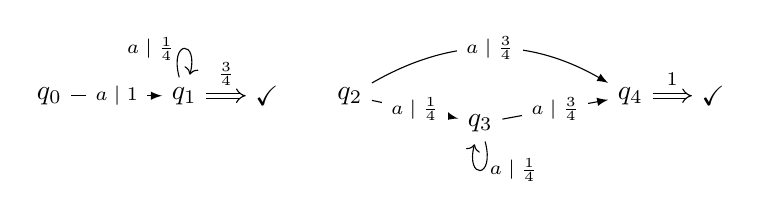
\begin{tikzpicture}[baseline=-3ex]
        \node (0) {$q_0$};
        \node (1) [right= 1.15 cm of 0]{$q_1$};
        \draw (0) edge[-latex] node[ fill=white] {\scriptsize\( {a} \mid {1}\)} (1);
        \draw (1) edge[loop above] node[left] {\scriptsize\( {a} \mid {\frac{1}{4}}\)} (1);
        \node (o1) [right= 0.5 cm of 1]{$\checkmark$};
        \draw (1) edge[-implies, double, double distance=0.5mm] node[above] {\scriptsize\( \frac{3}{4}\)} (o1);
        \node (2) [right= 0.5 cm of o1] {$q_2$};
         \node (2a) [right= 1.25 cm of 2] {};
        \node (3) [below= -.01 cm of 2a] {$q_3$};
        \draw (2) edge[-latex] node[ fill=white] {\scriptsize\( {a} \mid {\frac{1}{4}}\)} (3);
        \draw (3) edge[loop below] node[right] {\scriptsize\( {a} \mid {\frac{1}{4}}\)} (3);
        \node (4) [right= 3 cm of 2] {$q_4$};
        \draw (3) edge[-latex] node[ fill=white] {\scriptsize\( {a} \mid {\frac{3}{4}}\)} (4);
        \draw (2) edge[-latex, bend left] node[ fill=white] {\scriptsize\( {a} \mid {\frac{3}{4}}\)} (4);
        \node (o2) [right= 0.5 cm of 4]{$\checkmark$};
        \draw (4) edge[-implies, double, double distance=0.5mm] node[above] {\scriptsize\( 1\)} (o2);
\end{tikzpicture}
\end{gather*}
%States $q_0$ and $q_2$ despite not being bisimilar (in the sense from~\cite{Larsen:1991:Bisimulation}), 
States $q_0$ and $q_2$ both assign probability $0$ to the empty word $\emptyword$ and each word $a^{n+1}$ is mapped to the probability $\left(\frac{1}{4}\right)^n \cdot \frac{3}{4}$. Later, we show that the languages generated by states $q_0$ and $q_2$ can be specified using expressions $a\seq a^{\left[ \frac{1}{4} \right]}$ and $a \oplus_{\frac{3}{4}} ( a\seq a^{\left[ \frac{1}{4} \right]} \seq a)$ respectively.
\end{example}
In \Cref{c4:sec:operational}, we will associate to each {PRE} $e$ an operational semantics or, more precisely, a state $q_e$ in a {GPTS}. The language semantics $\sem{e}$ of $e$ will then be the language $\langmap( q_e) \colon \alphabet^\ast \to \interval{0}{1}$ generated by $q_e$. Two {PRE} $e$ and $f$ are language equivalent if $\langmap(q_e)=\langmap(q_f)$. One of our main goals is to present a complete inference system to reason about language equivalence. In a nutshell, we want to present a system of (quasi-)equations of the form $e \equiv f$ such that:
\[
e\equiv f \Leftrightarrow \sem {e} = \sem{g} \Leftrightarrow \langmap(e) = \langmap(f)
\]
Such an inference system will have to contain rules to reason about all constructs of {PRE}, including probabilistic choice and loops. We describe next the system, with some intuition for the inclusion of each group of rules. 

\subsection{Axiomatisation of language equivalence of {PRE}}\label{c4:subsec:axiomatisation}
We define ${\equiv} \subseteq \PExp \times \PExp$ to be the least congruence relation closed under the axioms shown on \Cref{c4:fig:axioms}. We will show in \Cref{c4:sec:completeness} that these axioms are complete with respect to language semantics. 
\begin{figure}[h]
\begin{center}	
{
\small
\(
\begin{array}{ll}
&\textbf{Probabilistic choice}\\
(\mathsf{C1})\;\; 
&  e \oplus_p e \equiv e \\
(\mathsf{C2})\;\; 
&  e \oplus_1 f \equiv  e  \\
(\mathsf{C3})\;\; 
&  e \oplus_p f \equiv f \oplus_{1-p} e  \\
(\mathsf{C4})\;\; 
&  (e \oplus_{p} f) \oplus_{q} g \equiv e \oplus_{pq} \left(f \oplus_{\frac{{(1-p)}q}{1-pq}} g\right)  \\\\
&\textbf{Sequential composition}\\
	(\mathsf{1S})\;\; 
&  \one \seq e \equiv e \,, \\
(\mathsf{S})\;\; 
&  e \seq (f \seq g) \equiv (e \seq f) \seq g \,, \\
(\mathsf{S1})\;\; 
&  e \seq \one \equiv e \,, \\
(\mathsf{0S})\;\; 
&  \zero \seq e \equiv \zero \,, \\
(\mathsf{S0})\;\; 
&  e \seq \zero \equiv \zero \,, \\
(\mathsf{D1})\;\; 
&  e \seq (f \oplus_p g) \equiv e \seq f \oplus_p e \seq g  \\
(\mathsf{D2})\;\; 
&  (e \oplus_p f) \seq g \equiv e \seq g \oplus_p f \seq g \\\\

%% recursion
&\textbf{Loops} \\
(\mathsf{Unroll})\;\; &  e^{[p]} \equiv e \seq e^{[p]} \oplus_p \one  \\[1.2ex]
(\mathsf{Tight})\;\; & (e \oplus_p 1)^{[q]}  \equiv e^{\left[\frac{pq}{1-(1-p)q}\right]}  \\[1.2ex]
(\mathsf{Div})\;\; & 1^{[1]}  \equiv 0  \\[1.2ex]
(\mathsf{Unique})\;\; & \inferrule{g \equiv e\seq g \oplus_p f \quad \fcolorbox{red}{white}{$E(e)=0$}}{g \equiv e^{[p]}\seq f} \\\\
%%(\Fix)\;\; & \{ s \equiv_b t[s / X] \}  s \equiv_b \rec{X}{t} \,, \text{ for $X$ guarded in $t$} \,, \\
%% distance
\
\end{array}
\)\\
\textbf{Termination conidition: $E \colon \PExp \to \interval{0}{1}$}\\
\fcolorbox{red}{white}{$
        \begin{array}{l}
            \quad E(\one)=1 \qquad E(\zero)=E(a) = 0 \qquad
            E \left( e \oplus_p f \right)=pE(e) + {(1-p)}E(f)\\[1.4ex]
            E(e\seq f)=E(e)E(f)\qquad
            \quad E\left(e^{[p]}\right)=
                \begin{cases}
                0 &  \text{\scriptsize $E(e)=1 \wedge p=1$} \\ 
                \frac{1-p}{1-pE(e)} & \text{\scriptsize otherwise}
                \end{cases}   
                \end{array}$
     }
}
\end{center}	
\caption{Axioms for language equivalence of PRE. The rules involving the division of probabilities are defined only when the denominator is non-zero. The function $E(-)$ provides a termination side condition to the (\textsf{Unique}) fixpoint axiom.}
\label{c4:fig:axioms}
\end{figure}

%\begin{figure*}
%        \centering
%        \begin{multicols}{2}
%        	 \begin{flushleft}\underline{\bf Probabilistic Choice}  	 \end{flushleft}
%        \begin{alignat*}{4}
%		\textbf{(C1)} & \;\, 
%		& e &{} \equiv e \oplus_p e\\
%				\textbf{(C2)} & \;\, 
%		& e &{} \equiv e \oplus_1 f\\
%		\textbf{(C3)} & \;\, 
%		& e \oplus_p  f &{} \equiv f \oplus_{\overline{p}} e\\
%		\textbf{(C4)} & \;\, 
%		& (e \oplus_{p} f) \oplus_{q} g & {} \equiv e \oplus_{pq} (f \oplus_{\frac{{(1-p)}q}{1-pq}} g)\\
%		\textbf{(D1)} & \;\, 
%		& (e \oplus_{p} f) \seq g & {} \equiv e \seq g \oplus_{p} f \seq g\\[-0.25ex]
%		\textbf{(D2)} & \;\, 
%		& e \seq (f \oplus_{p} g) & {} \equiv e \seq g \oplus_{p} e \seq f\\[-0.25ex]\\\\
%        \end{alignat*}
%          \begin{flushleft}   \underline{\bf Sequencing} \end{flushleft}
%        \begin{alignat*}{4}
%        \textbf{(0S)} & \;\, 
%		& 0 \seq e & {} \equiv 0 & \\[-0.25ex]
%		\textbf{(S0)} & \;\, 
%		& e \seq 0 & {} \equiv 0 & \\[-0.25ex]
%		\textbf{(1S)} & \;\, 
%		& 1 \seq e & {} \equiv e & \\[-0.25ex]
%		\textbf{(S1)} & \;\, 
%		& e \seq 1 & {} \equiv e \\[-0.25ex]
%		\textbf{(S)} & \;\, 
%		& e \seq (f \seq g) & {} \equiv (e \seq f ) \seq g \\[-0.25ex]
%        \end{alignat*}
%        \end{multicols}
%        \vspace{-2cm}
%         \begin{multicols}{2}
%     \begin{flushleft}    \underline{\bf Loops} \end{flushleft}
%        \begin{alignat*}{4}
%       	\textbf{(Unroll)} & \;\, 
%		& e \seq e^{[p]} \oplus_p 1& {} \equiv e^{[p]} \\
%		\textbf{(Tight)} & \;\, 
%		& (e \oplus_p 1)^{[q]} \seq 1 & {} \equiv e^{\left[\frac{pq}{1-\ol{p}q}\right]} \\[-0.25ex]
%		\textbf{(Div)} & \;\, 
%		& 1^{[1]} & {} \equiv 0 \\
%%		 \\ \quad\;\;\textbf{(Unique)} \;\, 
%%		\rlap{$\inferrule{g \equiv e\seq g \oplus_p f \quad \fcolorbox{red}{white}{$E(e)=0$}}{g \equiv e^{[p]}\seq f}$}
%        \end{alignat*}
%          \begin{flushleft}   \underline{\bf (Unique) fixpoint rule} \end{flushleft}
%		$\inferrule{g \equiv e\seq g \oplus_p f \quad \fcolorbox{red}{white}{$E(e)=0$}}{g \equiv e^{[p]}\seq f}$
%\end{multicols}
%        \vspace{-.5cm}
%     \begin{flushleft}    \underline{\bf Termination cond. $E : \PExp \to \interval{0}{1}$} \end{flushleft}
%        \fcolorbox{red}{white}{$
%        \begin{array}{l}
%            \quad E(\one)=1 \qquad E(\zero)=E(a) = 0 \qquad
%            E \left( e \oplus_p f \right)=pE(e) + \ol{p}E(f)\qquad 
%            E(e\seq f)=E(e)E(f)\quad \\[1.4ex]
%            \quad E\left(e^{[p]}\right)=
%                \begin{cases}
%                0 &  \text{\scriptsize $E(e)=1 \wedge p=1$} \\ 
%                \frac{1-p}{1-pE(e)} & \text{\scriptsize otherwise}
%                \end{cases}   
%                \end{array}$
%     }
%     %        \end{tabular}
%      %		\begin{align*}
%%            \textbf{(Unroll)} \quad e^{[p]} &\equiv e \seq e^{[p]}\\
%%            \textbf{(Tight)} \quad (e \oplus_p \one)^{[q]} &\equiv e^{\left[\frac{pq}{1-\ol{p}q}\right]}\\
%%            \one^{[1]} &\equiv \zero &\textbf{(Div)}\\
%%           \omit\rlap{$\inferrule{g \equiv e\seq g \oplus_p f \quad \fcolorbox{red}{white}{$E(e)=0$}}{g \equiv e^{[p]}\seq f}$}&&\textbf{(Unique)}\\
%%        \end{align*}
%        \caption{\label{fig:axioms} For $p \in \interval{0}{1}$, we write $\ol{p}=1-p$. The rules involving the division of probabilities are defined only when the denominator is non-zero. The function $E(-)$ provides a termination side condition to the \textbf{Unique} fixpoint axiom.}
%            \vspace{-.4cm}
%    \end{figure*}
%We will also write ${\equiv_b} \subseteq {\PExp \times \PExp}$ for the least congruence relation containing all the above rules except the two marked with $\heartsuit$. Intuitively, removing these rules axiomatises bisimilarity, which is the finer notion of equivalence. This relation will be used in the intermediate step of the proof of soundness. We will use the following notation for the quotient maps:
%% https://q.uiver.app/?q=WzAsMyxbMSwwLCJ7XFxFeHB9L3tcXGVxdWl2XzB9Il0sWzIsMCwie1xcRXhwfS97XFxlcXVpdn0iXSxbMCwwLCJcXEV4cCJdLFswLDEsIlstXV97XFxlcXVpdn0iLDJdLFsyLDAsIlstXV97XFxlcXVpdl8wfSIsMl0sWzIsMSwiWy1dIiwwLHsiY3VydmUiOi0zfV1d
%\[\begin{tikzcd}
%	\PExp & {{\PExp}/{\equiv_b}} & {{\PExp}/{\equiv}}
%	\arrow["{[-]_{\equiv}}"', from=1-2, to=1-3]
%	\arrow["{[-]_{\equiv_b}}"', from=1-1, to=1-2]
%	\arrow["{[-]}", curve={height=-18pt}, from=1-1, to=1-3]
%\end{tikzcd}\]

The first group of axioms capture properties of the probabilistic choice operator $\oplus_p$ (\textsf{C1-C4}) and its interaction with sequential composition (\textsf{D1-D2}). Intuitively, (\textsf{C1-C4}) are the analogue of the semilattice axioms governing the behaviour of $+$ in regular expressions. These four axioms are reminiscent of the axioms of barycentric algebras~\cite{Stone:1949:Postulates}. (\textsf{D1}) and (\textsf{D2}) are \emph{right and left distributivity} rules of $\oplus$ over $\seq$. The sequencing axioms (\textsf{1S}), (\textsf{S1}), (\textsf{S})  state {PRE} have the structure of a monoid (with neutral element $\one$ with absorbent element $\zero$ -- see axioms (\textsf{0S}), (\textsf{S0}). The loop axioms contain respectively \emph{unrolling}, \emph{tightening}, and \emph{divergency} axioms plus a \emph{unique fixpoint} rule. The (\textsf{Unroll}) axiom associates loops with their intuitive behaviour of choosing, at each step, probabilistically between successful termination and executing the loop body once. (\textsf{Tight}) and (\textsf{Div}) are the probabilistic analogues of the identity $(e + \one)^{*} \equiv e^{*}$ from regular expressions. In the case of {PRE}, we need two axioms: (\textsf{Tight}) states that the probabilistic loop whose body might instantly terminate, causing the next loop iteration to be executed immediately is provably equivalent to a different loop, whose body does not contain immediate termination; (\textsf{Div}) takes care of the edge case of a no-exit loop and identifies it with failure. Finally, the unique fixpoint rule is a re-adaptation of the analogous axiom from Salomaa's axiomatisation and provides a partial converse to the loop unrolling axiom, given the loop body is productive -- i.e. cannot immediately terminate. This productivity property is formally written using the side condition $E(e) = 0$, which can be thought of as the probabilistic analogue of empty word property from Salomaa’s axiomatisation. Consider an expression $a^{\left[\frac{1}{2}\right]} \seq (b \oplus_{\frac{1}{2}} \one)$. The only way it can accept the empty word is to leave the loop with the probability of $\frac{1}{2}$ and then perform $1$, which also can happen with probability $\frac{1}{2}$. In other words, $\llbracket a^{\left[\frac{1}{2}\right]} \seq (b \oplus_{\frac{1}{2}} \one)\rrbracket(\emptyword) = \frac{1}{4}$. A simple calculation allows to verify that $E( a^{\left[\frac{1}{2}\right]} \seq (b \oplus_{\frac{1}{2}} \one)) = \frac{1}{4}$.




\begin{example} We revisit the expressions from \Cref{c4:ex:systems} and show their equivalence via axiomatic reasoning.
\begin{align*}
     a \seq a^{[\frac{1}{4}]} &\equiv a \seq (a^{[\frac{1}{4}]} \seq a \oplus_{\frac{1}{4}} \one) \tag{$\dagger$}\\ 
     &\equiv  (a \seq a^{[\frac{1}{4}]}\seq a) \oplus_{\frac{1}{4}} a \seq \one \tag{\textsf{D2}}\\
     &\equiv (a \seq a^{[\frac{1}{4}]}\seq a) \oplus_{\frac{1}{4}} a \tag{\textsf{S1}}\\
     &\equiv a \oplus_{\frac{3}{4}} (a \seq a^{[\frac{1}{4}]}\seq a)  \tag{\textsf{C3}}
\end{align*}

The $\dagger$ step of the proof above relies on the equivalence $e^{[p]}\seq e \oplus_p \one \equiv e$ derivable from other axioms under the assumption $E(e)=0$ through a following line of reasoning:
\begin{align*}
    e^{[p]} \seq e \oplus_p \one  &\equiv (e \seq e^{[p]} \oplus_p \one)\seq e\oplus_p \one \tag{\textsf{Unroll}}\\
    &\equiv (e \seq e^{[p]}\seq e \oplus_p \one\seq e) \oplus_p \one \tag{\textsf{D1}}\\
    &\equiv (e \seq e^{[p]}\seq e \oplus_p e) \oplus_p \one \tag{\textsf{1S}}\\
        &\equiv (e \seq e^{[p]}\seq e \oplus_p e\seq \one) \oplus_p \one \tag{\textsf{S1}}\\
    &\equiv e \seq (e^{[p]}\seq e \oplus_p \one) \oplus_p \one \tag{\textsf{D2}}
\end{align*}
Since $E(e)=0$,  we then have: 
\(
     e^{[p]} \seq e \oplus_p \one \stackrel{(\textsf{Unique})}\equiv e^{[p]}\seq \one 
     \stackrel{(\textsf{S1})}\equiv e^{[p]} .
\)
\end{example}
\section{Preliminaries}\label{c4:sec:preliminiaries}
In this section, we review the main preliminaries for the technical development outlined in the subsequent sections. 
\label{c4:sec:preliminaries}
\subsection{Locally finitely presentable categories}\label{c4:subsec:lfp}
In this chapter, we will rely on notions associated with the theory of locally finitely presentable categories~\cite{Adamek:1994:Locally}, that allows to generalise the notion of \emph{finiteness} to more structured categories than just $\Set$.

$\D$ is a filtered category, if every finite subcategory $\D_0 \hookrightarrow \D$ has a cocone in $\D$. A filtered colimit is a colimit of the diagram $\D \to \C$, where $\D$ is a filtered category. A directed colimit is a colimit of the diagram $\D \to \C$, where $\D$ is a directed poset. We call a functor \emph{finitary} if it preserves filtered colimits. An object $C$ is \emph{finitely presentable (fp)} if the representable functor $\C(C,-) \colon \C \to \Set$ preserves filtered colimits. Similarly, an object $C$ is \emph{finitely generated (fg)} if the representable functor $\C(C,-) \colon \C \to \Set$ preserves directed colimits of monomorphisms. Importantly, every finitely presentable object is finitely generated, but the converse does not hold in general. 
\begin{definition}
A category $\C$ is \emph{locally finitely presentable (lfp)} if it is cocomplete and there exists a set of finitely presentable objects, such that every object of $\C$ is a filtered colimit of objects from that set.	
\end{definition}
 $\Set$ is the prototypical example of a locally finitely presentable category, where finitely presentable objects are precisely finite sets.

\subsection{Monads and their algebras}\label{c4:subsec:monads}
A monad (over the category $\Set$) is a triple $\monadT = (T, \mu, \eta)$ consisting of a functor $T \colon \Set \to \Set$ and two natural transformations: a unit $\eta \colon \Id \Rightarrow T$ and multiplication $\mu \colon T^2 \Rightarrow T$ satisfying $\mu \circ \eta_T = \id_T=  \mu \circ T\eta$ and $\mu \circ \mu_T = \mu \circ T \mu$
A $\monadT$-algebra (also called an Eilenberg-Moore algebra) for a monad $T$ is a pair $(X, h)$ consisting of a set $X \in \Obj(\C)$, called carrier, and a function $h \colon T X \to X$ such that $h \circ \mu_X = h \circ Th$ and $h \circ \eta_X = \id_X$. A $\monadT$-algebra homomorphism between two $T$-algebras $(X,h)$ and $(Y,k)$ is a function 	$f \colon X \to Y$ satisfying $k \circ Tf = f \circ h$.

$\monadT$-algebras and $\monadT$-homomorphisms form a category $\Set^\monadT$. There is a canonical forgetful functor $\forget \colon \Set^\monadT \to \Set$ that takes each $\monadT$-algebra to its carrier. This functor has a left adjoint $X \mapsto (TX, \mu_X \colon T^2 X \to T)$, mapping each set to its free $\monadT$-algebra. If $X$ is finite, then we call $(TX, \mu_X)$ free finitely generated.

Given a function $f \colon X \to Y$, where $Y$ is a carrier of a $\monadT$-algebra $(Y, h)$, there is a unique homomorphism $f^\sharp \colon (TX, \mu_X) \to (Y,h)$ satisfying $f^\sharp \circ \eta_X = f$ that is explicitly given by $f^\sharp = h \circ Tf$.

\subsection{Generalised determinisation}\label{sec:c4:generalised_determinisation}
Language acceptance of nondeterministic automata (NDA) can be captured via determinisation. {NDA} can be viewed as coalgebras for the functor $N = 2 \times {\powf}^\alphabet$, where $\powf$ is the finite powerset monad. Determinisation converts a {NDA} $(X, \beta \colon X \to 2 \times {\powf X}^\alphabet)$ into a deterministic automaton $\left({\powf X}, \beta^{\sharp} \colon {\powf X} \to 2 \times {(\powf X)}^\alphabet \right)$, where for $A \subseteq X$, we define $\beta^{\sharp}(A) = \bigcup_{x \in \alphabet} \beta(a)$. Additionally, $\beta^\sharp$ satisfies $\beta^\sharp(\{x\}) = \beta(x)$ for all $x \in X$. A language of the state $x \in X$ of {NDA}, is given by the language accepted by the state $\{x\}$ in the determinised automaton $({\powf X}, \beta^\sharp)$. 


This construction can be generalised~\cite{Silva:2010:Generalizing} to $HT$-coalgebras, where $T \colon \Set \to \Set$ is an underlying functor of finitary monad $\monadT$ and $H \colon \Set \to \Set$ an endofunctor that admits a final coalgebra that can be lifted to the functor $\overline{H} \colon \Set^\monadT \to \Set^\monadT$. Liftings of functors $H \colon \Set \to \Set$ to $\overline{H} \colon \Set^\monadT \to \Set^\monadT$, are in one-to-one correspondence with distributive laws of the monad $\mathsf{T}$ over the functor $H$~\cite{Jacobs:2015:Trace}, which are natural transformations $\rho \colon TH \Rightarrow HT$ satisfying
$H\eta_X = \rho_X \circ \eta_{HX}$ and $H \mu_X \circ \rho_{TX} \circ T\rho_X = \rho_X \circ \mu_{HX}$. In particular, given a $\monadT$-algebra $(X, k \colon TX \to X)$, we can equip $HX$, with a $\monadT$-algebra structure, given by the following composition of maps:
% https://q.uiver.app/#q=WzAsMyxbMCwwLCJUSFgiXSxbMiwwLCJIVFgiXSxbNCwwLCJIWCJdLFswLDEsIlxccmhvX1giXSxbMSwyLCJIdCJdXQ==
\[\begin{tikzcd}
	THX && HTX && HX
	\arrow["{\rho_X}", from=1-1, to=1-3]
	\arrow["Ht", from=1-3, to=1-5]
\end{tikzcd}\]


Generalised determinisation turns $HT$-coalgebras $(X, \beta \colon X \to HT X)$ into $H$-coalgebras $(T X , \beta^\sharp \colon T X \to H T X)$, where $\beta^\sharp$ is the unique extension arising from the free-forgetful adjunction between $\Set$ and $\Set^\monadT$. The language of a state $x \in X$ is given by $\beh{\beta^\sharp} \circ \eta_X \colon X \to \nu H$, where $\eta$ is the unit of the monad $\monadT$. Since $\beta^\sharp \colon TX \to HTX$ can be seen as a $\monadT$-algebra homomorphism $(TX, \mu_X) \to \overline{H}(TX, \mu_X)$, each determinisation $(TX, \beta^{\sharp})$ can be viewed as an $\overline{H}$-coalgebra $((TX, \mu_X), \beta^{\sharp})$. The carrier of the final $H$-coalgebra can be canonically equipped with $\monadT$-algebra structure, yielding the final $\overline{H}$-coalgebra. In such a case, the unique final homomorphism from any determinisation (viewed as an $H$-coalgebra) is precisely an underlying function of the final $\overline{H}$-coalgebra homomorphism. 

\subsection{Subdistribution monad}\label{c4:subsec:subdistribution}
 A function $\nu \colon X \to \interval{0}{1}$ is called a subprobability distribution or subdistribution, if it satisfies $\sum_{x \in X} \nu(x) \leq 1$. A subdistribution $\nu$ is \emph{finitely supported}  if the set $\supp(\nu) = \{x \in X \mid \nu(x) > 0\}$ is finite. We use $\distf {X}$ to denote the set of finitely supported subprobability distributions on $X$. The weight of a subdistribution $\nu \colon X \to \interval{0}{1}$ is a total probability of its support:
$$|\nu| = \sum_{x \in X} \nu(x)$$
Given $\nu\in\distf X$ and $Y \subseteq X$, we will write $\nu[Y] = \sum_{x \in Y} \nu(x)$. This sum is well-defined as only finitely many summands have non-zero probability. 
 
  
 Given $x \in X$, its \emph{Dirac} is a subdistribution $\delta_x$ which is given by $\delta_x(y)=1$ only if $x=y$, and $0$ otherwise. We will moreover write $\emptydist \in \distf X$ for a subdistribution with an empty support. It is defined as $\emptydist(x)=0$ for all $x \in X$. When $\nu_1, \nu_2 \colon X \to \interval{0}{1}$ are subprobability distributions and $p \in \interval{0}{1}$, we write $p\nu_1 + (1-p)\nu_2$ for the convex combination of $\nu_1$ and $\nu_2$, which is the probability distribution given by $$(p \nu_1 + (1-p) \nu_2)(x) = p\nu_1(x) + (1-p)\nu_2(x)$$
 for all $x \in X$. Note that this operation preserves finite support. 
 
  $\distf$ is in fact a functor on the category $\Set$, which maps each set $X$ to $\distf X$ and maps each arrow $f \colon X \to Y$ to the function $\distf \funF \colon \distf X \to \distf Y$ given by $$\distf \funF (\nu)(x) = \sum_{y \in f^{-1}(x)} \nu(y)$$
   Moreover, $\distf$ also  carries a monad structure with unit  $\eta_X(x) = \delta_x$ and multiplication $\mu_X(\Phi)(x) = \sum_{\varphi \in \distf X }\Phi(\varphi)\varphi(x)$ for $\Phi \in \distf^2 X$. Using the free-forgetful adjunction between $\Set$ and category of $\distf$-algebras, given $f \colon X \to \distf Y$, there exists a unique map $f^\sharp \colon \distf X \to \distf Y$ satisfying $f = f^\sharp \circ \delta$ called the \emph{convex extension of $f$}, and explicitly given by $f^\sharp(\nu)(y) = \sum_{x \in X} \nu(x) f(x)(y)$.
   
\subsection{Positive convex algebras}\label{c4:subsec:positive}
By $\sigpca$ we denote a signature given by
$$\sigpca = \left\{\bigboxplus_{i \in I} p_i \cdot (-)_i \mid I \text{ finite}, \forall i \in I \ldotp p_i \in \interval{0}{1}, \sum_{i \in I} p_i \leq 1\right\} $$
A positive convex algebra is a an algebra for the signature $\sigpca$, that is a pair $\A = \left(X, \sigpca^\A\right)$, where $X$ is the carrier set and $\sigpca^\A$ is a set of interpretation functions $\bigboxplus_{i \in I} p_i \cdot (-)_i \colon X^{|I|} \to X$ satisfying the axioms:
\begin{enumerate}
    \item (Projection) \(\bigboxplus_{i \in I} p_i \cdot x_i = x_j\) if \(p_j=1\)
    \item (Barycenter) \(\bigboxplus_{i \in I} p_i \cdot \left(\bigboxplus_{j \in J}{q_{i,j}} \cdot {x_j}\right) = \bigboxplus_{j \in J} \left(\sum_{i \in I} p_i q_{i,j} \right) \cdot x_j\)
\end{enumerate}
In terms of notation, we denote the unary sum by $p_0 \cdot x_0$. Throughout this chapter we will we abuse the notation by writing $$\left(\bigboxplus_{i \in I} p_i \cdot e_i\right) \boxplus \left(\bigboxplus_{i \in J} q_j \cdot f_j\right)$$ for a single sum $\bigboxplus_{k \in I + J} r_k \cdot g_k$, where $r_k = p_k$ and $g_k = e_k$ for $k \in I$ and similarly $r_k = q_k$ and $g_k = f_k$ for $k \in J$. Note that this is well-defined only if $\sum_{i \in I} p_i + \sum_{j \in J} r_j \leq 1$.

The signature of positive convex algebras can be alternatively presented as a family of binary operations, in the following way:

\begin{proposition}[{\cite[Proposition~7]{Bonchi:2017:Power}}]\label{c4:prop:binary}
    If  $X$ is a set equipped with a binary operation $\boxplus_{p} : X \times X \to X$ for each $p \in \interval{0}{1}$ and a constant $0_\boxplus \in X$ satisfying for all $x,y,z \in X$ (when defined) the following:
    \begin{gather*}
        x \boxplus_{p} x = x \qquad x \boxplus_{1} y = x \qquad x \boxplus_{p} y = y \boxplus_{1-{p}} x \\ (x \boxplus_{p} y) \boxplus_{q} z = x \boxplus_{pq} \left(y \boxplus_{\frac{(1-p)q}{1-pq}} z\right)
    \end{gather*}
    then $X$ carries the structure of a positive convex algebra. The interpretation of $\boxplus_{i \in I} p_i \cdot (-)_{i}$ is defined inductively by the following
    $$\bigboxplus_{i \in I} p_i \cdot x_i = \begin{cases}
        0_\boxplus & \text{if } I = \emptyset \\
        x_0 & \text{if } p_0 = 1\\
        x_n \boxplus_{p_k} \left(\bigboxplus_{i \in I \setminus \{k\}} \frac{p_i}{1-{p_k}}\cdot x_i  \right) &\text{otherwise, for some } k \in I
    \end{cases} $$
\end{proposition}

Below we state several properties of positive convex algebras, that we will use throughout this chapter.
\begin{proposition}\label{c4:prop:properties_of_positive_convex_algebras}
    Let $I$ be a finite indexed set, and let $\{p_i\}_{i \in I}$ and $\{x_i\}_{i \in I}$ be indexed collections of elements of $\interval{0}{1}$ and $X$ respectively. Then, in any positive convex algebra, the following statements hold:
    \begin{enumerate}
        \item
        $${\bigboxplus_{i \in I} p_i \cdot x_i} = {\bigboxplus_{x \in \bigcup_{i \in I} \{x_i\}} \left(\sum_{x_i = x} p_i\right)\cdot x}$$
        \item Let ${=_R} \subseteq {X \times X}$ be a congruence relation, with $[-]_R \colon X \to X/{=_R}$ being its canonical quotient map. Then, 
        $${\bigboxplus_{i \in I} p_i \cdot x_i} =_R {\bigboxplus_{[x]_R \in \bigcup_{i \in I} \left\{[x_i]_R\right\}} \left(\sum_{x_i =_R x} p_i\right)\cdot x}$$
        \item All terms $\bigboxplus_{i \in I } 0 \cdot x_i $ coincide and are all provably equivalent to the empty convex sum.
        \item If $J \subseteq I$ and $\{i \in I \mid p_i \neq 0\} \subseteq J$, then 
        $$
        \bigboxplus_{i \in I} p_i \cdot x_i = \bigboxplus_{j \in J} p_j \cdot x_j
        $$
        \item Let $\sigma \colon I \to I$ be a permutation of the index set $I$. Then, we have that
        $$
        	\bigboxplus_{i \in I} p_i \cdot x_i = \bigboxplus_{i \in I} p_{\sigma(i)} \cdot x_{\sigma(i)}
        $$
    \end{enumerate}
\end{proposition}
\begin{proof}
    We write $[\Phi]$ to denote Iverson bracket, which is defined to be $1$ if $\Phi$ is true and $0$ otherwise.
    
    For \circlednum{1} we have that
    \begin{align*}
        \bigboxplus_{i \in I} p_i \cdot x_i &= \bigboxplus_{i \in I} p_i \cdot \left( \bigboxplus_{x \in \cup_{i \in I} \{x_i\}} [x_i = x] \cdot  x \right) &\tag{Projection axiom}\\
        &= \bigboxplus_{x \in \cup_{i \in I} \{x_i\}} \left( \sum_{i \in I} p_i[x_i = x] \right) \cdot x \tag{Barycenter axiom} \\
        &=  \bigboxplus_{x \in \cup_{i \in I} \{x_i\} } \left(\sum_{x_i = x} p_i\right) \cdot x
    \end{align*}
    \circlednum{2} can be shown by picking a representative for each equivalence class and then using \circlednum{1}. For \circlednum{3}, by \cite[Lemma~3.4]{Sokolova:2015:Congruences} we know that all terms $\bigboxplus_{i \in I} 0 \cdot x_i$ coincide. To see that they are provably equivalent to the empty convex sum, observe that
    \begin{align*}
        \bigboxplus_{i \in I} 0 \cdot x_i &= \bigboxplus_{i \in I} 0 \cdot \left(\bigboxplus_{j \in \emptyset} p_j \cdot y_j\right)\tag{\cite[Lemma~3.4]{Sokolova:2015:Congruences}}\\
        &= \bigboxplus_{j \in \emptyset} 0 \cdot y_j \tag{Barycenter axiom}\\
    \end{align*}
    Finally, \circlednum{4} follows from \cite[Lemma~3.4]{Sokolova:2015:Congruences}, while \circlednum{5} was proved in \cite[Proposition~3.1]{Doberkat:2008:Erratum}.
\end{proof}
\begin{lemma}\label{c4:lem:flattening_convex_sums}
    Let $I, J$ be finite index sets, $\left\{p_i\right\}_{i \in I}$, $\{q_{i,j}\}_{(i,j) \in I\times J}$ and $\{x_{i,j}\}_{(i,j) \in I \times J}$ indexed collections such that for all $i \in I$ and $j \in J$, $p_i, q_{i,j} \in \interval{0}{1}$ and $x_{i,j} \in X$. If $X$ carries $\pca$ structure, then:
    $$\bigboxplus_{i \in I} p_i \cdot \left(\bigboxplus_{j \in J} q_{i,j} \cdot x_{i,j}\right) = \bigboxplus_{(i,j) \in I \times J} p_iq_{i,j} \cdot x_{i,j}$$
\end{lemma}
\begin{proof}
    \begin{align*}
        \bigboxplus_{i \in I} p_i \cdot \left(\bigboxplus_{j \in J} q_{i,j} \cdot x_{i,j}\right) &= \bigboxplus_{i \in I} p_i \cdot \left(\bigboxplus_{(k,j) \in \{i\} \times J} q_{k,j} \cdot x_{k,j}\right) \\
        &= \bigboxplus_{i \in I} p_i \cdot \left(\bigboxplus_{(k,j) \in I \times J} [k = i]q_{k,j} \cdot x_{k,j}\right) \tag{\Cref{c4:prop:properties_of_positive_convex_algebras}} \\
        &= \bigboxplus_{(k,j) \in I \times J} \left(\sum_{i \in I} p_i [k=i]q_{k,j} \right) \cdot x_{k,j} \tag{Barycenter axiom} \\
        &= \bigboxplus_{(k,j) \in I \times J} p_k q_{k,j}  \cdot x_{k,j} \\
        &= \bigboxplus_{(i,j) \in I \times J} p_i q_{i,j}  \cdot x_{i,j} \tag{Renaming indices}\\
    \end{align*}
\end{proof}
\begin{lemma}\label{c4:lem:grouping_probabilities}
    Let $I$ be a finite index set, $\{p_i\}_{i \in I}$ and $\{q_i\}_{i \in I}$ indexed collections such that $p_i,q_i \in \interval{0}{1}$ for all $i \in I$, $\sum_{i \in I} p_i + \sum_{i \in I} q_i \leq 1$ and let $\{x_i\}_{i \in I}$ and $\{y_i\}_{i \in I}$ indexed collection such that $x_i, y_i \in X$ for all $i \in I$. If $X$ carries $\pca$ structure, then:
    $$
    \left(\bigboxplus_{i \in I} p_i \cdot x_i\right) \boxplus\left(\bigboxplus_{i \in I} q_i \cdot y_i\right) = \bigboxplus_{i \in I} (p_i + q_i) \cdot \left(\frac{p_i}{p_i + q_i} \cdot x_i \boxplus \frac{q_i}{p_i + q_i} \cdot y_i \right)
    $$
\end{lemma}
\begin{proof}
    Let $J = \{0,1\}$. Define indexed collections $\{r_{i,j}\}_{(i,j) \in I \times J}$ and $\{z_{i,j}\}_{(i,j) \in I \times J}$, such that $r_{i,0} = \frac{p_i}{p_i + q_i}$ and $z_{i,0} = x_i$ and $r_{i,1} = \frac{q_i}{p_i + q_i}$ and $z_{i,1} = x_i$.
    We have the following:
    \begin{align*}
        \bigboxplus_{i \in I} (p_i + q_i) \cdot \left(\frac{p_i}{p_i + q_i} \cdot x_i \boxplus \frac{q_i}{p_i + q_i} \cdot y_i\right) &= \bigboxplus_{i \in I} (p_i + q_i) \cdot \left(\bigboxplus_{j \in J} r_{i,j} \cdot z_{i,j} \right) \\
        &= \bigboxplus_{(i,j) \in I \times J} (p_i + q_i)r_{i_j} \cdot z_{i,j} \tag{\Cref{c4:lem:flattening_convex_sums}} \\
        &= \left(\bigboxplus_{i \in I} p_i \cdot x_{i}\right) \boxplus \left(\bigboxplus_{i \in I} q_i \cdot y_i\right)
    \end{align*}
\end{proof}
Speaking more abstractly, positive convex algebras and their homomorphisms (in the sense of homomorphisms of algebras for the signature from universal algebra) form a category, that we will call $\pca$. This category can be seen as a concrete presentation of an Eilenberg-Moore algebra for the subdistribution monad.

\begin{theorem}\label{c4:thm:correspondence}
	There is an isomorphism of categories between $\pca$ and $\Set^{\distf}$. Given a set $X$ equipped with a positive convex algebra structure, we can define a map $h \colon \distf X \to X$, given by 
	$$
		h(\nu) = \bigboxplus_{x \in \supp(\nu)} \nu(x) \cdot x
	$$
	for all $\nu \in \distf X$, making $(X, h)$ into an algebra for the monad $\distf$. Equivalently, given a $\distf$-algebra $(X, h)$, one can define 
	$$
		\bigboxplus_{i \in I} p_i \cdot x_i = h \left(\sum_{i \in I} p_i \cdot \delta_{x_i}\right)
	$$
	for all finite $I$ and indexed collections $\{p_i\}_{i \in I}$, $\{x_i\}_{i \in I}$, such that $\sum_{i \in I} p_i \leq 1$ and for all $i \in I$, $x_i \in X$. This equips the set $X$ with a positive convex algebra structure.  
	\end{theorem}
	\begin{proof}
		See \cite[Theorem~4]{Jacobs:2010:Convexity} or \cite[Proposition~5.3]{Doberkat:2008:Erratum}.
	\end{proof}
	Moreover, $\pca$ as a category enjoys the following property: 
	\begin{theorem}[{\cite{Sokolova:2015:Congruences}}]\label{c4:thm:fp_fg}
		In $\pca$ finitely presented and finitely generated objects coincide.
	\end{theorem}
	\subsection{Rational fixpoint}\label{c4:subsec:rational}
	The completeness claim presented in this chapter will rely on the universal property of the rational fixpoint~\cite{Adamek:2006:Iterative,Milius:2010:Sound}, which provides a convenient notion of a domain representing \emph{finite} behaviours of structured transition systems, by relying on the theory of locally finitely presentable categories.
		
	Let $\funB \colon \C \to \C$ be a finitary functor. We will write $\coaf{\funB}$ for the subcategory of $\coa{\funB}$ consisting only of $\funB$-coalgebras with finitely presentable carrier. The \emph{rational fixpoint} is defined as $$(\varrho \funB,r) = \colim(\coaf{\funB} \hookrightarrow \coa{\funB})$$ In other words, $(\varrho \funB,r)$ is colimit of the inclusion functor from the subcategory of coalgebras with finitely presentable carriers. We call it a fixpoint, as the map $r \colon \varrho \funB \to \funB (\varrho \funB) $ is an isomorphism~\cite{Adamek:2006:Iterative}. 
% The rational fixpoint can be both viewed as a final locally finitely presentable $F$-coalgebra and an initial iterative $F$-algebra~\cite{Adamek:2006:Iterative}. 

Under some restrictions on underlying category and the type functor of coalgebras, we have the following result:
\begin{theorem}[{{\cite[Corollary~3.10, Theorem~3.12]{Milius:2020:New}}}]\label{c4:thm:fully_abstract}
	If finitely presentable and finitely generated objects coincide in $\C$ and $\funB \colon \C \to \C$ is a finitary endofunctor preserving non-empty monomorphisms, then rational fixpoint is fully abstract, that is, $(\varrho B, r)$ is a subcoalgebra of the final coalgebra $(\funB, t)$.
\end{theorem}
The requirement of preserving non-empty monomorphisms is quite weak and is satisfied by any lifting of a $\Set$ endofunctor to the category of Eilenberg-Moore algebras.
\begin{lemma}\label{c4:lem:nonempty_monos}
	Let $H \colon \Set \to \Set$ be an endofunctor and let $\monadT$ be a finitary monad on $\Set$. Then, the lifting $\overline{H} \colon \Set^\monadT \to \Set^\monadT$ preserves non-empty monomorphisms. 
\end{lemma}
\begin{proof}
	Follows from \cite[Corollary~3.16]{Gumm:2000:Elements} and \cite[Lemma~2.4]{Milius:2020:New}.
\end{proof}
\section{Operational semantics}\label{c4:sec:operational}
In this section, we begin by describing a coalgebraic approach to modelling the probabilistic language semantics of GPTS. Building on this, we introduce an operational semantics for PRE, drawing inspiration from Antimirov’s partial derivatives for NFAs~\cite{Antimirov:1996:Partial}.
\subsection{Language semantics of GPTS}\label{c4:subsec:language_semantics}
Let $\funF \colon \Set \to \Set$ be an endofunctor given by $\funF = \{\checkmark\} + \alphabet \times (-)$. GPTS are precisely $\distf \funF$-coalgebras, that is pairs $(X, \beta)$, where $X$ is a set of states and $\beta \colon X \to \distf (\{\checkmark\} + \alphabet \times X)$ is a transition structure. Because of this, we will interchangeably use terms "$\distf \funF$-coalgebra" and "GPTS".

The functor $\distf \funF$ admits a final coalgebra, but unfortunately it is not carried by the set of probabilistic languages, that is $\interval{0}{1}^{\alphabet^{\ast}}$, because the canonical semantics of $\distf \funF$-coalgebras happens to correspond to the more restrictive notion of probabilistic bisimilarity (also known as Larsen-Skou bisimilarity~\cite{Larsen:1991:Bisimulation}). Probabilistic bisimilarity is a branching-time notion of equivalence, requiring observable behaviour of compared states to be equivalent at every step, while probabilistic language equivalence is a more liberal notion comparing sequences of observable behaviour. In general, if two states are bisimilar, then they are language equivalent, but the converse does not hold.
\begin{example}\label{c4:ex:bisimilarity}
 Consider the following {GPTS}:
 \begin{gather*}
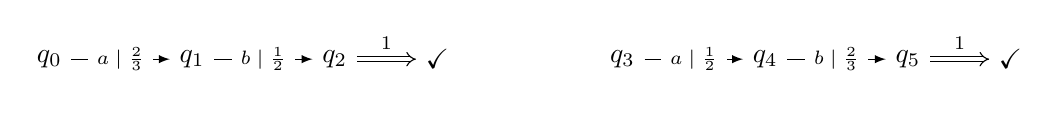
\begin{tikzpicture}[baseline=-3ex]
        \node (0) {$q_0$};
        \node (1) [right= 1.25 cm of 0]{$q_1$};
        \node (2) [right= 1.25 cm of 1]{$q_2$};
        \node (o1) [right= 0.75 cm of 2]{$\checkmark$};
        \node (3) [right = 1.8 cm of o1]{$q_3$};
        \node (4) [right= 1.25 cm of 3]{$q_4$};
        \node (5) [right= 1.25 cm of 4]{$q_5$};
        \node (o2) [right= 0.75 cm of 5]{$\checkmark$};
        \draw (0) edge[-latex] node[ fill=white] {\scriptsize\( {a} \mid {\frac{2}{3}}\)} (1);
		\draw (1) edge[-latex] node[ fill=white] {\scriptsize\( {b} \mid {\frac{1}{2}}\)} (2);
		\draw (2) edge[-implies, double, double distance=0.5mm] node[above] {\scriptsize\( 1\)} (o1);
		\draw (3) edge[-latex] node[ fill=white] {\scriptsize\( {a} \mid {\frac{1}{2}}\)} (4);
		\draw (4) edge[-latex] node[ fill=white] {\scriptsize\( {b} \mid {\frac{2}{3}}\)} (5);
		\draw (5) edge[-implies, double, double distance=0.5mm] node[above] {\scriptsize\( 1\)} (o2);
\end{tikzpicture}
\end{gather*}
States $q_0$ and $q_3$ are language equivalent because they both accept the string $ab$ with the probability $\frac{1}{3}$, but are not bisimilar, because the state $q_0$ can make $a$ transition with the probability $\frac{2}{3}$, while $q_3$ can perform an $a$ transition with probability $\frac{1}{2}$.
\end{example}
A similar situation happens when looking at nondeterministic automata through the lenses of universal coalgebra, where again the canonical notion of equivalence is the one of bisimilarity. A known remedy is the powerset construction from classic automata theory, which converts a nondeterministic automaton to a deterministic automaton, whose states are sets of states of the original nondeterministic automaton we have started from. In such a case, the nondeterministic branching structure is factored into the state space of the determinised automaton. The language of an arbitrary state of the nondeterministic automaton corresponds to the language of the singleton set containing that state in the determinised automaton.

Generalised determinisation extends the above idea to $HT$-coalgebras, where $T \colon \Set \to \Set$ is an underlying functor of a finitary monad $\monadT$ and $H \colon \Set \to \Set$ is a functor that can be lifted to category $\Set^\monadT$ of $\monadT$-algebras. Generalised determinisation provides a uniform treatment of language semantics of variety of transition systems, where the final $H$-coalgebra provides a notion of language. Unfortunately, $\distf \funF$-coalgebras do not fit immediately to this picture.  Luckily, each such $\distf \funF$-coalgebra can be seen as a special case of a more general kind of transition system, known as reactive probabilistic transition systems~({RPTS})~\cite{Glabbeek:1995:Reactive} or Rabin probabilistic automata~\cite{Rabin:1963:Probabilistic}. 



{RPTS} can be intuitively viewed as a probabilistic counterpart of nondeterministic automata and they can be determinised to obtain probabilistic language semantics. In an {RPTS}, each state $x$ is mapped to a pair $\langle o_x,n_x \rangle$, where $o \in \interval{0}{1}$ is the acceptance probability of state $x$ and $n_x\colon \alphabet \to \distf(X)$ is the next-state function, which takes a letter $a \in \alphabet$ and returns the subprobability distribution over successor states. Formally speaking, let $\funG \colon \Set \to \Set$ be an endofunctor $\funG = \interval{0}{1} \times (-)^\alphabet$. RPTS are precisely $\funG\distf$-coalgebras, that is pairs $(X, \beta)$, where $X$ is a set of states and $\beta \colon X \to \interval{0}{1} \times \distf (X)^\alphabet$ is a transition function. Following the convention outlined before, we will use terms "$G\distf$-coalgebras" and "RPTS" interchangeably.

$\funG \distf$-coalgebras fit into framework of generalised determinisation~\cite{Silva:2011:Sound}. In particular, there exists a distributive law $\rho \colon \distf \funG \Rightarrow \funG \distf$ of the monad $\distf$ over the functor $\funG$ that allows to lift $\funG \colon \Set \to \Set$ to $\overline{\funG} \colon \pca \to \pca$. Speaking in concrete terms, if the set $X$ is equipped with a convex sum operation $\bigboxplus_{i \in I} p_i \cdot (-)$, then so is $\interval{0}{1} \times X^\alphabet$. Let $\{\langle o_i , t_i\rangle\}_{i \in I}$ be an indexed collection of elements of $\interval{0}{1} \times X^\alphabet$. Then, we can define
\begin{equation}\label{c4:eqn:pca_on_G}
	\bigboxplus_{i \in I} p_i \cdot \langle o_i, t_i \rangle = \left\langle \sum_{i \in I} p_i\cdot o_i, \lambda a\ldotp \bigboxplus_{i \in I} p_i \cdot t_i(a) \right\rangle
\end{equation}
The final coalgebra for the functor $\funG$ is precisely carried by the set $\interval{0}{1}$ of probabilistic languages.

In order to talk about language semantics of $\distf \funF$-coalgebras, we first provide an informal intuition that each $\distf \funF$-coalgebra can be seen as a special case of a $\funG \distf$-coalgebra.
\begin{example}\label{ex:converting}
Fragment of a {GPTS} (on the left) and of the corresponding RPTS (on the right).
 \begin{gather*}
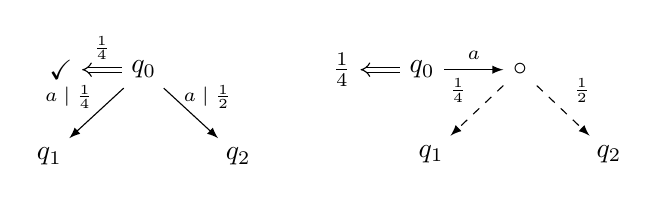
\begin{tikzpicture}[baseline=-3ex]
        \node (o1) {$\checkmark$};
        \node (0) [right= 0.5 cm of o1]{$q_0$};
        \draw (0) edge[-implies, double, double distance=0.5mm] node[above] {\scriptsize\(\frac{1}{4}\)} (o1);
        \node (1) [below left= .9 cm of 0]{$q_1$};
        \node (2) [below right= .9 cm of 0]{$q_2$};
        \draw (0) edge[-latex] node[above, pos=0.6] {\scriptsize\( {a} \mid {\frac{1}{4}}\qquad  \)} (1);
        \draw (0) edge[-latex] node[above, pos=0.6] {\scriptsize\(\quad {a} \mid {\frac{1}{2}}\)} (2);
        \node (o2) [right= 2cm of 0]{$\frac{1}{4}$};
        \node (3) [right= 0.5 cm of o2]{$q_0$};
        \draw (3) edge[-implies, double, double distance=0.5mm] (o2);
        \node (4) [right= 0.75 cm of 3]{$\circ$};
        \draw (3) edge[-latex] node[above] {\scriptsize\( {a}\)} (4);
        \node (5) [below left= 0.9 cm of 4]{$q_1$};
        \node (6) [below right= 0.9 cm of 4]{$q_2$};
        \draw (4) edge[-latex, dashed] node[left, pos = 0.1] {\scriptsize\( {\frac{1}{4}}\quad\)} (5);
        \draw (4) edge[-latex, dashed] node[right, pos = 0.1] {\scriptsize\(\quad {\frac{1}{2}}\)} (6);
%        \node (2) [right= 1.25 cm of 1]{$q_2$};
%        \node (o1) [right= 0.75 cm of 2]{$\checkmark$};
%        \node (3) [below = 0.6 cm of 0]{$q_3$};
%        \node (4) [right= 1.25 cm of 3]{$q_4$};
%        \node (5) [right= 1.25 cm of 4]{$q_5$};
%        \node (o2) [right= 0.75 cm of 5]{$\checkmark$};
%        \draw (0) edge[-latex] node[ fill=white] {\scriptsize\( {a} \mid {\frac{2}{3}}\)} (1);
%		\draw (1) edge[-latex] node[ fill=white] {\scriptsize\( {b} \mid {\frac{1}{2}}\)} (2);
%		\draw (2) edge[-implies, double, double distance=0.5mm] node[above] {\scriptsize\( 1\)} (o1);
%		\draw (3) edge[-latex] node[ fill=white] {\scriptsize\( {a} \mid {\frac{1}{2}}\)} (4);
%		\draw (4) edge[-latex] node[ fill=white] {\scriptsize\( {b} \mid {\frac{2}{3}}\)} (5);
\end{tikzpicture}
\end{gather*}
In the corresponding {RPTS} state $q_0$ accepts with probability $\frac{1}{4}$ and given input $a$ it transitions to subprobability distribution that has $\frac{1}{4}$ probability of going to to $q_1$ and $\frac{1}{2}$ probability of going to $q_2$. \end{example}

We can make the above intuition formal. Let $X$ be a set, and let $\zeta \in \distf \funF X$. Define a function $\gamma_X \colon \distf \funF X \to \funG \distf X$, given by
$$
\gamma_X(\zeta) = \langle \zeta(\checkmark), \lambda a \ldotp \lambda x\ldotp \zeta(a,x)\rangle
$$
Such functions define components of the natural transformation.
\begin{proposition}{\cite{Silva:2011:Sound}}\label{c4:prop:natural}
	$\gamma \colon \distf \funF \Rightarrow \funG \distf$ is a natural transformation with injective components. 
\end{proposition}
We now have all ingredients to specify language semantics of $\distf \funF$-coalgebras. Given a $\distf \funF$-coalgebra  $(X, \beta)$, one can use the natural transformation $\gamma$ and obtain $\funG \distf$-coalgebra $(X, \gamma_X \circ \beta)$. Since $\funG$ can be lifted to $\pca$, we can obtain $\funG$-coalgebra $\left(\distf X, (\gamma_X \circ \beta)^\sharp\right)$. Note that this coalgebra carries an additional algebra structure and its transition map is a $\pca$ homomorphism, thus making $\left( (\distf X, \mu_X), (\gamma_X \circ \beta)^\sharp \right)$ into a $\overline{\funG}$-coalgebra. The resulting language semantics of $(X, \beta)$ are given by the map $\langmap_{(X, \beta)} \colon X \to \interval{0}{1}^\alphabet$ explicitly given by $$\langmap_{(X, \beta)} = \beh{(\gamma_X \circ \beta)^\sharp} \circ \eta_X$$ where $\eta \colon X \to \distf X$ is a unit of the monad $\distf$ taking each state $x \in X$ to its Dirac $\delta_x \in \distf X$.

This can be summarised by the following commutative diagram:
% https://q.uiver.app/#q=WzAsNixbMCwwLCJYIl0sWzAsMSwiXFxkaXN0ZiBcXGZ1bkYgWCJdLFsxLDAsIlxcZGlzdGYgWCJdLFswLDIsIlxcZnVuRyBcXGRpc3RmIFgiXSxbMywwLCJcXGludGVydmFsezB9ezF9XlxcYWxwaGFiZXQiXSxbMywyLCJcXGZ1bkcgXFxsZWZ0KFxcaW50ZXJ2YWx7MH17MX1ee1xcYWxwaGFiZXR9XFxyZ2l0aCkiXSxbMCwxLCJcXGJldGEiXSxbMSwzLCJcXGdhbW1hX1giXSxbMCwyLCJcXGV0YV9YIl0sWzIsMywiKFxcZ2FtbWFfWCBcXGNpcmMgXFxiZXRhKV5cXHNoYXJwIiwwLHsic3R5bGUiOnsiYm9keSI6eyJuYW1lIjoiZGFzaGVkIn19fV0sWzQsNSwidCJdLFsyLDQsIlxcYmVoeyhcXGdhbW1hX1ggXFxjaXJjIFxcYmV0YSleXFxzaGFycH0iLDAseyJzdHlsZSI6eyJib2R5Ijp7Im5hbWUiOiJkYXNoZWQifX19XSxbMyw1LCJcXGZ1bkcgXFxiZWh7KFxcZ2FtbWFfWCBcXGNpcmMgXFxiZXRhKV5cXHNoYXJwfSIsMCx7InN0eWxlIjp7ImJvZHkiOnsibmFtZSI6ImRhc2hlZCJ9fX1dXQ==
\[\begin{tikzcd}
	X & {\distf X} && {\interval{0}{1}^{\alphabet^\ast}} \\
	{\distf \funF X} \\
	{\funG \distf X} &&& {\funG \left(\interval{0}{1}^{\alphabet^\ast}\right)}
	\arrow["{\eta_X}", from=1-1, to=1-2]
	\arrow["\beta", from=1-1, to=2-1]
	\arrow["{\beh{(\gamma_X \circ \beta)^\sharp}}", dashed, from=1-2, to=1-4]
	\arrow["{(\gamma_X \circ \beta)^\sharp}", dashed, from=1-2, to=3-1]
	\arrow["t", from=1-4, to=3-4]
	\arrow["{\gamma_X}", from=2-1, to=3-1]
	\arrow["{\funG \beh{(\gamma_X \circ \beta)^\sharp}}", dashed, from=3-1, to=3-4]
\end{tikzcd}\]

The language semantics defined above coincide with the explicit definition of $\langmap$ we gave in \Cref{c4:eqn:language} (this is a consequence of a result in~\cite{Silva:2011:Sound}). 



Moreover, the natural transformation $\gamma \colon \distf \funF \Rightarrow \funG \distf$ interacts well with the distributive law $\rho \colon \distf \funG \Rightarrow \funG \distf$, making the following diagram commute:
% https://q.uiver.app/#q=WzAsNSxbMCwwLCJcXGRpc3RmXjIgXFxmdW5GIl0sWzAsMSwiXFxkaXN0ZiBcXGZ1bkcgXFxkaXN0ZiJdLFsyLDEsIlxcZnVuRyBcXGRpc3RmXjIiXSxbNCwxLCJcXGZ1bkdcXGRpc3RmIl0sWzQsMCwiXFxkaXN0ZlxcZnVuRiJdLFswLDEsIlxcZGlzdGYgXFxnYW1tYSIsMl0sWzEsMiwiXFxyaG9fXFxkaXN0ZiIsMl0sWzIsMywiXFxmdW5HIFxcbXUiLDJdLFs0LDMsIlxcZ2FtbWEiXSxbMCw0LCJcXG11X1xcZnVuRyJdXQ==
\[\begin{tikzcd}
	{\distf^2 \funF} &&&& {\distf\funF} \\
	{\distf \funG \distf} && {\funG \distf^2} && {\funG\distf}
	\arrow["{\mu_\funG}", from=1-1, to=1-5]
	\arrow["{\distf \gamma}"', from=1-1, to=2-1]
	\arrow["\gamma", from=1-5, to=2-5]
	\arrow["{\rho_\distf}"', from=2-1, to=2-3]
	\arrow["{\funG \mu}"', from=2-3, to=2-5]
\end{tikzcd}\]
The above is a consequence of $\gamma \colon \distf \funF \Rightarrow \funG \distf$ being so-called extension law -- for more details see~\cite[Section~7.2]{Jacobs:2015:Trace}. Using this fact, we can show the following:
\begin{proposition}\label{c4:prop:extension}
	For any $\distf \funF$-coalgebra $(X, \beta)$, the following diagram commutes:
	% https://q.uiver.app/#q=WzAsNCxbMCwwLCJcXGRpc3RmIFgiXSxbMiwwLCJcXGRpc3RmXjJcXGZ1bkYgWCJdLFs0LDAsIlxcZGlzdGYgXFxmdW5GIFgiXSxbNiwwLCJcXGZ1bkcgXFxkaXN0ZiBYIl0sWzAsMSwiXFxkaXN0ZiBcXGJldGEiXSxbMSwyLCJcXG11X1xcZnVuRiJdLFsyLDMsIlxcZ2FtbWFfWCJdLFswLDMsIihcXGdhbW1hX1ggXFxjaXJjIFxcYmV0YSleXFxzaGFycCIsMCx7ImN1cnZlIjotNX1dXQ==
\[\begin{tikzcd}
	{\distf X} && {\distf^2\funF X} && {\distf \funF X} && {\funG \distf X}
	\arrow["{\distf \beta}", from=1-1, to=1-3]
	\arrow["{(\gamma_X \circ \beta)^\sharp}", curve={height=-30pt}, from=1-1, to=1-7]
	\arrow["{\mu_{\funF X}}", from=1-3, to=1-5]
	\arrow["{\gamma_X}", from=1-5, to=1-7]
\end{tikzcd}\]
\end{proposition}
\begin{proof}
	We first argue that $ (\gamma_X \circ \beta)^\sharp \circ \eta_X =  \gamma_X \circ \mu_{\funF X} \circ \distf \beta \circ \eta_X  $
	\begin{align*}
		\eta_X \circ \distf \beta \circ \mu_{\funF X} \circ \gamma_X &= \beta\circ \eta_{\distf \funF X} \circ \mu_{\funF X} \circ \gamma_X \tag{$\eta$ is natural}\\
		&= \beta \circ \gamma_X \tag{Monad laws}\\
		&= (\beta \circ \gamma_X)^\sharp \circ \eta_X \tag{Kleisli extension} 
	\end{align*}
	Then, we argue that $\gamma_X \circ \mu_{\funF X} \circ \distf \beta$ is a $\pca$ homomorphism from the free $\pca$ $(X, \mu_X)$ to $\overline{\funG}(X, \mu_X)$, by checking the commutativity of the diagram below.
	% https://q.uiver.app/#q=WzAsOSxbMCwyLCJcXGRpc3RmIFgiXSxbMCwwLCJcXGRpc3RmXjJYIl0sWzIsMiwiXFxkaXN0Zl4yXFxmdW5GIFgiXSxbMiwwLCJcXGRpc3RmXjMgXFxmdW5GIFxcYmV0YSJdLFs0LDIsIlxcZGlzdGYgXFxmdW5GIFgiXSxbNCwwLCJcXGRpc3RmXjIgXFxmdW5GIFgiXSxbNiwyLCJcXGZ1bkcgXFxkaXN0ZiBYIl0sWzYsMCwiXFxkaXN0ZiBcXGZ1bkYgXFxkaXN0ZlgiXSxbNiwxLCJcXGZ1bkdeMiBcXGRpc3RmIFgiXSxbMSwwLCJcXG11X1giLDJdLFswLDIsIlxcZGlzdGYgXFxiZXRhIiwyXSxbMSwzLCJcXGRpc3RmXjIgXFxiZXRhIl0sWzMsMiwiXFxtdV97XFxkaXN0ZiBcXGZ1bkYgWH0iXSxbMiw0LCJcXG11X3tcXGZ1bkYgWH0iXSxbNSw0LCJcXG11X3tcXGRpc3RmIFxcZnVuRiBYfSIsMl0sWzMsNSwiXFxkaXN0ZiBcXG11X3tcXGZ1bkYgWH0iXSxbNCw2LCJcXGdhbW1hX1giXSxbNSw3LCJcXGRpc3RmIFxcZ2FtbWFfWCJdLFs3LDgsIlxccmhvX3tcXGRpc3RmIFh9Il0sWzgsNiwiXFxmdW5HIFxcbXVfWCJdXQ==
\[\begin{tikzcd}
	{\distf^2X} && {\distf^3 \funF X} && {\distf^2 \funF X} && {\distf \funF \distf X} \\
	&&&&&& {\funG^2 \distf X} \\
	{\distf X} && {\distf^2\funF X} && {\distf \funF X} && {\funG \distf X}
	\arrow["{\distf^2 \beta}", from=1-1, to=1-3]
	\arrow["{\mu_X}"', from=1-1, to=3-1]
	\arrow["{\distf \mu_{\funF X}}", from=1-3, to=1-5]
	\arrow["{\mu_{\distf \funF X}}", from=1-3, to=3-3]
	\arrow["{\distf \gamma_X}", from=1-5, to=1-7]
	\arrow["{\mu_{\distf \funF X}}"', from=1-5, to=3-5]
	\arrow["{\rho_{\distf X}}", from=1-7, to=2-7]
	\arrow["{\funG \mu_X}", from=2-7, to=3-7]
	\arrow["{\distf \beta}"', from=3-1, to=3-3]
	\arrow["{\mu_{\funF X}}", from=3-3, to=3-5]
	\arrow["{\gamma_X}", from=3-5, to=3-7]
\end{tikzcd}\]
The left diagram commutes because $\mu$ is natural, while the middle one commutes because of $\mu$ being a multiplication map of the monad. Finally, the commutativity of the rightmost subdiagram is guaranteed by $\gamma$ being an extension law (see discussion above).

Since, $\mu_{\funF X} \circ \distf \beta \circ \eta_X $ is a $\pca$ homomorphism that factorises through $\eta$ in the same way as $(\gamma_X \circ \beta)^\sharp $, we have that  $ (\gamma_X \circ \beta)^\sharp =  \gamma_X \circ \mu_{\funF X} \circ \distf \beta$.
\end{proof}
\subsection{Antimirov derivatives}\label{c4:subsec:antimirov}
We now equip $\PExp$ with a $\distf \funF$-coalgebra structure, that is, we define a function $\partial : \PExp \to \distf (1+A\times \PExp)$. We refer to $\partial$ as the \emph{Antimirov derivative}, as it is reminiscent of the analogous construction
for regular expressions and nondeterminisic automata due to Antimirov~\cite{Antimirov:1996:Partial}. Given $a \in \alphabet$, $e,f \in \PExp$ and $p \in \interval{0}{1}$ we define:
\begin{gather*}
    \partial(\zero) = \emptydist \quad\quad \partial(\one)=\delta_{\checkmark} \quad\quad \partial(a)=\delta_{(a,\one)}  \\  \partial(e \oplus_p f)=p\partial(e) + (1-p)\partial(f)
\end{gather*}
The expression $\zero$ is mapped to the empty subdistribution, intuitively representing a deadlock. On the other hand, the expression $\one$ represents immediate acceptance, that is it transitions to $\checkmark$ with probability $1$. For any letter $a \in \alphabet$ in the alphabet, the expression $a$ performs $a$-labelled transition to $\one$ with probability $1$. The outgoing transitions of the probabilistic choice $e \oplus_p f$ consist of the outgoing transitions of $e$ with
probabilities scaled by $p$ and the outgoing transitions of $f$ scaled by $1-p$.

The definition of $\partial(e;f)$ is slightly more involved. We need to factor in the possibility that $e$ may accept with some probability $t$, in which case the outgoing transitions of $f$ contribute to the outgoing transitions of $e \seq f$. Formally, $\partial(e \seq f) = \partial(e) \lhd f$ where for any $f \in \PExp$ the operation $( - \lhd f) : \distf \funF \PExp \to \distf \funF \PExp$ is given by $( - \lhd f) = {c_f}^{\sharp}$, the convex extension of $c_f : 1+A\times \PExp \to \distf (1+A \times \PExp)$ given below on the left.
\begin{gather*}
c_f(x) = \begin{cases}
    \partial(f) & x = \checkmark \\
    \delta_{(a, e' \seq f)} & x = (a,e')
\end{cases}\qquad\qquad
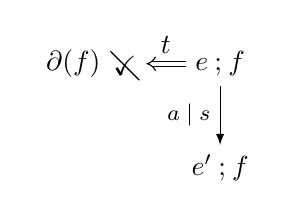
\begin{tikzpicture}[baseline=-5ex]
        \node (0) {${e}\seq{f}$};
        \node (4) [below=.75cm of 0] {${e}'{ {} \seq {f}}$};
        \node (5) [left=0.5cm of 0] {{ \bcancel\checkmark}};
            \node (5a) [left=-.2cm of 5] {{ \(\partial({f})\)}};
        \draw (0) edge[-implies, double, double distance=0.5mm] node[above] {\({t}\)} (5);
        \draw (0) edge[-latex] node[left] {\footnotesize\( {a} \mid {s}\)} (4);
\end{tikzpicture}
\end{gather*}
Intuitively, $c_{f}$ reroutes the transitions coming out of ${e}$: acceptance (the first case) is replaced by the behaviour of ${f}$, and the probability mass of transitioning to ${e}'$ (the second case) is reassigned to $ e\seq f$.
A pictorial representation of the effect on the derivatives of ${e} \seq {f}$ is given above on the right.
Here, we assume that \(\partial({e})\) can perform a \({a}\)-transition to \({e'}\) with probability \({s}\); we make the same assumption in the informal descriptions of derivatives for the loops, below. 

For loops, we require $\partial\left(e^{[p]}\right)$ to be the least subdistribution satisfying $\partial\left(e^{[p]} \right) =  p \partial(e) \lhd e^{{[p]}} + (1-p) \partial(\checkmark)$. In the case when $\partial(e)(\checkmark)\neq 0$, the above becomes a fixpoint equation (as in such a case, the unrolling of the definition of $(- \lhd e^{[p]})$ involves $\partial \left( e{[p]}\right)$). We can define $\partial \left( e^{[p]} \right)$ as a closed form, but we need to consider two cases. If $\partial(e)(\checkmark)=1$ and $p = 1$, then the loop body is constantly executed, but the inner expression $e$ does not perform any labelled transitions. We identify such divergent loops with deadlock behaviour and hence $\partial(e^{[p]})(x)=0$. Otherwise, we look at $\partial(e)$ to build $\partial\left({e}^{[p]}\right)$. First, we make sure that the loop may be skipped with probability $1-p$.
Next, we modify the branches that perform labelled transitions by adding ${e}^{[p]}$ to be executed next.
The remaining mass is $p\partial(e)(\checkmark)$, the probability that we will enter the loop and immediately exit it without performing any labelled transitions. We discard this possibility and redistribute it among the remaining branches. 
As before, we provide an informal visual depiction of the probabilistic loop semantics below, using the same conventions as before. The crossed-out checkmark along with the dashed lines denotes the redistribution of probability mass described above.
\[
	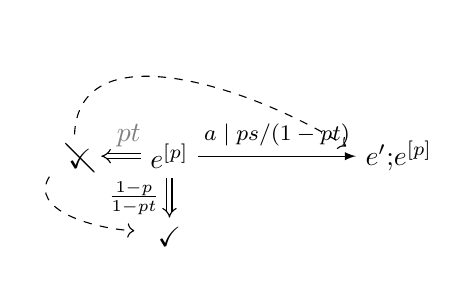
\begin{tikzpicture}
        \node (0) {${e}^{[p]}$};
        \node (6) [below=.5cm of 0] {\checkmark};
        \node (4) [right=2cm of 0] {${e}'{ \seq {e}^{[{p}]}}$};
        \node (5) [left=.5cm of 0] {{ \(\bcancel{\checkmark}\)}};
        \draw (0) edge[-implies, double, double distance=0.5mm] node[left] {\footnotesize \(\frac{1-{p}}{1-{pt}}\)} (6);
        \draw (0) edge[-implies, double, double distance=0.5mm, pos=0.3] node[above, gray] {\({pt}\)} (5);
        \draw (0) edge[-latex] node[above] {\footnotesize\( {a} \mid {{{p}}}{s}/{ (1-{pt})}\)} (4);
        \draw (5) edge[->,dashed,bend left, out=90] ($(4.west) + (-0.35,0.55)$);
        \draw (5) edge[->,dashed,bend right, out=-90] ($(6.west) + (-0.5,0.35)$);
  %      \draw[dotted,bend right=20] (5) edge[-latex] (4);
   %     \draw[dotted,bend left=20] (5) edge[-latex] (6);
    \end{tikzpicture}
\]
Formally speaking, the definition of $\partial\left({e}^{[{p}]}\right)$ can be given by the following:
\begin{gather*}
\partial\left(e^{[p]}\right)(x)= \begin{cases}
    \frac{1-p}{1-p\partial(e)(\checkmark)} & x = \checkmark \\[1.2ex]
    \frac{p\partial(e)(a,e')}{1-p\partial(e)(\checkmark)} & x = (a, (e' \seq e^{[p]}))\\
    0 & \text{otherwise}
\end{cases}
\end{gather*}
% Having defined the semantics, we can easily observe that the termination operator $E : \PExp \to \interval{0}{1}$ captures the probability of immediate acceptance.
% \begin{restatable}{lemma}{exitoperatorlemma}\label{c4:lem:exit_operator_lemma}
% For all $e \in \PExp$ it holds that $E(e)=\partial(e)(\checkmark)$
% \end{restatable}
% In our case, the canonical concept of coalgebraic bisimilarity (which in the case of {GPTS} directly corresponds to the notion from~\cite{Larsen:1991:Bisimulation}) is too discriminating notion of equivalence. For example, the states in the Brzozowski transition system for expressions $(a \oplus_{\frac{1}{2}} \zero) \seq (b \oplus_{\frac{1}{3}} \zero) $ and $(a \oplus_{\frac{1}{3}} \zero) \seq (b \oplus_{\frac{1}{2}} \zero) $ both generate a word $ab$ with probability $\frac{1}{6}$, while not being bisimilar. The state for the first expression can perform an $a$-transition with probability $\frac{1}{2}$, while the second one performs the same action with the probability of $\frac{1}{3}$, thus making them distinguished by the notion of bisimilarity.

% As mentioned before, if we omit the axioms marked with $\heartsuit$ from \cref{fig:axioms}, we obtain a coarser congruence relation ${\equiv_b} \subseteq \PExp \times \PExp$, sound wrt. coalgebraic bisimilarity. 
% % We will later use it in the proof of soundness of our axiomatisation wrt. language equivalence, as an intermediate step.
% \begin{restatable}{lemma}{soundnessbisim}\label{c4:lem:soundness_bisim}
%     The relation ${\equiv_b} \subseteq {\PExp \times \PExp}$ is a bisimulation equivalence
% \end{restatable}
% As a consequence~\cite{Rutten:2000:Universal}, there exists a unique coalgebra structure $\qcoa : {\PExp}/{\equiv_b} \to \distf \funF {\PExp}/{\equiv_b}$, which makes the quotient map $[-]_{\equiv_b} : \PExp \to {\PExp}/{\equiv_b}$ into $\distf \funF$-coalgebra homomorphism from $(\PExp, \equiv)$ to $({{\PExp}/{\equiv_b}}, \qcoa)$.

Having defined the Antimirov transition system, one can observe that the termination operator $E(-) \colon \PExp \to \interval{0}{1}$ precisely captures the probability of an expression transitioning to $\checkmark$ (successful termination) when viewed as a state in the Antimirov {GPTS}.

\begin{lemma}\label{c4:lem:exit_operator_lemma}
    For all $e \in \PExp$ it holds that $E(e)=\partial(e)(\checkmark)$.
\end{lemma}
\begin{proof}
By structural induction. The base cases $E(\zero)=0=\partial(\zero)(\checkmark)$, $E(\one)=1=\partial(\one)(\checkmark)$ and $E(a)=0=\partial(a)(\checkmark)$ hold immediately. For the inductive steps, we have the following:
\begin{itemize}
	 \item[] \fbox{Probabilistic choice}
	 	\begin{align*}
	 		E(e \oplus_p f) &= pE(e) + (1-p)E(f)\\ &= p\partial(e)(\checkmark) + (1-p)\partial(f)(\checkmark)\\ &= \partial(e \oplus_p f)(\checkmark)
	 	\end{align*}
	 \item[] \fbox{Sequential compositon}
	 \begin{align*}
	 	E(e \seq f)&=E(e)E(f)\\
	 	&=\partial(e)(\checkmark)\partial(f) (\checkmark)\\
	 	&= (\partial (e) \lhd f)(\checkmark)\\
	 	&=\partial(e \seq f)(\checkmark)
	 \end{align*}
	 \item[] \fbox{Loops} First, we consider the case when $\partial(e)(\checkmark)=1$ and the loop probability is $1$. By induction hypothesis, also $E(e)=1$ and hence $E\left(e^{[1]}\right)=\partial\left(e^{[1]}\right)(\checkmark)$. Otherwise, we have the following:
	\begin{align*}
		E(e^{[p]})&=\frac{1-p}{1-pE(e)}\\
		&=\frac{1-p}{1-p\partial(e)(\checkmark)}\\
		&=\partial\left(e^{[p]}\right)(\checkmark)
	\end{align*}
\end{itemize}
\end{proof}


Given an expression $e \in \PExp$, we write $\langle e\rangle \subseteq \PExp$ for the set of states reachable from $e$ by repeatedly applying $\partial$.
It turns out that the operational semantics of every {PRE} can be always described by a finite-state {GPTS} given by $(\langle e \rangle, \partial)$.
\begin{lemma}\label{c4:lem:locally_finite}
    For all $e \in \PExp$, the set $\langle e \rangle$ is finite. In fact, the number of of states is bounded above by $\#(-) \colon \PExp \
    \to \N$, where $\#(-)$ is defined recursively by:
    \begin{align*}
        \#(\zero)=\#(\one)=1 \quad \#(a) = 2 \quad \#(e \oplus_p f) = \#(e) + \#(f)\\ 
        \#(e \seq f) = \#(e) + \#(f) \quad \#(e^{[p]}) = \#(e) + 1
    \end{align*}
\end{lemma}
\begin{proof}
    We adapt the analogous proof for {GKAT}~\cite{Schmid:2021:Guarded}.

    For any \({e} \in \PExp\), let \(|\langle e \rangle|\) be the cardinality of the carrier set of the least subcoalgebra of \((\PExp, \partial)\) containing \(e\). We show by induction that for all \(e \in \PExp\) it holds that \(|\langle e \rangle|\leq \#({e})\).

     For the base cases, observe that for $\zero$ and $\one$ the subcoalgebra has exactly one state. Hence, \(\#(\zero) = 1 = |\langle \zero \rangle|\). Similarly, we have \(\#(\one) = 1 = |\langle \one \rangle|\).
    For \(a \in \alphabet\), we have two states; the initial state, which transitions with probability \(1\) on \(a\) to the state which outputs \(\checkmark\) with probability \(1\).

    For the inductive cases, assume that \(|\langle e \rangle| \leq \#(e)\), \(|\langle f \rangle| \leq \#(f)\) and \(p \in \interval{0}{1}\).
     \begin{itemize}
         \item
         Every derivative of \({e} \oplus_p {f}\) is either a derivative of \({e}\) or \({f}\) and hence \(|\langle e \oplus_p f \rangle| \leq |\langle e \rangle| + |\langle f \rangle| = \#({e}) + \#({f}) = \#({e} \oplus_p {f})\).
         \item
         In the case of \({e}\seq{f}\), every derivative of this expression is either a derivative of \({f}\) or some derivative of \({e}\) followed by \({f}\). Hence, \(|\langle e \seq f \rangle| = |\langle e \rangle\times \{{f}\}| + |\langle f \rangle| \leq \#({e}) + \#({f}) = \#({e}\seq{f}) \).

         \item
         For the probabilistic loop case, observe that every derivative of \({e}^{[{p}]}\) is a derivative of \({e}\) followed by \({e}^{[{p}]}\) or it is the state that outputs $\checkmark$ with probability $1$. It can be easily observed,that \(|\langle e^{[p]}\rangle| \leq |\langle e \rangle| + 1 = \#({e}) = \#({e}^{[p]})\). 
    \end{itemize}
\end{proof}



\begin{example} Operational semantics of the expression $e = a \oplus_{\frac{3}{4}} a \seq a^{[\frac{1}{4}]}\seq a$ correspond to the following {GPTS}: 
\begin{center}
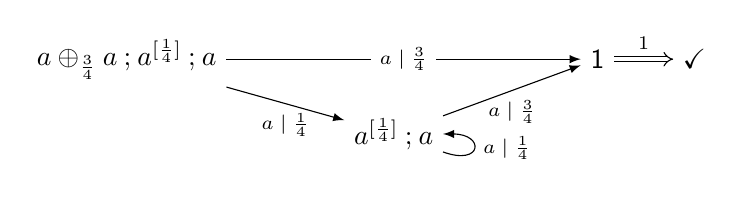
\begin{tikzpicture}%[baseline=0ex]
        \node (2) {$a \oplus_{\frac{3}{4}} a \seq a^{[\frac{1}{4}]}\seq a$};
        \node (2a) [ right= 2 cm of 2]{};
        \node (3) [below= .5 cm of 2a] {$a^{[\frac{1}{4}]}\seq a$};
        \draw (2) edge[-latex] node[below] {\scriptsize\( {a} \mid {\frac{1}{4}}\)} (3);
        \draw (3) edge[-latex,out=-20,in=0,looseness=6] node[right] {\scriptsize\( {a} \mid {\frac{1}{4}}\)} (3);
        \node (4) [right= 4.5 cm of 2] {$\one$};
        \draw (3) edge[-latex] node[below] {\scriptsize\( {a} \mid {\frac{3}{4}}\)} (4);
        \draw (2) edge[-latex] node[ fill=white] {\scriptsize\( {a} \mid {\frac{3}{4}}\)} (4);
        \node (o2) [right= 0.75 cm of 4]{$\checkmark$};
        \draw (4) edge[-implies, double, double distance=0.5mm] node[above] {\scriptsize\( 1\)} (o2);
\end{tikzpicture}
\end{center}
One can observe that the transition system above for $e$ is isomorphic to the one starting in $q_2$ in \Cref{c4:ex:systems}.
\end{example}

Given the finite-state {GPTS} $(\langle e \rangle, \partial)$ associated with an expression $e\in \PExp$ we can define the language semantics of $e$ as the probabilistic language $\llbracket e\rrbracket \in \interval{0}{1}^{\alphabet^*}$ generated by the state $e$ in the {GPTS} $(\langle e \rangle, \partial)$. 

\subsection{Roadmap to soundness and completeness}\label{c4:subsec:roadmap}
The central aim of this chapter is to show that the axioms in \Cref{c4:fig:axioms} are sound and complete to reason about probabilistic language equivalence of {PRE}, that is:
\[
e \equiv f \quad \begin{array}{c} {\text{\tiny Completeness}} \\ \Longleftarrow\\ \Longrightarrow\\ {\text{\tiny Soundness}} \end{array} \llbracket e\rrbracket = \llbracket f\rrbracket
\]
We now sketch the roadmap on how we will prove these two results to ease the flow into the upcoming technical sections. Perhaps not surprisingly, the completeness direction is the most involved. 
%However, because of the rich algebraic structure of probabilistic languages, the soundness direction is not a simple straightforward inductive proof as in the case of regular expressions. 

The heart of both arguments will rely on arguing that the semantics map $\llbracket - \rrbracket \colon \PExp \to \interval{0}{1}^{\alphabet^\ast}$ assigning a probabilistic language to each expression can be seen as the following composition of maps:
% https://q.uiver.app/#q=WzAsMyxbMCwwLCJcXEV4cCJdLFsyLDAsIntcXEV4cH0ve1xcZXF1aXZ9Il0sWzQsMCwiWzAsMV1ee0FeKn0iXSxbMCwxLCJbLV0iXSxbMSwyLCJcXGRhZ2dlciBkIl0sWzAsMiwiXFxsbGJyYWNrZXQtXFxycmJyYWNrZXQiLDIseyJjdXJ2ZSI6M31dXQ==
\[\begin{tikzcd}
	\PExp && {{\PExp}/{\equiv}} && {\interval{0}{1}^{\alphabet^*}}
	\arrow["{[-]}", from=1-1, to=1-3]
	\arrow["{\beh{d}}", from=1-3, to=1-5]
	\arrow["{\llbracket-\rrbracket}"', curve={height=20pt}, from=1-1, to=1-5]
\end{tikzcd}\] 
The tehcnical core of both arguments will rely on equipping ${\PExp}/{\equiv}$ with a structure of a $\funG$-coalgebra, possesing additional well-behaved $\pca$ structure making it into a $\overline{\funG}$-coalgebra. In the picture above $[-] \colon \PExp \to {\PExp}/{\equiv}$ is a quotient map taking expressions to their equivalence class modulo the axioms of $\equiv$, while $\beh{d} \colon {\PExp}/{\equiv} \to \interval{0}{1}^{\alphabet^\ast}$ is a final $\funG$-coalgebra homomorphism taking each equivalence class to the corresponding probabilistic language. In such a case, soundness follows as a sequence of three steps:
\begin{equation}\label{eq:sound}
 e\equiv f\Rightarrow [e]=[f] \Rightarrow \beh{d} ([e])  = \beh{d} ( [f] ) \Rightarrow \llbracket e\rrbracket = \llbracket f\rrbracket 
 \end{equation}
 In general, obtaining the appropriate transition system structure on $\PExp/_\equiv$ needs a couple of intermediate steps, which then lead to soundness:
\begin{enumerate}
\item We first prove the soundness of a subset of the axioms of \Cref{c4:fig:axioms}: omitting (\textsf{S0}) and (\textsf{D2}) yields a sound inference system, which we call $\equiv_b$, with respect to a finer equivalence--probabilistic bisimilarity as defined by Larsen and Skou~\cite{Larsen:1991:Bisimulation} (\Cref{c4:lem:soundness_bisim}). As a consequence, there exists a deterministic transition system structure on the set $\distf{{\PExp}/{\equiv_b}}$, such that $\distf [-]_{\equiv_b} \colon \distf \PExp \to \distf {{\PExp}/{\equiv_b}}$ is a $\funG$-coalgebra homomorphism (\Cref{c4:lem:homom_of_determinisations}). 
\item We then prove that the set of expressions modulo the bisimilarity axioms, that is $\PExp/_{\equiv_b}$, has the structure of a positive convex algebra $\alpha_{\equiv_b} \colon \distf{{\PExp}/{\equiv_b}} \to {\PExp}/{\equiv_b}$ (\Cref{lem:quotient_is_an_em_algebra}). This allows us to flatten a distribution over equivalence classes into a single equivalence class. This proof makes use of a {\em fundamental theorem} decomposing expressions (\Cref{c4:thm:fundamental_theorem}). Additionally, we obtain that the coarser quotient ${\PExp}/{\equiv}$ also has a $\pca$ structure (\Cref{c4:lem:coarser_quotient_is_a_pca}), that will become handy in the proof of completeness.
\item With the above result, we equip the set $\PExp/{\equiv_b}$ with a $\funG$-coalgebra structure and show that the positive convex algebra structure map on ${\PExp}/{\equiv_b}$ is also a $\funG$-coalgebra homomorphism from $\distf {\PExp}/{\equiv_b}$ into it (\Cref{c4:lem:algebra_map_coalgebra_homomorphism}). 
\item Through a simple argument (this step encapsulates the key part of the soundness argument), we show that there exists a unique deterministic transition system structure on the coarser quotient, that is ${\PExp}/{\equiv}$, that makes further identification using axioms (\textsf{S0}) and (\textsf{D2}) (denoted $[-]_{\equiv} \colon {\PExp}/{\equiv_b} \to {\PExp}/{\equiv}$) into a $\funG$-coalgebra homomorphism (\Cref{c4:lem:coalg_on_quotient_left_dist}). We compose all homomorphisms into a map of the type $\distf {\PExp} \to {\PExp}/{\equiv}$ and show the correspondence of the probabilistic language of the state $[e]$ in the above mentioned $\funG$-coalgebra with the one of $\delta_{e}$ in the determinisation of Antimirov {GPTS} (\Cref{c4:lem:factoring_lemma2}), thus establishing soundness (\Cref{c4:thm:soundness}).
\end{enumerate}
  As much as our proof of soundness is not a straightforward inductive argument like in ordinary regular expressions, it immediately sets up the stage for the completeness argument. To obtain completeness we want to reverse all implications in \Cref{eq:sound}--and they all are easily reversible except $[e]=[f] \Rightarrow \beh{d} ( [e] )  =  \beh{d} ( [f] )$. To obtain this reverse implication we will need to show that $\beh{d} $ is {\em injective}. We will do this, by showing that the (algebraically structured) coalgebra on ${\PExp}/{\equiv}$ satisfies a universal property of the rational fixpoint, that generalises the idea of regular languages representing finite-state deterministic automata. 
  
As we will see in \Cref{c4:sec:completeness}, determinising a finite-state {GPTS} can lead to an infinite state $\funG$-coalgebra. Instead, we will rely on the theory of locally finitely presentable categories to characterise finite behaviour. It turns out, each determinisation of a finite-state {GPTS} carries a structure of a positive convex algebra, that is \emph{free finitely generated}. Thanks to the work of Milius~\cite{Milius:2018:Proper} and Sokolova \& Woracek~\cite{Sokolova:2018:Proper} on \emph{proper functors}, we will see that establishing that ${\PExp}/{\equiv}$ is isomorphic to the rational fixpoint boils down to showing uniqueness of homomorphisms from determinisations of finite-state {GPTS}. We will reduce this problem to converting {GPTS} to language equivalent expressions through the means of axiomatic manipulation using a procedure reminiscent of Brzozowski's equation solving method~\cite{Brzozowski:1964:Expressions} for converting DFAs to regular expressions. As a corollary, we will obtain an analogue of (one direction of) Kleene's theorem for {GPTS} and {PRE}. To sum up, the completeness result is obtained in $4$ steps:
  
 \begin{enumerate}
\item We show that the structure map of $\funG$-coalgebra on ${\PExp}/{\equiv}$ constructed in previous step is in fact a $\pca$ homomorphism, thus making it into a $\overline{\funG}$-coalgebra (\Cref{c4:smappcahomom}). 
\item We show that determinisations of GPTS, as well as $\overline{\funG}$-coalgebra structure on ${\PExp}/{\equiv}$, are precisely coalgebras for the functor $\hat{\funG} \colon \pca \to \pca$ that is proper and a subfunctor of $\overline{\funG}$. 
\item Following a traditional pattern in completeness proofs~\cite{Salomaa:1966:Two,Backhouse:1976:Closure,Milner:1984:Complete}, we represent  {GPTS} as \emph{left-affine} systems of equations within the calculus and show that these systems have {\em unique} solutions up to provable equivalence (\Cref{c4:thm:unique_solutions}).
\item We then show that these solutions are in 1-1 correspondence with well-behaved maps from $\hat{\funG}$-coalgebras obtained from determinising finite-state {GPTS} into the $\hat{\funG}$-coalgebra on ${\PExp}/{\equiv}$ (\Cref{c4:lem:determinisations_correspond_to_df_coalgebras}). 
\item Finally, we use this correspondence together with an abstract categorical argument to show that $\hat{\funG}$-coalgebra structure on ${\PExp}/{\equiv}$ has a universal property of the rational fixpoint (\Cref{c4:cor:fully_abstract}) that eventually implies injectivity of $\beh{d}$, establishing completeness (\Cref{c4:thm:completeness}). 
\end{enumerate}
 \section{Soundness}\label{c4:sec:soundness}
We are now ready to execute the roadmap to soundness described in \Cref{c4:subsec:roadmap}. 
 \subsection{Step 1: Soundness with respect to bisimilarity}
 We first check that a subset of axioms generating $\equiv$ is sound with respect to bisimilarity of $\distf \funF$-coalgebras, which is a coarser notion of equivalence than probabilistic language equivalence. Let ${\equiv_b} \subseteq {\PExp \times \PExp}$ denote the least congruence relation closed under the axioms on \Cref{c4:fig:axioms} except (\textsf{S0}) and (\textsf{D2}). We will use the following notation for the quotient maps associated with $\equiv$ and $\equiv_b$:
% https://q.uiver.app/#q=WzAsMyxbMCwwLCJcXFBFeHAiXSxbMiwwLCJ7XFxQRXhwfS97XFxlcXVpdl9ifSJdLFs0LDAsIlxcUEV4cC97XFxlcXVpdn0iXSxbMCwxLCJbLV1fe1xcZXF1aXZfYn0iLDJdLFsxLDIsIlstXV97XFxlcXVpdn0iLDJdLFswLDIsIlstXSIsMCx7ImN1cnZlIjotNH1dXQ==
\[\begin{tikzcd}
	\PExp && {{\PExp}/{\equiv_b}} && {\PExp/{\equiv}}
	\arrow["{[-]_{\equiv_b}}"', from=1-1, to=1-3]
	\arrow["{[-]}", curve={height=-24pt}, from=1-1, to=1-5]
	\arrow["{[-]_{\equiv}}"', from=1-3, to=1-5]
\end{tikzcd}\]

A straightforward induction on the length derivation of $\equiv_b$ allows us to show that this relation is a bisimulation equivalence on $(\PExp, \partial)$. As mentioned before, in the case of {GPTS} this notion corresponds to bisimulation equivalences in the sense of Larsen and Skou~\cite{Larsen:1991:Bisimulation}.  Due to readability concerns, the proof of that result is delegated to \Cref{apx:soundness}.
\begin{restatable}{lemma}{soundnessbisim}\label{c4:lem:soundness_bisim}
    The relation ${\equiv_b} \subseteq {\PExp \times \PExp}$ is a bisimulation equivalence.
 \end{restatable}
As a consequence of \Cref{c4:lem:soundness_bisim} and \Cref{c2:lem:quotient_coalgebra}, there exists a unique coalgebra structure $\qcoa \colon {\PExp}/{\equiv_b} \to \distf \funF {\PExp}/{\equiv_b}$, which makes the quotient map $[-]_{\equiv_b} \colon \PExp \to {\PExp}/{\equiv_b}$ into a $\distf \funF$-coalgebra homomorphism from $(\PExp, \partial)$ to $({{\PExp}/{\equiv_b}},\qcoa)$. It turns out, that upon converting those $\distf \funF$-coalgebras to $\funG \distf$-coalgebras using the natural transformation $\rho \colon \distf \funF \to \funG \distf$ and determinising them, $\distf [-]_{\equiv_b} \colon \distf \PExp \to \distf {\PExp}/{\equiv_b}$ becomes a homomorphism between the determinisations. 
\begin{lemma}\label{c4:lem:homom_of_determinisations}
	$\distf [-]_{\equiv_b} \colon \distf \PExp \to \distf {\PExp}/{\equiv_b}$ is a $\funG$-coalgebra homomorphism from $(\distf \PExp, (\rho_{\PExp} \circ \partial)^\sharp)$ to  $(\distf {\PExp}/{\equiv_b}, (\rho_{{\PExp}/{\equiv_b}} \circ \qcoa)^\sharp)$. In other words, the following diagram commutes:
% https://q.uiver.app/#q=WzAsOCxbMCwxLCJcXFBFeHAiXSxbMCwyLCJcXGRpc3RmIFxcZnVuRiBcXFBFeHAiXSxbMCwzLCJcXGZ1bkdcXGRpc3RmIFxcUEV4cCJdLFsxLDAsIlxcZGlzdGYgXFxQRXhwIl0sWzIsMSwiXFxQRXhwL3tcXGVxdWl2X2J9Il0sWzMsMCwiXFxkaXN0ZiB7e1xcUEV4cH0ve1xcZXF1aXZfYn19Il0sWzIsMywiXFxmdW5HXFxkaXN0ZiB7XFxQRXhwfS97XFxlcXVpdl9ifSJdLFsyLDIsIlxcZGlzdGYgXFxmdW5GIHtcXFBFeHB9L3tcXGVxdWl2X2J9Il0sWzAsMSwiXFxwYXJ0aWFsIiwyXSxbMSwyLCJcXGdhbW1hX3tcXFBFeHB9IiwyXSxbMCwzLCJcXGV0YV97XFxQRXhwfSIsMCx7ImxhYmVsX3Bvc2l0aW9uIjo0MH1dLFs0LDUsIlxcZXRhX3t7XFxQRXhwfS97XFxlcXVpdl9ifX0iLDAseyJsYWJlbF9wb3NpdGlvbiI6MTB9XSxbMyw1LCJcXGRpc3RmIFstXV97XFxlcXVpdl9ifSJdLFswLDQsIlstXV97XFxlcXVpdl9ifSIsMl0sWzQsNywiXFxxY29hIiwyXSxbNyw2LCJcXGdhbW1hX3t7XFxQRXhwfS97XFxlcXVpdl9ifX0iLDJdLFsyLDYsIlxcZnVuRyBcXGRpc3RmIFstXV97XFxlcXVpdl9ifSJdLFszLDIsIihcXGdhbW1hX3tcXFBFeHB9IFxcY2lyYyBcXHBhcnRpYWwpXlxcc2hhcnAiLDAseyJjdXJ2ZSI6LTN9XSxbNSw2LCIoXFxnYW1tYV97e1xcUEV4cH0ve1xcZXF1aXZfYn19IFxcY2lyYyBcXHFjb2EpXlxcc2hhcnAiLDAseyJjdXJ2ZSI6LTR9XV0=
\[\begin{tikzcd}
	& {\distf \PExp} && {\distf {{\PExp}/{\equiv_b}}} \\
	\PExp && {\PExp/{\equiv_b}} \\
	{\distf \funF \PExp} && {\distf \funF {\PExp}/{\equiv_b}} \\
	{\funG\distf \PExp} && {\funG\distf {\PExp}/{\equiv_b}}
	\arrow["{\distf [-]_{\equiv_b}}", from=1-2, to=1-4]
	\arrow["{(\gamma_{\PExp} \circ \partial)^\sharp}", curve={height=-18pt}, from=1-2, to=4-1]
	\arrow["{(\gamma_{{\PExp}/{\equiv_b}} \circ \qcoa)^\sharp}", curve={height=-24pt}, from=1-4, to=4-3]
	\arrow["{\eta_{\PExp}}"{pos=0.4}, from=2-1, to=1-2]
	\arrow["{[-]_{\equiv_b}}"', from=2-1, to=2-3]
	\arrow["\partial"', from=2-1, to=3-1]
	\arrow["{\eta_{{\PExp}/{\equiv_b}}}"{pos=0.1}, from=2-3, to=1-4]
	\arrow["\qcoa"', from=2-3, to=3-3]
	\arrow["{\gamma_{\PExp}}"', from=3-1, to=4-1]
	\arrow["{\gamma_{{\PExp}/{\equiv_b}}}"', from=3-3, to=4-3]
	\arrow["{\funG \distf [-]_{\equiv_b}}", from=4-1, to=4-3]
\end{tikzcd}\]
\end{lemma}
\begin{proof}
	Front face of the diagram commutes because $[-]_{\equiv_b}$ is $\distf \funF$-coalgebra homomorphism and because of \cite[Theorem~15.1]{Rutten:2000:Universal}. The sides of the diagram commute because of the free-forgetful adjunction between $\Set$ and $\pca$. Finally, the commutativity of the square at the back of the diagram above follows from \cite[Theorem~4.1]{Silva:2010:Generalizing}.
\end{proof}
\subsection{Step 2a: Fundamental theorem}  We show that every PRE is provably equivalent (modulo the axioms of $\equiv_b$) to a decomposition involving sub-expressions obtained in its small-step semantics. This property, often referred to as the fundamental theorem (in analogy with the fundamental theorem of calculus) is useful in proving soundness. In order to encode elements of $\funF \PExp$ using the syntax of $\PExp$, we define a function $\ex \colon \funF \PExp \to \PExp$, given by $\ex(\checkmark)=1$ and $\ex(a,e')=a;e'$ for all $a \in \alphabet$ and $e' \in \PExp$. To be able to syntactically express finitely supported subdistributions, we will use $n$-ary convex sum of elements of $\PExp$ obeying the axioms of positive convex algebras, that exists because of \Cref{c4:prop:binary} and axioms (\textsf{C1-C4}). Using it, we can state the following:

\begin{restatable}{theorem}{fundamentaltheorem}\label{c4:thm:fundamental_theorem}
    For all $e \in \PExp$ we have that 
    $$
    e \equiv_b \bigoplus_{d \in \supp(\partial(e))} \partial(e)(d) \cdot \ex(d)
    $$
\end{restatable}
Before we give the proof of the result above, we start by establishing a couple of intermediate results. Firstly, we show that the binary probabilistic choice satisfies the following identities:
\begin{lemma}\label{c4:lem:binary_sum_properties}
    The following facts are derivable in $\equiv_b$
    \begin{enumerate}
        \item $e \oplus_p (f 
        \oplus_q g) \equiv_b \left( e \oplus_{\frac{p}{1-(1-p)(1-q)}} f \right) \oplus_{1-(1-p)(1-q)} g $
        \item $(e \oplus_p f) \oplus_q (g \oplus_p h) \equiv_b (e \oplus_q g) \oplus_p (f \oplus_q h)$
    \end{enumerate}
\end{lemma}
\begin{proof}
For \circlednum{1}, let $k = \frac{p}{1-(1-p)(1-q)} $ and $l = 1-(1-p)(1-q)$. We derive the following:
    \begin{align*}
        e \oplus_p (f \oplus_q g) &\equiv_b  (f \oplus_q g) \oplus_{1-{p}} e \tag{\textsf{C3}} \\
        &\equiv_b (g \oplus_{1-{q}} f) \oplus_{1-{p}} e \tag{\textsf{C3}} \\
        &\equiv_b g \oplus_{1-{l}} (f \oplus_{1-{k}} e) \tag{\textsf{C4}} \\
        &\equiv_b (f \oplus_{1-{k}} e) \oplus_{{l}} g\tag{\textsf{C3}} \\
        &\equiv_b (e \oplus_{{k}} f) \oplus_{{l}} g\tag{\textsf{C3}} \\
    \end{align*}
For \circlednum{2} we show the following:
    \begin{align*}
        (e \oplus_p f) \oplus_q (g \oplus_p h) &\equiv_b e \oplus_{pq} \left(f \oplus_{\frac{1-{p}q}{1-pq}} (g \oplus_p h)\right) \tag{\textsf{C4}}\\
        &\equiv_b e \oplus_{pq} \left((g \oplus_p h) \oplus_{\frac{1-{q}}{1-pq}} f \right) \tag{\textsf{C3}} \\
        &\equiv_b e \oplus_{pq} \left(g \oplus_{\frac{p(1-{q})}{1-pq}} \left(h \oplus_{1-{q}} f\right) \right) \tag{\textsf{C4}} \\
        &\equiv_b e \oplus_{pq} \left(g \oplus_{\frac{p(1-{q})}{1-pq}} \left(f \oplus_{{q}} h\right) \right) \tag{\textsf{C3}}\\
        &\equiv_b \left(e \oplus_q g\right) \oplus_p \left(f \oplus_q h\right) \tag{\circlednum{1}}
    \end{align*}

\end{proof}



Then, we argue that any non-empty $n$-ary convex sum can be expressed as a binary probabilistic choice and an $(n-1)$-nary convex sum.
\begin{lemma}\label{c4:lem:sum_unrolling}
    Let $\{p_i\}_{i \in I}$ and $\{e_i\}_{i \in I}$ be non-empty collections indexed by a finite set $I$, such that for all $i \in I$, $p_i \in \interval{0}{1}$ and $e_i \in \PExp$. For any $j \in I$ it holds that:
    \[
        \bigoplus_{i \in I} p_i \cdot e_i \equiv_b e_j \oplus_{p_j} \left(\bigoplus_{i \in I \setminus \{j\}} \frac{p_i}{1-{p_j}}\cdot e_i\right) 
    \]
\end{lemma}
\begin{proof}
    In the edge case, when $p_j = 1$ (and therefore $I = \{j\}$) we have that $\bigoplus_{i \in I} p_i \cdot e _i \equiv_b e_j$ and therefore
    \begin{align*}
        e_j &\equiv_b e_j \oplus_1 0 \tag{\textsf{C2}} \\
        &\equiv_b e_j \oplus_{p_j} \left( \bigoplus_{i \in \emptyset} \frac{p_i}{{1-p_j}} \cdot e_i \right) \tag{Def. of empty $n$-ary convex sum}\\
        &\equiv_b e_j \oplus_{p_j} \left( \bigoplus_{i \in I \setminus \{j\}} \frac{p_i}{{1-p_j}} \cdot e_i \right) \tag{$I = \{j\}$}\\
    \end{align*}
    Note that despite the fact that ${p_j} = 1$, the $n$-ary sum on the right is well-defined as it ranges over an empty index set and thus division by zero never happens. The remaining case, when $p_j \neq 1$ holds because of \Cref{c4:prop:binary}.
\end{proof}
Using the above result, we can also split the normal form used in \Cref{c4:thm:fundamental_theorem} into two parts; one describing acceptance and one describing labelled transitions.
\begin{lemma}\label{c4:lem:safe_unrolling_lemma}
    For all $e \in \PExp$, 
    $$
    \bigoplus_{d \in \supp(\partial(e))} \partial(e)(d) \cdot \ex(d) \equiv_b \one \oplus_{\partial(e)(\checkmark)} \left(\bigoplus_{d \in \supp(\partial(e)) \setminus \{\checkmark\}} \frac{\partial(e)(d)}{1-{\partial(e)(\checkmark)}} \cdot \ex(d)\right)
    $$
\end{lemma}
\begin{proof}
    If $\supp(\partial(e)) = \emptyset$, then 
    \begin{align*}
        \bigoplus_{d \in \supp(\partial(e))} \partial(e)(d) \cdot \ex(d) &\equiv_b \zero \tag{Def. of empty $n$-ary convex sum}\\
        &\equiv_b 0 \oplus_1 1 \tag{\textsf{C2}} \\
        &\equiv_b 1 \oplus_0 0 \tag{\textsf{C3}} \\
        &\equiv_b 1 \oplus_{\partial(e)(\checkmark)} 0 \tag{$\partial(e)(\checkmark)=0$}\\
        &\equiv_b 1 \oplus_{\partial(e)(\checkmark)} \left( 
            \bigoplus_{d \in \emptyset } \frac{\partial(e)(d)}{1-{\partial(e)(\checkmark)}} \cdot \ex (d)\right)\\ 
        &\equiv_b 1 \oplus_{\partial(e)(\checkmark)} \left( 
                \bigoplus_{d \in \supp(\partial(e)(\checkmark))\setminus \{\checkmark\} } \frac{\partial(e)(d)}{1-{\partial(e)(\checkmark)}} \cdot \ex(d)\right)\\ 
    \end{align*}
    
    The remaining case when $\supp(\partial(e)) \neq 0$ holds by \Cref{c4:lem:sum_unrolling} and the fact that $\ex(\checkmark) = 1$.
\end{proof}
Finally, we generalise the axiom (\textsf{D1}) to $n$-ary convex sums.
\begin{lemma}\label{c4:lem:generalised_right_distributivity}
    Let $f \in \PExp$, $I$ be a finite index set and let $\{p_i\}_{i \in I}$ and $\{e_i\}_{i \in I}$ indexed collections of probabilities and expressions respectively. Then,
    $$\left(\bigoplus_{i \in I} p_i \cdot e_i\right) \seq f \equiv_b \bigoplus_{i \in I} p_i \cdot e_i \seq f$$
\end{lemma}
\begin{proof}
    By induction. If $I = \emptyset$, then using (\textsf{0S}) we can show that
    \[
        \left(\bigoplus_{i \in I} p_i \cdot e_i\right) \seq f \equiv_b \zero \seq f \equiv_b \zero \equiv_b \bigoplus_{i \in I} p_i \cdot e_i \seq f 
    \]
    If there exists $j \in I$, such that $p_j = 1$, then
    \[
        \left(\bigoplus_{i \in I} p_i \cdot e_i\right) \seq f \equiv_b e_j \seq f\equiv_b \left(\bigoplus_{i \in I} p_i \cdot e_i \seq f\right)
    \]
    Finally, for the induction step, we have that
    \begin{align*}
         \left(\bigoplus_{i \in I} p_i \cdot e_i\right) \seq f &\equiv_b \left( e_j \oplus_{p_j} \left(\bigoplus_{i \in I \setminus \{j\}} \frac{p_i}{{1-p_j}} \cdot e_i\right) \right) \seq f \\
         &\equiv_b  e_j\seq f \oplus_{p_j} \left(\bigoplus_{i \in I \setminus \{j\}} \frac{p_i}{1-{p_j}} \cdot e_i\right)\seq f \tag{\textsf{D1}} \\
         &\equiv_b  e_j\seq f \oplus_{p_j} \left(\bigoplus_{i \in I \setminus \{j\}} \frac{p_i}{1-{p_j}} \cdot e_i\seq f\right) \tag{Induction hypothesis}\\
         &\equiv_b \left(\bigoplus_{i \in I} p_i \cdot e_i \seq f\right)
    \end{align*}
\end{proof}
We now have all the ingredients to show the fundamental theorem. 
\begin{proof}[Proof of \Cref{c4:thm:fundamental_theorem}]
	We proceed by the structural induction on $e \in \PExp$. For the base cases, we have the following:
	 \begin{itemize}
        \item[]\fbox{$e = \zero$}
        \begin{align*}
            \zero &\equiv_b \bigoplus_{d \in \emptyset} \partial(\zero)(d) \cdot \ex(d) \tag{\Cref{c4:prop:properties_of_positive_convex_algebras}}\\
            &\equiv_b \bigoplus_{d \in \supp(\partial(\zero))} \partial(\zero)(d) \cdot \ex(d) \tag{$\supp(\partial(\zero))=\emptyset$}\\
        \end{align*}
        \item[]\fbox{$e=\one$}
        \begin{align*}
            \one &\equiv_b \ex(\checkmark) \tag{Def. of $\ex$}\\ 
            &\equiv_b \bigoplus_{d \in \supp(\partial(\one))} \partial(\one)(d) \cdot \ex (d) \tag{$\partial(\one) = \delta_{\checkmark} $}
        \end{align*}
        \item[]\fbox{$e = a$}
        \begin{align*}
            a &\equiv_b a \seq \one \tag{\textsf{S1}}\\ 
            &\equiv_b \ex((a,\checkmark)) \tag{Def. of $\ex$}\\
            &\equiv_b \bigoplus_{d \in \supp(\partial(a))} \partial(a)(d) \cdot \ex (d) \tag{$\partial(a) = \delta_{(a, \checkmark)}$}
        \end{align*}
    \end{itemize}
    We now move on to inductive steps.
    \begin{itemize}
        \item[]\fbox{$e = f \oplus_p g $}
        {
        \small
        \begin{align*}
            f \oplus_p g &\equiv_b \left( \bigoplus_{d \in \supp(\partial(f))} \partial(f)(d) \cdot \ex(d) \right)\oplus_p  \left( \bigoplus_{d \in \supp(\partial(g))} \partial(g)(d) \cdot \ex(g) \right) \tag{Induction hypothesis}\\
            &\equiv_b \left( \bigoplus_{d \in \supp(\partial(f \oplus_p g))}\partial(f)(d) \cdot \ex(d) \right) \oplus_p  \left( \bigoplus_{d \in \supp(\partial(f \oplus_p g))} \partial(g)(d) \cdot \ex(g) \right) \tag{\Cref{c4:prop:properties_of_positive_convex_algebras}}\\
            &\equiv_b \bigoplus_{d \in \supp(\partial(f \oplus_p g))} \left(p\partial(f)(d) + {(1-p)}\partial(g)(d)\right) \cdot \ex(d) \tag{Barycenter axiom}\\
             &\equiv_b \bigoplus_{d \in \supp(\partial(f \oplus_p g))} \partial(f \oplus_p g)(d) \cdot \ex(d) \tag{Def. of $\partial$}
        \end{align*}
        }
        \item[]\fbox{$e = f\seq g $}
        {
        \small
        \begin{align*}
            f \seq g &\equiv_b \left(\bigoplus_{d \in \supp(\partial(f))} \partial(f)(d) \cdot \ex(d) \right) \seq g \tag{Induction hypothesis} \\
            &\equiv_b \left(\one \oplus_{\partial(f)(\checkmark)} \left(\bigoplus_{d \in \supp(\partial(f)) \setminus \{\checkmark\}} \frac{\partial(f)(d)}{{1-\partial(f)(\checkmark)}} \cdot \ex(d) \right) \right) \seq g \tag{\Cref{c4:lem:safe_unrolling_lemma}}\\
            &\equiv_b \left(\one\seq g \oplus_{\partial(f)(\checkmark)} \left(\bigoplus_{d \in \supp(\partial(f)) \setminus \{\checkmark\}} \frac{\partial(f)(d)}{{1-\partial(f)(\checkmark)}} \cdot \ex(d)  \right)\seq g \right) \tag{\textsf{D1}}\\
            &\equiv_b g \oplus_{\partial(f)(\checkmark)} \left(\bigoplus_{d \in \supp(\partial(f)) \setminus \{\checkmark\}} \frac{\partial(f)(d)}{{1-\partial(f)(\checkmark)}} \cdot \ex(d)\seq g  \right)\\ \tag{\Cref{c4:lem:generalised_right_distributivity} and \textsf{1S}} \\
            &\equiv_b \left(\bigoplus_{d \in \supp(\partial(g))}\partial(g)(d) \cdot \ex(d)\right)\\&\quad\quad\quad\quad \oplus_{\partial(f)(\checkmark)} \left(\bigoplus_{d \in \supp(\partial(f)) \setminus \{\checkmark\}} \frac{\partial(f)(d)}{{1-\partial(f)(\checkmark)}} \cdot \ex(d)\seq g  \right) \tag{Induction hypothesis}\\
            &\equiv_b\left( \bigoplus_{d \in \supp(\partial(f \seq g))}\partial(g)(d) \cdot \ex(d)\right)\\&\quad\quad\quad\quad  \oplus_{\partial(f)(\checkmark)}  \left(\bigoplus_{d \in \supp(\partial(f)) \setminus \{\checkmark\}} \frac{\partial(f)(d)}{{1-\partial(f)(\checkmark)}} \cdot \ex(d)\seq g \right) \tag{\Cref{c4:prop:properties_of_positive_convex_algebras}}
        \end{align*}
        }
        Now, we simplify the subexpression on the right part of the convex sum. Define
        $n \colon F \PExp \to \interval{0}{1}$ to be: 
        $$n(d) = \begin{cases}
            \partial(f)(a, f') & d = (a, f' \seq g) \\
            0 & \text{otherwise}
        \end{cases}$$
    	By applying \Cref{c4:prop:properties_of_positive_convex_algebras} and the preceding definition, it follows that:
        \begin{align*}
            \bigoplus_{d \in \supp(\partial(f)) \setminus \{\checkmark\}} \frac{\partial(f)(d)}{{1-\partial(f)(\checkmark)}} \cdot \ex(d)\seq g &\equiv_b \bigoplus_{d \in \supp(\partial(f \seq g))} \frac{n(d)}{{1-\partial(f)(\checkmark)}} \cdot \ex(d)
        \end{align*}
       	By combining this with the previous derivation and applying the barycenter axiom, we can conclude that $$f \seq g \equiv_b \bigoplus_{d \in \supp(\partial(f \seq g))} \left(\partial(f)(\checkmark)\partial(g)(d) + n(d)\right) \cdot \ex(d) $$
       	Combining it with the previous derivation, using the barycenter axiom, we can show that:
        $$f \seq g \equiv_b \bigoplus_{d \in \supp(\partial(f \seq g))} \left(\partial(f)(\checkmark)\partial(g)(d) + n(d)\right) \cdot \ex(d) $$
       	Observe that for $d = (a, f' \seq g)$, we obtain
        $$\partial(f)(\checkmark)\partial(g)(d) + n(d) = \partial(f)(\checkmark)\partial(g)(a, f' \seq g) + \partial(f)(a, f') = \partial(f \seq g)(d)$$
        When $d = \checkmark$,  it follows that
        $$\partial(f)(\checkmark)\partial(g)(d) + n(d) = \partial(f)(\checkmark)\partial(g)(d) = \partial(f \seq g)(d)$$
    	In all remaining cases, both functions assign the value $0$ to $d$. Consequently, we conclude that
        $$f \seq g \equiv_b \bigoplus_{d \in \supp(\partial(f \seq g))} \partial(f \seq g)(d) \cdot \ex(d)$$
        which establishes the desired result for this case.

        \item[] \fbox{$e = f^{[p]}$}
        
        We begin by considering the case where $\partial(f)(\checkmark) = 1$ and $p = 1$. 
        \begin{align*}
            f^{[p]} &\equiv_b \left(\bigoplus_{d \in \supp(\partial(f))} \partial(f)(d) \cdot \ex(d) \right)^{[1]} \tag{Induction hypothesis}\\
            &\equiv_b \one^{[1]} \tag{$\partial(f)(\checkmark)=1$}\\
            &\equiv_b \zero \tag{\textsf{Div}}\\
            &\equiv_b \bigoplus_{d \in \supp \left(\partial\left(f^{[1]}\right)\right)} \partial\left(f^{[1]}\right)(d) \cdot \ex(d)
        \end{align*}
        Otherwise, we first apply the (\textsf{Tight}) axiom to the loop body as follows:
        {
        \small
        \begin{align*}
            f^{[p]} &\equiv_b \left(\bigoplus_{d \in \supp(\partial(f))} \partial(f)(d)\cdot \ex(d)\right)^{[p]} \tag{Induction hypothesis} \\
            &\equiv_b \left(\one \oplus_{\partial(f)(\checkmark)} \left( \bigoplus_{d \in \supp(\partial(f)) \setminus \{\checkmark\}} \frac{\partial(f)(d)}{{1-\partial(f)(\checkmark)}}\cdot \ex(d)\right)\right)^{[p]} \tag{\Cref{c4:lem:safe_unrolling_lemma}}\\
            &\equiv_b \left(\left( \bigoplus_{d \in \supp(\partial(f)) \setminus \{\checkmark\}} \frac{\partial(f)(d)}{{1-\partial(f)(\checkmark)}}\cdot \ex(d)\right) \oplus_{1-{\partial(f)(\checkmark)}} \one\right)^{[p]} \tag{\textsf{C3}}\\
            &\equiv_b \left(\bigoplus_{d \in \supp(\partial(f)) \setminus \{\checkmark\}} \frac{\partial(f)(d)}{{1-\partial(f)(\checkmark)}} \cdot \ex(d)\right)^{\left[\frac{{(1-\partial(f)(\checkmark))}p}{1-p\partial(f)(\checkmark)}\right]} \tag{\textsf{Tight}}\\
        \end{align*}
        }
        For convenience, we denote by $g^{[r]}$ the expression obtained from the preceding derivation. We proceed by applying the (\textsf{Unroll}) axiom.
        {
        \small
        \begin{align*}
            g^{[r]}&\equiv_b \left(\bigoplus_{d \in \supp(\partial(f)) \setminus \{\checkmark\}} \frac{\partial(f)(d)}{{1-\partial(f)(\checkmark)}} \cdot \ex(d)\right)\seq g^{[r]} \oplus_{r} \one \tag{\textsf{Unroll}}\\
            &\equiv_b \left(\bigoplus_{d \in \supp(\partial(f)) \setminus \{\checkmark\}} \frac{\partial(f)(d)}{{1-\partial(f)(\checkmark)}} \cdot \ex(d)\right)\seq f^{[p]} \oplus_r \one \tag{$f^{[p]} \equiv_b g^{[r]}$}\\
            &\equiv_b \left(\bigoplus_{d \in \supp(\partial(f)) \setminus \{\checkmark\}} \frac{\partial(f)(d)}{{1-\partial(f)(\checkmark)}} \cdot \ex(d)\seq f^{[p]}\right) \oplus_r \one \tag{\Cref{c4:lem:generalised_right_distributivity}} \\
            &\equiv_b \left(\bigoplus_{d \in \supp(\partial(f)) \setminus \{\checkmark\}} \frac{\partial(f)(d)}{{1-\partial(f)(\checkmark)}} \cdot \ex(d)\seq f^{[p]}\right)\\&\quad\quad\quad\oplus_r \left(\bigoplus_{d \in \supp \left(\partial\left(f^{[p]}\right)\right)} \delta_{\checkmark}(d) \cdot \ex(d)\right)
        \end{align*}
        }
       Next, we simplify the left-hand side of the binary convex sum. Define $n \colon F \PExp \to \interval{0}{1}$ as follows
        $$n(d) = \begin{cases}
            {\partial(f)(a,f')} & d = \left(a, f' \seq f^{[p]}\right) \\
            0 & \text{otherwise}
        \end{cases}$$
        By applying \Cref{c4:prop:properties_of_positive_convex_algebras} and the definition above, we obtain
        {
        \small
        $$
            \bigoplus_{d \in \supp(\partial(f)) \setminus \{\checkmark\}} \frac{\partial(f)(d)}{{1-\partial(f)(\checkmark)}} \cdot \ex(d)\seq f^{[p]} \equiv_b \bigoplus_{d \in \supp \left(\partial\left(f^{[p]}\right)\right)} \frac{n(d)}{{1-\partial(f)(\checkmark)}} \cdot \ex(d)
        $$
        }
        By combining the above with the previous derivation and applying the barycenter axiom, we obtain:
        $$
        f^{[p]} \equiv_b \bigoplus_{d \in \supp \left(\partial\left(f^{[p]}\right)\right)} \left(\frac{pn(d)}{1-p\partial(f)(\checkmark)} + \frac{1-p\delta_{\checkmark}(d)}{1-\partial(f)(\checkmark)p}\right) \cdot \ex(d)
        $$
       Observe that for $d = (a, f' \seq g)$, we obtain
        $$\frac{pn(d)}{1-p\partial(f)(\checkmark)} + \frac{1-p\delta_{\checkmark}(d)}{1-p\partial(f)(\checkmark)} = \frac{p\partial(f)(a,f')}{1-p\partial(f)(\checkmark)}  = \partial \left(f^{[p]}\right)(d)$$ 
        When $d = \checkmark$,  it follows that
        $$\frac{pn(d)}{1-p\partial(f)(\checkmark)} + \frac{1-p\delta_{\checkmark}(d)}{1-p\partial(f)(\checkmark)} = \frac{1-p}{1-p\partial(f)(\checkmark)} = \partial \left(f^{[p]}\right)(d)$$
       	In all remaining cases, we have that
        $$\frac{pn(d)}{1-p\partial(f)(\checkmark)} + \frac{1-p\delta_{\checkmark}(d)}{1-p\partial(f)(\checkmark)} = 0 = \partial \left(f^{[p]}\right)(d)$$
        Thus, we obtain the following:
        $$f^{[p]}\equiv_b \bigoplus_{d \in \supp \left(\partial \left(f^{[p]}\right)\right)} \partial\left(f^{[p]}\right)(d) \cdot \ex(d)$$
        This establishes the desired result.
    \end{itemize}
\end{proof}
A direct corollary of the result established above is that every loop is provably equivalent to a loop whose body does not assign any probability to transitions to $\checkmark$.
\begin{corollary}[Productive loop]\label{c4:cor:productive_loop}
    Let $e \in \PExp$ and $p \in \interval{0}{1}$. We have that $e^{[p]} \equiv_b f^{[r]}$ for some $f \in \PExp$ and $r \in \interval{0}{1}$, such that $E(f)=0$.
\end{corollary}
\begin{proof}
    If $\partial(e)(\checkmark)=1$ and $p=1$, then it follows that:
    \begin{align*}
        e^{[1]} &\equiv_b \left(\bigoplus_{d \in \supp(\partial(e))} \partial(e)(d) \cdot \ex(d)\right)^{[1]} \tag{\Cref{c4:thm:fundamental_theorem}}\\
        &\equiv_b \one^{[1]} \\
        &\equiv_b \zero \tag{\textsf{Div}}\\
        &\equiv_b \zero\seq \zero \oplus_1 \one \tag{\textsf{0S} and \textsf{C2}}\\
        &\equiv_b \zero^{[1]} \tag{\textsf{Unique} fixpoint rule and $E(\zero)=0$}
    \end{align*}
    Therefore, $e^{[1]}=\zero^{[1]}$. In this case, it follows that $E(\zero)=0$.
    In the remaining cases, we obtain the following:
    \begin{align*}
        e^{[p]} &\equiv_b \left(\bigoplus_{d \in \supp(\partial(e))} \partial(e)(d) \cdot \ex(d)\right)^{[p]} \tag{\Cref{c4:thm:fundamental_theorem}}\\
        &\equiv_b \left(\one \oplus_{\partial(e)(\checkmark)} \left(\bigoplus_{d \in \supp(\partial(e)) \setminus \{\checkmark\}} \frac{\partial(e)(d)}{{1-\partial(e)(\checkmark)}} \cdot \ex(d)\right)\right)^{[p]} \tag{\Cref{c4:lem:safe_unrolling_lemma}} \\
        &\equiv_b \left(\left(\bigoplus_{d \in \supp(\partial(e)) \setminus \{\checkmark\}} \frac{\partial(e)(d)}{{1-\partial(e)(\checkmark)}} \cdot \ex(d)\right)\oplus_{{1-\partial(e)(\checkmark)}}  \one\right)^{[p]} \tag{\textsf{C3}}\\
        &\equiv_b \left(\left(\bigoplus_{(a,e') \in \supp(\partial(e))} \frac{\partial(e)(a,e')}{{1-\partial(e)(\checkmark)}} \cdot a \seq e'\right)\oplus_{{1-\partial(e)(\checkmark)}}  \one\right)^{[p]} \tag{Def. of $\ex$}\\
        &\equiv_b \left(\bigoplus_{(a,e') \in \supp(\partial(e))} \frac{\partial(e)(a,e')}{{1-\partial(e)(\checkmark)}} \cdot a \seq e' \right)^{\left[\frac{p{(1-\partial(e)(\checkmark))}}{1-p\partial(e)(\checkmark)}\right]} \tag{\textsf{Tight}}
    \end{align*}
Observe that the body of the loop above is an $n$-ary probabilistic sum involving terms of the form $a \seq e'$ (where $a \in \alphabet$, $e' \in \PExp$), for which $E(a \seq e') = 0$. By examining the definition of the $n$-ary sum (\Cref{c4:prop:binary}) and the termination operator $E(-)$ (\Cref{c4:fig:axioms}), we immediately conclude that the loop body is mapped to $0$ by $E(-)$, which completes the proof.
\end{proof}
\subsection{Step 2b: Algebra structure}
Then, we equip the set ${\PExp}/{\equiv_b}$ with a $\pca$ structure. To do so, we first observe that as a consequence of \Cref{c4:thm:fundamental_theorem}, we have that $\qcoa \colon {\PExp}/{\equiv_b} \to \distf \funF {\PExp}/{\equiv_b}$ is an isomorphism.
\begin{corollary}\label{c4:cor:quotient_coalgebra_inverse}
    The structure map $\qcoa : {\PExp}/{\equiv_b} \to \distf \funF {\PExp}/{\equiv_b}$ of the quotient coalgebra $({\PExp}/{\equiv_b},\qcoa)$ is an isomorphism.
\end{corollary}
\begin{proof}
    Given $\nu \in \distf \funF {{\PExp}/{\equiv_b}}$ define a function $\qcoa^{-1} \colon \distf \funF {{\PExp}/{\equiv_b}} \to {{\PExp}/{\equiv_b}} $ as follows:
    $$
    \qcoa^{-1}(\nu) = \left[\nu(\checkmark) \cdot \one \oplus \left(\bigoplus_{(a,[e']_{\equiv_b}) \in \supp(\nu)} \nu(a,[e']_{\equiv_b}) \cdot a \seq e'\right)\right]_{\equiv_b}
    $$
    First, observe that for arbitrary $\nu \in \distf \funF {{\PExp}/{\equiv_b}}$ we have that:
    {
    \small
    \begin{align*}
    &\left(\qcoa \circ \qcoa^{-1}\right)(\nu)(\checkmark)\\
    &\quad=  \left(\qcoa \circ [-]_{\equiv_b}\right) \left(\nu(\checkmark) \cdot \one \oplus \left( \bigoplus_{(a,[e']_{\equiv_b}) \in \supp(\nu)} \nu(a,[e']_{\equiv_b}) \cdot a \seq e'\right)\right)(\checkmark)\\
    &\quad= (\distf \funF [-]_{\equiv_b} \circ \partial) \left(\nu(\checkmark) \cdot \one \oplus \left(\bigoplus_{(a,[e']_{\equiv_b}) \in \supp(\nu)} \nu(a,[e']_{\equiv_b}) \cdot a \seq e'\right)\right)(\checkmark) \tag{${[-]_{\equiv}}$ is a $\distf \funF$-coalgebra homomorphism} \\
    &\quad= \partial \left(\nu(\checkmark) \cdot \one \oplus \bigoplus_{(a,[e']_{\equiv_b}) \in \supp(\nu)} \nu(a,[e']_{\equiv_b}) \cdot a \seq e'\right) (\checkmark) \\
    &\quad= \nu(\checkmark) \tag{Def. of $\partial$}
    \end{align*}
    }
   Similarly, for any $(b, [f']_{\equiv_b}) \in \supp(\nu)$, it follows that:
   {
   	\small
    \begin{align*}
    &(\qcoa \circ \qcoa^{-1})(\nu)(b, [f']_{\equiv_b})\\ &\quad=  (\qcoa \circ [-]_{\equiv_b})\left(\nu(\checkmark) \cdot \one \oplus \left(\bigoplus_{(a,[e']_{\equiv_b}) \in \supp(\nu)} \nu(a,[e']_{\equiv_b}) \cdot a \seq e'\right)\right)(b, [f']_{\equiv_b}) \\
    &\quad= (\distf \funF [-]_{\equiv_b} \circ \partial) \left(\nu(\checkmark) \cdot \one \oplus \left(\bigoplus_{(a,[e']_{\equiv_b}) \in \supp(\nu)} \nu(a,[e']_{\equiv_b}) \cdot a \seq e'\right)\right)(b, [f']_{\equiv_b})  \tag{${[-]_{\equiv}}$ is a $\distf \funF$-coalgebra homomorphism} \\
    &\quad= \sum_{g \equiv f'} \partial\left(\nu(\checkmark) \cdot \one \oplus \left(\bigoplus_{(a,[e']_{\equiv_b}) \in \supp(\nu)} \nu(a,[e']_{\equiv_b}) \cdot a \seq e'\right)\right)(b,g) \\
    &\quad= \nu(b, [f']_{\equiv_b}) \tag{Def. of $\partial$}
    \end{align*}
   }
   \noindent
   For the second part of the proof, let $ e \in \PExp$. As a consequence of \Cref{c4:thm:fundamental_theorem}, it follows that:
   {
   \small
   \begin{align*}
        e &\equiv_b \bigoplus_{d \in \supp(\partial(e))} \partial(e)(d) \cdot \ex(d) \tag{\Cref{c4:thm:fundamental_theorem}} \\
        &\equiv_b \partial(e)(\checkmark) \cdot \one \oplus \left(\bigoplus_{(a,e') \in \supp(\partial(e))} \partial(e)(a,e') \cdot a \seq e' \right)\\
        &\equiv_b \partial(e)(\checkmark) \cdot \one \oplus \left(\bigoplus_{(a,[e']_{\equiv_b}) \in \alphabet \times {\PExp}/{\equiv_b}} \left(\sum_{g \equiv e'} \partial(e)(a,g)\right) \cdot a \seq e' \right)\tag{\Cref{c4:prop:properties_of_positive_convex_algebras}}
   \end{align*}
   }
   \noindent
   Next, observe that:
   {
   \small
    \begin{align*}
        &(\qcoa^{-1} \circ \qcoa)[e]_{\equiv_b} = (\qcoa^{-1} \circ \distf \funF [-]_{\equiv_b} \circ {\partial})(e) \tag{${[-]_{\equiv}}$ is a $\distf \funF$-coalgebra homomorphism} \\
        &\quad= \left[ \partial(e)(\checkmark) \cdot \one \oplus \left( \bigoplus_{(a,[e']_{\equiv_b}) \in \supp((\distf \funF [-]_{\equiv_b} \circ \partial)(e))}(\distf \funF [-]_{\equiv_b} \circ \partial)(e)(a,[e']_{\equiv_b}))\cdot a\seq e' \right) \right]_{\equiv_b}\\
        &\quad= \left[ \partial(e)(\checkmark) \cdot \one \oplus \left(\bigoplus_{(a,[e']_{\equiv_b}) \in \alphabet \times {\PExp}/{\equiv_b}}(\distf \funF [-]_{\equiv_b} \circ \partial)(e)(a,[e']_{\equiv_b}))\cdot a\seq e'\right)\right]_{\equiv_b} \tag{\Cref{c4:prop:properties_of_positive_convex_algebras}}\\
        &\quad= \left[ \partial(e)(\checkmark) \cdot \one\oplus \left(\bigoplus_{(a,[e']_{\equiv_b}) \in \alphabet \times {\PExp}/{\equiv_b}} \left(\sum_{g \equiv e'} \partial(e)(a,g) \right) \cdot a \seq e'\right)\right]_{\equiv_b} \tag{Def. of $\qcoa$}\\
        &\quad = [e]_{\equiv_b} \tag{Derivation above}
    \end{align*}
    }
    This completes the proof.
\end{proof}
The result above allows to define a map $\alpha_{\equiv_b} : \distf {\PExp}/{\equiv_b} \to {\PExp}/{\equiv_b}$ as the following composition of morphisms:
\[
\begin{tikzcd}
	{\distf{\PExp}/{\equiv_b}} & {\distf\distf \funF{\PExp}/{\equiv_b}} & {\distf \funF{\PExp}/{\equiv_b}} & {{\PExp}/{\equiv_b}}
	\arrow["{\distf \qcoa}", from=1-1, to=1-2]
	\arrow["\mu_{\funF {\PExp}/{\equiv}}", from=1-2, to=1-3]
	\arrow["{{\qcoa}^{-1}}", from=1-3, to=1-4]
\end{tikzcd}\]
In fact, this map equips the set ${\PExp}/{\equiv_b}$ with a positive convex algebra structure.
\begin{restatable}{lemma}{expressionsemalgebra}\label{lem:quotient_is_an_em_algebra}
    $({\PExp}/{\equiv_b}, \alpha_{\equiv_b})$ is an Eilenberg-Moore algebra for the finitely supported subdistribution monad.
\end{restatable}
\begin{proof}
    We first verify that $\alpha_{\equiv_b} \circ \eta_{{\PExp}/{\equiv_{b}}} = \id_{{\PExp}/{\equiv_{b}}}$.
    \begin{align*}
        \alpha_{\equiv_b} \circ \eta_X &= \qcoa^{-1} \circ \mu_{\funF {\PExp}/{\equiv_{b}}} \circ \distf {\qcoa} \circ \eta_{{\PExp}/{\equiv_{b}}} \tag{Def. of $\alpha_{\equiv_b}$}\\
        &=\qcoa^{-1} \circ \mu_{\funF {\PExp}/{\equiv_{b}}} \circ \eta_{\distf \funF{\PExp}/{\equiv_{b}}} \circ {\qcoa} \tag{$\eta$ is natural} \\
        &=\qcoa^{-1} \circ \qcoa \tag{Monad laws} \\
        &=\id_{{\PExp}/{\equiv_{b}}} \tag{\Cref{c4:cor:quotient_coalgebra_inverse}}
    \end{align*}
    Then, we show that $\alpha_{\equiv_b} \circ \distf \alpha_{\equiv_b} = \alpha_{\equiv_b} \circ \mu_{{\PExp}/{\equiv_b}}$
    \begin{align*}
        \alpha_{\equiv_b} \circ \distf \alpha_{\equiv_b} &= \qcoa^{-1} \circ \mu_{\funF {\PExp}/{\equiv_{b}}} \circ \distf {\qcoa} \circ \distf\qcoa^{-1} \circ \distf\mu_{\funF {\PExp}/{\equiv_{b}}} \circ \distf^2 {\qcoa} \tag{Def. of $\alpha_{\equiv_b}$}\\
        &=\qcoa^{-1} \circ \mu_{\funF {\PExp}/{\equiv_{b}}}  \circ \distf\mu_{\funF {\PExp}/{\equiv_{b}}} \circ \distf^2 {\qcoa} \tag{\Cref{c4:cor:quotient_coalgebra_inverse}}\\
        &=\qcoa^{-1} \circ \mu_{\funF {\PExp}/{\equiv_{b}}}  \circ \mu_{\distf \funF {\PExp}/{\equiv_{b}}} \circ \distf^2 {\qcoa}  \tag{Monad laws}\\
        &=\qcoa^{-1} \circ \mu_{\funF {\PExp}/{\equiv_{b}}} \circ \distf {\qcoa} \circ \mu_{{\PExp}/{\equiv_b}} \tag{$\mu$ is natural}\\ 
        &= \alpha_{\equiv_{b}} \circ \mu_{{\PExp}/{\equiv_b}} \tag{Def. of $\alpha_{\equiv_b}$}
    \end{align*}
\end{proof}
Moreover, using the isomorphism between $\pca$ and $\Set^\distf$ one can calculate the concrete formula for $\pca$ structure on ${\PExp}/{\equiv_b}$.
\begin{lemma}\label{c4:lem:concrete}
	The $\pca$ structure on $\PExp/{\equiv_b}$ is concretely given by:
	$$
	\bigboxplus_{i \in I} p_i \cdot [e_i]_{\equiv_b} = \left[\bigoplus_{i \in I} p_i \cdot e_i \right]_{\equiv_b}
	$$
\end{lemma}
\begin{proof}
{
\small
\begin{align*}
	&\bigboxplus_{i \in I} p_i \cdot [e_i]_{\equiv_b} = \alpha_{\equiv_b} \left( \sum_{i \in I} p_i \delta_{[e_i]_{\equiv_b} }\right) \tag{\Cref{c4:thm:correspondence}}\\
	&\quad= \qcoa^{-1} \circ \mu_{\funF {\PExp}/{\equiv_{b}}} \circ \distf {\qcoa}  \left( \sum_{i \in I} p_i \delta_{[e_i]_{\equiv_b}}\right) \tag{Def. of $\alpha_{\equiv_b}$}\\
	&\quad= \qcoa^{-1} \circ \mu_{\funF {\PExp}/{\equiv_{b}}} \left( \sum_{i \in I} p_i \delta_{\qcoa \left([e_i]_{\equiv_b} \right)}\right)\\
	&\quad= \qcoa^{-1}  \left( \sum_{i \in I} p_i {\qcoa \left([e_i]_{\equiv_b} \right)}\right)\\
	&\quad= \qcoa^{-1}  \left( \sum_{i \in I} p_i {(\distf \funF[-]_{\equiv_b} \circ \partial) \left(e_i \right)}\right) \tag{${[-]_{\equiv}}$ is a $\distf \funF$-coalgebra homomorphism} \\
	&\quad= \left[ \left( \sum_{i \in I} p_i \partial(e_i)(\checkmark)\right) \cdot \one \oplus \left( \bigoplus_{ (a,[e']_{\equiv_b}) \in \alphabet \times {\PExp}/{\equiv_b}} \left(\sum_{i \in I} p_i \partial(e_i)(a,[e']_{\equiv_b})\right)\right) \cdot a \seq e'\right]_{\equiv_b} \tag{Def. of $\qcoa^{-1}$ and \Cref{c4:prop:properties_of_positive_convex_algebras}}\\
	&\quad=\left[\bigoplus_{i \in I}p_i \cdot \left( \partial(e_i)(\checkmark) \cdot \one \oplus \left(\bigoplus_{ (a,[e']_{\equiv_b}) \in \alphabet \times {\PExp}/{\equiv_b}}  \partial(e_i)(a,[e']_{\equiv_b}) \cdot a \seq e' \right)\right)\right]_{\equiv_b} \tag{Barycenter axiom}\\
	&\quad=\left[\bigoplus_{i \in I}p_i \cdot \left( \partial(e_i)(\checkmark) \cdot \one \oplus \left(\bigoplus_{ (a,[e']_{\equiv_b}) \in \supp(\partial(e_i))}  \partial(e_i)(a,[e']_{\equiv_b}) \cdot a \seq e' \right)\right)\right]_{\equiv_b} \tag{\Cref{c4:prop:properties_of_positive_convex_algebras}}\\
	&\quad=\left[ \bigoplus_{i \in I} p_i \cdot e_i \right]_{\equiv_b} \tag{\Cref{c4:thm:fundamental_theorem}}
\end{align*}
}
\end{proof}
We can also equip the coarser quotient, that is ${\PExp}/{\equiv}$, with a $\pca$ structure.  
\begin{lemma}\label{c4:lem:coarser_quotient_is_a_pca}
The set ${\PExp}/{\equiv}$ can be equipped with a positive convex algebra structure, given by the following:
$$
\bigboxplus_{i \in I} p_i \cdot [e_i] = \left[\bigoplus_{i \in I} p_i \cdot e_i \right]
$$
Moreover, $[-]_{\equiv} \colon {\PExp}/{\equiv_b} \to {\PExp}/{\equiv}$ is a $\pca$ homomorphism.
\end{lemma}
\begin{proof}
The positive convex algebra structure on ${\PExp}/{\equiv}$ is well-defined, because $\equiv$ is a congruence and the definition on $n$-ary probabilistic choice (\Cref{c4:prop:binary}). To show that $[-]_{\equiv}$ is a $\pca$ homomorphism, we argue the following:
	 \begin{align*}
        \left[\bigboxplus_{i \in I} p_i \cdot [e_i]_{\equiv_b}\right]_{\equiv} &= \left[\left[\bigoplus_{i \in I} p_i \cdot e_i \right]_{\equiv_b}\right]_{\equiv} \tag{\Cref{c4:lem:concrete}}\\
        &= \left[\bigoplus_{i \in I} p_i \cdot e_i \right]\\
        &= \bigboxplus_{i \in I} p_i \cdot[e_i] \tag{Def. of $\pca$ structure on ${\PExp}/{\equiv}$}\\
        &= \bigboxplus_{i \in I}^n p_i \left[[e_i]_{\equiv_b}\right]_{\equiv} \\
    \end{align*}
\end{proof}
\subsection{Step 3: Coalgebra structure}\label{c4:sec:soundness_coalgebra}
Having established the necessary algebraic structure, we move on to showing how we can equip the quotient ${\PExp}/{\equiv}$ with a structure of coalgebra for the functor $\funG \colon \Set \to \Set$. First, we focus on the $\funG$-coalgebra structure $c \colon \PExp/{\equiv_b} \to \funG \PExp/{\equiv_b}$ on the finer quotient $\PExp/{\equiv_b}$,  defined as the following composition of maps:
{
\small
% https://q.uiver.app/#q=WzAsNCxbMCwwLCJ7XFxQRXhwfS97XFxlcXVpdl9ifSJdLFsyLDAsIlxcZGlzdGYgXFxmdW5GIHtcXFBFeHB9L3tcXGVxdWl2X2J9Il0sWzQsMCwiXFxmdW5HIFxcZGlzdGYge1xcUEV4cH0ve1xcZXF1aXZfYn0iXSxbNiwwLCJcXGZ1bkcge1xcUEV4cH0ve1xcZXF1aXZfYn0iXSxbMCwxLCJcXHFjb2EiXSxbMSwyLCJcXGdhbW1hX3t7XFxQRXhwfS97XFxlcXVpdl9ifX0iXSxbMiwzLCJcXGZ1bkcgXFxhbHBoYV97XFxlcXVpdl9ifSJdLFswLDMsImMiLDIseyJjdXJ2ZSI6NX1dXQ==
\[\begin{tikzcd}
	{{\PExp}/{\equiv_b}} && {\distf \funF {\PExp}/{\equiv_b}} && {\funG \distf {\PExp}/{\equiv_b}} && {\funG {\PExp}/{\equiv_b}}
	\arrow["\qcoa", from=1-1, to=1-3]
	\arrow["c"', curve={height=30pt}, from=1-1, to=1-7]
	\arrow["{\gamma_{{\PExp}/{\equiv_b}}}", from=1-3, to=1-5]
	\arrow["{\funG \alpha_{\equiv_b}}", from=1-5, to=1-7]
\end{tikzcd}\]
}

Formally, we equip a quotient ${\PExp}/{\equiv_b}$ with $\distf \funF$-coalgebra structure, which exists due to soundness of ${\equiv_b}$ with respect to bisimilarity. Then, we transform it into a $\funG \distf$-coalgebra using the natural transformation $\gamma \colon \distf \funF \Rightarrow \funG \distf$. Rather than determinising this coalgebra directly, we instead flatten each reachable subdistribution using the algebra map $\alpha_{\equiv_b} \colon \distf \funF {\PExp}/{\equiv_b} \to {\PExp}/{\equiv_b}$, thereby inducing a $\funG$-coalgebra structure. This construction is closely related to the determinisation of $\left({{\PExp}/{\equiv_b}},{\gamma_{{\PExp}/{\equiv_b}} \circ \qcoa}\right)$. In particular, we have the following result
\begin{lemma}\label{c4:lem:algebra_map_coalgebra_homomorphism}
    The $\pca$ structure map $\alpha_{\equiv_b} \colon \distf {\PExp}/{\equiv_b} \to {\PExp}/{\equiv_b}$ is a $\funG$-coalgebra homomorphism of the following type: $$\alpha_{\equiv_b} \colon \left(\distf {\PExp}/{\equiv_b}, (\gamma_{{\PExp}/{\equiv_b}} \circ \qcoa )^\sharp\right) \to \left({\PExp}/{\equiv_b}, c\right)$$
\end{lemma}
 \begin{proof}
 	 We show that the following diagram commutes:
        \[\begin{tikzcd}
		{\distf{\PExp}/{\equiv_b}} && {{\PExp}/{\equiv_b}} \\
		& {\distf\distf \funF{\PExp}/{\equiv_b}} & {\distf \funF{\PExp}/{\equiv_b}} \\
		&& {\funG\distf {\PExp}/{\equiv_b}} \\
		{\funG\distf{\PExp}/{\equiv_b}} && {\funG{\PExp}/{\equiv_b}}
		\arrow["\qcoa"', from=1-3, to=2-3]
		\arrow["\gamma_{{\PExp}/{\equiv}_0}"', from=2-3, to=3-3]
		\arrow["{\funG \alpha_{\equiv_b}}"', from=3-3, to=4-3]
		\arrow["(\gamma_{{\PExp}/{\equiv_b}} \circ \qcoa )^\sharp"', from=1-1, to=4-1]
		\arrow["{\alpha_{\equiv_b}}", from=1-1, to=1-3]
		\arrow["{\funG\alpha_{\equiv_b}}", from=4-1, to=4-3]
		\arrow["{\distf\qcoa}", from=1-1, to=2-2]
		\arrow["\mu_{\funF {\PExp}/{\equiv_b}}", from=2-2, to=2-3]
	\end{tikzcd}\]
	
 	For the top right square, we have the following:
 	\begin{align*}
 		\qcoa \circ \alpha_{\equiv_b} &= \qcoa \circ \qcoa^{-1} \circ \mu_{\funF {\PExp}/{\equiv_{b}}} \circ \distf {\qcoa} \tag{Def. of $\alpha_{\equiv_b}$}\\
 		&= \mu_{\funF {\PExp}/{\equiv_{b}}} \circ \distf {\qcoa} \tag{\Cref{c4:cor:quotient_coalgebra_inverse}}
 	\end{align*}
 	The commutativity of the bottom hexagon diagram follows directly from \Cref{c4:prop:extension}.
 \end{proof}
We can utilise the aformentioned $\funG$-coalgebra structure on ${\PExp}/{\equiv_b}$ to induce a corresponding $\funG$-coalgebra structure on the coarser quotient ${\PExp}/{\equiv}$.
 \begin{lemma}\label{c4:lem:coalg_on_quotient_left_dist}
    There exists a unique $\funG$-coalgebra structure $d \colon {\PExp}/{\equiv} \to \funG{\PExp}/{\equiv}$ such that the following diagram commutes:
    {
    \small
% https://q.uiver.app/#q=WzAsOCxbMCwwLCJcXFBFeHAiXSxbMCwxLCJcXGRpc3RmIFxcZnVuRiBcXFBFeHAiXSxbMiwwLCJ7XFxQRXhwfS97XFxlcXVpdl9ifSJdLFsyLDEsIlxcZGlzdGYgXFxmdW5GIHtcXFBFeHB9L3tcXGVxdWl2X2J9Il0sWzQsMCwie1xcUEV4cH0ve1xcZXF1aXZ9Il0sWzIsMiwiXFxmdW5HIFxcZGlzdGYge1xcUEV4cH0ve3tcXGVxdWl2fV9ifSJdLFsyLDMsIlxcZnVuR3tcXFBFeHB9L3tcXGVxdWl2X2J9Il0sWzQsMywiXFxmdW5HIHtcXFBFeHB9L3tcXGVxdWl2fSJdLFswLDEsIlxccGFydGlhbCIsMl0sWzAsMiwiWy1dX3tcXGVxdWl2X2J9Il0sWzIsMywiXFxxY29hIiwyXSxbMSwzLCJcXGRpc3RmIFxcZnVuRiBbLV1fe1xcZXF1aXZfYn0iLDJdLFsyLDQsIlstXV97XFxlcXVpdn0iLDJdLFszLDUsIlxcZ2FtbWFfe3tcXFBFeHB9L3tcXGVxdWl2X2J9fSIsMl0sWzUsNiwiR1xcYWxwaGFfe1xcZXF1aXZfMH0iLDJdLFs2LDcsIlxcZnVuR1stXV97XFxlcXVpdn0iLDJdLFs0LDcsImQiLDAseyJzdHlsZSI6eyJib2R5Ijp7Im5hbWUiOiJkYXNoZWQifX19XV0=
\[\begin{tikzcd}
	\PExp && {{\PExp}/{\equiv_b}} && {{\PExp}/{\equiv}} \\
	{\distf \funF \PExp} && {\distf \funF {\PExp}/{\equiv_b}} \\
	&& {\funG \distf {\PExp}/{{\equiv}_b}} \\
	&& {\funG{\PExp}/{\equiv_b}} && {\funG {\PExp}/{\equiv}}
	\arrow["{[-]_{\equiv_b}}", from=1-1, to=1-3]
	\arrow["\partial"', from=1-1, to=2-1]
	\arrow["{[-]_{\equiv}}"', from=1-3, to=1-5]
	\arrow["\qcoa"', from=1-3, to=2-3]
	\arrow["d", dashed, from=1-5, to=4-5]
	\arrow["{\distf \funF [-]_{\equiv_b}}"', from=2-1, to=2-3]
	\arrow["{\gamma_{{\PExp}/{\equiv_b}}}"', from=2-3, to=3-3]
	\arrow["{G\alpha_{\equiv_b}}"', from=3-3, to=4-3]
	\arrow["{\funG[-]_{\equiv}}"', from=4-3, to=4-5]
\end{tikzcd}\]
}
\end{lemma}
The above lemma encapsulates the key step of the soundness proof. To establish the existence of $\funG$-coalgebra structure on ${\PExp}/{\equiv}$, we will rely on diagonal fill-in property~\cite[Lemma~3.17]{Gumm:2000:Elements} to show the existence of the $\funG$-coalgebra structure on ${\PExp}/{\equiv}$. Consequently, it suffices to demonstrate for all $e,f \in \PExp$ the following:
    \begin{equation}\label{c4:eqn:kernel}
    	e \equiv f \implies \funG[-]_\equiv \circ c (e) = \funG[-]_\equiv \circ c (f)
    \end{equation}
   We begin by demonstrating that the map on the right-hand side of the equation above can be expressed explicitly.
   \begin{lemma}\label{c4:lem:concrete_quotient}
    	For all $o \in \interval{0}{1}$ and indexed collections $\{p_i\}_{i \in I}$, $\{a_i\}_{i \in I}$, and $\{e_i\}_{i \in I}$, such that $p_i \in \interval{0}{1}$, $a_i \in \alphabet$ and $e_i \in \PExp$ for all $i \in I$ and $\sum_{i \in I} p_i \leq 1 - o$, we have that:
    	$$(\funG [-]_\equiv \circ c)\left( \left[ o \cdot \one \oplus \left( \bigoplus_{i \in I} p_i \cdot a_i \seq e_i\right) \right]_{\equiv_b} \right) = \left\langle o, \lambda a \ldotp \left[ \bigoplus_{a_i = a} p_i \cdot e_i\right]\right\rangle $$
    \end{lemma}
    \begin{proof}
    We first observe the following:
   	\begin{align*}
   		c &= \funG [-]_\equiv \circ \funG\alpha_{\equiv_b} \circ \gamma_{{\PExp}/{\equiv_b}} \circ \qcoa \circ [-]_{\equiv_b} \tag{Def. of $c$}\\
   		 &= \funG\alpha_{\equiv} \circ \funG \distf[-]_\equiv \circ \gamma_{{\PExp}/{\equiv_b}} \circ \qcoa \circ [-]_{\equiv_b} \tag{\Cref{c4:lem:coarser_quotient_is_a_pca}}\\
        &= \funG\alpha_{\equiv} \circ \funG \distf[-]_\equiv \circ \gamma_{{\PExp}/{\equiv_b}} \circ \distf \funF [-]_{\equiv_b} \circ \partial \tag{$[-]_{\equiv_b}$ is a $\distf \funF$-coalgebra homomorphism}\\
        &= \funG\alpha_{\equiv} \circ \funG \distf[-]_\equiv \circ \funG \distf [-]_{\equiv_b} \circ \gamma_{{\PExp}} \circ \partial \tag{\Cref{c4:prop:natural}} \\
        &= \funG\alpha_{\equiv} \circ \funG \distf[-] \circ \gamma_{{\PExp}} \circ \partial \tag{Definition of $[-]$}\\
		&= \funG\alpha_{\equiv} \circ \gamma_{{\PExp}/{\equiv}} \circ \distf \funF[-] \circ \partial \tag{\Cref{c4:prop:natural}}\\
    \end{align*}
    Using the above reasoning, we can obtain the following:
    \begin{align*}
		&\funG\alpha_{\equiv} \circ \gamma_{{\PExp}/{\equiv}} \circ \distf \funF[-] \circ \partial  \left(o \cdot \one \oplus \left( \bigoplus_{i \in I} p_i \cdot a_i \seq e_i \right)\right)\\
		&\quad= \funG\alpha_{\equiv} \circ \gamma_{{\PExp}/{\equiv}} \circ \distf \funF[-] \left(o \delta_{\checkmark} + \left( \sum_{i \in I} p_i  \delta_{(a_i, e_i)}\right)\right) \tag{Def. of $\partial$}\\
		&\quad= \funG\alpha_{\equiv} \circ \gamma_{{\PExp}/{\equiv}} \left(o \delta_{\checkmark} + \left( \sum_{i \in I} p_i  \delta_{(a_i, [e_i])}\right)\right)\\
		&\quad= \funG\alpha_{\equiv} \left\langle o, \lambda a\ldotp  \sum_{ a_i = a} p_i  \delta_{[e_i]}\right \rangle \tag{Def. of $\gamma$}\\
		&\quad= \left\langle o, \lambda a\ldotp  \left[\bigoplus_{ a_i = a} p_i \cdot e \right]\right \rangle \tag{\Cref{c4:thm:correspondence}}\\
	\end{align*}
    \end{proof}

	


Since the proof of \Cref{c4:lem:coalg_on_quotient_left_dist} equires passing through the quotient ${\PExp}/{\equiv_b}$, which identifies the expressions modulo the axioms of the finer relation $\equiv_b$, emains only to verify the soundness of axioms (\textsf{S0}) and (\textsf{D2}) present in the finer relation $\equiv$. 

Before proceeding, we first show that (\textsf{S0}) and (\textsf{D2}) can be reformulated in a simpler yet equally expressive form, which simplifies checking their soundness. Define the relation ${\uaequiv}\subseteq {\PExp \times \PExp}$ as follows:
Let ${\uaequiv} \subseteq {\PExp \times \PExp}$ be a relation defined by the following
\begin{enumerate}
    \item If $e \equiv_b f$, then $e \uaequiv f$
    \item $a \seq (e \oplus_p f) \uaequiv a\seq e \oplus_p a \seq f$
    \item $a \seq \zero \uaequiv \zero$
\end{enumerate}
for all $e,f \in \PExp$, $p \in \interval{0}{1}$ and $a \in \alphabet$. 

It can be easily seen that both relations are equal. 
\begin{lemma}\label{c4:lem:simpler_equivalence}
    For all $e,f \in \PExp$, $e \equiv f$ if and only if $e \uaequiv f$
\end{lemma}
\begin{proof}
    We split the proof into two cases.
    \begin{itemize}
        \item[] \fbox{$e \uaequiv f \implies e \equiv f$}

        This implication holds immediately. If $e \equiv_b f $, then $e \equiv f$. The remaining rules stating that $a \seq (e \oplus_p f) \uaequiv a\seq e \oplus_p a \seq f$ and $a \seq \zero \uaequiv \zero$ are special cases of (\textsf{D2}) and (\textsf{S0}) axioms of $\equiv$ specialised to single letters of the alphabet.

        \item[] \fbox{$e \equiv f \implies e \uaequiv f$}
        
        Axioms of $\equiv$ are either axioms of $\equiv_b$, which are already contained in $\uaequiv$ or are instances of (\textsf{D2})/(\textsf{S0}) axioms. It suffices to show that latter two are derivable in $\uaequiv$. First, we show by induction that for all $e \in \PExp$, $e \seq \zero \uaequiv \zero$.

        \begin{itemize}
            \item[]\fbox{$e = \zero$} 
            \begin{align*}
                e \seq \zero &\uaequiv \zero \seq \zero \tag{$e = \zero$}\\
                &\uaequiv \zero \tag{\textsf{0S}}
            \end{align*}

            \item[]\fbox{$e=\one$}
            \begin{align*}
                e \seq \zero &\uaequiv \one \seq \zero \tag{$e=\one$}\\
                &\uaequiv \zero \tag{\textsf{1S}}
            \end{align*}   

            \item[]\fbox{$e = a$}
            \begin{align*}
                e \seq \zero &\uaequiv a \seq \zero \tag{$e = a$}\\
                &\uaequiv \zero \tag{Def. of $\uaequiv$}
            \end{align*}

            \item[]\fbox{$e = f \oplus_p g$}
            \begin{align*}
                e \seq \zero &\uaequiv (f \oplus_p g) \seq \zero \tag{$e = f \oplus_p g$}\\
                &\uaequiv f \seq \zero \oplus_p g \seq \zero \tag{\textsf{D1}} \\
                &\uaequiv \zero \oplus_p \zero \tag{Induction hypothesis} \\
                &\uaequiv \zero \tag{\textsf{C1}}
            \end{align*}

            \item[]\fbox{$e = f\seq g$}
            \begin{align*}
                e \seq \zero &\uaequiv (f \seq g) \seq \zero \tag{$e = f \seq g$}\\
                &\uaequiv f \seq (g \seq \zero) \tag{\textsf{S}} \\
                &\uaequiv f \seq \zero\tag{Induction hypothesis} \\
                &\uaequiv \zero \tag{Induction hypothesis}
            \end{align*}

            \item[]\fbox{$e = f^{[p]}$}

            First, by \Cref{c4:cor:productive_loop} we know that $f^{[p]} \uaequiv g^{[r]}$, such that $E(g)=0$.

            \begin{align*}
                \zero &\uaequiv \zero \oplus_r \zero \tag{\textsf{C1}} \\
                &\uaequiv g \seq \zero \oplus_r \zero \tag{Induction hypothesis}
            \end{align*}
            Since $E(g)= 0$, we can use unique fixpoint axiom and obtain:
            \begin{align*}
                \zero &\uaequiv g^{[r]}\seq \zero \tag{\textsf{Unique}}\\
                &\uaequiv f^{[p]} \seq \zero \tag{\Cref{c4:cor:productive_loop}}
            \end{align*}
        \end{itemize}
        Secondly, we show by induction that for all $e,f,g \in \PExp$ and $p \in \interval{0}{1}$ we have that $e \seq (f \oplus_p g) \uaequiv e \seq f \oplus_p e \seq g$.
        \begin{itemize}
            \item[] \fbox{$e = \zero$}
            \begin{align*}
                e \seq (f \oplus_p g ) &\uaequiv \zero \seq (f \oplus_p g ) \tag{$e = \zero$} \\
                &\uaequiv \zero \tag{\textsf{0S}} \\
                &\uaequiv \zero \oplus_p \zero \tag{\textsf{C1}} \\
                &\uaequiv \zero\seq f \oplus_p \zero \seq g \tag{\textsf{0S}}\\
            \end{align*}

            \item[] \fbox{$e=\one$}
            \begin{align*}
                e \seq (f \oplus_p g) &\uaequiv \one \seq (f \oplus_p g) \tag{$e=\one$}\\
                &\uaequiv f \oplus_p g \tag{\textsf{1S}} \\
                &\uaequiv \one \seq f \oplus_p \one \seq g \tag{\textsf{1S}}\\
            \end{align*}

            \item[] \fbox{$e=a$}
            \begin{align*}
                e \seq (f \oplus_p g) &\uaequiv a \seq (f \oplus_p g) \tag{$e = a$}\\
                &\uaequiv a \seq f \oplus_p a \seq g \tag{Def. of $\uaequiv$} \\
            \end{align*}

            \item[] \fbox{$e=h \oplus_r i$}
            \begin{align*}
                e \seq (f \oplus_p g) &\uaequiv (g \oplus_r h) \seq (f \oplus_p g) \tag{$e = h \oplus_r i$}\\
                &\uaequiv h\seq(f \oplus_p g) \oplus_r i \seq (f \oplus_p g) \tag{\textsf{D1}} \\
                &\uaequiv (h\seq f \oplus_p h\seq g) \oplus_r (i \seq f \oplus_p i \seq g) \tag{Induction hypothesis} \\
                &\uaequiv (h \seq f \oplus_r i \seq f) \oplus_p (h \seq g \oplus_r i \seq g) \tag{\Cref{c4:lem:binary_sum_properties}}\\
                &\uaequiv (h \oplus_r i)\seq f \oplus_p (h \oplus_r i) \seq g \tag{\textsf{D1}} \\
            \end{align*}
            
            \item[] \fbox{$e = h \seq i$}
            \begin{align*}
            	e \seq (f \oplus_p g) &\uaequiv (h \seq i) \seq  (f \oplus_p g) \tag{$e = h \seq i$} \\
            	&\uaequiv h \seq (i\seq  (f \oplus_p g)) \tag{\textsf{S}} \\
            	&\uaequiv h \seq   (i\seq f \oplus_p i\seq g) \tag{Induction hypothesis}\\
            	&\uaequiv  ( h \seq (i\seq f) \oplus_p h \seq (i\seq g)) \tag{Induction hypothesis}\\
            	&\uaequiv   (h \seq i) \seq  f \oplus_p  (h \seq i) \seq g \tag{\textsf{S}}
            \end{align*}

            \item[] \fbox{$e = h^{[r]}$}
            
             First, by \Cref{c4:cor:productive_loop} we know that $h^{[r]} \uaequiv i^{[q]}$, such that $E(i)=0$.

             Next, we derive the following:
             \begin{align*}
                 i^{[q]} \seq f \oplus_p i^{[q]} \seq g  &\uaequiv (i \seq i^{[q]} \oplus_q \one) \seq f \oplus_p  (i \seq i^{[q]} \oplus_q \one) \seq g \tag{\textsf{Unroll}}\\
                 &\uaequiv (i \seq i^{[q]} \seq f \oplus_q \one \seq f)  \oplus_p  (i \seq i^{[q]} \seq g \oplus_q \one \seq g) \tag{\textsf{D1}}\\
                 &\uaequiv (i \seq i^{[q]} \seq f \oplus_q f)  \oplus_p  (i \seq i^{[q]} \seq g \oplus_q g) \tag{\textsf{0S}} \\
                 &\uaequiv (i \seq i^{[q]} \seq f \oplus_p i \seq i^{[q]} \seq g) \oplus_q (f \oplus_p g) \tag{\Cref{c4:lem:binary_sum_properties}}\\
                 &\uaequiv i \seq (i^{[q]} \seq f \oplus_p i^{[q]} \seq g) \oplus_q (f \oplus_p g) \tag{Induction hypothesis}
             \end{align*}
            Since $E(i)=0$, we can use (\textsf{Unique}) rule to derive
            \begin{align*}
                 i^{[q]} \seq f \oplus_p i^{[q]} \seq g \uaequiv i^{[q]} \seq (f \oplus_p g)
            \end{align*}
            Since $h^{[r]} \uaequiv i^{[q]}$, we have that
            \begin{align*}
                 h^{[r]} \seq f \oplus_p h^{[r]} \seq g \uaequiv h^{[r]} \seq (f \oplus_p g)
            \end{align*}
            This completes the proof.
        \end{itemize}
    \end{itemize}
\end{proof}
We now have all the ingredients to obtain the desired result.
\begin{proof}[Proof of \Cref{c4:lem:coalg_on_quotient_left_dist}]
	Assume $e \equiv f$. Because of \Cref{c4:lem:simpler_equivalence}, we have that $e \uaequiv f$. We will argue that $(\funG [-]_{\equiv} \circ c)\left( [e]_{\equiv_b} \right) = (\funG [-]_{\equiv} \circ c)\left([f]_{\equiv_b}\right)$. Because of the definition of $\uaequiv$ we have only three cases to consider.
 \begin{itemize}
	\item[] \fbox{$e \equiv_b f$}
	
		 In this case, it follows immediately that $[e]_{\equiv_b} = [f]_{\equiv_\beta}$, which implies \Cref{c4:eqn:kernel}.
	\item[] \fbox{$b \seq (g \oplus_p h) \uaequiv b \seq g \oplus_p b \seq h$}
	
		Applying $\funG [-]_\equiv \circ c$ and using \Cref{c4:lem:concrete_quotient} to both sides immediately gives
		$$
			(\funG [-]_{\equiv} \circ c)[b \seq (g \oplus_p h)]_{\equiv} = \left\langle 0, s \right\rangle = (\funG [-]_{\equiv} \circ c)[b \seq g \oplus_p b \seq h]_{\equiv}
		$$
		where $s \colon \alphabet \to {\PExp}/{\equiv}$ is a function given by
		$$
			s(a) = \begin{cases}
				[g \oplus_p h] & \text{if } a=b\\
				[\zero] & \text{ otherwise} 
			\end{cases}
		$$
	\item[] \fbox{$b \seq \zero \uaequiv \zero$}
	
	Once again, we apply \Cref{c4:lem:concrete_quotient} and obtain the following:
		$$
			(\funG [-]_{\equiv} \circ c)[b \seq \zero]_{\equiv} = \left\langle 0, \lambda a \ldotp [\zero] \right\rangle = (\funG [-]_{\equiv} \circ c)[\zero]_{\equiv}
		$$
 \end{itemize}
\end{proof}
As a direct corollary of \Cref{c4:lem:concrete_quotient} and the result established above, we obtain a concrete characterisation of the map  $d$. 
\begin{corollary}\label{c4:cor:concrete_coalgebra}
	For all $\left[ o \cdot \one \bigoplus_{i \in I} p_i \cdot a_i \seq e_i\right] \in {\PExp}/{\equiv}$, we have that
	$$
		d \left( \left[ o \cdot \one \bigoplus_{i \in I} p_i \cdot a_i \seq e_i\right] \right) = \left\langle o, \lambda a \ldotp \left[ \bigoplus_{a_i = a} p_i \cdot e_i\right]\right\rangle
	$$
\end{corollary}
\subsection{Step 4: Soundness result}
Through a simple finality argument, we can show that the unique $\funG$-coalgebra homomorphism from the determinisation of the Antimirov transition system, can be viewed as the following composition of homomorphisms, which we have obtained in the earlier steps.

\begin{lemma}\label{c4:lem:factoring_lemma}
	The following diagram commutes:
	% https://q.uiver.app/#q=WzAsNSxbMiwwLCJ7XFxQRXhwfS97XFxlcXVpdl9ifSJdLFszLDAsIlxcUEV4cC97XFxlcXVpdn0iXSxbMSwwLCJcXGRpc3Rme3tcXFBFeHB9L3tcXGVxdWl2X3tifX19Il0sWzQsMCwiWzAsMV1ee0FeKn0iXSxbMCwwLCJcXGRpc3RmIFxcUEV4cCJdLFswLDEsIlstXV97XFxlcXVpdn0iXSxbMiwwLCJcXGFscGhhX3tcXGVxdWl2X2J9Il0sWzEsMywiXFxiZWh7ZH0iLDAseyJzdHlsZSI6eyJib2R5Ijp7Im5hbWUiOiJkYXNoZWQifX19XSxbNCwyLCJcXGRpc3RmIFstXV97XFxlcXVpdl9ifSJdLFs0LDMsIlxcYmVoIHsoXFxnYW1tYV97XFxQRXhwfSBcXGNpcmMgXFxwYXJ0aWFsKV57XFxzaGFycH19IiwyLHsiY3VydmUiOjN9XV0=
\[\begin{tikzcd}
	{\distf \PExp} & {\distf{{\PExp}/{\equiv_{b}}}} & {{\PExp}/{\equiv_b}} & {\PExp/{\equiv}} & {\interval{0}{1}^{\alphabet^*}}
	\arrow["{\distf [-]_{\equiv_b}}", from=1-1, to=1-2]
	\arrow["{\beh {(\gamma_{\PExp} \circ \partial)^{\sharp}}}"', curve={height=18pt}, from=1-1, to=1-5]
	\arrow["{\alpha_{\equiv_b}}", from=1-2, to=1-3]
	\arrow["{[-]_{\equiv}}", from=1-3, to=1-4]
	\arrow["{\beh{d}}", dashed, from=1-4, to=1-5]
\end{tikzcd}\]	
\end{lemma}
\begin{proof}
	By combining \Cref{c4:lem:homom_of_determinisations}, \Cref{c4:lem:algebra_map_coalgebra_homomorphism}, and \Cref{c4:lem:coalg_on_quotient_left_dist}, we conclude that $\distf [-]_{\equiv_b} \circ \alpha_{\equiv_b} \circ [-]_{\equiv_b}$ is a $\funG$-coalgebra homomorphism from $\left(\distf \PExp, (\gamma_{\PExp} \circ \partial)^\sharp\right)$ to $({\PExp}/{\equiv}, d)$. Composing with a final map $\beh{d}$ into it, we obtain a $\funG$-coalgebra homomorphism  rom $\left(\distf \PExp, (\gamma_{\PExp} \circ \partial)^\sharp\right)$ into the final coalgebra $\left( \interval{0}{1}^{\alphabet^\ast}, t \right)$, which, by finality must be equal to $\beh {(\gamma_{\PExp} \circ \partial)^{\sharp}}$.
\end{proof}
Since the language-assigning map relies on the homomorphism described above, we can show the following:
\begin{lemma}\label{c4:lem:factoring_lemma2} The function $\sem{-} \colon \PExp \to \interval{0}{1}^{\alphabet^\ast}$ assigning each expression to its semantics satisfies:
$
    \llbracket - \rrbracket = \beh{d} \circ [-]
$. 
\end{lemma}
 \begin{proof}
    \begin{align*}
        \llbracket - \rrbracket &= \dagger (\gamma_{\PExp} \circ \partial)^{\sharp} \circ \eta_{\PExp} \tag{Def. of $\llbracket - \rrbracket$}\\
        &=\beh{d} \circ [-]_{\equiv} \circ \alpha_{\equiv_b} \circ \distf [-]_{\equiv_b} \circ \eta_{\PExp}\tag{\Cref{c4:lem:factoring_lemma}}\\
        &=\beh{d} \circ [-]_{\equiv} \circ \alpha_{\equiv_b} \circ \eta_{{\PExp}/{\equiv_b}} \circ [-]_{\equiv_b} \tag{$\eta$ is natural}\\
        &=\beh{d} \circ [-]_{\equiv} \circ [-]_{\equiv_b} \tag{$\alpha_\equiv$ is an Eilenberg-Moore algebra}\\
        &= \beh{d} \circ [-] \tag{$[-] = [-]_{\equiv} \circ [-]_{\equiv_b} $}\\
    \end{align*}
 \end{proof}
 We can now immediately conclude that provably equivalent expressions are mapped to the same probabilistic languages, thus establishing soundness.
% We can now conclude with the desired soundness result.
\begin{theorem}[Soundness]\label{c4:thm:soundness}
    For all $e,f \in \PExp$, if $e \equiv f$ then $\sem {e} = \sem{f}$.
\end{theorem}
\section{Completeness}\label{c4:sec:completeness}
The completeness proof will follow a pattern of earlier work of Jacobs~\cite{Jacobs:2006:Bialgebraic}, Silva~\cite{Silva:2010:Kleene} and Milius~\cite{Milius:2010:Sound} and show that the coalgebra structure on the ${\PExp}/{\equiv}$ is isomorphic to the subcoalgebra of an appropriate final coalgebra, ie. the unique final coalgebra homomorphism from ${\PExp}/{\equiv}$ is injective. The intuition comes from the coalgebraic modelling of deterministic automata studied in the work of Jacobs~ \cite{Jacobs:2006:Bialgebraic}. In such a case, the final coalgebra is simply the automaton structure on the set of all formal languages, while the final homomorphism is given by the map taking a state of the automaton to a language it denotes. Restricting the attention to finite-state automata only yields \emph{regular languages}. The set of regular languages can be equipped with an automaton structure, in a way that inclusion map into the final automaton on the set of all formal languages becomes a homomorphism. In such a case, Kozen's completeness proof of Kleene Algebra~\cite{Kozen:1994:Completeness} can be seen as showing isomorphism of the automaton of regular languages and the automaton structure on the regular expressions modulo {KA} axioms. 

Unfortunately, we cannot immediately rely on the identical pattern. Our semantics relies on determinising {GPTS}, but unfortunately, determinising a finite-state {GPTS} can yield $\funG$-coalgebras with infinite carriers. For example, determinising a single-state {GPTS} would yield a $\funG$-coalgebra over the set of subdistributions over a singleton set, which is infinite. Luckily, all $\funG$-coalgebras we work with have additional algebraic structure. This algebraic structure will allow us to rely on the generalisations of the concept of finiteness beyond the category of sets, offered by the theory of locally finite presentable categories~\cite{Adamek:1994:Locally}. Being equipped with those abstract lenses, one can immediately see that the earlier mentioned infinite set of all subdistributions over a singleton set is also a free $\pca$ generated by a single element and thus finitely presentable~\cite{Sokolova:2015:Congruences}. 
	
In particular, we will work with a \emph{rational fixpoint}; a generalisation of the idea of subcoalgebra of regular languages to coalgebras for finitary functors $\funB : \A \to \A$ over locally finitely presentable categories. The rational fixpoint provides a semantic domain for the behaviour of coalgebras whose carriers are finitely presentable in the same way as regular languages provide a semantic domain for all finite-state deterministic automata. The completeness proof will essentially rely on establishing that the coalgebra structure on ${\PExp}/{\equiv}$ satisfies the universal property of the rational fixpoint.

We now move on to showing completeness through the steps described in \Cref{c4:subsec:roadmap}. 
\subsection{Step 1: Algebra structure}
Throughout the soundness proof, we have shown that the semantics of any expression $e \in \PExp$ can also be seen as the language of the state corresponding to the equivalence class $[e]$ in the deterministic transition system ($\funG$-coalgebra) defined on the set ${\PExp}/{\equiv}$. The completeness proof will rely on establishing that this coalgebra possesses a universal property of rational fixpoint, that will imply completeness. A first step in arguing so is observing that the coalgebra $\left({\PExp}/{\equiv},d \right)$ interacts well with an algebra structure on ${\PExp}/{\equiv}$ defined in \Cref{c4:lem:coarser_quotient_is_a_pca}. 
Thanks to the fact that we can lift $\funG \colon \Set \to \Set$ to $\overline{\funG} \colon \pca \to \pca$, the set $\funG{\PExp}/{\equiv}$ also carries the algebra structure. In such a setting, the transition function $d \colon {\PExp}/{\equiv} \to \funG {\PExp}/{\equiv}$ becomes an algebra homomorphism.
\begin{lemma}\label{c4:smappcahomom}
    $d \colon {\PExp}/{\equiv} \to \funG{\PExp}/{\equiv}$ is a $\pca$ homomorphism $$d \colon ({\PExp}/{\equiv}, \alpha_{\equiv}) \to \overline{\funG}({\PExp}/{\equiv}, \alpha_{\equiv})$$
\end{lemma}
\begin{proof}
        We need to show that $d \left(\bigboxplus_{i \in I} p_i \cdot [e_i]\right) = \bigboxplus_{i \in I} p_i \cdot d([e_i])$.
        As a consequence of \Cref{c4:thm:fundamental_theorem}, we can safely assume that 
        $e_i \equiv q^i \cdot \one \oplus \bigoplus_{j \in J} r^i_j \cdot a^i_j \seq e^i_j$ for all $i \in I$
        and hence 
        $d([e_i]) = \left\langle q^i , \lambda a \ldotp \left[\bigoplus_{a = a^i_j} r^i_j \cdot e^i_j\right] \right\rangle$.
        We show the following:
        \begin{align*}
            d \left(\bigboxplus_{i \in I} p_i \cdot [e_i]\right) &= d \left(\left[\bigoplus_{i \in I} p_i \cdot e_i\right]\right) \tag{\Cref{c4:lem:coarser_quotient_is_a_pca}}\\
            &=d \left(\left[ \bigoplus_{i \in I} p_i \cdot \left(q^i \cdot \one \oplus \bigoplus_{j \in J} r^i_j \cdot a^i_j \seq e^i_j\right) \right]\right) \tag{Def. of $e_i$}\\
            &= d \left( \bigoplus_{i \in I} p_i q^i \cdot \one \oplus \bigoplus_{(i,j) \in I \times J} p_ir^i_j \cdot a^i_j \seq e^{i}_j\right) \tag{\Cref{c4:lem:flattening_convex_sums}} \\
            &= \left\langle \sum_{i \in I} p_i q^i, \lambda a \ldotp \left[\bigoplus_{a = a^i_j} p_ir^i_j \cdot e^i_j\right]\right\rangle \tag{\Cref{c4:cor:concrete_coalgebra}}\\
            &= \left\langle \sum_{i \in I} p_i q^i, \lambda a \ldotp \left[\bigoplus_{i \in I} p_i \cdot \left(\bigoplus_{a = a^i_j} r^i_j \cdot e^i_j\right)\right]\right\rangle \tag{\Cref{c4:lem:flattening_convex_sums}} \\
            &= \left\langle \sum_{i \in I} p_i q^i, \lambda a \ldotp \bigboxplus_{i \in I} p_i \cdot \left[\bigoplus_{a = a^i_j} r^i_j \cdot e^i_j\right]\right\rangle \tag{\Cref{c4:lem:coarser_quotient_is_a_pca}}\\
            &= \bigboxplus_{i \in I} p_i \left\langle q^i , \lambda a \ldotp \left[\bigoplus_{a = a^i_j} r^i_j \cdot e^i_j\right] \right\rangle \tag{Def. of $\overline{\funG}$}\\
            &= \bigboxplus_{i \in I} p_i \cdot d(e_i) \tag{\Cref{c4:cor:concrete_coalgebra}}
        \end{align*}
  \end{proof}
  As a consequence of the result showed above, we have that $$\left({\PExp}/{\equiv}, d \colon \left({\PExp}/{\equiv}, \alpha_{\equiv}\right) \to \overline{\funG}\left({\PExp}/{\equiv}, \alpha_{\equiv}\right)\right)$$ is a $\overline{\funG}$-coalgebra.
\subsection{Step 2: Proper functors}
It can be easily noticed that the generalised determinisation of coalgebras with finite carriers corresponds to algebraically structured coalgebras of a particular, well-behaved kind. Namely, their carriers are algebras which are free finitely generated. We write $\coafr{\funB}$ for the subcategory of $\coa{B}$ consisting only of $\funB$-coalgebras with free finitely generated carriers. The recent work of Milius~\cite{Milius:2018:Proper} characterised \emph{proper} functors, for which in order to establish that some $\funB$-coalgebra is isomorphic to the rational fixpoint it will suffice to look at coalgebras with free finitely generated carriers. To put that formally:
\begin{theorem}[{\cite[Corollary~5.9]{Milius:2018:Proper}}]\label{c4:thm:proper}
    Let $\funB \colon \Set^\monadT \to \Set^\monadT$ be a proper functor. Then a $\funB$-coalgebra $(R,r)$ is isomorphic to the rational fixpoint if $(R,r)$ is locally finitely presentable and for every $\funB$-coalgebra $(TX, c)$ in $\coafr{\funB}$ there exists a unique homomorphism from $TX$ to $R$.
\end{theorem}
As much as $\overline{\funG} \colon \pca \to \pca$ is known to be proper~\cite{Sokolova:2018:Proper}, not every $\overline{\funG}$-coalgebra with a free finitely generated carrier corresponds to a determinisation of some (converted) GPTS. This is simply too general, as some $\overline\funG$-coalgebras with free finitely generated carriers might be determinisations of RPTS not corresponding to any GPTS. To circumvent that, instead of looking at all coalgebras for the functor $\overline{\funG} \colon \pca \to \pca$, we can restrict our attention in a way that will exclude determinisations of {RPTS} not corresponding to any {GPTS}. To do so, define a functor $\hat{\funG} \colon \pca \to \pca$. Given a positive convex algebra $\mathbb{X}$ defined on a set $X$, we define:
\begin{align*}
    \hat{\funG} \mathbb{X}  = &\{(o, f) \in \interval{0}{1} \times X^\alphabet \mid \forall {a \in \alphabet}\ldotp\exists {p_a^i \in [0,1], x_a^i \in X}\ldotp \\ &f(a) = \bigboxplus_{i \in I} p_a^i x_a^i \text{ and } \sum_{a \in \alphabet} \sum_{i \in I} p_a^i \leq 1-o\}
\end{align*}
The $\pca$ structure on $\hat{\funG}\mathbb{X}$, as well as the action of $\hat{\funG}$ on arrows is defined to be the same as in the case of $\funG$.  
It can be immediately observed that $\hat{\funG}$ is a subfunctor of $\overline{\funG}$.
\begin{remark}\label{c4:rem:preserves_monos}
	Given that $\overline{\funG}$ preserves non-empty monomorphisms (\Cref{c4:lem:nonempty_monos}) and $\hat{\funG}$ coincides with $\overline{\funG}$ on arrows, it follows that $\hat{\funG}$ also preserves non-empty monomorphisms.
\end{remark}


Whenever the algebra structure is clear from the context, we write $\hat{\funG}X$ for $\hat{\funG}\mathbb{X}$. Most importantly for us, thanks to the result of Sokolova and Woracek, we know that $\hat{\funG}$ is also proper~\cite{Sokolova:2018:Proper}. We can now see the following correspondence:
\begin{lemma}\label{c4:lem:onetoone_sublemma}
    $\distf \funF$-coalgebras with finite carriers are in one-to-one correspondence with $\hat{\funG}$-coalgebras with free finitely generated carriers.
    % $$\inferrule{\beta : X \to \distf F X \text{ on } \Set}{(\gamma_X \circ \beta)^\sharp : (\distf X, \mu_X) \to \hat{\funG} (\distf X, \mu_X) \text{ on } \pca}$$    
    $$\mprset{fraction={===}}
      \inferrule {\beta \colon X \to \distf \funF X \text{ in } \Set} {\xi : (\distf X, \mu_X) \to \hat{\funG} (\distf X, \mu_X) \text{ in } \pca}$$ 
      In other words, every coalgebra structure map $\xi \colon (\distf X, \mu_X) \to \hat{\funG} (\distf X, \mu_X)$ is given by $\xi = (\gamma_X \circ \beta)^\sharp$ for some unique $\beta \colon X \to \distf \funF X$.
\end{lemma}
\begin{proof}
    Since $X$ is finite,  we can assume that $X = \{s_i\}_{i \in I}$ for some finite set $I$.
    Because of the free-forgetful adjunction between $\pca$ and $\Set$, we have the following correspondence of maps:
    $$\mprset{fraction={===}}
        \inferrule{\zeta \colon X \to \funG \distf X \text{ on } \Set}{\xi \colon (\distf X, \mu_X) \to \funG(\distf X, \mu_X) \text{ on } \pca}
    $$
    First, we show that for all $x \in X$, we have that $\gamma_X \circ \beta(x) \in \hat{\funG} \distf X$. Pick an arbitrary $x \in X$. 
    For every $a \in \alphabet$ define $p_i^a = \beta(x)(a,s_i)$. This implies that $(\pi_2 \circ \gamma_X \circ \beta)(x)(a)(x_i) = p_i^a$ if $x_i \in S$. Therefore, we have
    $$(\gamma_X \circ \beta)(x) = \left\langle\beta(x)(\checkmark), \lambda a \ldotp \sum_{i \in I} p_i^a \delta_{x_i^a} \right\rangle$$
	Using the isomorphism between $\pca$ and $\Set^\distf$, we can reformulate the above as
    $$(\gamma_X \circ \beta)(x) = \left\langle\beta(x)(\checkmark), \lambda a \ldotp \bigboxplus_{i \in I} p_i^a \cdot {x_i^a} \right\rangle$$
    where $\boxplus$ denotes the structure map of $\pca$ isomorphic to $(\distf X, \mu_X)$, the free Eilenberg-Moore algebra generated by $X$. 
    From the well-definedness of $\beta(x)$ it follows that:
    $$\sum_{a \in \alphabet} \sum_{i \in I} p_i^a \leq 1 - \beta(x)(\checkmark)$$
    which establishes that $\gamma_X \circ \beta(x) \in \hat{\funG} \distf X$.

    For the converse, observe that every arrow $\xi \colon (\distf X, \mu_X) \to \hat{\funG} \distf (\distf X, \mu_X)$ in $\pca$ arises as an extension of $\zeta \colon X \to \forget\hat{\funG} (\distf X, \mu_X)$. Furthermore, any such $\zeta$ can be expressed as composition $\gamma_X \circ \beta$, where $\beta(x)(\checkmark) = \pi_1 \circ \zeta(x)$ and $\beta(x)(a,x') = \pi_2 \circ \zeta(x)(a)(x')$. The fact that $\zeta(x) \in \hat{\funG}\distf X$ ensures that $\beta(x)$ is a well-defined subdistribution. Finally, since $\gamma_X$ is injective (\Cref{c4:prop:natural}), $\beta$ is unique.
\end{proof}
Next, we argue that the coalgebra structure on ${\PExp}/{\equiv}$, which is at the centre of attention of the completeness proof, happens also to be a $\hat{\funG}$-coalgebra. 
\begin{lemma}\label{c4:lem:determinisations_correspond_to_df_coalgebras}
    $(({\PExp}/{\equiv}, \alpha_{\equiv}), d)$ is a $\hat{\funG}$-coalgebra.
\end{lemma}
Before we prove the lemma above, we establish two intermediate results. First, we show the lemma allowing to establish that the coalgebra structure on ${\PExp}/{\equiv}$ defined in \Cref{c4:sec:soundness_coalgebra} is also a $\hat{\funG}$-coalgebra.
\begin{lemma}\label{c4:lem:iamge_of_natural_transformation}
    Let $(X, \alpha)$ be a $\pca$. Then for every $\zeta \in \distf \funF X$ we have that $\funG\alpha \circ \gamma_X (\zeta)\in \hat{\funG} (X, \alpha)$.
\end{lemma}
\begin{proof}
	Let $\zeta \in \distf \funF X$. Recall that $\gamma_X(\zeta) = \langle \zeta(\checkmark), \lambda a \ldotp \lambda x \ldotp \zeta(a,x)\rangle$.
    Let $S = \{x \in X \mid \exists a \in \alphabet \ldotp (a,x) \in \supp(\zeta)\}$. Without the loss of generality, we can assume that $S = \{s_i\}_{i \in I}$ for some finite set $I$. For every $a \in \alphabet$ define $p_i^a = \zeta(a,s_i)$. This implies that $(\pi_2 \circ \gamma_X)(\zeta)(a)(x_i) = p_i^a$ if $x_i \in S$ or  $(\pi_2 \circ \gamma_X)(\zeta)(a)(x_i) =0 $ otherwise. Therefore, we have the following:
        $$
    (\funG\alpha \circ \gamma_X)(\zeta) = \left\langle
    \zeta(\checkmark), \lambda a\ldotp \bigboxplus_{i\in I} p_i^a \cdot s_i
    \right\rangle
    $$
    Finally, since $\zeta \in \distf \funF X$ we have that $\sum_{a \in \alphabet} \sum_{i \in I} p_i^a \leq 1 - \zeta(\checkmark)$ which proves that indeed the image of $G \alpha \circ \gamma_X$ belongs to $\hat{\funG} (X, \alpha)$.
\end{proof}
Next, we show the following preservation result.
\begin{lemma}\label{c4:lem:closed_under_quotients}
    $\hat{\funG}$-coalgebras are closed under surjective $\overline{\funG}$-coalgebra homomorphisms.
\end{lemma}
\begin{proof}
 Let $((X, \alpha_X), \beta_X)$ be a $\hat{\funG}$-coalgebra, $((Y, \alpha_Y), \beta_Y)$ be a $\overline{\funG}$-coalgebra and let $e \colon X \to Y$ be a surjective $\overline{\funG}$-homomorphism $e \colon ((X, \alpha_X), \beta_X) \to ((Y, \alpha_Y),\beta_Y)$. We need to show that for all $y \in Y$, $\beta_Y(y) \in \forget \hat{\funG} (Y, \alpha_Y)$. 
 Pick an arbitrary $y \in Y $. Since $e \colon X \to Y $ is surjective, we know that $y=e(x)$. Let $\beta_X(x) = \langle o, f\rangle$. We have that: 
 $$\beta_Y(y) = (\beta_Y \circ e) (x) = ({\funG} e \circ \beta_X)(x) = \langle o, e \circ f \rangle $$
Since $\beta_X(x) \in \hat{\funG}X$, we have that for all $a \in \alphabet$ there exist $p_a^i \in \interval{0}{1}$ and $x_a^i \in X$ such that $f(a)=\bigboxplus_{i \in I} p_a^i x_a^i$ and $\sum_a \sum_{i \in I} p_a^i \leq 1 - o$. Let $e(x_a^i)=y_a^i$.
For all $a \in \alphabet$, we have that:
$$(e \circ f)(a) = e \left( \bigboxplus_{i \in I} p_a^i \cdot x_a^i \right) = \bigboxplus_{i \in I} p_a^i \cdot e(x_a^i)= \bigboxplus_{i \in I} p_a^i \cdot y_a^i$$
Therefore, for all $a \in \alphabet$ there exist $p_a^i \in \interval{0}{1}$ and $y_a^i \in X$ such that $f(a)=\bigboxplus_{i \in I} p_a^i y_a^i$ and $\sum_a \sum_{i \in I} p_a^i \leq 1 - o$, which completes the proof.
\end{proof}
We are ready to prove the desired result.
\begin{proof}[Proof of \Cref{c4:lem:determinisations_correspond_to_df_coalgebras}]
	    Recall that $({({\PExp}/{\equiv}, \alpha_{\equiv})},d)$ is a quotient coalgebra of $$({\PExp}/{\equiv_b}, \funG\alpha_{\equiv_b} \circ \gamma_{{\PExp}/{\equiv_b}} \circ \qcoa)$$
	     which by \Cref{c4:lem:iamge_of_natural_transformation} is a $\hat{\funG}$-coalgebra. Because of \Cref{c4:lem:closed_under_quotients} so is $({{\PExp}/{\equiv}}, d)$.
\end{proof}
Moreover, when regarded as $\hat{\funG}$-coalgebra, $\left((\PExp/{\equiv}, \alpha_{\equiv}), d \right)$ forms a fixpoint of the functor, meaning $d$ is an isomorphism.
\begin{lemma}\label{c4:lem:isomorphism_quotient}
	$d \colon (\PExp, \alpha_{\equiv}) \to \hat{\funG}(\PExp, \alpha_{\equiv})$ is an isomorphism
\end{lemma}
\begin{proof}
	We construct a map $d^{-1} \colon \hat{\funG} ({\PExp}/{\equiv}, \alpha_{\equiv}) \to ({\PExp}/{\equiv}, \alpha_{\equiv})$ and show that $d \circ d^{-1} = \id = d^{-1} \circ d$. Given that the forgetful functor $\forget \colon \pca \to \Set$ is conservative (reflects isomorphisms), this will immediately imply that $d^{-1}$ is a $\pca$ homomorphism.
    Given $\langle o , f \rangle \in \hat{\funG} X$, such that for any $a \in \alphabet$, and $f(a) = \bigboxplus_{i \in I} p_a^i [e_a^i]$ for some $p_a^i \in \interval{0}{1}$, and $[e_a^i] \in {\PExp}/{\equiv}$, we define the following:
    $$
    d^{-1} \langle o, f\rangle = \left[ o \cdot \one \oplus \left(\bigoplus_{(a,i) \in \alphabet\times I} p_a^i \cdot a \seq e_a^i\right) \right]
    $$
    The expression inside the brackets is well defined as $\sum_{a} \sum_{i \in I} p_a^i \leq 1-o$. To show that $d^{-1}$ is well-defined, assume that we have $g \colon \alphabet \to {\PExp}/{\equiv}$, such that $f(a)=g(a) = \bigboxplus_{i \in I} q_a^i [h_a^i]$ for all $a \in \alphabet$ and some $q_a^i \in [0,1]$ and $[h_a^i] \in {\PExp}/{\equiv}$. To begin, due to the definition of the $\pca$ structure on ${\PExp}/{\equiv}$ (\Cref{c4:lem:coarser_quotient_is_a_pca}), we have that:
    $$
    \left[\bigoplus_{i \in I} p_a^i \cdot e_a^i\right] = \bigboxplus_{i \in I} p_a^i [e_a^i] = \bigboxplus_{i \in I} q_a^i [h_a^i]  =  \left[\bigoplus_{i \in I} q_a^i \cdot h_a^i\right]
    $$
    Using the above, we can show:
    \begin{align*}
        d^{-1}\langle o, f\rangle &= \left[ o \cdot \one \oplus \left( \bigoplus_{(a,i) \in \alphabet \times I} p^i_a \cdot a  \seq e^i_a\right) \right]\\
               &= \left[ o \cdot \one \oplus \left( \bigoplus_{(a,i) \in \alphabet \times I} q^i_a \cdot a  \seq h^i_a\right) \right]\tag{$\equiv$ is a congruence}\\
        &= d^{-1}\langle o, g \rangle
    \end{align*}
    This establishes the well-definedness of $d^{-1}$. To verify one side of the isomorphism, consider the following:
    \begin{align*}
        (d \circ d^{-1}) (\langle o, f\rangle) &= d \left(\left[o \cdot \one \oplus \left(\bigoplus_{(a,i) \in \alphabet\times I} p_a^i \cdot a \seq e_a^i\right)\right]\right) \tag{Def. of $d^{-1}$}\\
        &= \left\langle o, \lambda a \ldotp \left[\bigoplus_{i \in I} p_a^i \cdot e_a^i\right]\right\rangle \tag{\Cref{c4:cor:concrete_coalgebra}}\\
        &= \left\langle o, \bigboxplus_{i \in I} p_a^i \cdot [e_a^i] \right\rangle \tag{\Cref{c4:lem:coarser_quotient_is_a_pca}}\\
        &= \langle o, f \rangle
    \end{align*}
	For the converse direction, let$[e] \in {\PExp}/{\equiv}$. By \Cref{c4:thm:fundamental_theorem}, we have that:
    $$
    e \equiv o \cdot \one \oplus \left( \bigoplus_{(a,i) \in \alphabet \times I} p_a^i \cdot a \seq e_a^i \right)
    $$
   Next, note that:
    \begin{align*}
        (d^{-1} \circ d) ([e]) &= d^{-1}\left\langle o , \lambda a \ldotp \left[ \bigoplus_{i \in I} p_a^i \cdot e_a^i\right] \right\rangle \tag{\Cref{c4:cor:concrete_coalgebra}}\\
        &= d^{-1}\left\langle o , \lambda a \ldotp \bigboxplus_{i \in I} p_a^i \cdot \left[ e_a^i\right] \right\rangle \tag{\Cref{c4:lem:coarser_quotient_is_a_pca}}\\
        &= \left[o \cdot \one \oplus \left(\bigoplus_{(a,i) \in \alphabet \times I} p_a^i \cdot a \seq e_a^i\right)\right] \tag{Def. of $d^{-1}$}\\
        &= d([e])
    \end{align*}
    This completes the proof.
\end{proof}
\subsection{Step 3: Systems of equations}
In order to establish that ${\PExp}/{\equiv}$ is isomorphic to the rational fixpoint (which is the property that will eventually imply completeness), we will show the satisfaction of conditions of \Cref{c4:thm:proper}. One of the required things we need to show is that the determinisation of an arbitrary finite-state GPTS admits a unique homomorphism to the coalgebra carried by ${\PExp}/{\equiv}$. In other words, we need to convert states of an arbitrary finite-state GPTS to language equivalent expressions in a way which is unique up to the axioms of $\equiv$. This can be thought of as an abstract reformulation of one direction of the Kleene theorem to the case of PRE. To make that possible, we give a construction inspired by Brzozowski's equation solving method~\cite{Brzozowski:1964:Expressions} of converting a DFA to the corresponding regular expression. We start by stating the necessary definitions.
\begin{definition}
	A left-affine system on finite non-empty set \(Q\) of unknowns is a quadruple
\begin{align*}
	\mathcal{S}=\left( M \colon Q \times Q \to \PExp, p \colon Q \times Q \to \interval{0}{1}, b \colon Q \to \PExp, r \colon Q \to \interval{0}{1} \right)
\end{align*}
such that for all $q,q' \in Q$, \(\sum_{q' \in Q}p_{q,q'} + r_q = 1\) and $E(M_{q,q'})=0$.
\end{definition}
\begin{definition}
	Let \({\equiv_c} \subseteq {\PExp \times \PExp}\) be a congruence relation. A map \(h \colon Q \to \PExp\) is \(\equiv_b\)-solution if for all \(q \in Q\) we have that:
\[
    h(q) \equiv_b \left(\bigoplus_{q' \in Q} p_{q,q'} \cdot M_{q,q'}\seq h(q')\right) \oplus r_{q} \cdot b_{q}
\]
\end{definition}
\begin{definition}
	A system representing the finite-state $\distf \funF$-coalgebra $(X, \beta)$ is given by $\mathcal{S}(\beta) = \langle M^\beta, p^\beta, b^\beta, r^\beta\rangle $ where for all $x, x' \in X$ we have:
\begin{gather*}
p^\beta_{x, x'} = \sum_{a ' \in \alphabet}\beta(x)(a', x') \qquad\qquad r^\beta_x = 1 - \sum_{(a',x') \in \supp (\beta(x))}\beta(x)(a',x')\\
M^\beta_{x, x'} = \begin{cases}
    \bigoplus_{a \in \alphabet} \frac{\beta(x)(a,x')}{p^{\beta}_{x,x'}} \cdot a & \text{if } p^\beta_{x,x'}\neq 0\\
    \zero & \text{otherwise}
\end{cases}\qquad\qquad
 b^\beta_x = \begin{cases}
    \frac{\beta(x)(\checkmark)}{r^\beta_x} \cdot \one & \text{if } r^\beta_x \neq 0\\
    \zero & \text{otherwise}
\end{cases} 
\end{gather*}
\end{definition}

 The original Brzozowski's equation-solving method is purely semantic, as it crucially relies on Arden's rule~\cite{Arden:1961:Delayed} by providing solutions up to the language equivalence to the systems of equations. As much as it would be enough for an analogue of the one direction of Kleene's theorem, for the purposes of our completeness argument, we need to argue something stronger. Namely, we show that we can uniquely solve each system purely through the means of syntactic manipulation using the axioms of $\equiv$. This is where the main complexity of the completeness proof is located. We show this property, by re-adapting the key result of Salomaa~\cite{Salomaa:1966:Two} to the systems of equations of our interest.
 
 The proof of the uniqueness of solutions theorem will proceeds by induction on the size of the systems of equations. We first show that systems with only one unknown can be solved via the (\textsf{Unique}) fixpoint axiom. Systems of the size $n+1$ can be reduced to systems of size $n$, by solving for one of the unknowns and substituting the obtained equation with $n$ unknowns to the remaining $n$ equations. We note that this reduction step is highly reliant on axioms (\textsf{D2}) and (\textsf{S0}). In particular, we will rely on the following property to generalise left distributivity to arbitrary $n$-ary convex sums.
 \begin{lemma}\label{c4:lem:generalised_left_distributivity}
    Let $f \in \PExp$, $I$ be a finite index set and let $\{p_i\}_{i \in I}$ and $\{e_i\}_{i \in I}$ be indexed collections of probabilities and expressions, respectively. Then:
    $$\left(\bigoplus_{i \in I} p_i \cdot e_i\right) \seq f \equiv_b \bigoplus_{i \in I} p_i \cdot e_i \seq f$$
\end{lemma}
\begin{proof}
    By induction. If $I = \emptyset$, then: 
    \begin{align*}
        f \seq \left(\bigoplus_{i \in I} p_i \cdot e_i\right)  &\equiv f \seq 0 \\
        &\equiv \zero \tag{\textsf{S0}}\\
        &\equiv \bigoplus_{i \in I} p_i \cdot f \seq e_i \tag{$I = \emptyset$}
    \end{align*}
    If there exists $j \in I$ such that $p_j = 1$, then:
    \begin{align*}
        f \seq \left(\bigoplus_{i \in I} p_i \cdot e_i\right) &\equiv_b f \seq e_j \\
        &\equiv     \left(\bigoplus_{i \in I} p_i \cdot f \seq e_i\right)
    \end{align*}
    Finally, for the induction step, we obtain the following:
    \begin{align*}
         f \seq \left(\bigoplus_{i \in I} p_i \cdot e_i\right) &\equiv f \seq \left( e_j \oplus_{p_j} \left(\bigoplus_{i \in I \setminus \{j\}} \frac{p_i}{{1-p_j}} \cdot e_i\right) \right)  \\
         &\equiv  f \seq e_j \oplus_{p_j} f \seq \left(\bigoplus_{i \in I \setminus \{j\}} \frac{p_i}{{1-p_j}} \cdot e_i\right)\tag{\textbf{D1}} \\
         &\equiv  f\seq e_j  \oplus_{p_j} \left(\bigoplus_{i \in I \setminus \{j\}} \frac{p_i}{{1-p_j}} \cdot f \seq e_i\right) \tag{Induction hypothesis}\\
         &\equiv \left(\bigoplus_{i \in I} p_i \cdot f \seq e_i \right)
    \end{align*}
\end{proof}

Before proceeding, we demonstrate how to solve a system of equations with two unknowns.
\begin{example}
    Consider the transition system from the left-hand side of \Cref{c4:ex:systems}. A map $h \colon\{q_0, q_1\} \to \PExp $ is an $\equiv$-solution to the system associated with that transition system, if and only if:
    \[
        h(q_0) \equiv a \seq h(q_1) \qquad h(q_1) \equiv a \seq h(q_1) \oplus_{\frac{1}{4}} \one
    \]
    Since $E(a)=0$, we can apply the (\textsf{Unique}) axiom and $e \seq \one \equiv e$ to the equation on the right to deduce that 
    $
        h(q_1) \equiv a^{\left[\frac{1}{4}\right]}
    $. Substituting it into the left equation yields $h(q_0)\equiv a \seq a^{\left[\frac{1}{4}\right]}$.
\end{example}
Finally, we proceed to the central result.
\begin{theorem}\label{c4:thm:unique_solutions}
    Every left-affine system of equations admits a unique $\equiv$-solution.
\end{theorem}
\begin{proof}
    We will write $\mathcal{M}=(M, p, b, r)$ for an arbitrary left-affine system of equations on some finite set $Q$. Since $Q$ is finite and non-empty, we can safely assume that $Q=\{q_1, \dots q_n\}$ for some positive $n \in \N$. We proceed by induction on $n$. 
        
    \fbox{Base case} If $Q=\{q_1\}$, then we set $h(q_1) = {M_{1,1}}^{[p_{1,1}]}\seq b_1$. To see that it is indeed a $\equiv$-solution, observe the following:
    \begin{align*}
        h(q_1) &= {M_{1,1}}^{[p_{1,1}]}\seq b_{1} \tag{Def. of $h$}\\
        &\equiv \left(M_{1,1} \seq {M_{1,1}}^{[p_{1,1}]} \oplus_{p_{1,1}} \one \right) \seq b_{1} \tag{\textsf{Unroll}}\\
        &\equiv M_{1,1} \seq {M_{1,1}}^{[p_{1,1}]} \seq b_{1} \oplus_{p_{1,1}} b_{1} \tag{\textsf{D1}}\\
        &\equiv M_{1,1} \seq h(q_{1}) \oplus_{p_{1,1}} b_{1} \tag{Def. of $h$}\\
        &\equiv p_{1,1} \cdot \left( M_{1,1} \seq h(q_{1})\right) \oplus {(1 - p_{1,1})} \cdot b_1 \\
        &\equiv p_{1,1} \cdot \left(M_{1,1} \seq h(q_{1})\right) \oplus {r_1} \cdot b_1 \tag{$r_1 = 1 - p_{1,1}$}\\
    \end{align*}
    Given an another $\equiv$-solution $g \colon Q \to \PExp$, we have that:
    \begin{align*}
        g(q_1) &\equiv  p_{1,1} \cdot \left({M_{1,1}} \seq g(q_1)\right) \oplus r_1 \cdot b_1 \\
        &\equiv  p_{1,1} \cdot \left({M_{1,1}} \seq g(q_1)\right) \oplus {(1-p_{1,1})} \cdot b_1  \tag{$r_1 = 1 - p_{1,1}$} \\
        &\equiv  {M_{1,1}} \seq g(q_1) \oplus_{p_{1,1}} b_1\\  
        &\equiv {M_{1,1}}^{[p_{1,1}]}\seq b_1 \tag{(\textsf{Unique}) and $E(M_{1,1})=0$}\\
        &\equiv h(q_1)
    \end{align*}
    
    \fbox{Induction step} Assume that all systems of the size \(n\) admit a unique $\equiv$-solution. We begin by demonstrating that the problem of finding a $\equiv$-solution for a system with \(n+1\) unknowns can be reduced to finding $\equiv$-solution to the system with $n$ unknowns.     
    	Let $Q=\{q_1, \dots, q_{n+1}\}$. For $h \colon Q \to \PExp$ to be a $\equiv$-solution to the system $\mathcal{M}$ of size $n+1$, it must satisfy the following equivalence:
    $$
    h(q_{n+1}) \equiv \left(\bigoplus_{i=1}^{n+1} p_{{n+1}, i} \cdot M_{{n+1}, i}\seq h(q_{i}) \right) \oplus r_{{n+1}} \cdot b_{{n+1}} 
    $$
    We can expand the $(n+1)$-ary sum in the equation above using \Cref{c4:lem:sum_unrolling} and obtain the following:
    {
    \small
    \begin{align*}
         h(q_{n+1}) &\equiv M_{n+1, n+1} \seq h(q_{n+1}) \oplus_{p_{n+1, n+1}} \\ &\quad\quad \left(\left(\bigoplus_{i=1}^{n} \frac{p_{{n+1}, i}}{{1-p_{n+1, n+1}}} \cdot M_{{n+1}, i}\seq h(q_{i}) \right) \oplus \frac{r_{{n+1}}}{{1-p_{n+1, n+1}}} \cdot b_{{n+1}} \right)
    \end{align*}
    }
    Since $E(M_{n+1, n+1}) = 0$, we can apply the (\textsf{Unique}) axiom to derive the following:
    {
    \small
    \begin{align*}
        h(q_{n+1}) &\equiv M_{n+1, n+1}^{[p_{n+1, n+1}]}\seq\left(\left(\bigoplus_{i=1}^{n} \frac{p_{{n+1}, i}}{{1-p_{n+1, n+1}}} \cdot M_{{n+1}, i}\seq h(q_{i}) \right) \oplus \frac{r_{{n+1}}}{{1-p_{n+1, n+1}}} \cdot b_{{n+1}} \right)
    \end{align*}
    }
    Observe that the above expression depends only on $h(q_1), \dots h(q_n)$. ). We now substitute the equation for $h(q_{n+1})$ into the equations for $h(q_1), \dots, h(q_n)$. Before proceeding, recall that for any $q_j$, such that $ j \leq n$, we have:
    \begin{align*}
         h(q_{j}) &\equiv p_{j, n+1}\cdot M_{j, n+1} \seq h(q_{n+1}) \oplus \left(\bigoplus_{i=1}^{n} {p_{{j}, i}} \cdot M_{{j}, i}\seq h(q_{i}) \right) \oplus {r_{{j}}} \cdot b_{{j}} 
    \end{align*}
	Substituting $h(q_{n+1})$ now yields the following:
	{
	\scriptsize
    \begin{align*}
         h(q_{j}) &\equiv \left(\bigoplus_{i=1}^{n} {p_{{j}, i}} \cdot M_{{j}, i}\seq h(q_{i}) \right) \oplus {r_{{j}}} \cdot b_{{j}}\\& \quad \oplus p_{j, n+1}\cdot M_{j, n+1} \seq M_{n+1, n+1}^{[p_{n+1, n+1}]}\seq\left(\left(\bigoplus_{i=1}^{n} \frac{p_{{n+1}, i}}{{1-p_{n+1, n+1}}} \cdot M_{{n+1}, i}\seq h(q_{i}) \right) \oplus \frac{r_{{n+1}}}{{1-p_{n+1, n+1}}} \cdot b_{{n+1}} \right)\\
    \end{align*}
    }
   	Applying \Cref{c4:lem:generalised_left_distributivity}, we can rewrite the above as:
    \begin{align*}
         h(q_{j}) &\equiv \left(\bigoplus_{i=1}^{n} {p_{{j}, i}} \cdot M_{{j}, i}\seq h(q_{i}) \right) \oplus {r_{{j}}} \cdot b_{{j}}\\& \quad \oplus \left(\bigoplus_{i=1}^{n} \frac{p_{j, n+1}p_{{n+1}, i}}{{1-p_{n+1, n+1}}} \cdot M_{j, n+1} \seq M_{n+1, n+1}^{[p_{n+1, n+1}]}\seq M_{{n+1}, i}\seq h(q_{i}) \right) \\
         &\quad \oplus \frac{p_{j, n+1}r_{{n+1}}}{{1-p_{n+1, n+1}}} \cdot \left( M_{j, n+1} \seq M_{n+1, n+1}^{[p_{n+1, n+1}]}\seq b_{{n+1}} \right)\\
    \end{align*}
    To simplify the expression above, we introduce the following shorthand notation fo $i,j \in \{1, \dots, n\}$:
    \begin{spreadlines}{20pt}
    \begin{gather*}
        s_{j,i} = p_{j,i} + \frac{p_{j, n+1} p_{n+1, i}}{{1-p_{n+1, n+1}}}\\
        N_{j,i} = \frac{p_{{j}, i}}{s_{j,i}} \cdot M_{{j}, i} \oplus \frac{p_{j, n+1}p_{{n+1}, i}}{s_{j,i}{(1-p_{n+1, n+1})}} \cdot \left(M_{j, n+1} \seq M_{n+1, n+1}^{[p_{n+1, n+1}]}\seq M_{{n+1}, i}\right)\\
        t_j = r_j + \frac{p_{j, n+1}r_{{n+1}}}{{p_{n+1, n+1}}}\\
        c_j = \frac{r_j}{t_j}\cdot b_j \oplus \frac{p_{j, n+1}r_{{n+1}}}{t_j{(1-p_{n+1, n+1})}} \cdot M_{j, n+1} \seq M_{n+1, n+1}^{[p_{n+1, n+1}]}\seq b_{{n+1}}
       \end{gather*}
    \end{spreadlines}
	Note that $E(N_{j,i})=0$ for all $i,j \in \{1, \dots, n\}$. Now, applying \Cref{c4:lem:grouping_probabilities} and \Cref{c4:lem:generalised_right_distributivity}, we obtain the following for all $j \in \{1, \dots, n\}$:
    \begin{align*}
        h(q_j) = \left(\bigoplus_{i=1}^n s_{j, i} \cdot N_{j,i} \seq h(q_i)\right) \oplus t_j \cdot c_j
    \end{align*}
In other words, the restriction of $h$ to $\{q_1, \dots, q_n\}$ must be a $\equiv$-solution to the left-affine system $\mathcal{T}=(N, s, c, t)$, which, by the induction hypothesis, has a unique solution. This solution can be extended to the entire system $\mathcal{S}$, by defining $h({q_n})$ as follows: 
    \begin{align*}
        h(q_{n+1}) &\equiv M_{n+1, n+1}^{[p_{n+1, n+1}]}\seq\left(\left(\bigoplus_{i=1}^{n} \frac{p_{{n+1}, i}}{{1-p_{n+1, n+1}}} \cdot M_{{n+1}, i}\seq h(q_{i}) \right) \oplus \frac{r_{{n+1}}}{{1-p_{n+1, n+1}}} \cdot b_{{n+1}} \right)
    \end{align*}
 By applying the (\textsf{Unroll}) axiom and reversing the axiomatic manipulations outlined above, it can be shown that this is indeed a $\equiv$-solution to $\mathcal{S}$.
 
To prove the $\equiv$-uniqueness of $h$, assume that $g \colon Q \to \PExp$, is another $\equiv$-solution to the system $\mathcal{S}$. Because of (\textsf{Unique}) axiom, we have that:
    \begin{align*}
        g(q_{n+1}) &\equiv M_{n+1, n+1}^{[p_{n+1, n+1}]}\seq\left(\left(\bigoplus_{i=1}^{n} \frac{p_{{n+1}, i}}{{1-p_{n+1, n+1}}} \cdot M_{{n+1}, i}\seq g(q_{i}) \right) \oplus \frac{r_{{n+1}}}{{1-p_{n+1, n+1}}} \cdot b_{{n+1}} \right)
    \end{align*}
     Substituting this into the equations for $h(q_1), \dots, h(q_n)$ and following the same steps as before leads to the requirement that, for all $j \in \{1, \dots, n\}$, we have:
    \begin{align*}
        g(q_j) = \left(\bigoplus_{i=1}^n s_{j, i} \cdot N_{j,i} \seq g(q_i)\right) \oplus t_j \cdot c_j
    \end{align*}
    By the induction hypothesis, the left-affine system of equations $\mathcal{T}$ admits a unique $\equiv$-solution. Therefore for all $j \in \{1, \dots, n\}$, we have that $g(q_j)\equiv h(q_j)$.
	Consequently, we have that:
    \begin{align*}
        g(q_{n+1}) &\equiv M_{n+1, n+1}^{[p_{n+1, n+1}]}\seq\left(\left(\bigoplus_{i=1}^{n} \frac{p_{{n+1}, i}}{{1-p_{n+1, n+1}}} \cdot M_{{n+1}, i}\seq g(q_{i}) \right) \oplus \frac{r_{{n+1}}}{{1-p_{n+1, n+1}}} \cdot b_{{n+1}} \right)\\
        &\equiv M_{n+1, n+1}^{[p_{n+1, n+1}]}\seq\left(\left(\bigoplus_{i=1}^{n} \frac{p_{{n+1}, i}}{{1-p_{n+1, n+1}}} \cdot M_{{n+1}, i}\seq h(q_{i}) \right) \oplus \frac{r_{{n+1}}}{{1-p_{n+1, n+1}}} \cdot b_{{n+1}} \right)\\
        &\equiv h(q_{n+1})
    \end{align*}
	This completes the proof.	
\end{proof}
\subsection{Step 3: Correspondence of solutions and homomorphisms}
We are not done yet, as in the last step we only proved properties of systems of equations and their solutions, while our main interest is in appropriate $\hat{\funG}$-coalgebras and their homomorphisms. As desired, it turns out that $\equiv$-solutions are in one-to-one correspondence with $\hat{\funG}$-coalgebra homomorphisms from determinisations of (converted) finite state $\distf \funF$-coalgebras to the coalgebra structure on ${\PExp}/{\equiv}$.
\begin{lemma}\label{c4:lem:solutions_homomorphisms}
    For a finite set $X$, we have the following one-to-one correspondence:
    $$
    \mprset{fraction={===}}
 \inferrule{
 \text{$\hat{\funG}$-coalgebra homomorphisms } m \colon ((\distf X, \mu_{X}), (\gamma_X \circ \beta)^\sharp) \to (({\PExp}/{\equiv}, \alpha_{\equiv}), d) 	
}{
 \text{$\equiv$-solutions } h\colon X \to \PExp \text{ to a system } \mathcal{S}(\beta) \text{ associated with $\distf F$-coalgebra }(X, \beta)}$$ 
\end{lemma}
Before diving into the main argument, we establish the following helper lemma, which provides a concrete characterization of $\equiv$-solutions to systems associated with $\distf \funF$-coalgebras.
\begin{lemma}\label{c4:lem:simpler_solution_lemma}
    Let $(X, \beta)$ be a finite-state $\distf \funF$-coalgebra. A map $h \colon X \to \PExp$ is a $\equiv$-solution to the system $\mathcal{S}(\beta)$ if and only if for all $x \in X$, we have that:
    $$
    	h(x) \equiv \left(\bigoplus_{(a, x') \in \alphabet \times X} \beta(x)(a,x') \cdot a \seq h(x')\right) \oplus \beta(x)(\checkmark) \cdot \one
    $$
\end{lemma}
\begin{proof}
    Fix an arbitrary $x \in X$. Recall that, if $p^\beta_{x,x'}=0$, then $M^\beta_{x,x'}=\zero\equiv \bigoplus_{a \in \alphabet} 0 \cdot a$.
    Because of that, we can safely assume that $M^\beta_{x,x'}$ can be always written out in the following form:
    $$
        M^\beta_{x,x'} \equiv \bigoplus_{a \in \alphabet} s^a_{x,x'} \cdot a
    $$
    where $s^a_{x,x'} \in \interval{0}{1}$. By definition of $\equiv$-solution, we the following:
    \begin{align*}
        h(x) &\equiv \left(\bigoplus_{x' \in X} p^{\beta}_{x, x'} \cdot M^\beta_{x,x'}\seq h(x')\right) \oplus r^{\beta}_x \cdot b^{\beta}_x \\
        &\equiv  \left(\bigoplus_{x' \in X} p^\beta_{x,x'} \cdot \left(\bigoplus_{a \in \alphabet} s^a_{x,x'} \cdot a\right)\seq h(x') \right)\oplus r^\beta_x \cdot b^\beta_x \\
        &\equiv  \left(\bigoplus_{x' \in X} p^\beta_{x,x'} \cdot \left(\bigoplus_{a \in \alphabet} s^a_{x,x'} \cdot a\seq h(x')\right) \right)\oplus r^\beta_x \cdot b^\beta_x \tag{\Cref{c4:lem:generalised_right_distributivity}}\\
        &\equiv \left(\bigoplus_{(a , x') \in \alphabet \times X} p^\beta_{x,x'}s^a_{x,x'} \cdot a \seq h(x')\right) \oplus \beta(x)(\checkmark) \cdot \one \tag{\Cref{c4:lem:flattening_convex_sums}}\\
        &\equiv \left(\bigoplus_{(a , x') \in \alphabet \times X} \beta(x)(a,x') \cdot a \seq h(x')\right) \oplus \beta(x)(\checkmark) \cdot \one
    \end{align*}
    The last step of the proof relies on the observation that for both cases of how $M^\beta_{x,x'}$ is defined, we have that
    $
        p^\beta_{x,x'} s^{a}_{x,x'} = \beta(x)(a,x')
    $.
    Similarly, in the passage between the third and fourth line, we have used the observation that:
    $
        r^\beta_x \cdot b^\beta_x \equiv \beta(x)(\checkmark) \cdot \one
    $
    for both possible cases.
\end{proof}
We are now ready to prove the main claim.
\begin{proof}[Proof of \Cref{c4:lem:solutions_homomorphisms}]

First, assume that $h \colon X \to \PExp$ is a solution to the system $\mathcal{S}(\beta)$ associated with $\distf \funF$-coalgebra $(X, \beta)$. We show that $([-]\circ h)^\sharp \colon \distf X \to {\PExp}/{\equiv}$ is a $\hat{\funG}$-coalgebra homomorphism. In other words, we will claim the commutativity of the diagram below.
    % https://q.uiver.app/?q=WzAsNixbMCwwLCJYIl0sWzEsMSwiXFxkaXN0ZiBYIl0sWzQsMSwie1xcRXhwfS97XFxlcXVpdn0iXSxbMCwyLCJcXGRpc3RmIEYgWCJdLFswLDMsIkdcXGRpc3RmIFgiXSxbNCwzLCJHIHtcXEV4cH0ve1xcZXF1aXZ9Il0sWzAsMSwiXFxldGFfWCIsMl0sWzEsMiwiW2hdXlxcc3RhciIsMl0sWzAsMiwiW2hdIl0sWzAsMywiXFxiZXRhIiwyXSxbMyw0LCJcXGdhbW1hX1giLDJdLFsxLDQsIihcXGdhbW1hX1ggXFxvIFxcYmV0YSApXlxcc3RhciJdLFs0LDUsIkdbaF1eXFxzdGFyIl0sWzIsNSwiZCJdXQ==
\[\begin{tikzcd}
	X \\
	& {\distf X} &&& {{\PExp}/{\equiv}} \\
	{\distf \funF X} \\
	{\hat{\funG}\distf X} &&&& {\hat{\funG} {\PExp}/{\equiv}}
	\arrow["{\eta_X}"', from=1-1, to=2-2]
	\arrow["{([-]\circ h)^\sharp}"', from=2-2, to=2-5]
	\arrow["{[-]\circ h}", from=1-1, to=2-5]
	\arrow["\beta"', from=1-1, to=3-1]
	\arrow["{\gamma_X}"', from=3-1, to=4-1]
	\arrow["{(\gamma_X \circ \beta )^\sharp}", from=2-2, to=4-1]
	\arrow["{\hat{\funG}([-]\circ h)^\sharp}", from=4-1, to=4-5]
	\arrow["d", from=2-5, to=4-5]
\end{tikzcd}\]

Because of \Cref{c4:lem:simpler_solution_lemma}, we have that for all $x \in X$:
$$
h(x) \equiv \left(\bigoplus_{(a,x') \in \alphabet \times X} \beta(x)(a,x') \cdot a \seq h(x')\right) \oplus \beta(x)(\checkmark) \cdot \one
$$
Let $\nu \in \distf X$. The convex extension of the map $[-] \circ h \colon X \to {\PExp}/{\equiv}$ is given by the following:
$$([-] \circ h)^\sharp(\nu) = \left[\bigoplus_{x \in \supp(\nu)} \nu(x)\cdot h(x)\right]$$
Similarly, given $\beta : X \to \distf \funF X$ we have that:
$$(\gamma_X \circ \beta)^\sharp (\nu) = \left\langle\sum_{x \in \supp(\nu)} \nu(x) \beta(x)(\checkmark),\lambda a \ldotp \lambda x'\ldotp\sum_{x \in \supp(\nu)}\nu(x)\beta(x)(a, x')\right\rangle$$
For any distribution $\nu \in \distf X$, we have the following:
\begin{align*}
&d \circ ([-] \circ h)^\sharp(\nu)\\ &= d \left[\bigoplus_{x \in \supp(\nu)}\nu(x) \cdot \left( \left(\bigoplus_{(a,x') \in \alphabet \times X} \beta(x)(a,x') \cdot a \seq h(x')\right) \oplus \beta(x)(\checkmark) \cdot \one\right) \right] \\
&= d \left[\left(\bigoplus_{(a, x') \in \alphabet \times X} \left( \sum_{x \in \supp(\nu)} \nu(x)\beta(x)(a,x').\right)\cdot a \seq h(x')\right)\right. \\&\quad\quad\quad\quad\left.\oplus \left(\sum_{x \in \supp(\nu)} \nu(x)\beta(x)(\checkmark)\right)\cdot \one\right] \tag{Barycenter axiom}\\
&= \left\langle \sum_{x \in \supp(\nu)} \nu(x)\beta(x)(\checkmark), \lambda a. \left[  
\bigoplus_{x' \in X} \left(\sum_{x \in \supp(\nu(x))}\nu(x)\beta(x)(a,x')\right)\cdot h(x')\right] \right\rangle
\end{align*}
Now, consider $\hat{\funG}([-] \circ h)^\sharp \circ (\gamma_X \circ \beta)^\sharp (\nu)$. We have the following:
\begin{align*}
    &\hat{\funG}([-] \circ h)^\sharp \circ (\gamma_X \circ \beta)^\sharp (\nu)\\
    &= \hat{\funG}([-] \circ  h)^\sharp \left\langle\sum_{x \in \supp(\nu)} \nu(x)\beta(x)(\checkmark), \lambda a\ldotp \lambda x'\ldotp \sum_{x \in \supp(\nu)} \nu(x)\beta(x)(a,x')\right\rangle\\
    &= \left\langle\sum_{x \in \supp(\nu)} \nu(x)\beta(x)(\checkmark), \lambda a\ldotp ([-] \circ h)^\sharp \left(\lambda x'. \sum_{x \in \supp(\nu)} \nu(x)\beta(x)(a,x')\right)\right\rangle\\
    &=\left\langle\sum_{x \in \supp(\nu)} \nu(x)\beta(x)(\checkmark), \lambda a.\left[\bigoplus_{x' \in X} \left( \sum_{x \in \supp(\nu)} \nu(x)\beta(x)(a,x')\right)\cdot h(x')\right]\right\rangle
\end{align*}
Hence, we obtain $d \circ ([-] \circ h)^\sharp(\nu) = \hat{\funG}([-] \circ h)^\sharp \circ (\gamma_X \circ \beta)^\sharp$, thus demonstrating that $([-] \circ h)^\sharp$ is indeed a $\hat{\funG}$-coalgebra homomorphism.

For the converse, let $((\distf X, \mu_X), (\gamma_X \circ \beta)^\sharp)$ be a $\hat{\funG}$-coalgebra and let $m \colon \distf X \to {\PExp}/{\equiv}$ be a $\hat{\funG}$-coalgebra homomorphism from $((\distf X, \mu_X), (\gamma_X \circ \beta)^\sharp)$ to $(({\PExp}/{\equiv}, \alpha_{\equiv}), d)$. Recall that $m$ arises uniquely as a convex extension of some map $\overline{h} \colon X \to {\PExp}/{\equiv}$. This map can be factored as $\overline{h} = [-] \circ h$, for some $h \to \PExp$. Observe that any two such factorisations determine the same $\equiv$-solution.
In particular, let $s \colon {\PExp}/{\equiv} \to \PExp$ be a section of $[-] \colon \PExp \to {\PExp}/{\equiv}$ and define $h = s \circ \overline{h}$. 

Since $m$ is a homomorphism, the inner square in the diagram above commutes. Moreover, as the triangle diagrams also commute, it follows that the outer diagram commutes as well. Recall \Cref{c4:lem:isomorphism_quotient}, which states that $d \colon {\PExp}/{\equiv} \to \hat{\funG} {\PExp}/{\equiv} $ is an isomorphism. Consequently, for all $x \in X$ we have the following:
\begin{align*}
    ([-] \circ h)(x) &= (d^{-1} \circ \hat{\funG} ([-] \circ h)^\sharp \circ \gamma_x \circ \beta) (x) \\
    &= (d^{-1} \circ \hat{\funG}([-] \circ h)^\sharp) \left\langle\beta(x)(\checkmark), \lambda a \ldotp \lambda x' \ldotp \beta(x)(a,x') \right\rangle\\
    &= d^{-1} \left\langle\beta(x)(\checkmark), \lambda a\ldotp ([-] \circ h)^\sharp(\lambda x' \ldotp \beta(x)(a,x')) \right\rangle\\
    &= d^{-1} \left\langle\beta(x)(\checkmark), \lambda a\ldotp \left[\bigoplus_{x'\in X } \beta(x)(a,x') \cdot h(x')\right]\right\rangle\\
    &= d^{-1} \left\langle\beta(x)(\checkmark), \lambda a\ldotp \bigboxplus_{x'\in X } \beta(x)(a,x') \cdot \left[h(x')\right]\right\rangle \tag{\Cref{c4:lem:coarser_quotient_is_a_pca}}\\
    &= \left[\left(\bigoplus_{(a,x')\in \alphabet \times X} \beta(x)(a,x')\cdot a \seq h(x')\right)\beta(x)(\checkmark) \cdot \one \right] \tag{Def. of $d^{-1}$}
\end{align*}
\end{proof}
Aside from the completeness argument, the above result also gives us an analogue of (one direction of) Kleene's theorem for $\distf \funF$-coalgebras as a corollary. The other direction, converting PRE to finite-state  $\distf \funF$-coalgebras is given by the Antimirov construction, described in \Cref{c4:sec:operational}.
\begin{corollary}\label{c4:cor:kleene}
	Let $(X, \beta)$ be a finite-state $\distf F$-coalgebra. For every state $x \in X$, there exists an expression $e_x \in \PExp$, such that the probabilistic language denoted by $x$ is the same as $\llbracket e_x \rrbracket$. 
\end{corollary}
\begin{proof}
	Let $h \colon X \to \PExp$ be the solution to the system $\mathcal{S}(\beta)$ associated with a $\distf \funF$-coalgebra $(X, \beta)$ existing because of \Cref{c4:thm:unique_solutions}. For each $x \in X$, set $e_x = h(x)$. Recall that because of \Cref{c4:lem:solutions_homomorphisms}, $([-] \circ h)^{\sharp} \colon \distf X \to {\PExp}/{\equiv}$ is a $\hat{\funG}$-coalgebra homomorphism from $(\distf X, (\gamma_X \circ \beta)^{\sharp})$ to $({\PExp}/{\equiv}, d)$. For any $x \in X$, we have the following:
		\begin{align*}
			\llbracket e_x \rrbracket &= \llbracket h(x) \rrbracket \tag{Def. of $e_x$} \\
			&= \beh{d}  ([h(x)]) \tag{\Cref{c4:lem:factoring_lemma2}} \\
			&= \beh{d } \circ ([-] \circ h)^{\sharp} (\eta_{X}(x)) \tag{Free-forgetful adjunction} \\
			&=  \beh {(\gamma_X \circ \beta)^{\sharp}} (\eta_{X}(x)) \tag{$([-] \circ h)^{\sharp}$ is a homomorphism}
			&= \langmap_{(X, \beta)} (x)
		\end{align*}
\end{proof}
\subsection{Step 4: Establish the universal property}
The only remaining piece allowing us to use \Cref{c4:thm:proper} is to claim that the $\hat{\funG}$-coalgebra is locally finitely presentable. We indirectly rely on finiteness of Antimirov derivatives shown in \Cref{c4:lem:locally_finite}.
\begin{lemma}\label{c4:lem:lfp}
	$\left(({\PExp}/{\equiv}, \alpha_{\equiv}), d\right)$ is locally finitely presentable $\hat{\funG}$-coalgebra.
\end{lemma}
\begin{proof}
	 We establish the simpler conditions of \cite[Definition~III.7]{Milius:2010:Sound}. Recall that in $\pca$ locally presentable and locally generated objects coincide~\cite{Sokolova:2015:Congruences}. Because of that, it suffices to show that every finitely generated subalgebra is contained in finitely generated subcoalgebra. Let $(Y, \alpha_Y)$ be a finitely generated subalgebra of $({\PExp}/{\equiv}, \alpha_{\equiv})$ generated by $[e_1], \dots, [e_n] \in {\PExp}/{\equiv}$ where $1 \leq i \leq n$. We will construct a finitely generated subalgebra $(Z, \alpha_Y)$ of $({\PExp}/{\equiv}, \alpha_{\equiv})$ such that $[e_i] \in Z$ (hence containing $(Y, \alpha_Y)$ as subalgebra) that is subcoalgebra as well.
	 
	  Recall that given an expression $e \in \PExp$, we write $\langle e \rangle_{\partial} \subseteq \PExp$ for the set of all expressions reachable via Antimirov derivative from $e$. By \Cref{c4:lem:locally_finite} that set is finite. Let $(Z, \alpha_Z)$ be a subalgebra of $({\PExp}/{\equiv}, \alpha_{\equiv})$ generated by the following set
	  $$
	  	\left\{[a \seq e' ] \mid a \in \alphabet, e' \in \bigcup_{i = 1}^{i \leq n}\langle e_i \rangle_{\partial}\right\} \cup \{\one\}
	  $$
	 Note that this set is finite, as $\alphabet$ is finite and there are only finitely many expressions $e_i$, each with finitely many derivatives. We proceed to showing that $Z$ is closed under the transitions of the coalgebra structure $d$. Pick an element $z \in Z$, given by the following: $$z = p \cdot [\one] \boxplus \bigboxplus_{j \in J} p_j \cdot [a_j \seq e'_j]$$
	 Note that:
    \begin{gather*}
        d([a_k \seq e'_j]) = \langle 0 , f_j \rangle \text{ with } f_j(a)=[e'_j] \text{ if } a = a_j \text{ or otherwise } f(a)=[\zero]\\
        d([\one]) = \langle 1, f\rangle \text{ with } f(a)=[\zero] \text{ for all } a \in \alphabet
    \end{gather*}
    Therefore, we can conclude that:
    $$
    	    d(z) = \left\langle p , \lambda a \ldotp \left[ \bigoplus_{a_j = a} p_j \cdot e'_j \right] \right\rangle
    $$
    As a consequence of \Cref{c4:thm:fundamental_theorem}, for all $j \in J$ we have that
    $
    [e'_j] = \left[ q_j \cdot \one \oplus \bigoplus_{k \in K} p_{j,k} \cdot a_{j,k} \seq e'_{j,k}\right]
    $, where $[e'_{i,k}] \in\bigcup_{i = 1}^{i \leq n}\langle e_i \rangle_{\partial}$ and hence $[a_{j,k}\seq e'_{j,k}] \in Z$ for all $k \in K$. To complete the proof, we will argue that $d(z) \in \hat{\funG}(Z, \alpha_Z)$. Observe the following:
     \begin{align*}
            d(y) &= \left\langle p , \lambda a \ldotp \left[ \bigoplus_{a_j = a} p_j \cdot \left(q_j \cdot \one \oplus \bigoplus_{k \in K} p_{j,k} \cdot a_{j,k} \seq e'_{j,k}\right) \right] \right\rangle\\
            &=\left\langle p , \lambda a \ldotp\left[\sum_{a_j = a} p_j q_j \cdot \one \oplus \bigoplus_{\substack{(j , k) \in J \times K \\a_j=a}} p_jp_{i,k} \cdot a_{j,k} \seq e'_{j,k}\right]  \right\rangle \tag{\Cref{c4:lem:flattening_convex_sums}}\\
            &=\left\langle p , \lambda a \ldotp \left(\sum_{a_j = a }p_jq_j \cdot \left[\one\right] \boxplus \bigboxplus_{\substack{(j , k) \in J \times K \\a_j=a}} p_jp_{i,j} \cdot \left[ a_{j,k} \seq e'_{j,k}\right]\right)  \right\rangle \tag{\Cref{c4:lem:coarser_quotient_is_a_pca}}\\
    \end{align*}
	Now, it remains to observe the following for all $a \in \alphabet$:
    $$
    \sum_{\substack{j,k \in J \times K \\a_j = a}}  p_j (p_{i,k} + q_j) \leq \sum_{j \in J} p_j \leq 1 - p
    $$
    Hence $d(y) \in \hat{\funG}(Z, \alpha_Z)$, as desired.
\end{proof}
We are now ready to obtain the following result.
\begin{corollary}\label{c4:cor:fully_abstract}
$\left( ({\PExp}/{\equiv}, \alpha_{\equiv}),d \right)$ is isomorphic to the rational fixpoint of the functor $\hat{\funG}$ and is a subcoalgebra of the final $\hat{\funG}$-coalgebra.
\end{corollary}
\begin{proof}
	Follows from \Cref{c4:lem:onetoone_sublemma}, \Cref{c4:thm:unique_solutions},  \Cref{c4:lem:solutions_homomorphisms} and \Cref{c4:lem:lfp}. Since in $\pca$ finitely presentable and finitely generated objects coincide (\Cref{c4:thm:fp_fg}) and $\hat{\funG}$ preserves non-empty monomorphisms (\Cref{c4:rem:preserves_monos}), we have that the rational fixpoint of $\hat{\funG}$ is fully abstract (\Cref{c4:thm:fully_abstract}).
\end{proof}
The only thing is to connect the final $\hat{\funG}$-coalgebra with the final $\overline{\funG}$-coalgebra, which is carried by $\interval{0}{1}^{\alphabet^\ast}$.
\begin{lemma}\label{c4:lem:subfinal}
	The final $\hat{\funG}$-coalgebra is a subcoalgebra of the final $\overline{\funG}$-coalgebra.
\end{lemma}
\begin{proof}
Let $\nu\hat{\funG}$ be the final $\hat{\funG}$-coalgebra and $\nu\overline{\funG}$ be the final $\overline{\funG}$-coalgera. Since $\nu \hat{\funG}$ can be seen as a $\overline{\funG}$-coalgebra, there is a unique $\overline{\funG}$-coalgebra homomorphism $\beh{\nu \hat{\funG}} \colon \nu \hat{\funG} \to \nu \overline{\funG}$. Since $\distf \colon \Set \to \Set$ preserves epimorphisms~\cite[Corollary~3.16]{Gumm:2000:Elements}, we have that epi-mono factorisations in $\Set$ carry to epi-mono factorisations in $\pca$~\cite[Proposition~3.7]{Wissman:2022:Minimality}. Moreover, since $\overline{\funG}$ preserves non-empty monomorphisms (\Cref{c4:lem:nonempty_monos}), we can further lift epi-mono factorisations in $\pca$ to epi-mono factorisations in $\coa{\overline{\funG}}$~\cite[Lemma~2.5]{Milius:2020:New}. Because of this, we can factorise $\beh{\nu \overline{\funG}}$ in the following way:
% https://q.uiver.app/#q=WzAsMyxbMCwwLCJcXG51e1xcaGF0e1xcZnVuR319Il0sWzIsMCwiUSJdLFs0LDAsIlxcbnUgXFxvdmVybGluZXtcXGZ1bkd9Il0sWzAsMSwiZSIsMCx7InN0eWxlIjp7InRhaWwiOnsibmFtZSI6Im1vbm8ifSwiaGVhZCI6eyJuYW1lIjoiZXBpIn19fV0sWzEsMiwibSIsMCx7InN0eWxlIjp7InRhaWwiOnsibmFtZSI6Imhvb2siLCJzaWRlIjoidG9wIn19fV0sWzAsMiwiXFxiZWh7XFxudVxcaGF0e1xcZnVuR319IiwyLHsiY3VydmUiOjN9XV0=
\[\begin{tikzcd}
	{\nu{\hat{\funG}}} && Q && {\nu \overline{\funG}}
	\arrow["e", tail, two heads, from=1-1, to=1-3]
	\arrow["{\beh{\nu\hat{\funG}}}"', curve={height=18pt}, from=1-1, to=1-5]
	\arrow["m", hook, from=1-3, to=1-5]
\end{tikzcd}\]
In the above, $Q$ is a $\overline{\funG}$-coalgebra, $e \colon \nu \hat{\funG} \to Q$ a surjective $\overline{\funG}$-coalgebra homomorphism, and $m \colon Q \to \nu \overline{\funG}$ an injective $\overline{\funG}$-coalgebra homomorphism. We will argue that $e \colon \nu \hat{\funG} \to Q$ is an isomorphism.

First, we can use \Cref{c4:lem:closed_under_quotients} to show that $Q$ is a $\hat{\funG}$-coalgebra and $e \colon \nu \hat{G} \to Q$ is a $\hat{\funG}$-coalgebra homomorphism. Because of this there exists a unique map $\beh{Q} \colon Q \to \nu \hat{\funG}$ that is a $\hat{\funG}$-coalgebra homomorphism. Then, $\beh{Q} \circ e \colon \nu \hat{\funG} \to \nu \hat{\funG}$ is a $\hat{\funG}$-homomorphism that by finality of $\nu\hat{\funG}$ must be equal to $\id_{\nu \hat{\funG}}$.

To see that $e \circ \beh{Q} \colon Q \to Q$ is an identity, observe that by finality of $\nu \overline{\funG}$, the following two maps must be equal:
$$
	m \circ e \circ \beh{Q} = m \circ \id_Q
$$ 
Since $m \colon Q \to \nu {\overline{\funG}}$ is monic, we can cancel it on the left and obtain $e \circ \beh{Q} = \id_Q$, as desired. Since $e$ is an isomorphism, we have that $\beh{\nu{\hat{\funG}}}$ is injective, which completes the proof.	
\end{proof}
A direct consequence of the above is the following:
\begin{corollary}\label{c4:cor:injective}
	The map $\beh{d} \colon {\PExp}/{\equiv} \to [0,1]^{\alphabet^\ast}$ is injective.
\end{corollary}
\begin{proof}
	Recall that $\beh{d}$ is a unique $\overline{\funG}$-coalgebra homomorphism from $\left(({\PExp}/{\equiv}, \alpha_{\equiv}), d \right)$ to the final $\overline{\funG}$-coalgebra carried by the set $\interval{0}{1}^{\alphabet^\ast}$. Since $\left(({\PExp}/{\equiv}, \alpha_{\equiv}), d \right)$ is the rational fixpoint of the functor of $\hat{\funG}$, $\beh{d}$ can be factorised as follows:
% https://q.uiver.app/#q=WzAsMyxbMCwwLCJcXFBFeHAve1xcZXF1aXZ9Il0sWzIsMCwiXFxudXtcXGhhdHtcXGZ1bkd9fSJdLFs0LDAsIlswLDFdXntcXGFscGhhYmV0XlxcYXN0fSJdLFsxLDIsIiIsMix7InN0eWxlIjp7InRhaWwiOnsibmFtZSI6Imhvb2siLCJzaWRlIjoidG9wIn19fV0sWzAsMSwiIiwyLHsic3R5bGUiOnsidGFpbCI6eyJuYW1lIjoiaG9vayIsInNpZGUiOiJ0b3AifX19XSxbMCwyLCJcXGJlaHtkfSIsMix7ImN1cnZlIjozfV1d
\[\begin{tikzcd}
	{\PExp/{\equiv}} && {\nu{\hat{\funG}}} && {[0,1]^{\alphabet^\ast}}
	\arrow[hook, from=1-1, to=1-3]
	\arrow["{\beh{d}}"', curve={height=18pt}, from=1-1, to=1-5]
	\arrow[hook, from=1-3, to=1-5]
\end{tikzcd}\]
Due to \Cref{c4:cor:fully_abstract} and \Cref{c4:lem:subfinal}, the maps involved in the above factorisations are injective, which implies that $\beh{d}$ is also injective.
\end{proof}
At this point, showing completeness becomes straightforward.
\begin{theorem}\label{c4:thm:completeness}
	Let $e,f \in \PExp$. If $\sem{e} = \sem{f}$, then $e \equiv f$.
\end{theorem}
\begin{proof}
	We have the following:
	\begin{align*}
		\sem{e} = \sem{f} &\iff \beh{d} ([e]) = \beh{d}([f]) \tag{\Cref{c4:lem:factoring_lemma2}} \\
		&\implies [e] = [f] \tag{$\beh{d}$ is injective} \\
		&\iff e \equiv f
	\end{align*}
\end{proof}
\section{Discussion}\label{c4:sec:related}
In this chapter, we introduced probabilistic regular expressions ({PRE}), a probabilistic counterpart to Kleene's regular expressions. As the main technical contribution, we presented a Salomaa-style inference system for reasoning about probabilistic language equivalence of expressions and proved it sound and complete. Additionally, we gave a two-way correspondence between languages denoted by {PRE} and finite-state Generative Probabilistic Transition Systems. Our approach is coalgebraic and enabled us to reuse several recently proved results on fixpoints of functors and convex algebras. This abstract outlook guided the choice of the right formalisms and enabled us to isolate the key results we needed to prove to achieve completeness while at the same time reusing existing results and avoiding repeating complicated combinatorial proofs.  The key technical lemma, on uniqueness of solutions to certain systems of equations, is a generalisation of automata-theoretic constructions from the 60s further exposing the bridge between our probabilistic generalisation and the classical deterministic counterpart. 

\subsection{Related work}
 Probabilistic process algebras and their axiomatisations have been widely studied~\cite{Bandini:2001:Axiomatizations,Stark:2000:Complete,Mislove:2003:Axioms,Benardo:2022:Probabilistic} with syntaxes featuring action prefixing and least fixed point operators instead of the regular operations of sequential composition and probabilistic loops. This line of research focussed on probabilistic bisimulation, while probabilistic language equivalence, which we focus on, stems from automata theory, e.g. the work of Rabin on probabilistic automata~\cite{Rabin:1963:Probabilistic}. Language equivalence of Rabin automata has been studied from an algorithmic point of view~\cite{Kiefer:2011:Language,Kiefer:2012:APEX}.

Stochastic Regular Expressions ({SRE})~\cite{Ross:2000:Probabilistic,Beeh:2017:Transformations,Getir:2018:Formal}, which were one of the main inspirations for this chapter, can also be used to specify probabilistic languages. The syntax of {SRE} features probabilistic Kleene star and $n$-ary probabilistic choice, however, it does not include $\zero$ and $\one$. The primary context of that line of research was around genetic programming in probabilistic pattern matching, and the topic of axiomatisation was simply not tackled. 

 {PRE} can be thought of as a fragment of {ProbGKAT}~\cite{Rozowski:2023:Probabilistic}, a probabilistic extension of a strictly deterministic fragment of Kleene Algebra with Tests, that was studied only under the finer notion of bisimulation equivalence. The completeness {ProbGKAT} was obtained through a different approach to ours, as it relied on a powerful axiom scheme to solve systems of equations. 

Our soundness result, as well as semantics via generalised determinisation, were inspired by the work of Silva and Sokolova~\cite{Silva:2011:Sound}, who introduced a two-sorted process calculus for reasoning about probabilistic language equivalence of {GPTS}. Unlike {PRE}, their language syntactically excludes the possibility of introducing recursion over terms which might immediately terminate. Moreover, contrary to our completeness argument, their result hinges on the subset of axioms being complete with respect to bisimilarity, similarly to the complete axiomatisation of trace congruence of {LTS} due to Rabinovich~\cite{Rabinovich:1993:Complete}. The use of coalgebra to model trace/language semantics is a well-studied topic~\cite{Jacobs:2015:Trace,Rot:2021:Steps} and other approaches besides generalised determinisation~\cite{Silva:2010:Generalizing,Bonchi:2017:Power} included the use of Kleisli categories~\cite{Hasuo:2007:Generic} and coalgebraic modal logic~\cite{Klin:2015:Coalgebraic}. 
We build on the vast line of work on coalgebraic completeness theorems~\cite{Jacobs:2006:Bialgebraic,Silva:2010:Kleene,Schmid:2021:Star,Milius:2010:Sound,Bonsangue:2013:Sound}, coalgebraic semantics of probabilistic systems~\cite{Vink:1999:Bisimulation,Sokolova:2005:Coalgebraic} and fixpoints of the functors~\cite{Milius:2020:New,Milius:2018:Proper,Sokolova:2018:Proper}. 

\subsection{Future work}
A first natural direction is exploring whether one could obtain an \emph{algebraic} axiomatisation of {PRE}. Similarly to Salomaa's system, our axiomatisation is unsound under substitution of letters by arbitrary expressions in the case of the termination operator used to give side condition to the unique fixpoint axiom. We are interested if one could give an alternative inference system in the style of Kozen's axiomatisation~\cite{Kozen:1994:Completeness}, in which the Kleene star is the least fixpoint wrt the natural order induced by the $+$ operation and thus not requiring the side condition to introduce loops. In the case of {PRE}, the challenge is that there is no obvious way of defining a natural order on {PRE} in terms of $\oplus_p$ operation. 

Additionally, it is interesting to ask if the finer relation $\equiv_{b}$ is complete with respect to the probabilistic bisimilarity. One could view it as a probabilistic analogue of the problem of completeness of Kleene Algebra modulo bisimilarity posed by Milner~\cite{Milner:1984:Complete}, which was recently answered positively by Grabmayer~\cite{Grabmayer:2022:Milner}. 

Finally, an interesting direction would be to study a more robust notion of \emph{language distance}~\cite{Baldan:2018:Coalgebraic} of {GPTS} by extending our axiomatisation to a system based on quantitative equational logic~\cite{Mardare:2016:Quantitative}. Similar results were already obtained in the case of probabilistic process calculus of Stark and Smolka~\cite{Stark:2000:Complete} for bisimulation distance~\cite{Bacci:2018:Bisimilarity} and distance between infinite traces~\cite{Bacci:2018:TV}.

\chapter{Conclusions}
\label{chapterlabel4}

% This just dumps some pseudolatin in so you can see some text in place.
\blindtext

%\phantomsection
\addcontentsline{toc}{chapter}{Appendices}

% The \appendix command resets the chapter counter, and changes the chapter numbering scheme to capital letters.
%\chapter{Appendices}
\appendix
\chapter{Omitted proofs from \Cref{chapter4}}
\label{apx:soundness}
This chapter contains the omitted proofs from \Cref{chapter4}, in particular the soundness of $\equiv_b$ with respect to bisimilarity of $\distf \funF$-coalgebras and the intermediate results leading to it.
\section{Couplings of subdistributions}
Below, we recall the notions surrounding couplings of (sub)probability distributions, which we use to concretely characterise bisimulations of $\distf \funF$-coalgebras.
\begin{definition}[{\cite[Definition~2.1.2]{Hsu:2017:Probabilistic}}]\label{def:coupling}
    Given two subdistributions $\nu_1, \nu_2$ over $X$ and $Y$ respectively, a subdistribution $\nu$ over $X \times Y$ is called coupling if:
    \begin{enumerate}
        \item For all $x \in X$, $\nu_1(x) = \nu[\{x\}\times Y]$
        \item For all $y \in Y$, $\nu_2(y)= \nu[X \times \{y\}]$
    \end{enumerate} 
\end{definition}
It can be straightforwardly observed that a coupling $\nu$ of $(\nu_1, \nu_2)$ is finitely supported if and only if both $\nu_1$ and $\nu_2$ are finitely supported.
\begin{definition}[{\cite[Definition~2.1.7]{Hsu:2017:Probabilistic}}]\label{def:lifting}
    Let $\nu_1, \nu_2$ be subdistributions over $X$ and $Y$ respectively and let $R \subseteq X \times Y$ be a relation. A subdistribution $\nu$ over $X \times Y$ is a \emph{witness} for the $R$-\emph{lifting} of $(\nu_1, \nu_2)$ if:
    \begin{enumerate}
        \item $\nu$ is a coupling for $(\nu_1, \nu_2)$
        \item $\supp(\nu) \subseteq R$
    \end{enumerate}
\end{definition}
If there exists $\nu$ satisfying these two conditions, we say $\nu_1$ and $\nu_2$ are related by the \emph{lifting} of $R$ and write $\langle\nu_1 , \nu_2 \rangle \in \lift(R)$. It can be immediately observed that $\langle \nu_1 , \nu_2 \rangle \in \lift(R)$ implies $\langle \nu_2 , \nu_1 \rangle \in \lift({R^{-1}})$.

Given a relation ${R}\subseteq{X \times Y}$ and a set $B \subseteq X$, we will write $R(B) \subseteq Y$ for the set given by $R(B)= \{y \in Y \mid \langle x,y \rangle \in R \text{ and } x \in B\}$. We will write $R^{-1} \subseteq Y \times X$ for the converse relation given by $R^{-1} = \{\langle y,x \rangle \in Y \times X \mid \langle x,y \rangle \in R\}$. 
\begin{theorem}[{\cite[Theorem 2.1.11]{Hsu:2017:Probabilistic}}]\label{thm:coupling_theorem}
Let $\nu_1$, $\nu_2$ be subdistributions over $X$ and $Y$ respectively and let $R \subseteq X \times Y$ be a relation. Then $\langle \nu_1, \nu_2\rangle \in \lift (R) $ implies $\nu_1[B] \leq \nu_2[R(B)]$ for every subset $B \subseteq X$. The converse holds if $\nu_1$ and $\nu_2$ have equal weight.
\end{theorem}
\begin{lemma}\label{apx:lem:coupling_lemma}
Let $\nu_1$, $\nu_2$ be subdistributions over $X$ and $Y$ respectively and let $R \subseteq X \times Y$ be a relation. $\langle \nu_1 , \nu_2 \rangle \in \lift(R)$ if and only if:
\begin{enumerate}
	\item For all $B \subseteq X$,  $\nu_1[B] \leq \nu_2[R(B)]$
	\item For all $C \subseteq Y$, $\nu_2[C] \leq \nu_1[R^{-1}(C)]$
\end{enumerate}
\end{lemma}
\begin{proof}
	Assume that $\langle \nu_1 ,\nu_2 \rangle \in \lift(R)$. Recall, that in such a case $\langle \nu_2 ,\nu_1 \rangle \in \lift(R^{-1})$. Applying \Cref{thm:coupling_theorem} yields \circlednum{1} and \circlednum{2} respectively.
	
	For the converse, assume \circlednum{1} and \circlednum{2} do hold. We have the following:
\begin{align*}
	|\nu_1| &= \nu_1[X] \leq \nu_2[R(X)] \tag{\circlednum{1}} \\
	&\leq \nu_2[Y] \tag{$R(X) \subseteq Y$}\\
	&= |\nu_2|
\end{align*}
By a symmetric reasoning involving \circlednum{2}, we can show that $|\nu_2| \leq |\nu_1|$ and therefore $|\nu_1| = |\nu_2|$. Since condition \circlednum{1} holds, we can use \Cref{thm:coupling_theorem} to conclude that $\langle \nu_1 ,\nu_2 \rangle \in \lift(R)$.
\end{proof}
\section{Relation lifting}
\begin{definition}[{\cite[Definition~3.6.1]{Sokolova:2005:Coalgebraic}}]
    Let $R \subseteq X \times Y$ be a relation, and $\funB$ a $\Set$ endofunctor. The relation $R$ can be lifted to relation $\Rel(\funB)(R) \subseteq \funB X \times \funB Y$ defined by
    $$
        \langle x,y \rangle \in \Rel(\funB)(R) \iff \exists z \in \funB R \text{ such that } \funB \pi_1(z)=x \text{ and } \funB \pi_2(z)=y
    $$
\end{definition}
\begin{lemma}[{\cite[Lemma~3.6.4]{Sokolova:2005:Coalgebraic}}]\label{apx:lem:relation_lifting_bisim}
    Let $\funB \colon \Set \to \Set$ be an arbitrary endofunctor on $\Set$. A relation $R \subseteq X \times Y$ is a bisimulation between the $\funB$-coalgebras $(X, \beta)$ and $(Y, \gamma)$ if and only if: 
    $$\langle x,y\rangle \in R \implies \langle \beta(x), \gamma(y) \rangle \in \Rel(\funB)(R)$$
\end{lemma}
\begin{lemma}\label{apx:lem:concrete_liftings}
    For any $R \subseteq {X \times Y}$
    \begin{enumerate}
        \item $\Rel(\funF)(R) = \{\langle \checkmark, \checkmark \rangle\} \cup \{\langle a,x \rangle,\langle a,y \rangle) \mid a \in \alphabet, \langle x,y \rangle \in R\}$
        \item $\Rel(\distf \funF)(R) = \lift(\Rel(\funF)(R))$
    \end{enumerate}
\end{lemma}
\begin{proof}
    Using the inductive definition of relation liftings from \cite[Lemma~3.6.7]{Sokolova:2005:Coalgebraic}.
\end{proof}
\begin{lemma}\label{apx:lem:bisim_characterisation_sublemma}
    Let $\nu_1 \in \distf F X$, $\nu_2 \in \distf F Y$ and let $R \subseteq X \times Y$. The necessary and sufficient conditions for $\langle \nu_1, \nu_2 \rangle \in \Rel(\distf \funF)(R)$ are:
    \begin{enumerate}
        \item $\nu_1(\checkmark)=\nu_2(\checkmark)$
        \item For all $B \subseteq X$ and all $a \in \alphabet$, $\nu_1[\{a\}\times B] \leq \nu_2[\{a\}\times R(B)]$
        \item For all $C \subseteq Y$ and all $a \in \alphabet$, $\nu_2[\{a\}\times C] \leq \nu_1[\{a\}\times R^{-1}(C)]$
    \end{enumerate}
\end{lemma}
\begin{proof}
Assume that $(\nu_1, \nu_2) \in \Rel(\distf F)(R)$. By \Cref{apx:lem:concrete_liftings}, it is equivalent to $\nu_1$ and $\nu_2$ being related by the lifting of $\Rel(\funF)(R)$. First, observe that:
\begin{enumerate}
	\item  $\Rel(\funF)(R)(\{\checkmark\})= \{\checkmark\}$
	\item  $\Rel(\funF)(R)(\{a\} \times B) = \{a\} \times R(B)$ for all $a \in \alphabet$, and $B \subseteq X$
\end{enumerate}
First, we have the following:
\begin{align*}
\nu_1(\checkmark) &= \nu_1[\{\checkmark\}] \\
&\leq \nu_2[R(\{\checkmark\})] \tag{\Cref{apx:lem:coupling_lemma}} \\
&\leq \nu_2[\{\checkmark\}] \\
&\leq \nu_1[R^{-1}(\{\checkmark\})] \\
&\leq \nu_1(\checkmark)
\end{align*}
which proves $\nu_1(\checkmark) = \nu_2(\checkmark)$, establishing \circlednum{1}. Now, pick an arbitrary $a \in \alphabet$ and $B \subseteq X$. We have that:
\begin{align*}
\nu_1[\{a\} \times B] &\leq \nu_2[\Rel(\funF)(R)(\{a\} \times B)] \tag{\Cref{apx:lem:coupling_lemma}}\\
&=\nu_2[\{a\} \times R(B)]
\end{align*}
which proves \circlednum{2}. Symmetric reasoning involving $R^{-1}$ allows to prove \circlednum{3}.

For the converse, assume that conditions \circlednum{1}, \circlednum{2} and \circlednum{3} hold. Let $M \subseteq \funF X$. We can partition $M$ in the following way:
$$M = \{o \mid o \in \{\checkmark\} \cap M\} \cup \bigcup_{a \in \alphabet} \{a\} \times \{x \mid (a,x) \in M\}$$
We have the following:
\begin{align*}
\nu_1[B] &= \nu_1[\{o \mid o \in \{\checkmark\} \cap M\} ] + \sum_{a \in \alphabet} \nu_1[\{a\} \times \{x \mid (a,x) \in M\}] \\
&= [\checkmark \in M]~\nu_1(\checkmark) + \sum_{a \in \alphabet} \nu_1[\{a\} \times \{x \mid (a,x) \in M\}] \\
&\leq [\checkmark \in M]~\nu_2(\checkmark) + \sum_{a \in \alphabet} \nu_2[\{a\} \times R(\{x \mid (a,x) \in M\})] \tag{\circlednum{1} and \circlednum{2}}\\
&=\nu_2[\{o \mid o \in \{\checkmark\} \cap M\} ] + \sum_{a \in \alphabet} \nu_2[\{a\} \times R(\{x \mid (a,x) \in M\})] \\
&=\nu_2[\{o \mid o \in \{\checkmark\} \cap M\} ] + \nu_2[\Rel(\funF)(R)((A \times X)\cap M)] \\
&=\nu_2[\Rel(\funF)(R)(M)]
\end{align*}

Recall that relation liftings preserve inverse relations~\cite{Hughes:2004:Simulations} and therefore $\Rel(\funF)(R)^{-1} = \Rel(\funF)(R^{-1})$. A similar reasoning to the one before allows us to conclude that for all $N \subseteq \funF Y$ we have that 
$\nu_2[N] \leq \nu_1[\Rel(\funF)(R)^{-1}(N)]$. Finally, we can apply \Cref{apx:lem:coupling_lemma} to conclude that $\langle \nu_1 , \nu_2 \rangle \in \lift(\Rel(\funF)(R))$.
\end{proof}

\begin{lemma}\label{apx:lem:characterisation_of_bisimulation}
    A relation ${R} \subseteq {X \times Y}$ is a bisimulation between $\distf F$-coalgebras $(X, \beta)$ and $(Y, \gamma)$ if and only if for all $(x,y) \in R$, we have that:
    \begin{enumerate}
        \item $\beta(x)(\checkmark) = \gamma(y)(\checkmark)$
        \item For all $a \in \alphabet$, and for all $B \subseteq X$, we have that: $$\beta(x)[\{a\} \times B] \leq \gamma(y)[\{a\} \times R(B)]  $$
        \item For all $a \in \alphabet$, and for all $C \subseteq Y$, we have that: $$\gamma(y)[\{a\} \times C] \leq \gamma(y)[\{a\} \times R^{-1}(C)]  $$ 
    \end{enumerate}
\end{lemma}
\begin{proof}
    Consequence of \Cref{apx:lem:relation_lifting_bisim} and \Cref{apx:lem:bisim_characterisation_sublemma}.
\end{proof}
\begin{lemma}\label{apx:lem:simpler_characterisation}
    Let $(X, \beta)$ be a $\distf F$-coalgebra, $R \subseteq {X \times X}$ be an equivalence relation, $\langle x,y \rangle \in R$ and $a \in \alphabet$.
    We have that: 
    \begin{enumerate}
        \item For all $G \subseteq X$, $\beta(x)[\{a\} \times G] \leq \beta(y)[\{a\} \times R(G)]$
        \item For all $H \subseteq X$, $\beta(y)[\{a\} \times H] \leq \beta(x)[\{a\} \times R^{-1}(H)]$
    \end{enumerate}
    if and only if $\beta(x)[\{a\} \times Q] = \beta(y)[\{a\} \times Q]$ for all equivalence classes $Q \in X/R$.
\end{lemma}
\begin{proof}
    First assume that \circlednum{1} and \circlednum{2} do hold.
    We have that:
    \begin{align*}
        \beta(x)[\{a\} \times Q] &\leq \beta(y)[\{a\} \times R(Q)] \\
        &= \beta(y)[\{a\} \times Q] \tag{$R$ is an equivalence relation}\\
    \end{align*}
    Since $R=R^{-1}$ we can employ the symmetric reasoning and show that $\beta(y)[\{a\} \times Q]\leq\beta(x)[\{a\} \times Q]$, which allows us to conclude that $\beta(x)[\{a\} \times Q]=\beta(y)[\{a\} \times Q]$.

    For the converse, let $G \subseteq X$ be an arbitrary set. 
    Let \(G / {R}\) be the quotient of \(G\) by the relation \(R\) and let \(X / {R}\) be the quotient of \(X\) by \(R\).
    Observe that \(G / {R}\) is a partition of \(G\) and \(X / {R}\) is a partition of \(X\).

    For each equivalence class \(P \in G / {R}\), there exists an equivalence class \(Q_P \in X / {R}\), such that \(P \subseteq Q_P = R(P)\), which implies that \(\beta(x)[\{a\} \times P] \leq \beta(x)[\{a\} \times Q_P]\).
    Using additivity of subprobabilities of disjoint sets we can conclude the following:
	\begin{align*}
		\beta(x)[\{a\} \times G] &= \beta(x)\left[\{a\} \times \bigcup_{P \in G / {R}} P \right] \\
        &= \sum_{P \in G / {R}} \beta(x)[\{a\} \times P]\\
        &\leq \sum_{P \in G / {R}} \beta(y)[\{a\} \times Q_P]\\
        &= \beta(y)\left[\{a\} \times \bigcup_{P \in G / {R}} Q_P\right]\\
        &= \beta(y)\left[\{a\} \times \bigcup_{P \in G / {R}} R(P)\right]\\
        &= \beta(y)[\{a\} \times R(G)]
	\end{align*}
    We can show \circlednum{2} via symmetric line of reasoning to the one above.
\end{proof}
\section{Soundness argument}
Given a set $Q \subseteq \PExp$ and an expression $f \in \PExp$, we will write: 
$$
{Q}/{f} = \{e \in \PExp \mid e \seq f \in Q\}
$$
\begin{lemma}\label{apx:lem:cutting_postfixes}
    If \(R \subseteq \PExp \times \PExp\) is a congruence relation and \(({e}, {f}) \in R\) then for all $G \subseteq \PExp$, \(R(G / {{e}}) \subseteq R(G) / {f} \).
\end{lemma}
\begin{proof}
    If \({g} \in  R(G / {e})\), then there exists some \({h} \in G / {e}\) such that \(({h}, {g})\in R\).
    Since \({h} \in G / {e}\), also \({h} \seq {e} \in G\).
    Because \(R\) is a congruence relation, we have that \(({h}\seq {e}, {g}\seq {f})\in R\) and hence \({g}\seq {f} \in R(G)\), which in turn implies that \({g} \in G / {f}\).
\end{proof}

\begin{lemma}\label{apx:lem:associativity_of_cutting}
    Let \(e,f \in \PExp\) and let \(Q \in \PExp / {\equiv_b}\).
    Now \((Q/{f})/{e} = Q / {e}\seq{f}\)
\end{lemma}
\begin{proof}
    Let \({g} \in Q\); we derive as follows
    \begin{align*}
        {g} \in (Q/ {f})/{e}
            &\iff {g} \seq {e} \in Q/{f}
            \iff ({g} \seq {e}) \seq{{f}} \in Q\\
            &\iff {g} \seq ({e} \seq {f}) \in Q
            \iff {g} \in Q / {{e} \seq {f}}
    \end{align*}
    Here, the second to last step follows by associativity (\textsf{S}).
\end{proof}
\begin{lemma}\label{apx:lem:swapping_ends}
Let $e,f \in \PExp$, $R \subseteq {\PExp \times \PExp}$ a congruence relation and let $Q \in {\PExp}/{R}$. If $\langle e , f \rangle \in R$, then  $Q/e = Q/f$
\end{lemma}
\begin{proof}
    $$
    {g} \in Q / {e} \iff g \seq e \in Q \iff g \seq f \in Q \iff g \in Q/f \qedhere
    $$
\end{proof}
\begin{lemma}\label{apx:lem:simpler_sequencing_semantics}
    For all $e,f \in \PExp$, $a \in \alphabet$, $G \subseteq \PExp$ we have that:
    $$
    \partial(e \seq f)[\{a\} \times G] = \partial(e)(\checkmark)\partial(f)[\{a\} \times G] + \partial(e)[\{a\} \times {G}/{f}]
    $$
\end{lemma}
\begin{proof}
    A straightforward calculation using the definition of the Antimirov derivative.
    \begin{align*}
        \partial(e \seq f)[\{a\} \times G] &= \sum_{g \in G} \partial(e \seq f)(a,g) \\
        &=\sum_{g \in G} \partial(e)(\checkmark)\partial(f)(a,g) + \sum_{g \seq f \in G} \partial(e)(a,g) \\
        &=\partial(e)(\checkmark)\sum_{g \in G}\partial(f)(a,g) + \sum_{g \seq f \in G} \partial(e)(a,g) \\
        &=\partial(e)(\checkmark)\partial(f)[\{a\} \times G] + \partial(e)[\{a\} \times {G}/{f}] \qedhere
    \end{align*}
\end{proof}
\begin{lemma}\label{apx:lem:simpler_loop_semantics}
    Let $e \in \PExp$, $r \in \interval{0}{1}$, $G \subseteq \PExp$ and $r\partial(e)(\checkmark) \neq 1$. We have that:
    $$
    \partial\left(e^{[r]}\right)[\{a\} \times G] =\frac{r\partial(e)[\{a\} \times {G}/{e^{[r]}}]}{1-r\partial(e)(\checkmark)}
    $$
\end{lemma}
\begin{proof}
    A straightforward calculation using the definition of the Antimirov derivative.
    \begin{align*}
        \partial\left(e^{[r]}\right)[\{a\} \times G] &= \sum_{g \in G}\partial\left(e^{[r]}\right)(a,g)\\
        &=\sum_{g \seq e^{[r]} \in G} \frac{r\partial(e)(a,g)}{1-r\partial(e)(\checkmark)}\\
        &=\frac{r\partial(e)[\{a\} \times {G}/{e^{[r]}}]}{1-r\partial(e)(\checkmark)}\qedhere
    \end{align*}
\end{proof}
\soundnessbisim*
\begin{proof} We proceed by structural induction on the length derivation of $\equiv_b$, we show that all conditions of $\Cref{apx:lem:characterisation_of_bisimulation}$ are satisfied. In most of the cases, we will rely on simpler coinditions from \Cref{apx:lem:simpler_characterisation}. For the first few cases, we will rely on even simpler characterisation. In particular, observe that if for some $e,f \in \PExp$, $\partial(e) = \partial(f)$, then immediately $\partial(e)(\checkmark)=\partial(f)(\checkmark)$ and for all $a \in \alphabet$, $Q \in {\PExp}/{\equiv_b}$ we have that $\partial(e)[\{a\}\times Q] = \partial(f)[\{a\}\times Q]$. In other words, equality of subdistributions obtained by applying the coalgebra structure map to some pair states implies that they are bisimilar.
    \begin{itemize}
        \item[] \fbox{ $e \oplus_1 f \equiv_b e$}
        For all $e,f \in \PExp$, $x \in\funF \PExp $ we have that: 
        $$
        \partial(e \oplus_1 f)(x) = 1\partial(e)(x) + 0 \partial(f)(x) = \partial(e)(x)
        $$
        Since $\partial(e \oplus_1 f) = \partial(e)$, then $e \oplus_1 f$ and $e$ are bisimilar.

        \item[]  \fbox{ $e \oplus_p f \equiv_b f \oplus_{1-p} e$}
        For all $e,f  \in \PExp$, $p \in \interval{0}{1}$ and $x \in\funF \PExp$ we have that
        \begin{align*}
            \partial(e \oplus_p f)(x) &= p \partial(e)(x) + (1-p) \partial(f)\\
            &= (1-p) \partial(f)(x)  + (1-(1-p))\partial(e)(x)\\ &= \partial(f \oplus_{1-p} e)(x) 
        \end{align*}

        Since $\partial(e \oplus_p f) = \partial(f \oplus_{1-p} e )$, then $e \oplus_p f$ and $f \oplus_{1-p} e$ are bisimilar.

        \item[] \fbox{ $(e \oplus_p f) \oplus_{q} g \equiv_b e \oplus_{pq} \left( f \oplus_{\frac{{(1-p)}q}{1-pq}} g\right)$}
        For all $e,f,g  \in \PExp$, $p,q \in \interval{0}{1}$ such that $pq \neq 1$ and for all $x \in\funF \PExp$ we have the following:
        \begin{align*}
            \partial\left((e \oplus_p f) \oplus_{q} g \right)(x) &= q\partial(e \oplus_p f)(x) + (1-q) \partial(g)(x) \\
            &=pq \partial(e)(x) + (1-p)q \partial(f)(x) + (1-q) \partial(g)(x)\\
            &=pq \partial(e)(x)\\ &\quad\quad+ (1-pq)\left(\frac{(1-p)q}{1-pq} \partial(f)(x) + \frac{1-q}{1-pq} \partial(g)(x)\right)\\
            &=pq \partial(e)(x) + (1-pq)\partial\left(f \oplus_{\frac{{(1-p)}q}{1-pq}}g \right)(x)\\
            &=\partial\left(e \oplus_{pq} \left( f \oplus_{\frac{{(1-p)}q}{1-pq}} g\right)\right)(x)
        \end{align*}
        Since $\partial\left((e \oplus_p f) \oplus_{q} g \right) = \partial\left(e \oplus_{pq} \left( f \oplus_{\frac{(1-p)q}{1-pq}} g\right)\right)$, then $(e \oplus_p f) \oplus_{q} g$ and $e \oplus_{pq} \left( f \oplus_{\frac{(1-p)q}{1-pq}} g\right)$ are bisimilar.

        \item[] \fbox{$e \seq \one \equiv_b e$}
        For all $e \in \PExp$, we have that
        $$\partial(e \seq \one)(\checkmark) = \partial(e)(\checkmark)\delta_{\checkmark}(\checkmark)=\partial(e)(\checkmark)$$
        For all $a \in \alphabet$ and $Q \in {\PExp}/{\equiv_b}$ we have that:
        \begin{align*}
            \partial(e \seq \one)[\{a\} \times Q] &= \partial(e)[\{a\} \times {Q}/{\one}] + \partial(e)(\checkmark)\partial(\one)[\{a\} \times Q] \tag{\Cref{apx:lem:simpler_sequencing_semantics}}\\
            &= \partial(e)[\{a\} \times {Q}/{\one}] \\
            &= \sum_{q \seq \one \in Q}\partial(e)(a,q) \\
            &= \sum_{q \in Q}\partial(e)(a,q) \tag{\textbf{S1}}\\
            &= \partial(e)[\{a\} \times Q]
        \end{align*}

        \item[] \fbox{$\one \seq e \equiv_b e$}
        For all $e \in \PExp$, we have that:
        $$\partial(\one \seq e)(\checkmark) = \delta_{\checkmark}(\checkmark)\partial(e)(\checkmark)=\partial(e)(\checkmark)$$

        For all $a \in \alphabet$ and $Q \in {\PExp}/{\equiv_b}$ we have that:
        \begin{align*}
            \partial(\one \seq e)[\{a\} \times Q] &= \partial(\one)[\{a\} \times {Q}/{e}] + \partial(\one)(\checkmark)\partial(e)[\{a\} \times Q] \tag{\Cref{apx:lem:simpler_sequencing_semantics}}\\
            &= \partial(e)[\{a\} \times {Q}]
        \end{align*}

        \item[] \fbox{$\zero\seq e \equiv_b \zero$}
        For all $e \in \PExp$ we have that: 
        $$\partial(\zero \seq e)(\checkmark) = \partial(\zero)(\checkmark)\partial(e)(\checkmark) = 0 = \partial(\zero)(\checkmark)$$
        
        For all $a \in \alphabet$ and $Q \in {\PExp}/{\equiv_b}$ we have that:
        \begin{align*}
            \partial(\zero \seq e)[\{a\} \times Q] &= \partial(\zero)[\{a\} \times Q/{e}] + \partial(\zero)(\checkmark)\partial(e)[\{a\}\times Q]\\
            &=0=\partial(\zero)[\{a\} \times Q]
        \end{align*}

        \item[] \fbox{$e \seq (f \seq g) \equiv_b (e \seq f) \seq g$}
        For all $e,f,g \in \PExp$ we have that:
        \begin{align*}
            \partial(e \seq (f \seq g))(\checkmark) &= \partial(e)(\checkmark)\partial(f \seq g)(\checkmark)\\
            &=\partial(e)(\checkmark)\partial(f)(\checkmark)\partial(g)(\checkmark)\\
            &=\partial(e \seq f)(\checkmark)\partial(g)(\checkmark)\\
            &=\partial((e \seq f) \seq g)(\checkmark)
        \end{align*}

        For all $a \in \alphabet$ and $Q \in {\PExp}/{\equiv_b}$ we have that:
        \begin{align*}
            \partial(e \seq (f \seq g))[\{a\} \times Q] &= \partial(e)[\{a\} \times {Q}/{f \seq g}] + \partial(e)(\checkmark)\partial(f \seq g)[\{a\} \times Q] \tag{\Cref{apx:lem:simpler_sequencing_semantics}} \\
            &= \partial(e)[\{a\} \times {{Q}/{g}}/{f}] + \partial(e)(\checkmark)\partial(f)[\{a\} \times Q/{g}]\\
            &\quad\quad+\partial(e)(\checkmark)\partial(f)(\checkmark)\partial(g)[\{a\} \times Q] \tag{\Cref{apx:lem:associativity_of_cutting}}\\
            &=\partial(e \seq f)[\{a\} \times {Q}/{f}] + \partial(e \seq f)(\checkmark)\partial(g)[\{a\} \times Q] \tag{\Cref{apx:lem:simpler_sequencing_semantics}} \\
            &=\partial((e \seq f) \seq g)[\{a\} \times Q] \tag{\Cref{apx:lem:simpler_sequencing_semantics}}
        \end{align*}

        \item[] \fbox{$(e \oplus_p f) \seq g \equiv_b e \seq g \oplus_p f \seq g$}
        For all $e,f,g \in \PExp$ and $p \in \interval{0}{1}$ we have that:
        \begin{align*}
            \partial((e \oplus_p f) \seq g)(\checkmark) &= \partial(e \oplus_p f)(\checkmark)\partial(g)(\checkmark)\\
            &=p \partial(e)(\checkmark)\partial(g)(\checkmark) + (1-p)\partial(f)(\checkmark)\partial(g)(\checkmark)\\
            &= p \partial(e \seq g)(\checkmark) + (1-p)\partial(f \seq g)(\checkmark)\\
            &= \partial(e \seq g \oplus_p f \seq g)(\checkmark)
        \end{align*}
        For all $a \in \alphabet$ and $Q \in {\PExp}/{\equiv_b}$ we have that:
        \begin{align*}
            &\partial((e \oplus_p f) \seq g )[\{a\} \times Q]\\ &\quad\quad= \partial(e \oplus_p f)[\{a\} \times {Q}/{g}] + \partial(e \oplus_p f)(\checkmark)\partial(g)[\{a\} \times Q] \tag{\Cref{apx:lem:simpler_sequencing_semantics}}\\
            &\quad\quad=p \partial(e)[\{a\} \times Q ] + p \partial(e)(\checkmark)[\{a\} \times Q]\\
            &\quad\quad\quad\quad (1-p) \partial(f)[\{a\} \times Q ] + (1-p) \partial(f)(\checkmark)[\{a\} \times Q] \\
            &\quad\quad=p \partial(e \seq g)[\{a\} \times Q] + (1-p)\partial(f \seq g)[\{a\} \times Q] \tag{\Cref{apx:lem:simpler_sequencing_semantics}}\\
            &\quad\quad=\partial(e \seq g \oplus_p f \seq g)[\{a\} \times Q]
        \end{align*}

        \item[] \fbox{$e^{[p]} \equiv_b e \seq e^{[p]} \oplus_p \one$} Let $e \in \PExp$ and $p \in \interval{0}{1}$. We distinguish two subcases. If $\partial(e)(\checkmark)=1$ and $p=1$, then:
        $$
        \partial(e^{[p]})(\checkmark) = 0 = \partial(e)(\checkmark)\partial(e^{[p]})(\checkmark) = \partial(e \seq e^{[p]} \oplus_p \one)(\checkmark)
        $$
        For all $a \in \alphabet$ and $Q \in {\PExp}/{\equiv_b}$ we have that:
        \begin{align*}
            \partial(e^{[p]})[\{a\} \times Q] &= 0 \\
            &= \partial(e)[\{a\} \times Q] + \partial(e^{[p]})[\{a\} \times Q] \\
            &= \partial(e)[\{a\} \times Q/{e^{[p]}}] + \partial(e)(\checkmark)\partial(e^{[p]})[\{a\} \times Q]\\
            &= \partial(e \seq e^{[p]})[\{a\} \times Q]\\
            &= \partial(e \seq e^{[p]} \oplus_p \one)[\{a\} \times Q]
        \end{align*}
        From now on, we can safely assume that $p\partial(e)(\checkmark)\neq 1$. We have that:
        \begin{align*}
            \partial(e^{[p]})(\checkmark) &= \frac{1-p}{1-p\partial(e)(\checkmark)}\\
            &=\frac{(1-p)(\one + p\partial(e)(\checkmark) - p\partial(e)(\checkmark))}{1-p\partial(e)(\checkmark)}\\
            &=\frac{(1-p)( p\partial(e)(\checkmark))}{1-p\partial(e)(\checkmark)} + \frac{(1-p)(1-p\partial(e)(\checkmark))}{1-p\partial(e)(\checkmark)}\\
            &= p\partial(e)(\checkmark)\frac{1-p}{1-p\partial(e)(\checkmark)} + (1-p)\\
            &= p\partial(e)(\checkmark)\partial(e^{[p]})(\checkmark) + (1-p)\\	        \end{align*}
        Let $a \in \alphabet$ and $Q \in {\PExp}/{\equiv_b}$. We have that:
        \begin{align*}
            \partial(e^{[p]})[\{a\} \times Q] &= \frac{p\partial(e)[\{a\} \times {Q}/{e^{[p]}}]}{1-p\partial(e)(\checkmark)} \tag{\Cref{apx:lem:simpler_loop_semantics}} \\
            &= p\partial(e)[\{a\} \times {Q}/{e^{[p]}}]\frac{1}{1-p\partial(e)(\checkmark)}\\
            &= p\partial(e)[\{a\} \times {Q}/{e^{[p]}}]\frac{1-p\partial(e)(\checkmark) + p\partial(e)(\checkmark)}{1-p\partial(e)(\checkmark)}\\
            &= p \partial(e)[\{a\} \times Q/{e^{[p]}}] \left( 1 + \frac{p\partial(e)(\checkmark)}{1-p\partial(e)(\checkmark)}\right)\\
            &= p \partial(e)[\{a\} \times Q/{e^{[p]}}] + p\partial(e)(\checkmark)\frac{p\partial(e)[\{a\} \times {Q}/{e^{[p]}}]}{1-p\partial(e)(\checkmark)}\\
            &= p \partial(e)[\{a\} \times Q/{e^{[p]}}] + p\partial(e)(\checkmark)\partial(e^{[p]})[\{a\} \times Q] \tag{\Cref{apx:lem:simpler_loop_semantics}}\\
            &= p \partial(e \seq e^{[p]})[\{a\} \times Q]\tag{\Cref{apx:lem:simpler_sequencing_semantics}}\\
            &=\partial(e \seq e^{[p]} \oplus_p \one)[\{a\} \times Q]
        \end{align*}

        \item[] \fbox{$(e \oplus_p \one)^{[q]} \equiv_b e^{\left[\frac{pq}{1-(1-p)q}\right]}$}
        \item[] Let $e \in \PExp$ and let $p,q \in \interval{0}{1}$ such that $(1-p)q \neq 1$. Observe, that in such a situation $\frac{pq}{1-(1-p)q}\neq 1$.
        First, consider the following:
        \begin{align*}
            \partial\left((e \oplus_p \one)^{[q]}\right)(\checkmark) &= \frac{1-q}{1-q\partial(e \oplus_p \one)(\checkmark)} \\
            &= \frac{1-q}{1-q(1-p)-pq\partial(e)(\checkmark)} \\
            &= \frac{1-q}{(1-q(1-p))\left(1-\frac{pq}{1-q(1-p)}\partial(e)(\checkmark)\right)}\\
            &=\frac{\frac{1-q}{1-q(1-p)}}{1-\frac{pq}{1-q(1-p)}\partial(e)(\checkmark)}\\
            &=\frac{1-\frac{pq}{1-q(1-p)}}{1-\frac{pq}{1-q(1-p)}\partial(e)(\checkmark)}\\
            &=\partial \left(e^{\left[\frac{pq}{1-(1-p)q}\right]}\right)(\checkmark)
        \end{align*}

        For all $a \in \alphabet$ and $Q \in {\PExp}/{\equiv_b}$ we have that the following holds:
        \begin{align*}
            \partial \left( (e \oplus_p \one)^{[q]}\right)[\{a\} \times Q] &= \frac{q\partial(e \oplus_p \one)[\{a\} \times {Q}/{(e \oplus_p \one)^{[q]}}]}{1-q\partial(e \oplus_p \one)(\checkmark)} \tag{\Cref{apx:lem:simpler_loop_semantics}} \\
            &= \frac{pq\partial(e)[\{a\} \times {Q}/{(e \oplus_p \one)^{[q]}}]}{1-(1-p)q-pq\partial(e)(\checkmark)} \\
            &= \frac{pq\partial(e)[\{a\} \times {Q}/{(e \oplus_p 1)^{[q]}}]}{(1-(1-p)q)\left(1-\frac{pq}{1-(1-p)q}\partial(e)(\checkmark)\right)} \\
            &= \frac{\frac{pq}{1-(1-p)q}\partial(e)[\{a\} \times {Q}/{(e \oplus_p 1)^{[q]}}]}{(1-(1-p)q)\left(1-\frac{pq}{1-(1-p)q}\partial(e)(\checkmark)\right)} \\
            &= \frac{\frac{pq}{1-(1-p)q}\partial(e)[\{a\} \times {Q}/{e^{\left[\frac{pq}{1-(1-p)q}\right]}}]}{(1-(1-p)q)\left(1-\frac{pq}{1-(1-p)q}\partial(e)(\checkmark)\right)} \tag{\Cref{apx:lem:swapping_ends}}\\
            &=\partial\left(e^{\left[\frac{pq}{1-(1-p)q}\right]}\right)[\{a\} \times Q]
        \end{align*}

        \item[] \fbox{From $g \equiv_b e \seq g \oplus_p f$ and $E(g)=0$ derive $g \equiv_b e^{[p]} \seq f$} Let $e,f,g \in \PExp$, such that $g \equiv e\seq g \oplus_p f$ and $E(e) = 0$. Recall that by \Cref{c4:lem:exit_operator_lemma}, we have that $\partial(e)(\checkmark)=0$. First, observe that:
        \begin{align*}
            \partial(g)(\checkmark) &= \partial(e \seq g \oplus_p f)(\checkmark) \tag{Induction hypothesis} \\
            &=p \partial(e)(\checkmark)\partial(g)(\checkmark) + (1-p)\partial(f)(\checkmark) \\
            &= (1-p)\partial(f)(\checkmark) \\
            &= \frac{1-p}{1-p\partial(e)(\checkmark)}\partial(f)(\checkmark) \\
            &= \partial(e^{[p]})(\checkmark)\partial(f)(\checkmark)\\
            &= \partial(e^{[p]} \seq f)(\checkmark)
        \end{align*}

        For all $a \in \alphabet$ and $Q \in {\PExp}/{\equiv_b}$ we have that:
        \begin{align*}
            \partial(g)[\{a\} \times Q] &= \partial(e \seq g \oplus_p f)[\{a\} \times Q] \\\tag{Induction hypothesis} \\
            &=p \partial(e \seq g)[\{a\} \times Q] + (1-p)\partial(f)[\{a\} \times Q]\\
            &= p \partial(e)[\{a\} \times Q/{g}] + p \partial(e)(\checkmark)\partial(g)[\{a\}\times Q]\\&\quad\quad + (1-p)\partial(f)[\{a\} \times Q] \\
            &= p\partial(e)[\{a\} \times Q/g] + (1-p)\partial(f)[\{a\} \times Q] \\
            &=p\partial(e)[\{a\} \times Q/{e^{[p]}\seq f}] + (1-p)\partial(f)[\{a\} \times Q] \tag{\Cref{apx:lem:swapping_ends}}\\
            &=p\partial(e)[\{a\} \times {(Q/{f})}/{e^{[p]}}] + (1-p)\partial(f)[\{a\} \times Q] \tag{\Cref{apx:lem:associativity_of_cutting}}\\
            &=\frac{p\partial(e)[\{a\} \times {(Q/{f})}/{e^{[p]}}]}{1-p\partial(e)(\checkmark)} + \frac{1-p}{1-p\partial(e)(\checkmark)}\partial(f)[\{a\} \times Q] \\
            &= \partial(e^{[p]})[\{a\} \times Q/f] + \partial(e^{[p]})(\checkmark)\partial(f)[\{a\} \times Q] \tag{\Cref{apx:lem:simpler_loop_semantics}}\\
            &=\partial(e^{[p]}\seq f)[\{a\} \times Q] \tag{\Cref{apx:lem:simpler_sequencing_semantics}}
        \end{align*}
    \end{itemize}

    \item[] \fbox{reflexivity, transitivity and symmetry} We omit the proof, as it is trivial.

    \item \fbox{From $e \equiv_b g$ and $f \equiv_b h$ derive that $e \oplus_p f \equiv_b g \oplus_p h$}
    Let $e,f,g,h \in \PExp$, such that $e \equiv_b g$ and $f \equiv_b h$. We have that
    \begin{align*}
        \partial(e \oplus_p f)(\checkmark) &= p\partial(e)(\checkmark) + (1-p)\partial(f)(\checkmark) \\
        &= p\partial(g)(\checkmark) + (1-p)\partial(h)(\checkmark) \tag{Induction hypothesis}\\
        &= \partial(g \oplus_p h)(\checkmark)
    \end{align*}
    For all $a \in \alphabet$ and $Q \in {\PExp}/{\equiv_b}$ we have that:
    \begin{align*}
        \partial(e \oplus_p f)[\{a\} \times Q]&= p\partial(e)[\{a\} \times Q] + (1-p)\partial(f)[\{a\} \times Q] \\
        &= p\partial(g)[\{a\} \times Q] + (1-p)\partial(h)[\{a\} \times Q] \tag{Induction hypothesis}\\
        &= \partial(g \oplus_p h)[\{a\} \times Q]
    \end{align*}
    \item \fbox{From $e \equiv_b g$ and $f \equiv_b h$ derive that $e \seq f \equiv_b g \seq h$} Let $e,f,g,h \in \PExp$, such that $e \equiv_b g$ and $f \equiv_b h$.
    We have that:
    \begin{align*}
        \partial(e \seq f)(\checkmark) &= \partial(e)(\checkmark)\partial(f)(\checkmark) \\
        &=\partial(g)(\checkmark)\partial(h)(\checkmark) \tag{Induction hypothesis} \\
        &=\partial(g \seq h)(\checkmark)
    \end{align*}
    For all $a \in \alphabet$ and $G \subseteq \PExp$, we have that:
    \begin{align*}
        \partial(e \seq f)[\{a\} \times G] &= \partial(e)[\{a\}\times G/{f}] + \partial(e)(\checkmark)\partial(f)[\{a\} \times G] \tag{\Cref{apx:lem:simpler_sequencing_semantics}}\\
        &\leq \partial(g)[\{a\} \times R(G/f)] + \partial(g)(\checkmark)\partial(h)[\{a\} \times R(G)]\\
        &\leq \partial(g)[\{a\} \times R(G)/h] + \partial(g)(\checkmark)\partial(h)[\{a\} \times R(G)] \tag{\Cref{apx:lem:cutting_postfixes}} \\
        &= \partial(g \seq h)[\{a\} \times R(G)] \tag{\Cref{apx:lem:simpler_sequencing_semantics}}
    \end{align*}

    Condition that $\partial(g \seq h)[\{a\} \times G] \leq \partial(e \seq f)[\{a\} \times R^{-1}(G)]$ can be shown by a symmetric argument.

    \item[] \fbox{From $e \equiv_b f$ derive $e^{[p]} \equiv_b f^{[p]}$} Let $e,f \in \PExp$ such that $e\equiv_b f$. We distinguish two subcases. First, consider the situation when $p=1$ and $\partial(e)(\checkmark)=1$. Observe that by induction hypothesis we have that $\partial(f)(\checkmark)=1$.
   	We have that $\partial(e^{[p]}) = \emptydist = \partial(f^{[p]})$. Hence, $e^{[p]}$ and $f^{[p]}$ are bisimilar.

    From now on, we can safely assume that $p\partial(e)(\checkmark)\neq 1$ and $p\partial(f)(\checkmark)\neq 1$. We have that:
    \begin{align*}
        \partial \left( e^{[p]} \right) (\checkmark) &= \frac{1-p}{1-p\partial(e)(\checkmark)} \\
        &= \frac{1-p}{1-p\partial(f)(\checkmark)} \tag{Induction hypothesis}\\
        &= \partial \left( f^{[p]} \right) (\checkmark)
    \end{align*}

    For all $a \in \alphabet$ and $G \subseteq \PExp$ we have that:
    \begin{align*}
        \partial \left( e^{[p]} \right)[\{a\} \times G] &= \frac{p\partial(e)[\{a\}\times {{G}/{e^{[p]}}}]}{1-p\partial(e)(\checkmark)} \tag{\Cref{apx:lem:simpler_loop_semantics}} \\
        &\leq \frac{p\partial(f)[\{a\}\times R({{G}/{e^{[p]}}})]}{1-p\partial(f)(\checkmark)} \tag{Induction hypothesis}\\
        &\leq \frac{p\partial(f)[\{a\}\times {{R(G)}/{f^{[p]}}}]}{1-p\partial(f)(\checkmark)} \tag{\Cref{apx:lem:cutting_postfixes}} \\
        &= \partial \left( e^{[p]} \right)[\{a\} \times R(G)]
    \end{align*}

    Condition that $\partial\left(f^{[p]}\right)[\{a\} \times G] \leq \partial\left(e^{[p]}\right)[\{a\} \times R^{-1}(G)]$ can be shown by a symmetric argument.
\end{proof}


 
% You could separate these out into different files if you have
%  particularly large appendices.

% Actually generates your bibliography. The fact that \include is 
% the last thing before this ensures that it is on a clear page.
\printbibliography

% All done. \o/
\end{document}
